\documentclass[12pt]{article}

\usepackage{algorithmic}
\usepackage{algorithm}
\usepackage{alltt}
\usepackage{amsbsy}
\usepackage{amscd}
\usepackage{amsfonts}
\usepackage{amsmath}
\usepackage{amssymb}
\usepackage{amsthm}
\usepackage{boldtensors}
\usepackage{booktabs}
\usepackage{eepic}
\usepackage{epic}
\usepackage{epsfig}
\usepackage{euscript}
\usepackage{fancyhdr}
\usepackage{float}
\usepackage{fullpage}
\usepackage{graphicx}
\usepackage{ifthen}
\usepackage{multirow}
\usepackage{supertabular}
\usepackage{times}
\usepackage{verbatim}
\usepackage{xspace}
\usepackage[colorlinks]{hyperref}
\usepackage[numbers,sort&compress]{natbib}
\usepackage[FIGBOTCAP,TABTOPCAP,bf,tight]{subfigure}

\usepackage[T1]{fontenc}
\usepackage{ae,aecompl}

\newcommand{\mtrx}{{\text{m}}}
\newcommand{\fiber}{{\text{f}}}

\newtheorem{proposition}{Proposition}

%%%%%%%%%%%%%%%%%%%%%%%%%%%%%%%%%%%%%%%%%%%%%%%%%%%%%%%%%%%%%%%%%%%%%%%%
% editing
%%%%%%%%%%%%%%%%%%%%%%%%%%%%%%%%%%%%%%%%%%%%%%%%%%%%%%%%%%%%%%%%%%%%%%%%
%\usepackage[usenames,dvipsnames]{xcolor}
%\newcommand{\comment}[1]{\textcolor{blue}{[ \sc{#1} ]}} % comments
%\newcommand{\revise}[1]{\textcolor{red}{{#1}}} % revisions

%%%%%%%%%%%%%%%%%%%%%%%%%%%%%%%%%%%%%%%%%%%%%%%%%%%%%%%%%%%%%%%%%%%%%%%%
% abbreviations
%%%%%%%%%%%%%%%%%%%%%%%%%%%%%%%%%%%%%%%%%%%%%%%%%%%%%%%%%%%%%%%%%%%%%%%%
\newcommand{\aref}[1]{{App.~\ref{#1}}}
\newcommand{\eref}[1]{{Eq.~(\ref{#1})}}
\newcommand{\cref}[1]{{Ref.~\cite{#1}}}
\newcommand{\sref}[1]{{Sec.~\ref{#1}}}
\newcommand{\fref}[1]{{Fig.~\ref{#1}}}
\newcommand{\tref}[1]{{Table~\ref{#1}}}
\newcommand{\cf}{{cf.\,}}
\newcommand{\ie}{{i.e.\,}}
\newcommand{\vs}{{vs.\,}}
\newcommand{\eg}{{e.g.\,}}
\newcommand{\etal}{{et al.\,}}

%%%%%%%%%%%%%%%%%%%%%%%%%%%%%%%%%%%%%%%%%%%%%%%%%%%%%%%%%%%%%%%%%%%%%%%%
% tensors
%%%%%%%%%%%%%%%%%%%%%%%%%%%%%%%%%%%%%%%%%%%%%%%%%%%%%%%%%%%%%%%%%%%%%%%%
\renewcommand{\vec}[1]{{\boldsymbol{#1}}}
\newcommand{\chib}{\vec{\chi}}

%% suffix
\newcommand{\ab}{\vec{a}}
%\newcommand{\bb}{\vec{b}}
\newcommand{\vb}{\vec{v}}
\newcommand{\Ab}{\vec{A}}
\newcommand{\Bb}{\vec{B}}
\newcommand{\Tb}{\vec{T}}

%% prefix
\newcommand{\bzero}{\vec{0}}
\newcommand{\bone}{\vec{1}}

\newcommand{\bA}{\vec{A}}
\newcommand{\bB}{\vec{B}}
\newcommand{\bC}{\vec{C}}
\newcommand{\bD}{\vec{D}}
\newcommand{\bE}{\vec{E}}
\newcommand{\bF}{\vec{F}}
\newcommand{\bG}{\vec{G}}
\newcommand{\bH}{\vec{H}}
\newcommand{\bI}{\vec{I}}
\newcommand{\bJ}{\vec{J}}
\newcommand{\bK}{\vec{K}}
\newcommand{\bL}{\vec{L}}
\newcommand{\bM}{\vec{M}}
\newcommand{\bN}{\vec{N}}
\newcommand{\bO}{\vec{O}}
\newcommand{\bP}{\vec{P}}
\newcommand{\bQ}{\vec{Q}}
\newcommand{\bR}{\vec{R}}
\newcommand{\bS}{\vec{S}}
\newcommand{\bT}{\vec{T}}
\newcommand{\bU}{\vec{U}}
\newcommand{\bV}{\vec{V}}
\newcommand{\bW}{\vec{W}}
\newcommand{\bX}{\vec{X}}
\newcommand{\bY}{\vec{Y}}
\newcommand{\bZ}{\vec{Z}}

\newcommand{\ba}{\vec{a}}
\newcommand{\bb}{\vec{b}}
\newcommand{\bc}{\vec{c}}
\newcommand{\bd}{\vec{d}}
\newcommand{\be}{\vec{e}}
%\renewcommand{\bf}{\vec{f}}
\newcommand{\bff}{\vec{f}}
\newcommand{\bg}{\vec{g}}
\newcommand{\bh}{\vec{h}}
\newcommand{\bi}{\vec{i}}
\newcommand{\bj}{\vec{j}}
\newcommand{\bk}{\vec{k}}
\newcommand{\bl}{\vec{l}}
\newcommand{\bm}{\vec{m}}
\newcommand{\bn}{\vec{n}}
\newcommand{\bo}{\vec{o}}
\newcommand{\bp}{\vec{p}}
\newcommand{\bq}{\vec{q}}
\newcommand{\br}{\vec{r}}
\newcommand{\bs}{\vec{s}}
\newcommand{\bt}{\vec{t}}
\newcommand{\bu}{\vec{u}}
\newcommand{\bv}{\vec{v}}
\newcommand{\bw}{\vec{w}}
\newcommand{\bx}{\vec{x}}
\newcommand{\by}{\vec{y}}
\newcommand{\bz}{\vec{z}}

\newcommand{\balpha}{\vec{\alpha}}
\newcommand{\bbeta}{\vec{\beta}}
\newcommand{\bgamma}{\vec{\gamma}}
\newcommand{\bdelta}{\vec{\delta}}
\newcommand{\bepsilon}{\vec{\epsilon}}
\newcommand{\bvarepsilon}{\vec{\varepsilon}}
\newcommand{\bzeta}{\vec{\zeta}}
\newcommand{\beeta}{\vec{\eta}}
\newcommand{\btheta}{\vec{\theta}}
\newcommand{\bvartheta}{\vec{\vartheta}}
\newcommand{\bkappa}{\vec{\kappa}}
\newcommand{\blambda}{\vec{\lambda}}
\newcommand{\bmu}{\vec{\mu}}
\newcommand{\bnu}{\vec{\nu}}
\newcommand{\bxi}{\vec{\xi}}
\newcommand{\bomicron}{\vec{o}}
\newcommand{\bpi}{\vec{\pi}}
\newcommand{\bvarpi}{\vec{\varpi}}
\newcommand{\brho}{\vec{\rho}}
\newcommand{\bvarrho}{\vec{\varrho}}
\newcommand{\bsigma}{\vec{\sigma}}
\newcommand{\bvarsigma}{\vec{\varsigma}}
\newcommand{\btau}{\vec{\tau}}
\newcommand{\bupsilon}{\vec{\upsilon}}
\newcommand{\bphi}{\vec{\phi}}
\newcommand{\bvarphi}{\vec{\varphi}}
\newcommand{\bchi}{\vec{\chi}}
\newcommand{\bpsi}{\vec{\psi}}
\newcommand{\bomega}{\vec{\omega}}

\newcommand{\bGamma}{\vec{\Gamma}}
\newcommand{\bDelta}{\vec{\Delta}}
\newcommand{\bTheta}{\vec{\Theta}}
\newcommand{\bLambda}{\vec{\Lambda}}
\newcommand{\bXi}{\vec{\Xi}}
\newcommand{\bPi}{\vec{\Pi}}
\newcommand{\bSigma}{\vec{\Sigma}}
\newcommand{\bUpsilon}{\vec{\Upsilon}}
\newcommand{\bPhi}{\vec{\Phi}}
\newcommand{\bPsi}{\vec{\Psi}}
\newcommand{\bOmega}{\vec{\Omega}}

%%%%%%%%%%%%%%%%%%%%%%%%%%%%%%%%%%%%%%%%%%%%%%%%%%%%%%%%%%%%%%%%%%%%%%%%
% matrix
%%%%%%%%%%%%%%%%%%%%%%%%%%%%%%%%%%%%%%%%%%%%%%%%%%%%%%%%%%%%%%%%%%%%%%%%
\newcommand{\mat}[1]{\mathsf{#1}}
\newcommand{\transpose}[1]{{#1}^{\text{T}}}
\newcommand{\conjtransla}[1]{{#1}^{\text{*}}}
\newcommand{\conjtransqm}[1]{{#1}^{\dagger}}

%% suffix
\newcommand{\ws}{\mat{w}}
\newcommand{\As}{\mat{A}}
\newcommand{\Ms}{\mat{M}}

%% prefix
\newcommand{\szero}{\mat{0}}
\newcommand{\sone}{\mat{1}}

\newcommand{\sA}{\mat{A}}
\newcommand{\sB}{\mat{B}}
\newcommand{\sC}{\mat{C}}
\newcommand{\sD}{\mat{D}}
\newcommand{\sE}{\mat{E}}
\newcommand{\sF}{\mat{F}}
\newcommand{\sG}{\mat{G}}
\newcommand{\sH}{\mat{H}}
\newcommand{\sI}{\mat{I}}
\newcommand{\sJ}{\mat{J}}
\newcommand{\sK}{\mat{K}}
\newcommand{\sL}{\mat{L}}
\newcommand{\sM}{\mat{M}}
\newcommand{\sN}{\mat{N}}
\newcommand{\sO}{\mat{O}}
\newcommand{\sP}{\mat{P}}
\newcommand{\sQ}{\mat{Q}}
\newcommand{\sR}{\mat{R}}
\newcommand{\sS}{\mat{S}}
\newcommand{\sT}{\mat{T}}
\newcommand{\sU}{\mat{U}}
\newcommand{\sV}{\mat{V}}
\newcommand{\sW}{\mat{W}}
\newcommand{\sX}{\mat{X}}
\newcommand{\sY}{\mat{Y}}
\newcommand{\sZ}{\mat{Z}}

\newcommand{\sa}{\mat{a}}
\renewcommand{\sb}{\mat{b}}
\renewcommand{\sc}{\mat{c}}
\newcommand{\sd}{\mat{d}}
\newcommand{\se}{\mat{e}}
\renewcommand{\sf}{\mat{f}}
\newcommand{\sg}{\mat{g}}
\newcommand{\sh}{\mat{h}}
\newcommand{\si}{\mat{i}}
\newcommand{\sj}{\mat{j}}
\newcommand{\sk}{\mat{k}}
\renewcommand{\sl}{\mat{l}}
\newcommand{\sm}{\mat{m}}
\newcommand{\sn}{\mat{n}}
\newcommand{\so}{\mat{o}}
\renewcommand{\sp}{\mat{p}}
\newcommand{\sq}{\mat{q}}
\newcommand{\sr}{\mat{r}}
\renewcommand{\ss}{\mat{s}}
\newcommand{\st}{\mat{t}}
\newcommand{\su}{\mat{u}}
\newcommand{\sv}{\mat{v}}
\newcommand{\sw}{\mat{w}}
\newcommand{\sx}{\mat{x}}
\newcommand{\sy}{\mat{y}}
\newcommand{\sz}{\mat{z}}

\newcommand{\salpha}{\mat{\alpha}}
\newcommand{\sbeta}{\mat{\seta}}
\newcommand{\sgamma}{\mat{\gamma}}
\newcommand{\sdelta}{\mat{\delta}}
\newcommand{\sepsilon}{\mat{\epsilon}}
\newcommand{\svarepsilon}{\mat{\varepsilon}}
\newcommand{\szeta}{\mat{\zeta}}
\newcommand{\seta}{\mat{\eta}}
\newcommand{\stheta}{\mat{\theta}}
\newcommand{\svartheta}{\mat{\vartheta}}
\newcommand{\skappa}{\mat{\kappa}}
\newcommand{\slambda}{\mat{\lambda}}
\newcommand{\smu}{\mat{\mu}}
\newcommand{\snu}{\mat{\nu}}
\newcommand{\sxi}{\mat{\xi}}
\newcommand{\somicron}{\mat{o}}
\newcommand{\spi}{\mat{\pi}}
\newcommand{\svarpi}{\mat{\varpi}}
\newcommand{\srho}{\mat{\rho}}
\newcommand{\svarrho}{\mat{\varrho}}
\newcommand{\ssigma}{\mat{\sigma}}
\newcommand{\svarsigma}{\mat{\varsigma}}
\newcommand{\stau}{\mat{\tau}}
\newcommand{\supsilon}{\mat{\upsilon}}
\newcommand{\sphi}{\mat{\phi}}
\newcommand{\svarphi}{\mat{\varphi}}
\newcommand{\schi}{\mat{\chi}}
\newcommand{\spsi}{\mat{\psi}}
\newcommand{\somega}{\mat{\omega}}

\newcommand{\sGamma}{\mat{\Gamma}}
\newcommand{\sDelta}{\mat{\Delta}}
\newcommand{\sTheta}{\mat{\Theta}}
\newcommand{\sLambda}{\mat{\Lambda}}
\newcommand{\sXi}{\mat{\Xi}}
\newcommand{\sPi}{\mat{\Pi}}
\newcommand{\sSigma}{\mat{\Sigma}}
\newcommand{\sUpsilon}{\mat{\Upsilon}}
\newcommand{\sPhi}{\mat{\Phi}}
\newcommand{\sPsi}{\mat{\Psi}}
\newcommand{\sOmega}{\mat{\Omega}}

%%%%%%%%%%%%%%%%%%%%%%%%%%%%%%%%%%%%%%%%%%%%%%%%%%%%%%%%%%%%%%%%%%%%%%%%
% fourth-order tensors, common number sets
% latin/roman symbols only for now
%%%%%%%%%%%%%%%%%%%%%%%%%%%%%%%%%%%%%%%%%%%%%%%%%%%%%%%%%%%%%%%%%%%%%%%%

%% suffix

%% prefix
\newcommand{\bbA}{\mathbb{A}}
\newcommand{\bbB}{\mathbb{B}}
\newcommand{\bbC}{\mathbb{C}}
\newcommand{\bbD}{\mathbb{D}}
\newcommand{\bbE}{\mathbb{E}}
\newcommand{\bbF}{\mathbb{F}}
\newcommand{\bbG}{\mathbb{G}}
\newcommand{\bbH}{\mathbb{H}}
\newcommand{\bbI}{\mathbb{I}}
\newcommand{\bbJ}{\mathbb{J}}
\newcommand{\bbK}{\mathbb{K}}
\newcommand{\bbL}{\mathbb{L}}
\newcommand{\bbM}{\mathbb{M}}
\newcommand{\bbN}{\mathbb{N}}
\newcommand{\bbO}{\mathbb{O}}
\newcommand{\bbP}{\mathbb{P}}
\newcommand{\bbQ}{\mathbb{Q}}
\newcommand{\bbR}{\mathbb{R}}
\newcommand{\bbS}{\mathbb{S}}
\newcommand{\bbT}{\mathbb{T}}
\newcommand{\bbU}{\mathbb{U}}
\newcommand{\bbV}{\mathbb{V}}
\newcommand{\bbW}{\mathbb{W}}
\newcommand{\bbX}{\mathbb{X}}
\newcommand{\bbY}{\mathbb{Y}}
\newcommand{\bbZ}{\mathbb{Z}}

\newcommand{\bba}{\mathbb{a}}
\newcommand{\bbb}{\mathbb{b}}
\newcommand{\bbc}{\mathbb{c}}
\newcommand{\bbd}{\mathbb{d}}
\newcommand{\bbe}{\mathbb{e}}
\newcommand{\fb}{\mathbb{f}}
\newcommand{\bbg}{\mathbb{g}}
\newcommand{\bbh}{\mathbb{h}}
\newcommand{\bbi}{\mathbb{i}}
\newcommand{\bbj}{\mathbb{j}}
\newcommand{\bbk}{\mathbb{k}}
\newcommand{\bbl}{\mathbb{l}}
\newcommand{\bbm}{\mathbb{m}}
\newcommand{\bbn}{\mathbb{n}}
\newcommand{\bbo}{\mathbb{o}}
\newcommand{\bbp}{\mathbb{p}}
\newcommand{\bbq}{\mathbb{q}}
\newcommand{\bbr}{\mathbb{r}}
\newcommand{\bbs}{\mathbb{s}}
\newcommand{\bbt}{\mathbb{t}}
\newcommand{\bbu}{\mathbb{u}}
\newcommand{\bbv}{\mathbb{v}}
\newcommand{\bbw}{\mathbb{w}}
\newcommand{\bbx}{\mathbb{x}}
\newcommand{\bby}{\mathbb{y}}
\newcommand{\bbz}{\mathbb{z}}

%%%%%%%%%%%%%%%%%%%%%%%%%%%%%%%%%%%%%%%%%%%%%%%%%%%%%%%%%%%%%%%%%%%%%%%%
% third order tensors
%%%%%%%%%%%%%%%%%%%%%%%%%%%%%%%%%%%%%%%%%%%%%%%%%%%%%%%%%%%%%%%%%%%%%%%%
\newcommand{\cb}[1]{\boldsymbol{\mathcal{#1}}}

%% prefix
\newcommand{\cbA}{\cb{A}}
\newcommand{\cbB}{\cb{B}}
\newcommand{\cbC}{\cb{C}}
\newcommand{\cbD}{\cb{D}}
\newcommand{\cbE}{\cb{E}}
\newcommand{\cbF}{\cb{F}}
\newcommand{\cbG}{\cb{G}}
\newcommand{\cbH}{\cb{H}}
\newcommand{\cbI}{\cb{I}}
\newcommand{\cbJ}{\cb{J}}
\newcommand{\cbK}{\cb{K}}
\newcommand{\cbL}{\cb{L}}
\newcommand{\cbM}{\cb{M}}
\newcommand{\cbN}{\cb{N}}
\newcommand{\cbO}{\cb{O}}
\newcommand{\cbP}{\cb{P}}
\newcommand{\cbQ}{\cb{Q}}
\newcommand{\cbR}{\cb{R}}
\newcommand{\cbS}{\cb{S}}
\newcommand{\cbT}{\cb{T}}
\newcommand{\cbU}{\cb{U}}
\newcommand{\cbV}{\cb{V}}
\newcommand{\cbW}{\cb{W}}
\newcommand{\cbX}{\cb{X}}
\newcommand{\cbY}{\cb{Y}}
\newcommand{\cbZ}{\cb{Z}}

%%%%%%%%%%%%%%%%%%%%%%%%%%%%%%%%%%%%%%%%%%%%%%%%%%%%%%%%%%%%%%%%%%%%%%%%
% sets
%%%%%%%%%%%%%%%%%%%%%%%%%%%%%%%%%%%%%%%%%%%%%%%%%%%%%%%%%%%%%%%%%%%%%%%%
\newcommand{\set}[1]{\mathcal{#1}}

%% suffix
\newcommand{\Gc}{\set{G}}

%% prefix
\newcommand{\cA}{\set{A}}
\newcommand{\cB}{\set{B}}
\newcommand{\cC}{\set{C}}
\newcommand{\cD}{\set{D}}
\newcommand{\cE}{\set{E}}
\newcommand{\cF}{\set{F}}
\newcommand{\cG}{\set{G}}
\newcommand{\cH}{\set{H}}
\newcommand{\cI}{\set{I}}
\newcommand{\cJ}{\set{J}}
\newcommand{\cK}{\set{K}}
\newcommand{\cL}{\set{L}}
\newcommand{\cM}{\set{M}}
\newcommand{\cN}{\set{N}}
\newcommand{\cO}{\set{O}}
\newcommand{\cP}{\set{P}}
\newcommand{\cQ}{\set{Q}}
\newcommand{\cR}{\set{R}}
\newcommand{\cS}{\set{S}}
\newcommand{\cT}{\set{T}}
\newcommand{\cU}{\set{U}}
\newcommand{\cV}{\set{V}}
\newcommand{\cW}{\set{W}}
\newcommand{\cX}{\set{X}}
\newcommand{\cY}{\set{Y}}
\newcommand{\cZ}{\set{Z}}

%%%%%%%%%%%%%%%%%%%%%%%%%%%%%%%%%%%%%%%%%%%%%%%%%%%%%%%%%%%%%%%%%%%%%%%%
% operators
%%%%%%%%%%%%%%%%%%%%%%%%%%%%%%%%%%%%%%%%%%%%%%%%%%%%%%%%%%%%%%%%%%%%%%%%
\newcommand{\op}[1]{\operatorname{\text{#1}}}
\newcommand{\cddot}{\op{:}}
\newcommand{\tr}{\op{tr}}
\renewcommand{\div}{\op{div}}
\newcommand{\grad}{\op{grad}}
\newcommand{\curl}{\op{curl}}
\newcommand{\Div}{\op{Div}}
\newcommand{\Grad}{\op{Grad}}
\newcommand{\Curl}{\op{Curl}}
\newcommand{\vol}{\op{vol}}
\newcommand{\dev}{\op{dev}}
\newcommand{\Vol}{\op{Vol}}
\newcommand{\Dev}{\op{Dev}}
\newcommand*\diff{\mathop{}\!\mathrm{d}}


\numberwithin{equation}{section}
%\numberwithin{figure}{section}
%\numberwithin{subfigure}{section}

\begin{document}

%\setlength{\headheight}{15pt}
%\headsep = 4pt
%\pagestyle{fancyplain}

%\lhead
%[\fancyplain{}{\emph{A.Mota, Q.Chen, J.Foulk, J.Ostien}}]
%{\fancyplain{}{\emph{A.Mota, Q.Chen, J.Foulk, J.Ostien}}}

%\rhead
%[\fancyplain{} {\emph{Cartesian Parametrization for Material Instability}}]
%{\fancyplain{} {\emph{Cartesian Parametrization for Material Instability}}}

% Remove this in final version
%\lfoot
%[\fancyplain{}{\bf{DRAFT}}]
%{\fancyplain{}{\bf{DRAFT}}}

%\rfoot
%[\fancyplain{}{\bf{\today}}]
%{\fancyplain{}{\bf{\today}}}

\title{A Cartesian Parametrization for the Numerical Analysis of
  Material Instability}

\author{
  \Large Alejandro~Mota$^1$,
  Qiushi~Chen$^2$\thanks{Email: qiushi@clemson.edu},
  \\
  \Large James~W.~Foulk {III}$^1$,
  Jakob~T.~Ostien$^1$, Zhengshou Lai$^2$
  \\
  \\
  $^1$Mechanics of Materials Department\\
  Sandia National Laboratories\\
  Livermore CA 94550, USA\\
  \\
  $^2$Glenn Department of Civil Engineering\\
  Clemson University\\
  Clemson, SC 29631, USA\\
}

\date{\today}

\maketitle

\begin{abstract}
  We examine four parametrizations of the unit sphere within the
  context of material stability analysis by means of the singularity
  of the acoustic tensor. We then propose a Cartesian parametrization
  for vectors within a cube of side length two and use these vectors
  in lieu of unit normals to test for the loss of the ellipticity
  condition. This parametrization is then used to construct a tensor
  that is the acoustic tensor multiplied by a scalar factor. It is
  shown that both tensors become singular at the same time and in the
  same planes in the presence of a material instability. The
  performance of the Cartesian parametrization is compared against the
  other parametrizations, with the results of these comparisons
  showing that in general the Cartesian parametrization is more robust
  and more numerically efficient than the others.
\end{abstract}

\section{Introduction}
\label{sec:intro}

The numerical analysis of material instability plays an important role
in the understanding and simulation of material failure in solid
mechanics problems. A reliable and efficient method to determine the
onset of material instability and the bifurcation directions is
required whether one is interested in studying the instability itself
or in devising numerical methods to regularize the solution at the
onset of the instability (e.g., \cite{Simo.etal:1993, Oliver:1996a,
  Oliver:1996b, Armero.Garikipati:1996, Moes.Belytschko:2002,
  Foster.etal:2007, Chen.etal:2011}).

Herein we adopt the classical definition of material instability as
the loss of the \emph{strong ellipticity condition}. This is
equivalent to the loss of the \emph{strong Legendre-Hadamard
  condition} for stored energy densities that are twice continuously
differentiable \citep{Antman:2005}. Loss of ellipticity has also been
associated with the discontinuous acceleration of propagating waves by
\citet{Hill:1962}. We use the term \emph{acoustic} tensor for the
second-order tensor associated with the strong ellipticity condition
which is also known as the \emph{localization} tensor. Although this
latter denomination may be more accurate, throughout this work we use
the former for historical reasons.

The determination of the loss of the strong ellipticity condition for
a very general class of materials can be achieved by recourse to
incremental variational constitutive updates. Within this framework,
an incremental stress potential embodies the constitutive behavior of
the material during a time increment, including elasticity,
viscoelasticity, viscoplasticity, and rate dependence
\citep{Ortiz.Stainier:1999, Lambrecht.etal:2003, Miehe.etal:2004,
  Weinberg.etal:2006, Fancello.etal:2006, Mosler.Bruhns:2010,
  Bleier.Mosler:2012}. By using incremental variational constitutive
updates, the stress and the tangent moduli can be derived from a
hyperleastic-like potential for constitutive behavior that may include
viscosity and rate dependence. This in turn provides the means to
apply the tools developed herein for complex inelastic materials.

\subsection{Previous Work}

Extensive work has been done on the subject of material instabilities.
The basic theoretical principles follow from the seminal work of
\citet{Hadamard:1903} on elastic stability and were later extended to
the inelastic regime by \citet{Thomas:1961}, \citet{Hill:1962} and
others. The work of \citet{Rudnicki.Riche:1975} and \citet{Rice:1976},
among others, tied the instability in the constitutive description of
homogeneous deformation to the onset of localized deformation, which
was linked to the loss of the positive definiteness of the acoustic
tensor of the material at a given state. See also
\citet*{Armero.Garikipati:1996} and \citet*{Miehe.etal:2004} for a
brief historical overview of the development of classical localization
analysis.

In the context of finite element analysis, existing approaches to
detect material instability as well as the bifurcation directions
generally fall into two categories: analytical and numerical.

For certain material models under specific loading conditions,
analytical solutions of the instability problem can be derived. For
instance, \citet{Oliver.Huespe:2004} provided closed-form solutions
for the detection of the singularity of the acoustic tensor for a wide
class of small deformation isotropic and anisotropic damage models. On
the basis of the general Hadamard instability criterion,
\citet{Xue.Belytschko:2010} derived a closed-form expression to
determine the onset of instability and the bifurcation directions for
a particular damage plasticity model. \citet{Schreyer.Neilsen:1996}
derived an analytical creteria for loss of ellipticity for a general
class of symmetric constitutive equations. These analytical approaches
are computationally very efficient, robust and avoid the pitfall of
the inability to find global minima \cite{Oliver.etal:2010}.
Closed-form solutions, however, are not available for more complicated
material models under general loading conditions, which motivates the
development and implementation of numerical approaches
\cite{Mosler:2005}.

Among the works that address the numerical resolution of material
instability are those of Ortiz and coworkers \cite{Ortiz:1987,
  Ortiz.etal:1987}. \citet{Ortiz.etal:1987} formulated the detection
of instability as a constrained minimization problem. A two-step
procedure is proposed, wherein a sampling is performed over the
parametric space of possible bifurcation directions followed by an
iterative solution scheme using a Lagrange multiplier to enforce the
unit-vector constraint. The algorithm was applied to the bifurcation
analysis of a small deformation, isotropic elastoplastic material
model. \citet{Mosler:2005} proposed a numerical algorithm based on
sampling the discrete parametric space and using the minimum of the
sampling as initial guess for a Newton method to find a better
approximation to the exact minimum of the determinant of the acoustic
tensor and corresponding bifurcation directions. More recently,
\citet{Oliver.etal:2010} developed a new efficient algorithm based on
the iterative solution of a coupled eigenvalue problem in terms of the
acoustic tensor. The algorithm is very efficient and accurate for
symmetric cases, where the material tangent has both major and minor
symmetries. For cases that lack minor symmetries, however, the
algorithm only gives an approximation, which limits its applicability
to finite deformation material models, or non-associative plasticity
material models. \citet{Boussaa-Aravas:2001} proposed an alternative
approach where numerical and symbolic computations were combined to
detect the loss of strong ellipticity and applied this approach to a
Gurson-type porous material. \citet{Khen.etal:1998} formulated the
localization criterion for finite deformation plasticity in a
Lagrangian formulation and searched the bifurcation direction using
two characteristic angles in a spherical coordinate system.

Compared to analytical approaches, numerical algorithms are more
general in the sense that they can be applied to different material
models under different loading conditions, for both 2D and 3D
problems. The drawbacks are also clear, however: they are much more
computationally demanding and less robust. The convergence of an
iterative method is sensitive to the initial guess, for instance. In
the context of a non-linear finite element analysis, the material
instability condition has to be tested at every integration point and
at every time step, and therefore both the computational efficiency
and robustness of any numerical algorithm used for its detection
becomes a major concern.

In this work, we use a sampling-based algorithm followed by a Newton
iterative method to solve the minimization problem associated with the
strong ellipticity condition for the detection of material
instability. We present several parametrizations for the
representation of the unit normal vector used to construct the
acoustic tensor. The hypothesis is that the parametrization of this
normal vector significantly affects the computational cost and
robustness of the numerical solution algorithm. To this end, we
propose a new Cartesian parametrization to construct the acoustic
tensor and compare its performance and robustness against other common
and uncommon parametrizations. The numerical algorithms developed in
this work are general and can be applied to both small and finite
deformation material models with symmetric or non-symmetric tangents.

\section{General Framework}

Incremental variational constitutive updates provide the means to
determine the loss of the strong ellipticity condition for a very
general class of materials. Within this framework, the constitutive
behavior of the material during a time increment is characterized by
an incremental stress potential that may include elasticity,
viscoelasticity, viscoplasticity, and rate dependence
\citep{Ortiz.Stainier:1999, Lambrecht.etal:2003, Miehe.etal:2004,
  Weinberg.etal:2006, Fancello.etal:2006, Mosler.Bruhns:2010,
  Bleier.Mosler:2012}.

\subsection{Variational Constitutive Updates}

The mechanical response of the solids considered here is characterized
by a dissipation potential of the form
\begin{equation} \label{eq:power-density}
  D(~F, \dot{~F}, ~Z, \dot{~Z})
  :=
  \dot{A}(~F, ~Z)
  +
  \phi(~F, \dot{~F}, ~Z)
  +
  \psi^*(~Z, \dot{~Z}),
\end{equation}
in which $A(~F, ~Z)$ is the Helmholtz free-energy density,
$\phi(~F, \dot{~F}, ~Z)$ is a viscous potential, $\psi^*(~Z,
\dot{~Z})$ is a dual kinetic potential or dissipation function, $~F$
is the deformation gradient and $~Z$ is a collection of suitable
internal variables that describe the state of the material at a given
point. The first Piola-Kirchhoff stress and the conjugate
thermodynamic forces to $~Z$ are given by
\begin{equation} \label{eq:1PKstress-and-Y}
  ~P
  :=
  \frac{\partial D}{\partial \dot{~F}}(~F, \dot{~F}, ~Z, \dot{~Z})
  =
  \frac{\partial A}{\partial ~F}(~F, ~Z)
  +
  \frac{\partial \phi}{\partial \dot{~F}}(~F, \dot{~F}, ~Z),
  \quad
  ~Y := - \frac{\partial A}{\partial ~Z} (~F, ~Z),
\end{equation}
respectively. In order to ensure a variational structure, we have
postulated the existence of a dual kinetic potential or dissipation
function $\psi^*(~Z, \dot{~Z})$ such that
\begin{equation} \label{eq:dual-kinetic-potential}
  ~Y = \frac{\partial \psi^*}{\partial \dot{~Z}} (~Z, \dot{~Z}).
\end{equation}
Next, we minimize the dissipation potential \eref{eq:power-density}
with respect to the internal variable rates as
\begin{equation}
  \begin{split}
    \inf_{\dot{~Z}} [ D(~F, \dot{~F}, ~Z, \dot{~Z}) ]
    =
    &
    \inf_{\dot{~Z}}
    \left[
      \dot{A}(~F, ~Z)
      +
      \psi^*(~Z, \dot{~Z})
    \right] +
    \phi(~F, \dot{~F}, ~Z),
    \\
    =
    &
    \inf_{\dot{~Z}}
    \left[
      \frac{\partial A}{\partial ~F}(~F, ~Z) : \dot{~F}
      +
      \frac{\partial A}{\partial ~Z}(~F, ~Z) \cdot \dot{~Z}
      +
      \psi^*(~Z, \dot{~Z})
    \right] +
    \phi(~F, \dot{~F}, ~Z),
  \end{split}
\end{equation}
which in turn leads to Biot's equation for standard dissipative systems
\begin{equation} \label{eq:Biots-equation}
  \frac{\partial A}{\partial ~Z} (~F, ~Z)
  +
  \frac{\partial \psi^*}{\partial \dot{~Z}} (~Z, \dot{~Z})
  =
  ~0.
\end{equation}
This is equivalent to stating that the internal variables should not
produce any net work, \ie
\begin{equation} \label{eq:internal-no-work}
  \left[
    \frac{\partial A}{\partial ~Z} (~F, ~Z)
    +
    \frac{\partial \psi^*}{\partial \dot{~Z}} (~Z, \dot{~Z})
  \right]
  \cdot
   \dot{~Z}
  =
  0
  \quad
  \forall \dot{~Z}.
\end{equation}

Approximate solutions to \eref{eq:Biots-equation} may be found by
recourse to the incremental energy density function for a time
increment $t \in [t_n, t_{n+1}]$
\begin{equation} \label{incremental-energy-density}
  w(~F_{n+1}, ~Z_{n+1}) :=
  \int_{t_n}^{t_{n+1}}
  \left[
    \dot{A}(~F, ~Z)
    +
    \phi(~F, \dot{~F}, ~Z)
    +
    \psi^*(~Z, \dot{~Z})
  \right]
  \, \diff t,
\end{equation}
in which the integral is evaluated using a midpoint-like rule
as follows
\begin{equation} \label{incremental-energy-density-mid-point}
  \begin{split}
    w(~F_{n+1}, ~Z_{n+1}) \approx
    &
    A(~F_{n+1}, ~Z_{n+1}) - A(~F_n, ~Z_n) +
    \\
    &
    \triangle t
    \left[
      \phi
      \left(
        ~F_{n+\alpha}, \frac{\triangle ~F}{\triangle t}, ~Z_{n+\alpha}
      \right)
      +
      \psi^*
      \left(
        ~Z_{n+\alpha}, \frac{\triangle ~Z}{\triangle t}
      \right)
    \right].
  \end{split}
\end{equation}
with
\begin{equation} \label{eq:increments}
  \triangle t := t_{n+1} - t_n,
  \quad
  \triangle ~F := ~F_{n+1} ~F_n^{-1},
  \quad
  \triangle ~Z := ~Z_{n+1} - ~Z_n,
\end{equation}
and
\begin{equation} \label{eq:mid-values}
  \begin{split}
    ~F_{n+\alpha} & := \exp[(1 - \alpha) \log ~F_n + \alpha \log ~F_{n+1}],
    \\
    ~Z_{n+\alpha} & := (1 - \alpha) ~Z_n + \alpha ~Z_{n+1},
  \end{split}
\end{equation}
where $\alpha$ is an algorithmic parameter. In order to obtain an
explicit scheme, we choose $\alpha = 0$. Next, we define the
incremental stress potential as
\begin{equation} \label{eq:incremental-stress-potential}
  \begin{split}
    W(~F_{n+1})
    :=
    &
    \inf_{~Z_{n+1}}[w(~F_{n+1}, ~Z_{n+1})]
    \\
    =
    &
    \inf_{~Z_{n+1}}
    \left[
      A(~F_{n+1}, ~Z_{n+1}) - A(~F_n, ~Z_n)
      +
      \triangle t
      \psi^*\left(~Z_n, \frac{\triangle ~Z}{\triangle t}\right)
    \right]
    +
    \\
    &
    \triangle t
    \phi\left(~F_n, \frac{\triangle ~F}{\triangle t}, ~Z_n\right).
  \end{split}
\end{equation}
This minimization provides an optimal path for the internal variables
$~Z$ in the time increment $t \in [t_n, t_{n+1}]$. Furthermore, the
Euler-Lagrange equation corresponding to
\eref{eq:incremental-stress-potential} is
\begin{equation} \label{eq:Biots-equation-discrete}
  \frac{\partial A}{\partial ~Z_{n+1}}(~F_{n+1}, ~Z_{n+1})
  +
  \triangle t
  \frac{\partial \psi^*}{\partial ~Z_{n+1}}
  \left(~Z_n, \frac{\triangle ~Z}{\triangle t}\right)
  =
  ~0.
\end{equation}
which is a discrete version of Biot's equation
\eref{eq:Biots-equation} \citep{Miehe.etal:2002}. The
incremental first Piola-Kirchhoff stress and tangent moduli can be
computed in turn as
\begin{equation} \label{eq:incremental-stress-moduli}
  ~P_{n+1} := \frac{\partial W}{\partial ~F} (~F_{n+1}),
  \quad
  \bbA_{n+1} := \frac{\partial^2 W}{\partial ~F^2} (~F_{n+1}),
\end{equation}
respectively. Thus, by using variational constitutive updates, the
stress and the tangent moduli can be derived from the
hyperleastic-like potential \eref{eq:incremental-stress-potential} for
a very general class of constitutive behavior that may include
viscosity and rate dependence. This in turn provides the means to
apply the classical analysis tools that are used in hyperelasticity,
such as the strong ellipticity condition, for complex inelastic
materials as well.

\subsection{The Strong Ellipticity Condition}

For simplicity in notation and unless otherwise stated, henceforth we
omit the time indices $n$ and $n+1$ with the understating that further
developments take place at time $t_{n+1}$.  The ellipticity condition
can be expressed as
\begin{equation} \label{eq:strong-ellipticity}
  (~m \otimes ~n) : \bbA : (~m \otimes ~n) \ge 0,
  \quad
  \forall \, ~m, ~n \in {"R}^3.
\end{equation}
If the condition holds strictly for non-zero vectors $~m$ and $~n$,
then it is called the strong ellipticity condition
\citep{Hadamard:1903, Truesdell.Noll:2004, Miehe.etal:2004}. It is
customary to \emph{assume} that $~m$ and $~n$ are unit vectors, \ie
$~m, ~n \in S^2$ where $S^2 := \{ ~t \in {"R}^3 \, | \, \| ~t \| =
1\}$ is the unit sphere. Define
\begin{equation} \label{eq:dot-products}
  \begin{aligned}
    ~n \circ \bbA & := n_p A_{pjkl} ~e_j \otimes ~e_k \otimes ~e_l,
    \quad &
    ~n \cdot \bbA & := n_p A_{ipkl} ~e_i \otimes ~e_k \otimes ~e_l,
    \\
    \bbA \cdot ~n & := n_p A_{ijpl} ~e_i \otimes ~e_j \otimes ~e_l,
    \quad &
    \bbA \circ ~n & := n_p A_{ijkp} ~e_i \otimes ~e_j \otimes ~e_k,
  \end{aligned}
\end{equation}
and the acoustic tensor as
\begin{equation} \label{eq:acoustic-tensor}
  ~A := ~n \cdot \bbA \cdot ~n
  \quad \text{or} \quad
  A_{ik} \, ~e_i \otimes ~e_k := n_j A_{ijkl} n_l \, ~e_i \otimes ~e_k,
  \quad
  ~n \in S^2,
\end{equation}
then the strong ellipticity condition becomes
\begin{equation} \label{eq:acoustic-ellipticity}
  ~m \cdot ~A \cdot ~m > 0, \quad ~m \in S^2.
\end{equation}

In order to satisfy the strong ellipticity condition, the acoustic
tensor must be positive definite. Therefore,
\eref{eq:strong-ellipticity} and \eref{eq:acoustic-ellipticity} reduce
to
\begin{equation} \label{eq:acoustic-determinant}
  \det ~A > 0,
\end{equation}
which provides a method to determine the onset of a material
instability.

\subsection{Bifurcation}

By using the strong ellipticity condition
\eref{eq:strong-ellipticity} or its equivalent with the acoustic
tensor \eref{eq:acoustic-determinant}, the detection of bifurcation
or loss of ellipticity in the material is fully characterized by its
fourth-order tangent moduli \eref{eq:incremental-stress-moduli}. The
onset of bifurcation is then posed as a minimization problem.  First
we assume that the normal vector $~n$ is parametrized by a set of
parameters $~q$, thus turning the determinant of the acoustic tensor
$\det ~A$ into a function of $~q$.  Then the determinant of the
acoustic tensor $\det ~A(~q)$ is minimized with respect to
$~q$. Thus the loss of strong ellipticity may be stated as
\begin{equation} \label{eq:minimization-determinant}
  f(~q) := \det ~A(~q),
  \quad
  \min_{~q} f(~q) = 0,
  \quad
  ~n(~q) \in S^2.
\end{equation}

If the determinant function $f(~q)$ is differentiable, the
minimization problem can be rewritten equivalently as
\begin{equation}\label{eq:minimization-derivative}
  \frac{\partial f}{\partial ~q}(~q) = ~0,
\end{equation}
which can be solved by standard numerical optimization techniques, \eg
a Newton-type iterative procedure.

\section{Parametrizations for Bifurcation Analysis}
\label{sec:parametrizations}

Efficient computation of the minimization problem
\eref{eq:minimization-derivative} requires a careful choice of the
parametrization for the normal vector $~n(~q) \in S^2$, which is
equivalent to selecting a parametrization for the unit sphere. This
choice has a significant effect on the complexity of the determinant
function $f(~q)$ and its derivatives with respect to $~q$ needed to
solve the optimization problem. Herein, five different options are
explored. The first four (spherical, stereographic, projective,
tangent) are indeed parametrizations of the unit sphere.  The last
parametrization, which we term Cartesian, relaxes the restriction that
the normal vector be an element of the unit sphere. We describe the
parametrizations in detail next, assuming that a Cartesian frame of
reference originates from the center of each one.

\subsection{Spherical Parametrization}
\label{subsec:spherical}

This parametrization is the most commonly used in numerical
bifurcation analysis, 
\eg \cite{Mosler:2005, Regueiro.Foster:2011, Andrade.Borja:2006, Springmann.etal:2009}.
In the spherical parametrization, elements $~n$ of the unit sphere
$S^2$ are simply parametrized by their spherical coordinates with
polar angle $\varphi \in [0, \pi]$, azimuthal angle $\theta \in [0,
  \pi]$ and radial distance $r = \|~n \| = 1$. The reduced range in
the angle $\theta$ is due to symmetry of the bifurcation condition, as
for this purpose $~n$ and $- ~n$ yield the same result, see
\fref{fig:spherical}. In terms of the canonical basis
\begin{equation}
  ~n(\varphi, \theta)
  :=
  \begin{Bmatrix}
    \sin\varphi \cos\theta
    \\
    \sin\varphi \sin\theta
    \\
    \cos\varphi
  \end{Bmatrix}.
\end{equation}

\subsection{Stereographic Parametrization}
\label{subsec:stereographic}

The unit sphere is parametrized with the aid of an equatorial plane as
shown in \fref{fig:stereographic}.  Consider a point $P$ that is both
on this plane and on a line that passes through the north pole $Q$ of
the sphere and the tip of the vector $~n$. The Cartesian coordinates
$x$ and $y$ of $P$ provide the desired parametrization, which can be
easily derived by finding the intersection of the line and the
sphere. The upper hemisphere can be ignored due to the symmetry of the
bifurcation condition, thus avoiding the singularity in parametrizing
a normal vector that points to the north pole $Q$. The normal vector
$~n$ in terms of the canonical basis is
\begin{equation}
  ~n(x,y)
  :=
  \begin{Bmatrix}
    \frac{\displaystyle 2x}{\displaystyle x^2+y^2+1}
    \\[0.9em]
    \frac{\displaystyle 2y}{\displaystyle x^2+y^2+1}
    \\[0.9em]
    \frac{\displaystyle x^2+y^2-1}{\displaystyle x^2+y^2+1}
  \end{Bmatrix}.
\end{equation}
where the parameters $x \in [-1, 1]$ and $y \in [-1, 1]$.

\subsection{Projective Parametrization}
\label{subsec:projective}

In the projective parametrization, the norm of the position vector of
a point $P$ with respect to the center of the sphere is constrained to
obtain a unit vector $~n$ \citep{Ortiz.etal:1987}. This is
equivalent to projecting the point $P$ onto the unit sphere $S^2$, as
shown in \fref{fig:projective}. The normalization is effected
by means of a constraint enforced by a Lagrange multiplier as
\begin{equation}
  ~n(x,y,z)
  :=
  \begin{Bmatrix}
    x
    \\
    y
    \\
    z
  \end{Bmatrix},
  \quad
  \text{subjected to } x^2+y^2+z^2 = 1.
\end{equation}
where the parameters $x \in [-1, 1]$, $y \in [-1, 1]$
and $z \in [-1, 1]$.

\subsection{Tangent Parametrization}
\label{subsec:tangent}

This parametrization of the unit sphere is defined by a tangent plane
\citep{Simo.Fox:1989}. Let $~u\in {"R}^3$ be the position vector of
the point $P$ in the tangent plane with respect to the contact point
$Q$ between the sphere and the plane, then let $~e \in S^2$ be the
position vector of the contact point $Q$ with respect to the center of
the sphere $O$, as shown in \fref{fig:tangent}. Define a rotation
vector $\btheta := ~e \times ~u$, then the rotation angle is $\theta
:= \| \btheta \| \equiv \| ~u \|$. Let also $\check{\btheta} \in
so(3)$ be the skew-symmetric tensor such that $\check{\btheta} \cdot
~v \equiv \btheta \times ~v \ \forall \ ~v \in {"R}^3$. The expression
for the exponential map for $\check{\btheta}$ is
\begin{equation}
  \exp \check{\btheta}
  :=
  \begin{cases}
    ~I \in SO(3),
    &
    \text{ if }\theta = 0;
    \\
    \displaystyle{
      ~I + \frac{\sin \theta}{\theta} \check{\btheta} +
      \frac{(1 - \cos \theta)}{\theta^2} \check{\btheta}^2 \in SO(3),
    }
    &
    \text{ if }\theta > 0;
  \end{cases}
  \label{eq:Rodrigues-formula}
\end{equation}
which is often accredited to Rodrigues \citep{Gallier:2011}. Next
define
\begin{equation}
  \exp_{~e} ~u
  :=
  \exp \check{\btheta} \cdot ~e
  =
  \cos \theta ~e + \frac{\sin \theta}{\theta}
  ~u \in S^2.
\end{equation}
The parametrization follows immediately by setting the contact point
$Q$ to the north pole of the sphere, \ie $~e = [0,0,1]^T$ and $~u =
[x,y,0]^T$ with the normal vector $~n$ given by
\begin{equation}
  ~n
  =
  \exp_{~e} ~u \in S^2.
\end{equation}
which leads to a more explicit representation for the normal vector in
the canonical basis as
\begin{equation}
  ~n(x,y)
  :=
  \begin{Bmatrix}
    \frac{\displaystyle x \sin \sqrt{x^2+y^2}}{\displaystyle \sqrt{x^2+y^2}}
    \\[0.9em]
    \frac{\displaystyle y \sin \sqrt{x^2+y^2}}{\displaystyle \sqrt{x^2+y^2}}
    \\[0.9em]
    \cos \sqrt{x^2+y^2}
  \end{Bmatrix}.
\end{equation}
where the parameters $x \in [-\pi / 2, \pi / 2]$ and
$y \in [-\pi / 2, \pi / 2]$

\subsection{Cartesian Parametrization}
\label{subsec:Cartesian}

The previous four are parametrizations of the unit sphere. Here, we
propose a new parametrization, termed Cartesian, where the restriction
that the normal vector be of unit length is relaxed.  To set the stage
for the Cartesian parametrization, we revisit the strong ellipticity
condition
\begin{equation}
  (~u \otimes ~v) : \bbA : (~u \otimes ~v) > 0,
  \quad
  \forall \, ~u, ~v \in {"R}^3 \setminus \{~0\}
\end{equation}

Note that this condition only requires that the vectors $~u$ and $~v
$ be non-zero. Thus, the condition that they belong to the unit sphere
$S^2$ may be relaxed. In analogy to the classical acoustic tensor
\eref{eq:acoustic-tensor}, define
\begin{equation} \label{eq:Cartesian-acoustic-tensor}
  ~B := ~v \cdot \bbA \cdot ~v
  \quad \text{or} \quad
  B_{ik} \, ~e_i \otimes ~e_k := v_j A_{ijkl} v_l  \, ~e_i \otimes ~e_k,
  \quad
  ~v \in {"R}^3 \setminus \{~0\},
\end{equation}
thus the strong ellipticity condition may be expressed as
\begin{equation} \label{eq:Cartesian-acoustic-ellipticity}
  ~u \cdot ~B \cdot ~u > 0,
  \quad
  ~u \in {"R}^3 \setminus \{~0\}.
\end{equation}

As in \eref{eq:acoustic-determinant}, the strong ellipticity
condition becomes
\begin{equation} \label{Cartesian-acoustic-determinant}
  \det ~B > 0.
\end{equation}

\begin{proposition}
  The tensor $~B$ from \eref{eq:Cartesian-acoustic-tensor} leads to
  the same bifurcation condition as the acoustic tensor $~A$ from
  \eref{eq:acoustic-tensor}, \ie, if the minimum for $\det ~A$ is
  equal to zero for a vector $~a \in S^2$, then the minimum for $\det
  ~B$ is also zero for a vector $~b \in {"R}^3 \setminus \{~0\}$ that
  is parallel to $~a$.
\end{proposition}

\begin{proof}
  Introduce the bijective map $g : {"R}^3 \setminus \{~0\}
  \mapsto S^2 \times {"R}^+$ that allows the representation of
  nonzero vectors in ${"R}^3$ as unit vectors in the unit sphere
  (direction) and the corresponding nonzero norm (magnitude). Then
  define
  \begin{equation}
    ~v \in {"R}^3 \setminus \{~0\},
    \quad
    v := \| ~v \| \in {"R}^+,
    \quad
    ~n := \frac{~v}{v} \in S^2,
  \end{equation}
  therefore from \eref{eq:acoustic-ellipticity} and
  \eref{eq:Cartesian-acoustic-ellipticity}
  \begin{equation} \label{eq:Cartesian-from-acoustic}
      ~B(v, ~n)
      =
      v^2 ~A(~n)
      \quad \text{and} \quad
      \det ~B(v, ~n) = v^6 \det ~A(~n).
  \end{equation}

  Now let the bifurcation condition for $~A$ be
  \begin{equation}
    \min_{~n} \det ~A(~n) = 0,
    \quad
    ~a := \arg \min_{~n} \det ~A(~n) \in S^2
    \implies
    \det ~A(~n) > 0 \, \forall \, ~n \neq ~a,
  \end{equation}
  then it follows from \eref{eq:Cartesian-from-acoustic} that
  \begin{equation}
    \det ~B(s, ~a) = 0,
    \quad
    \det ~B(s, ~n) > 0,
    \quad \forall \, ~n \neq ~a
    \text{ and } \forall \, s \in {"R}^+,
  \end{equation}
  which means that
  \begin{equation}
    \min_{v, ~n} \det ~B(v, ~n) = 0,
    \quad
    \{s, ~a\} := \arg \min_{v, ~n} \det ~B(v, ~n)
    \,
    \forall \, s \in {"R}^+,
  \end{equation}
  as required.
\end{proof}

In order to remove the multiple minima associated with the arbitrary
value of the scalar parameter $s$ and obtain a parametrization, we
restrict the range of the Cartesian coordinates such that
$||~v||_{\infty} = 1$ and set the normal vector to
\begin{equation}
  ~v(x,y,z)
  :=
  \begin{cases}
    [x,y,1]^T,
    &
    \text{ if }x \in [-1,1] \text{ and } y \in [-1,1);
    \\
    [1,y,z]^T,
    &
    \text{ if }y \in [-1,1] \text{ and } z \in [-1,1);
    \\
    [x,1,z]^T,
    &
    \text{ if }z \in [-1,1] \text{ and } x \in [-1,1);
    \\
    [1,1,1]^T,
    &
    \text{ otherwise }.
  \end{cases}
\end{equation}

This confines the normal vector to the cube of side length $2$
centered at the origin as shown in \fref{fig:Cartesian}. Only three
faces of the cube need to be considered due to the symmetry of the
bifurcation condition.

\begin{figure}[!htbp]
  \begin{center}
    \unitlength=1.0mm
    \subfigure[Spherical]{
      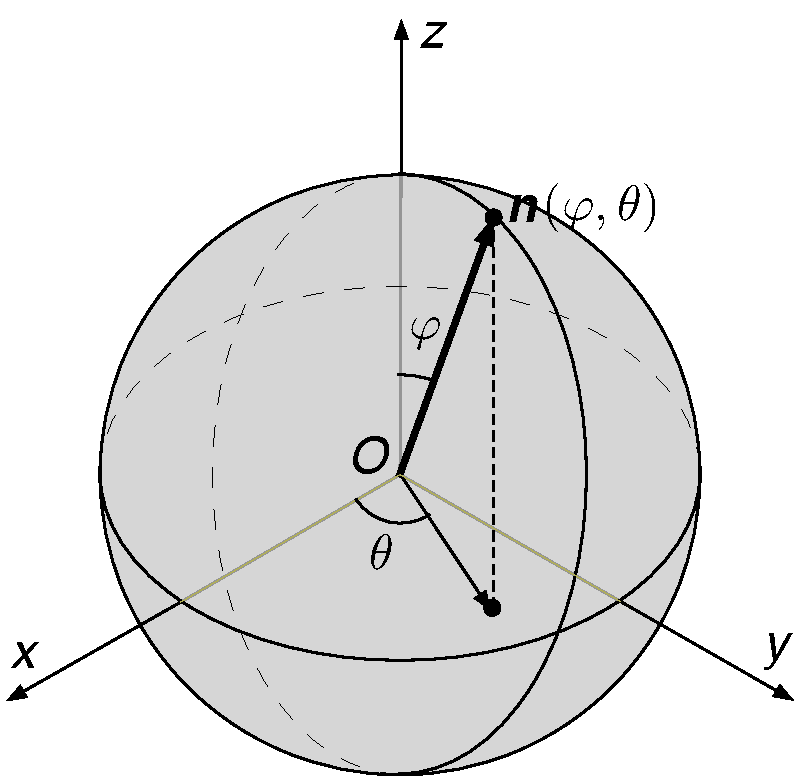
\includegraphics[width=75mm]{figs/spherical.pdf}
      \label{fig:spherical}
    }
    \subfigure[Stereographic]{
      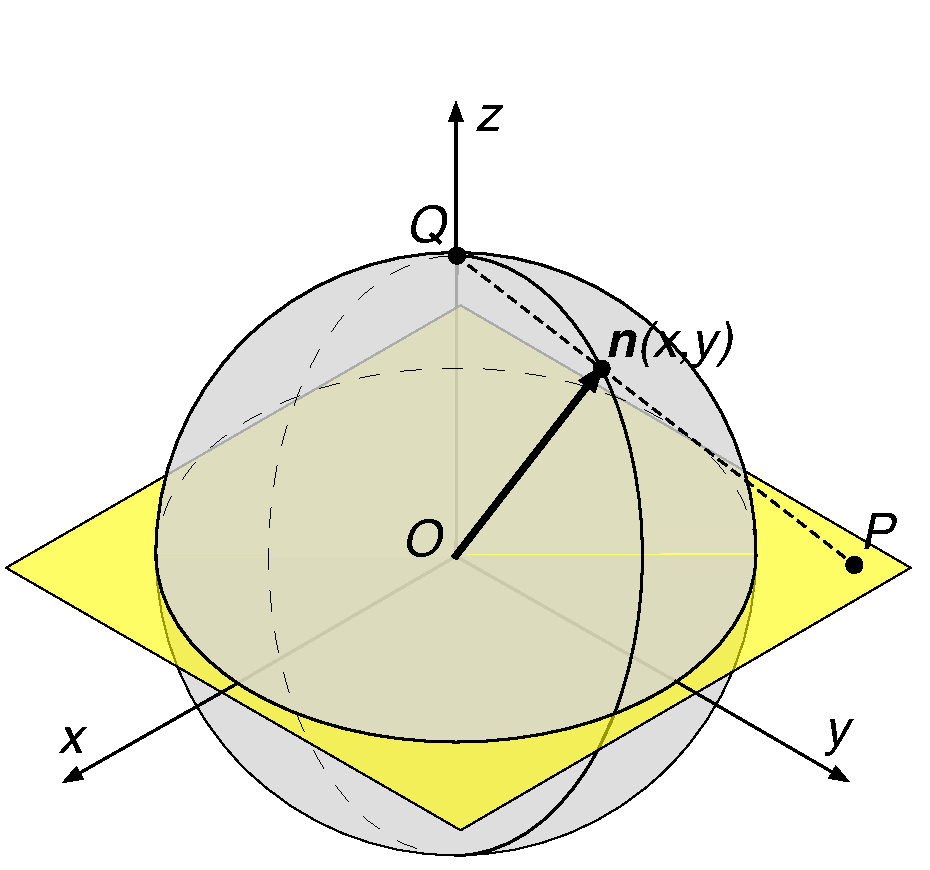
\includegraphics[width=75mm]{figs/stereographic.pdf}
      \label{fig:stereographic}
    }
    \subfigure[Projective]{
      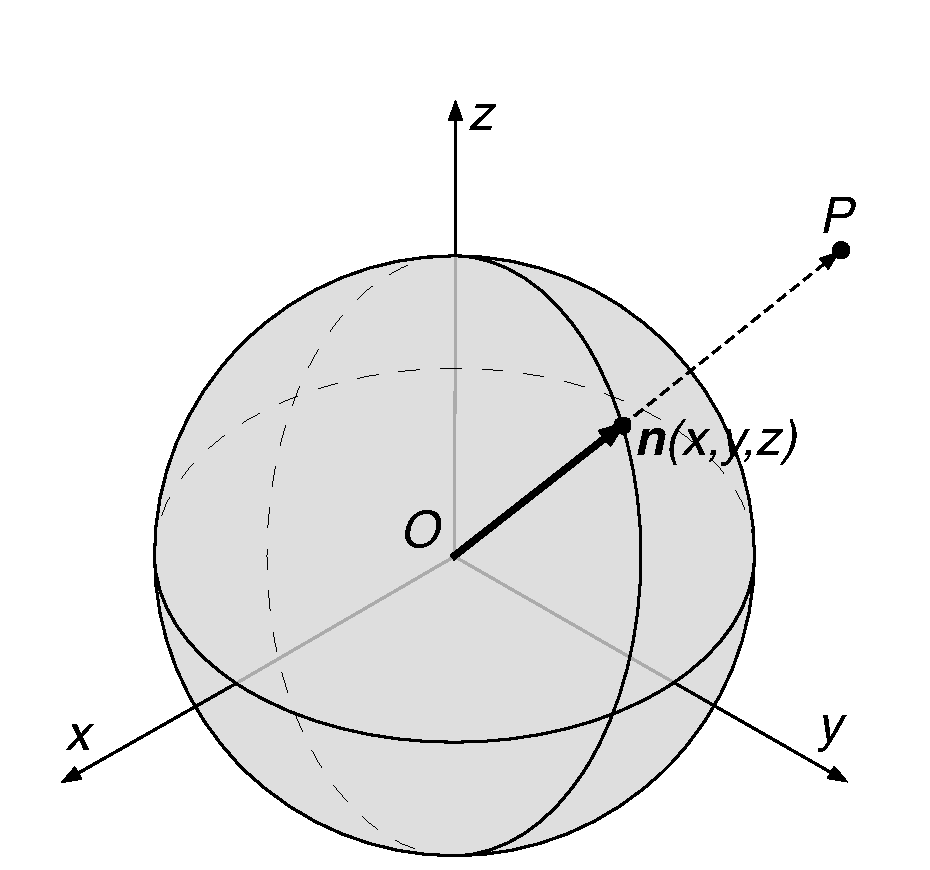
\includegraphics[width=75mm]{figs/projective.pdf}
      \label{fig:projective}
    }
    \subfigure[Tangent]{
      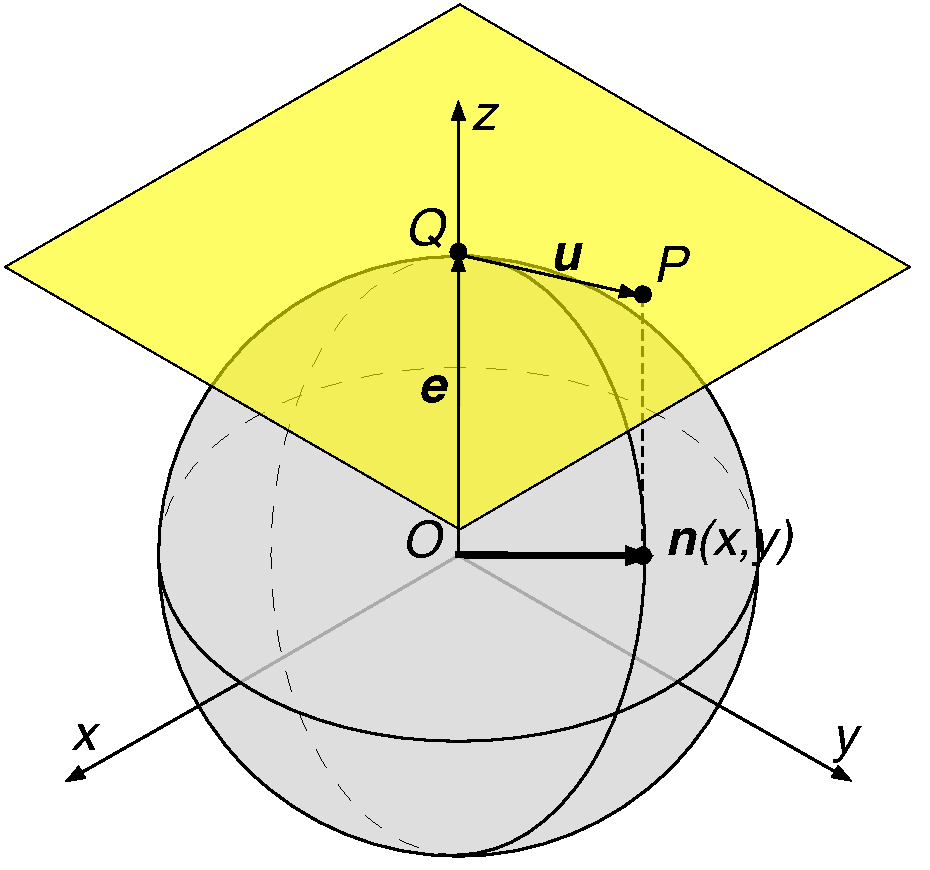
\includegraphics[width=75mm]{figs/tangent.pdf}
      \label{fig:tangent}
    }
    \subfigure[Cartesian]{
      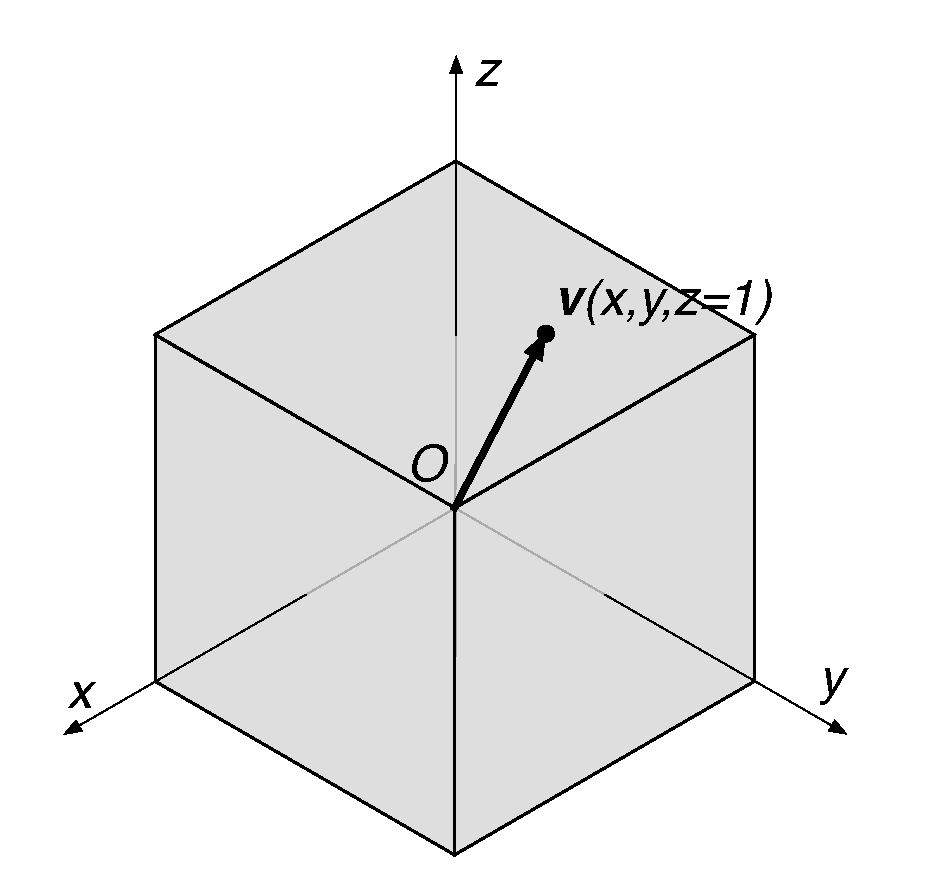
\includegraphics[width=75mm]{figs/cartesian.pdf}
      \label{fig:Cartesian}
    }
    \caption{The five parametrizations used for the detection of loss
      of ellipticity.}
    \label{fig:parametrizations}
  \end{center}
\end{figure}

\section{Bifurcation Detection}
\label{sec:detection}

Within an incremental update setting, the numerical detection of the
bifurcation condition for each time increment using any of the
parametrizations just described consists of the following two steps:

\begin{itemize}

\item An initial sampling is performed over the parametric space for
  $~q$ for the normal vector $~n \in S^2$ or $~v \in \{ ~u \in {"R}^3
  | \, ||~u||_\infty = 1\}$ associated with the parametrization. This
  leads to a rough estimate of the minimum of the determinant function
  \eqref{eq:minimization-determinant} and the associated bifurcation
  directions.

\item The coarse estimate can be used to initiate an iterative
  procedure to find a more accurate estimate of the onset of
  bifurcation and its associated directions by solving the
  optimization problem \eqref{eq:minimization-derivative}.

\end{itemize}

In an actual finite element simulation, the above two-step procedure
may not yield estimates of the bifurcation condition that are accurate
enough within a time increment, in particular if the size of the
increment is relatively large. One way to improve the solution is to
introduce adaptive time increments for the detection of the
bifurcation condition.  Define
\begin{equation} \label{eq:general-minimization-problem}
  \mu_{n+1,k} := \min_{~q} f_{n+1,k}(~q) = \min_{~q} \det ~B_{n+1,k}(~q)
\end{equation}
where the tensor $~B_{n+1,k}(~q)$ may be either the one from
\eref{eq:acoustic-tensor} or the one from
\eref{eq:Cartesian-acoustic-tensor}, depending on the parametrization
in use, and the index ${n+1,k}$ indicates that the evaluation occurs
at time $t_{n+1,k} \in [t_n, t_{n+1}]$.

Consider the original time increment from $t_n$ to $t_{n+1}$, where
$\mu_n > 0$ and $\mu_{n+1} < 0$. This means that between time $t_n$
and $t_{n+1}$, the strong ellipticity condition is violated and hence
the material exhibits bifurcation. Assume also that $\mu_n / \mu_0 >
\epsilon$, where $\mu_0$ is the value of the determinant function
evaluated at time $t_0$ and $\epsilon$ is a target tolerance. We wish
to find a better estimate for the determinant function $\mu_{n+1,k}$,
and hence the bifurcation time $t_{n+1,k}$, such that $\mu_{n+1,k} /
\mu_0 \le \epsilon$. This is achieved by an adaptive time increment
procedure by means of bisection, as shown in
Algorithm~\ref{alg:adaptive-step}. This algorithm repeatedly cuts the
time increment in half until the convergence criterion $\mu_{n+1,k} /
\mu_0 \le \epsilon$ is met.

\begin{algorithm}[!htbp]
  \caption{$\text{AdaptiveStep}(\mu_0, \mu_{n+1}, t_{n+1}, \epsilon)$}
  \begin{algorithmic}
    \REQUIRE $\mu_{n+1} < 0$
    \ENSURE $\mu_{n+1,k} \in [0, \epsilon \mu_0]$
    \STATE initialize
    $k \leftarrow 1,
    \quad
    \alpha \leftarrow \frac{1}{2},
    \quad
    \triangle t \leftarrow t_{n+1} - t_n,
    \quad
    \mu_{n+1,k} \leftarrow \mu_{n+1}$
    \WHILE{ $\mu_{n+1,k} < 0$ {  or  } $ \mu_{n+1,k} / \mu_0
      > \epsilon$ }
    \STATE $t_{n+1,k} \leftarrow t_n + \alpha \triangle t$
    \STATE compute $~F(t_{n+1,k})$ using the global solution scheme
    \STATE compute $\triangle ~Z(t_{n+1,k})$
    by solving \eref{eq:Biots-equation-discrete}
    \STATE compute $\bbA(t_{n+1,k})$
    using \eref{eq:incremental-stress-moduli}
    \STATE compute $\mu_{n+1,k}$
    by solving \eref{eq:general-minimization-problem}
    \IF{$\mu_{n+1,k} > 0$}
    \STATE $\alpha \leftarrow \alpha + 2^{-k-1}$
    \ELSE
    \STATE $\alpha \leftarrow \alpha - 2^{-k-1}$
    \ENDIF
    \STATE $k \leftarrow k+1$
    \ENDWHILE
  \end{algorithmic}
  \label{alg:adaptive-step}
\end{algorithm}

The adaptive time increment procedure allows the accurate (up to the
tolerance $\epsilon$) detection of the bifurcation time during a
loading process. The procedure described in this section to detect
material bifurcation can be applied to a very general class of
materials and its numerical performance is demonstrated in the
following section.

\section{Numerical Examples}
\label{sec:numerical-examples}

The performance and applicability of the proposed Cartesian and the
other four parametrizations are examined by using them for the
bifurcation analysis of two material models under different loading
conditions. The analysis is performed at the material point level. Of
particular interest are the robustness and computational efficiency of
the different parametrizations.

\subsection{Small Deformation Isotropic Elastic Damage Model}
\label{subsec:isotropic}

We start the bifurcation analysis on a simple small deformation
isotropic damage model. The model formulation is briefly presented
first. The material model is then subjected to simple shear to
determine the performance of the different parametrizations on the
detection of material bifurcation.

\subsubsection{Model Formulation}

The stress and constitutive tangent of the small deformation isotropic
damage model are derived from the strain-energy function that has the
form
\begin{equation}\label{eq:iso-psi}
  A(\bepsilon ^e, \xi)
  :=
  \frac{1}{2} (1 - \xi)
  \bepsilon ^e : \mathbb{C}^e : \bepsilon ^e
\end{equation}
where $\bepsilon^e$ is the infinitesimal elastic strain tensor,
$\bbC^e$ is the fourth-order elastic moduli tensor, and $\xi$ is a
damage parameter introduced to trigger material bifurcation. For
isotropic linear elasticity, the elastic moduli tensor $\bbC^e$ is
given as
\begin{equation}
  \bbC^e := \lambda ~I \otimes ~I + 2\mu \bbI
\end{equation}
where $\lambda$ and $\mu$ are the Lam\'{e} constants, $~I$ is the
second-order identity tensor and $(\bbI)_{ijkl} =
\frac{1}{2}(\delta_{ik}\delta_{jl} + \delta_{il}\delta_{jk})$ is the
fourth-order symmetric identity tensor with $\delta_{ik}$ being the
Kronecker delta.

We adopt the following evolution law for the scalar damage parameter $
\xi$ \cite{Holzapfel:2000}
\begin{equation}\label{eq:iso-xi}
  \xi(\alpha) := \xi_{\infty} [ 1- {\rm exp}(-\alpha / \tau)]
\end{equation}
where $\xi_{\infty}$ describes the dimensionless maximum damage and
$\tau$ is referred to as the damage saturation parameter. The
parameter $\alpha$ is the maximum thermodynamic force
\cite{Holzapfel:2000} with the same dimensions as the effective strain
energy. Within the closed time interval $[0,t]$, $\alpha$ is given as
\begin{equation}\label{eq:alpha}
  \alpha(t) := \max_{s\in [0,t]}A_0(s)
\end{equation}
where $A_0(s)$ is the undamaged strain energy at time $s$.

Given the strain-energy function \eref{eq:iso-psi} and the damage
evolution \eref{eq:iso-xi}, the fourth-order tangent moduli tensor can
be obtained by differentiating the strain-energy function with respect
to the strain measure $\bepsilon_e$ twice, which results in
\begin{equation}
  \bbC := (1-\xi)\bbC^e
    - \beta \frac{\partial\xi}{\partial\alpha}
    (\bsigma_0\otimes\bsigma_0)
\end{equation}
where $\bsigma_0$ is the effective (undamaged) Cauchy stress and
$\beta = 1 \iff \dot{\alpha} > 0$, $\beta=0$ otherwise. In a small
deformation setting, this tangent can be used to compute the acoustic
tensor \eref{eq:acoustic-tensor}, which can then be tested for
material bifurcation.

\subsubsection{Simple Shear Test}

In this section, a simple shear test illustrated in Figure~\ref{fig:simple_shear} is simulated with the following
material properties: $\lambda = 80$, $\mu = 80$, $\xi_{\infty} = 1.0$
and $\tau = 1.0$. The resulting shear stress and shear strain are
plotted in \fref{fig:iso-stress_strain}(a). The softening response is
due to the evolution of the introduced damage parameter $\xi$.
\begin{figure}[!htbp]
 \centering
      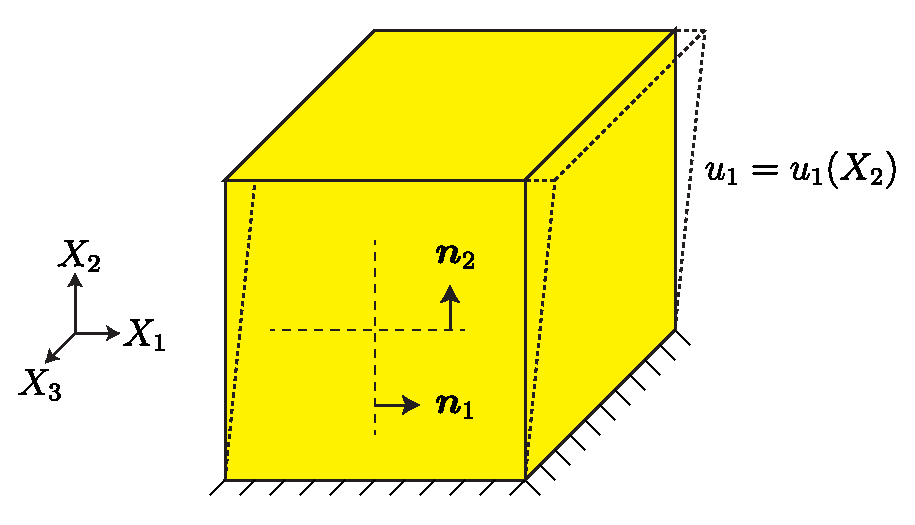
\includegraphics[width=0.5\textwidth]{figs/simple_shear_schematic.pdf}
     \caption{Schematic of the the applied loading for simple shear under for infinitesimal deformations. The solution bifurcates on planes with normals $\bn_{1}$ and $\bn_{2}$.}
      \label{fig:simple_shear}
\end{figure}
For the numerical detection of material bifurcation, the two-step
procedure described in \sref{sec:detection} is adopted, \ie, (1) an
initial sampling performed over the parametric space, and (2) a Newton
iterative procedure to obtain a better estimate of the onset of
bifurcation and its associated directions.
\fref{fig:iso-stress_strain}(b) shows the degradation of the
determinant $\det~A$ for all five parametrizations up to the point
when material bifurcation is detected. When det$~A = 0$, the material
model bifurcates. In this example, all five parametrizations detect
bifurcation at the same time, \ie, when the shear strain
$\epsilon_{12}=0.0559$ as marked in \fref{fig:iso-stress_strain}
(a). With the adaptive time step algorithm the precise time of
bifurcation, up to the specified tolerance, can be detected.

\begin{figure}[!htbp]
  \centering \subfigure[]{
    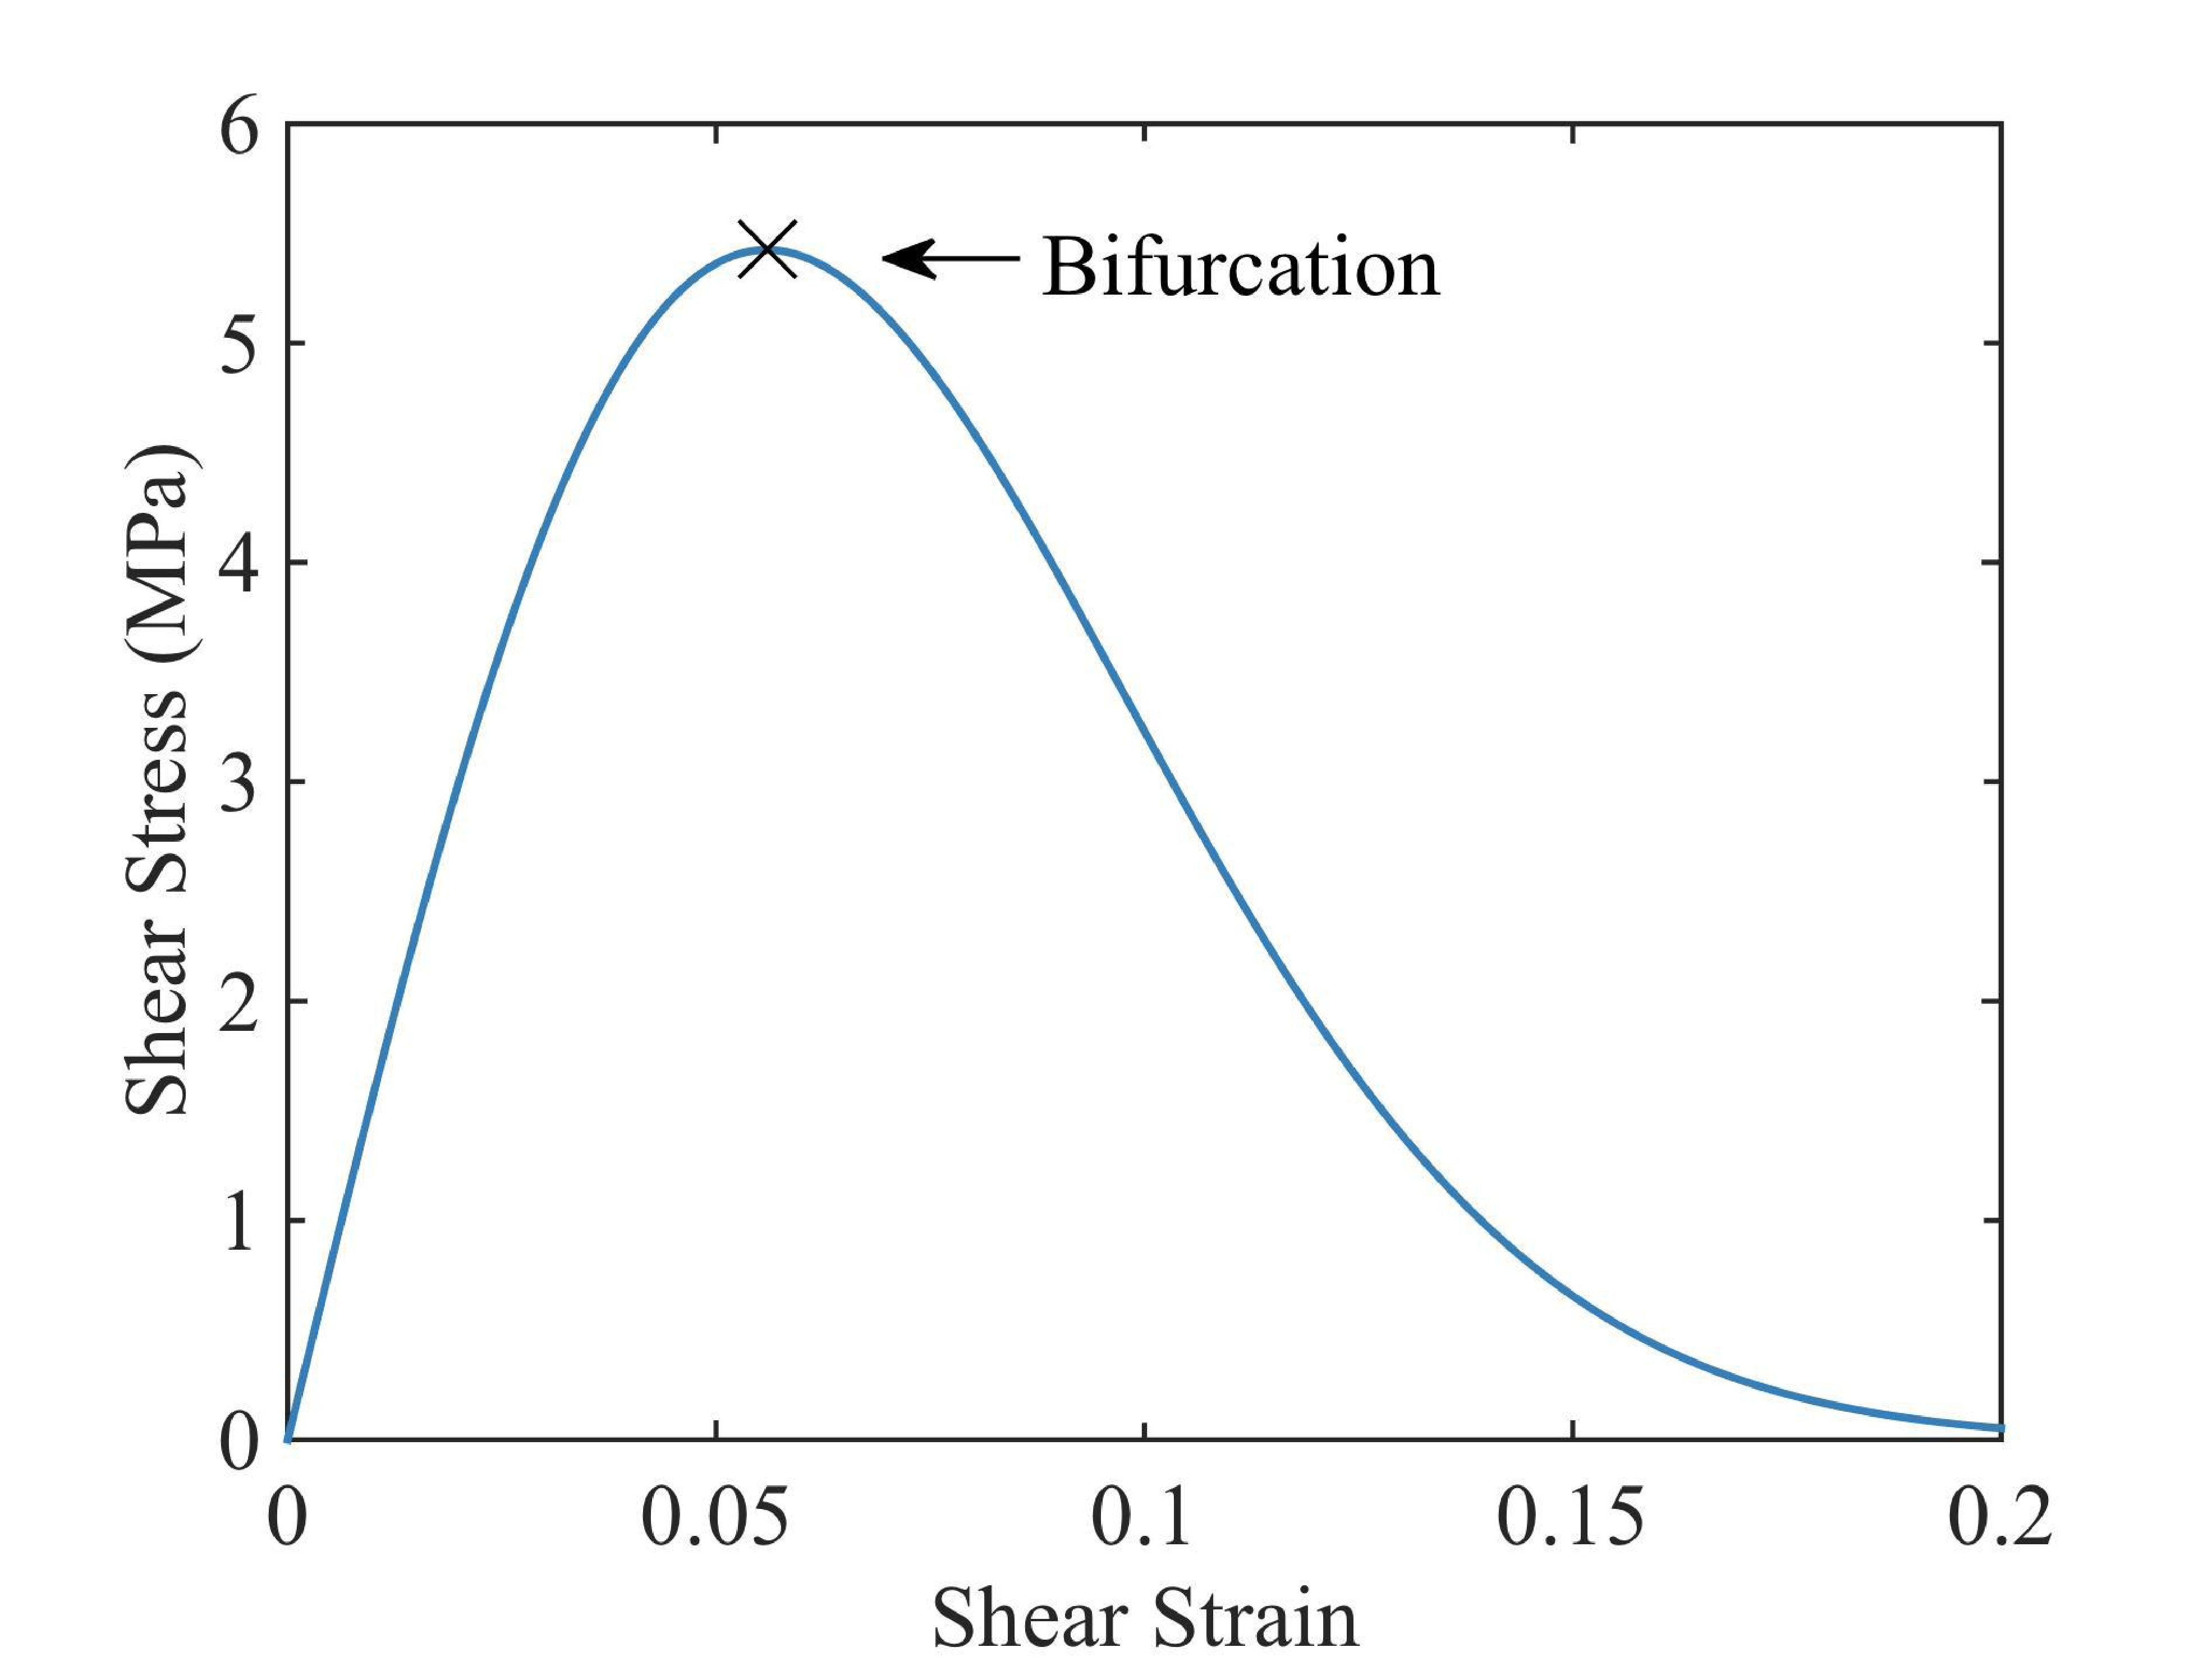
\includegraphics[width=0.60\textwidth]
                    {figs/iso_shear_stress_strain.pdf}
  } \subfigure[]{
    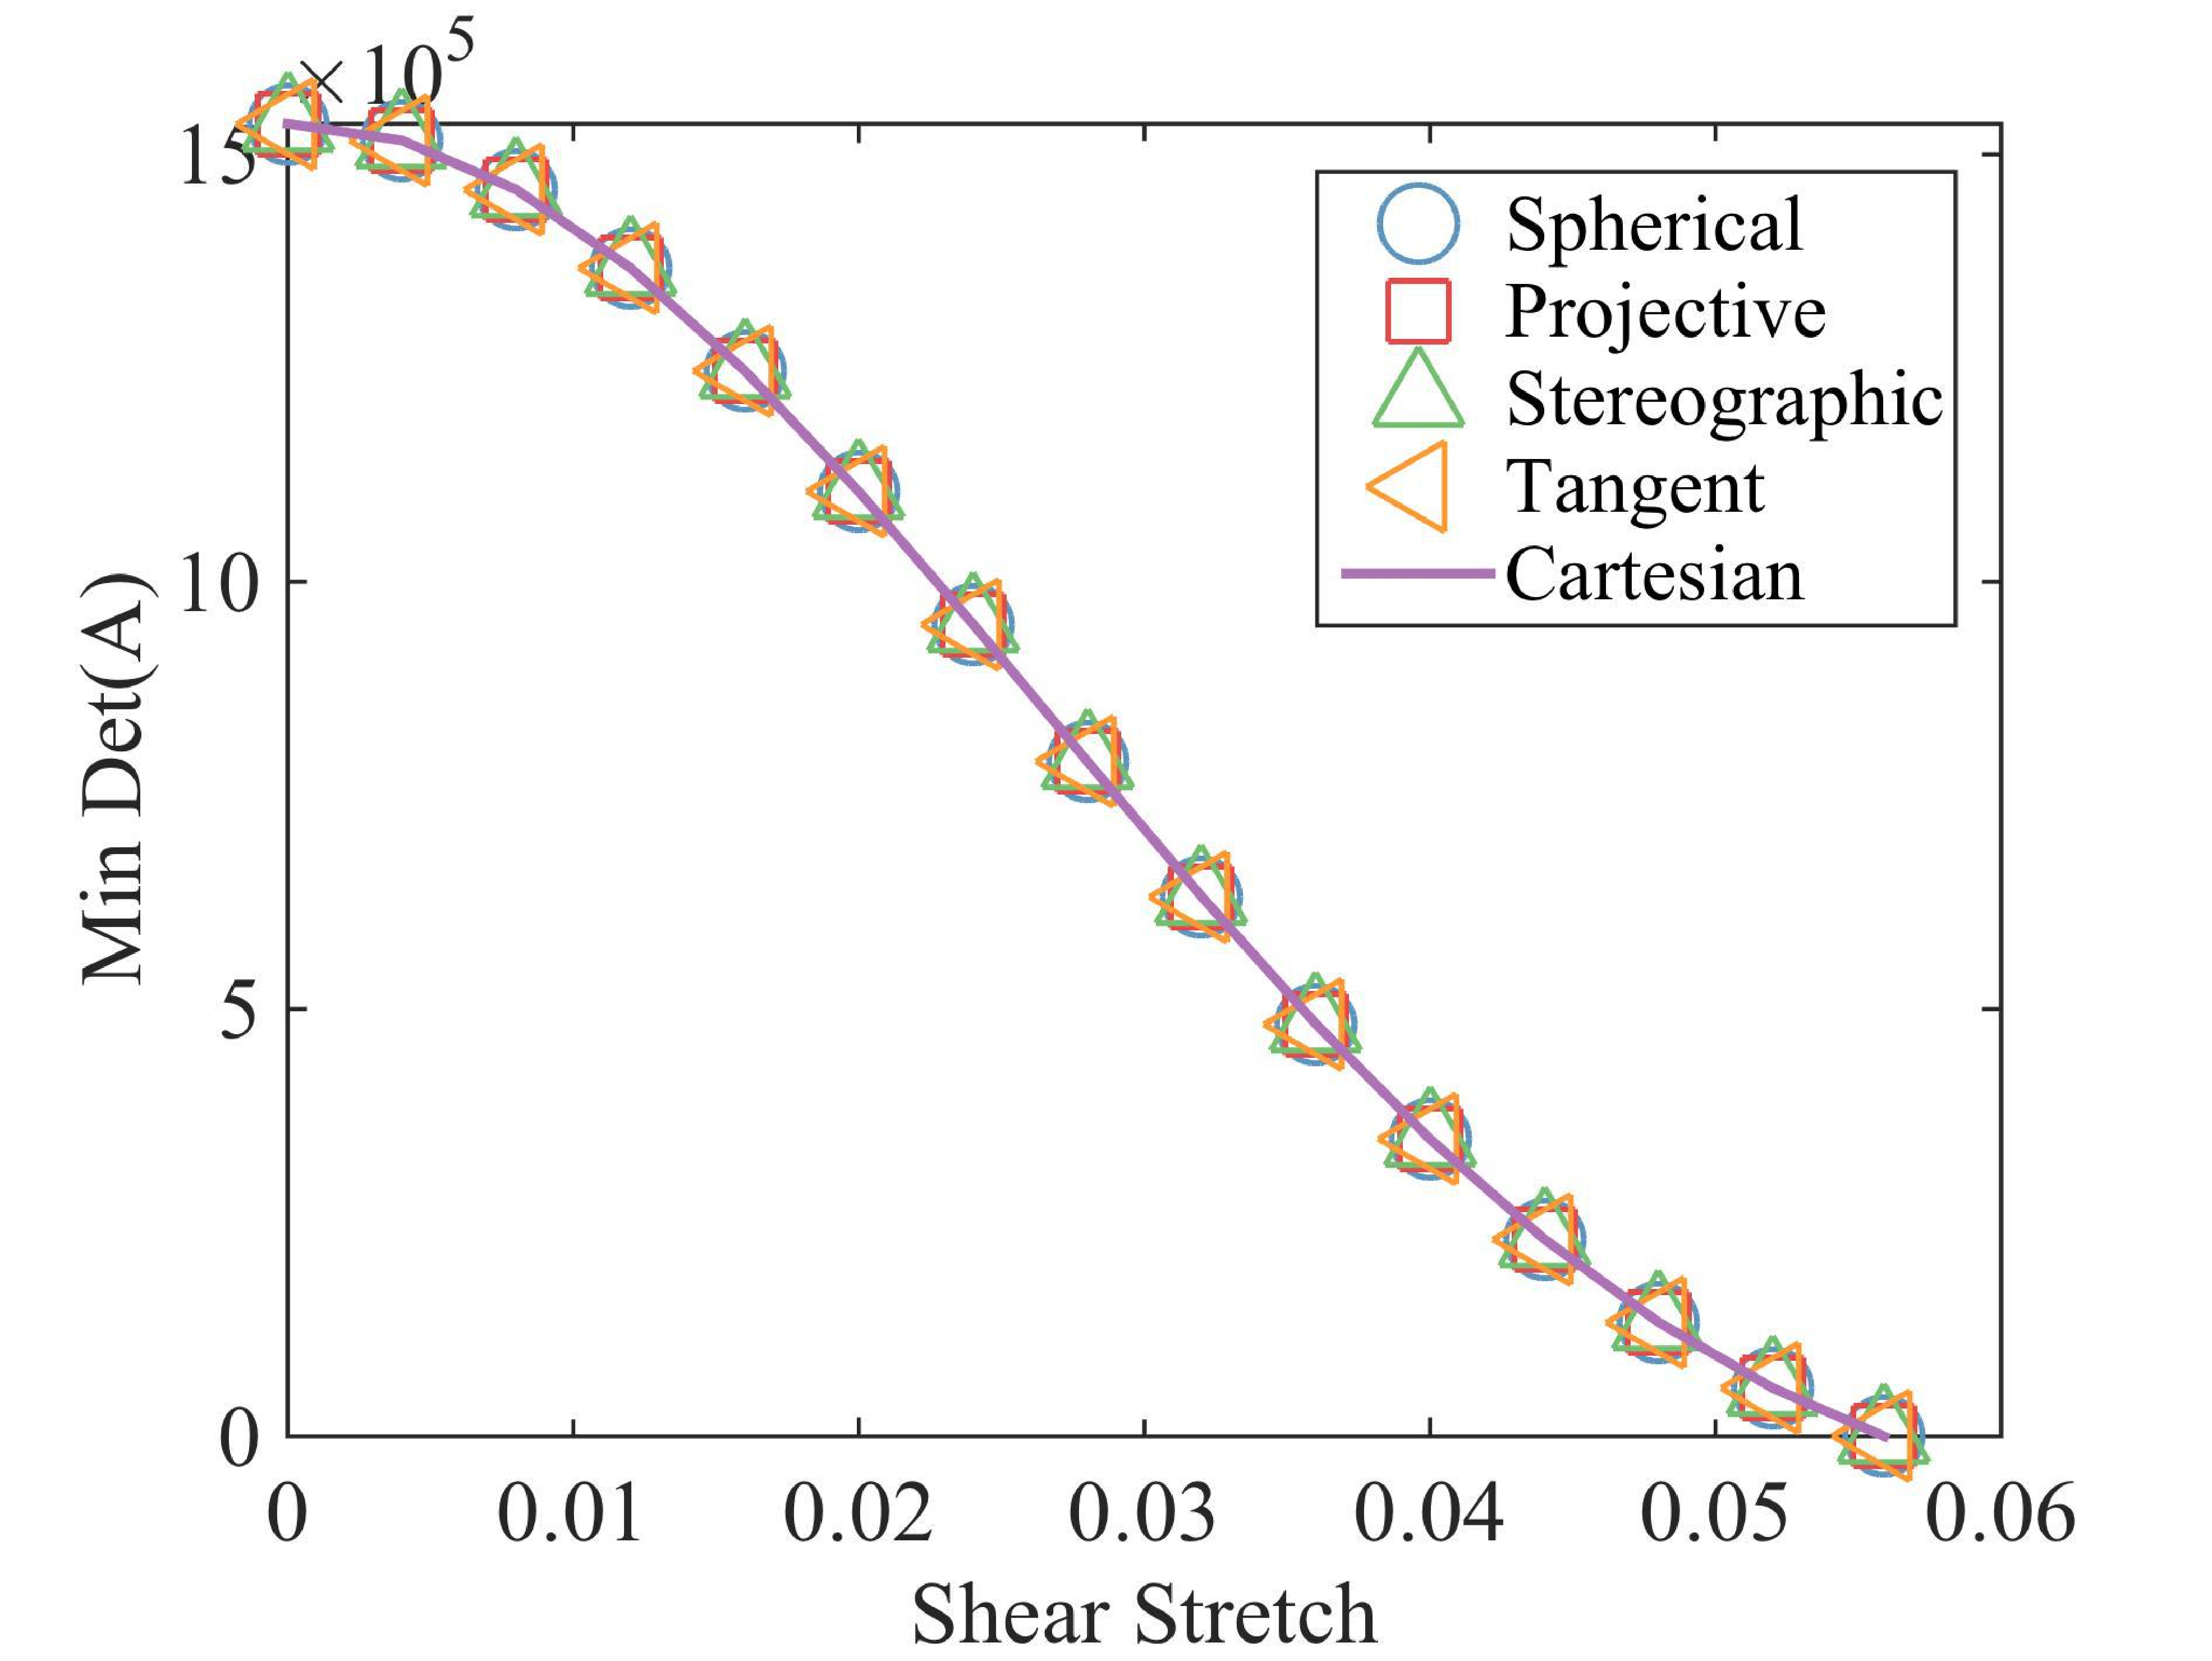
\includegraphics[width=0.60\textwidth]
                    {figs/iso_shear_mindetA_strain.pdf}
  }
  \caption{Simple shear test on small deformation isotropic damage
    model: (a) stress strain behavior, with the X indicating
    bifurcation, and (b) degradation of $\det~A$ for different
    parametrizations upto the point material bifurcates
    ($\epsilon_{12}=0.0559$).}
  \label{fig:iso-stress_strain}
\end{figure}

While all five parametrizations detect bifurcation at the same time,
\fref{fig:iso-stress_strain}(b) provides little information on their
computational efficiency and robustness, which are the focus of this
work. The computational cost of bifurcation detection mainly consists
of two parts: (1) the computation time of the initial sampling over
the parametric space, and (2) the computation time of the Newton
iterative scheme.

The computation time of the initial sampling depends on the number of
sampling points, or equivalently, the density of the initial sampling
grid. The denser the initial sampling grid, the more expensive it is
computationally to perform a complete pass of all the points in the
grid. The computation time for the Newton iterative scheme, on the
other hand, depends mainly on the complexity of the objective
function, \ie, $\det~A$, as well as the quality of the initial guess.

To compare computational costs of different parametrizations, we
record the time spent on the bifurcation detection at a particular
loading increment, \eg, at the increment leading to bifurcation. We
also vary the density of the initial sampling grid to determine its
effect on different parametrizations. The density of the initial sampling grid is represented by the sampling interval and the number of sampling points, as shown in \fref{fig:interval_scheme}.

\begin{figure}[!htbp]
  \centering 
    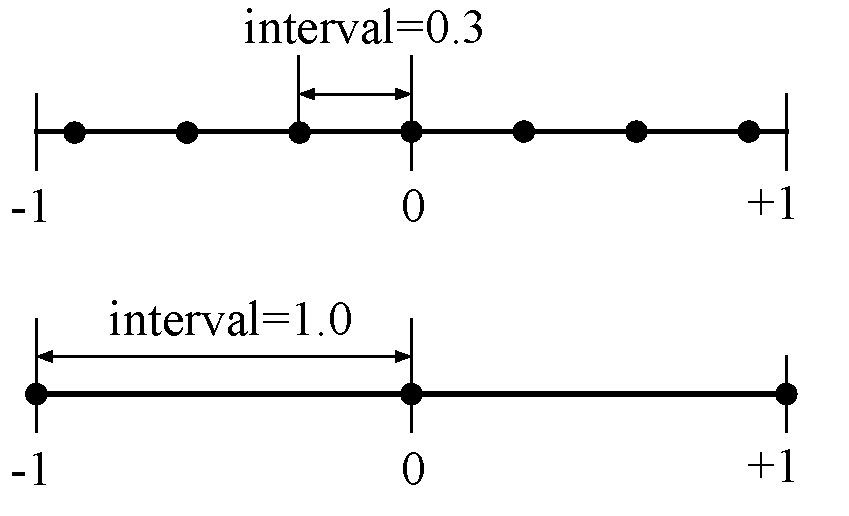
\includegraphics[width=0.4\textwidth]
                    {figs/interval_scheme.pdf}
  \caption{Schematic drawing shows the interval along one dimension 
  of the normalized parameter space $[-1, 1]$ for the cases 
  of interval = 0.3 (top) and interval = 1.0 (bottom). Black solid 
  circles indicate the locations of grid points}
  \label{fig:interval_scheme}
\end{figure}

A robust parametrization should be insensitive to the initial 
sampling grid.The computation time results are summarized in Table~
\ref{tab:iso-shear-runtime}. The table only shows the number of 
sampling points, $N$, along one dimension of the parametric space. 
Assuming the same number of intervals for each parameter, the total 
number of sampling points is $N^{D}$ where $D$ is the total dimension 
of the parametric space.

As expected, it can be seen from Table~\ref{tab:iso-shear-runtime}
that as the number of sampling points $N$ per dimension decreases, so
does the computational cost. The spherical and the Cartesian
parametrizations are the most efficient. The stereographic, projective
and tangent parametrizations are more computationally expensive. In
the extreme case with $N=1$ \ie only one initial sampling point, the
stereographic, projective and tangent parametrizations fail to
correctly detect bifurcation, shown as a dash in the table.

\begin{table}[!htbp]
  \begin{center}
    \begin{tabular}{c c | r r r r r}
      \toprule
      \multicolumn{2}{c}{Sampling} & \multicolumn{5}{c}{Run Time ($\mu$s)} \\
      Interval & Points & Spherical & Stereographic & Projective &
      Tangent & Cartesian \\
      \midrule
      0.05 & 41 & 318 & 155 & 5636 & 226 & 347  \\
      0.1 & 21 & 124 & 89  & 884 & 107 & 115  \\
      0.2 & 11 & 70 & 60  & 183 & 64  & 81  \\
      0.3 & 7 & 63 & 184 & 178 & 157 & 39  \\
      0.4 & 5 & 73 & 181 & 197 & 145 & 27  \\
      0.5 & 5 & 51 & 37  & 88  & 53  & 27  \\
      0.6 & 3 & 62 & 174 & 200 & 215 & 23  \\
      0.7 & 3 & 61 & 180 & 188 & 188 & 23  \\
      0.8 & 3 & 50 & 170 & 188 & 144 & 24  \\
      0.9 & 3 & 51 & 177 & 156 & 159 & 23  \\
      1.0 & 3 & 47 & 37  & 79  & 51  & 23  \\
      1.5 & 1 & 51 & -- & --  & -- & 21  \\
      \bottomrule
    \end{tabular}
    \caption{Computational cost of different parametrizations in
      simple shear test at loading increment leading to bifurcation.
      The dash ``--'' indicates that the parametrization fails to
      detect bifurcation in this loading increment.}
    \label{tab:iso-shear-runtime}
  \end{center}
\end{table}

As mentioned before, the choice of parametrization directly affects
the complexity of the objective function $\det~A$ in
\eref{eq:minimization-derivative}. This in turn affects the
computational efficiency and robustness of the different
parametrizations for the detection of material bifurcation, as shown
in Table~\ref{tab:iso-shear-runtime}. To illustrate this point, the
landscapes of the objective function $\det~A$ at bifurcation, \ie, at
$\bepsilon_{12}=0.0559$ are shown in \fref{fig:iso-shear-detA}. The
corresponding plane views of the determinant landscapes are shown in
\fref{fig:iso-shear-detAXplane}, where the white stars indicate global
minima. The projective parametrization requires three parameters and
therefore it is not shown.

\begin{figure}[!htbp]
   \centering \subfigure[Spherical]{
   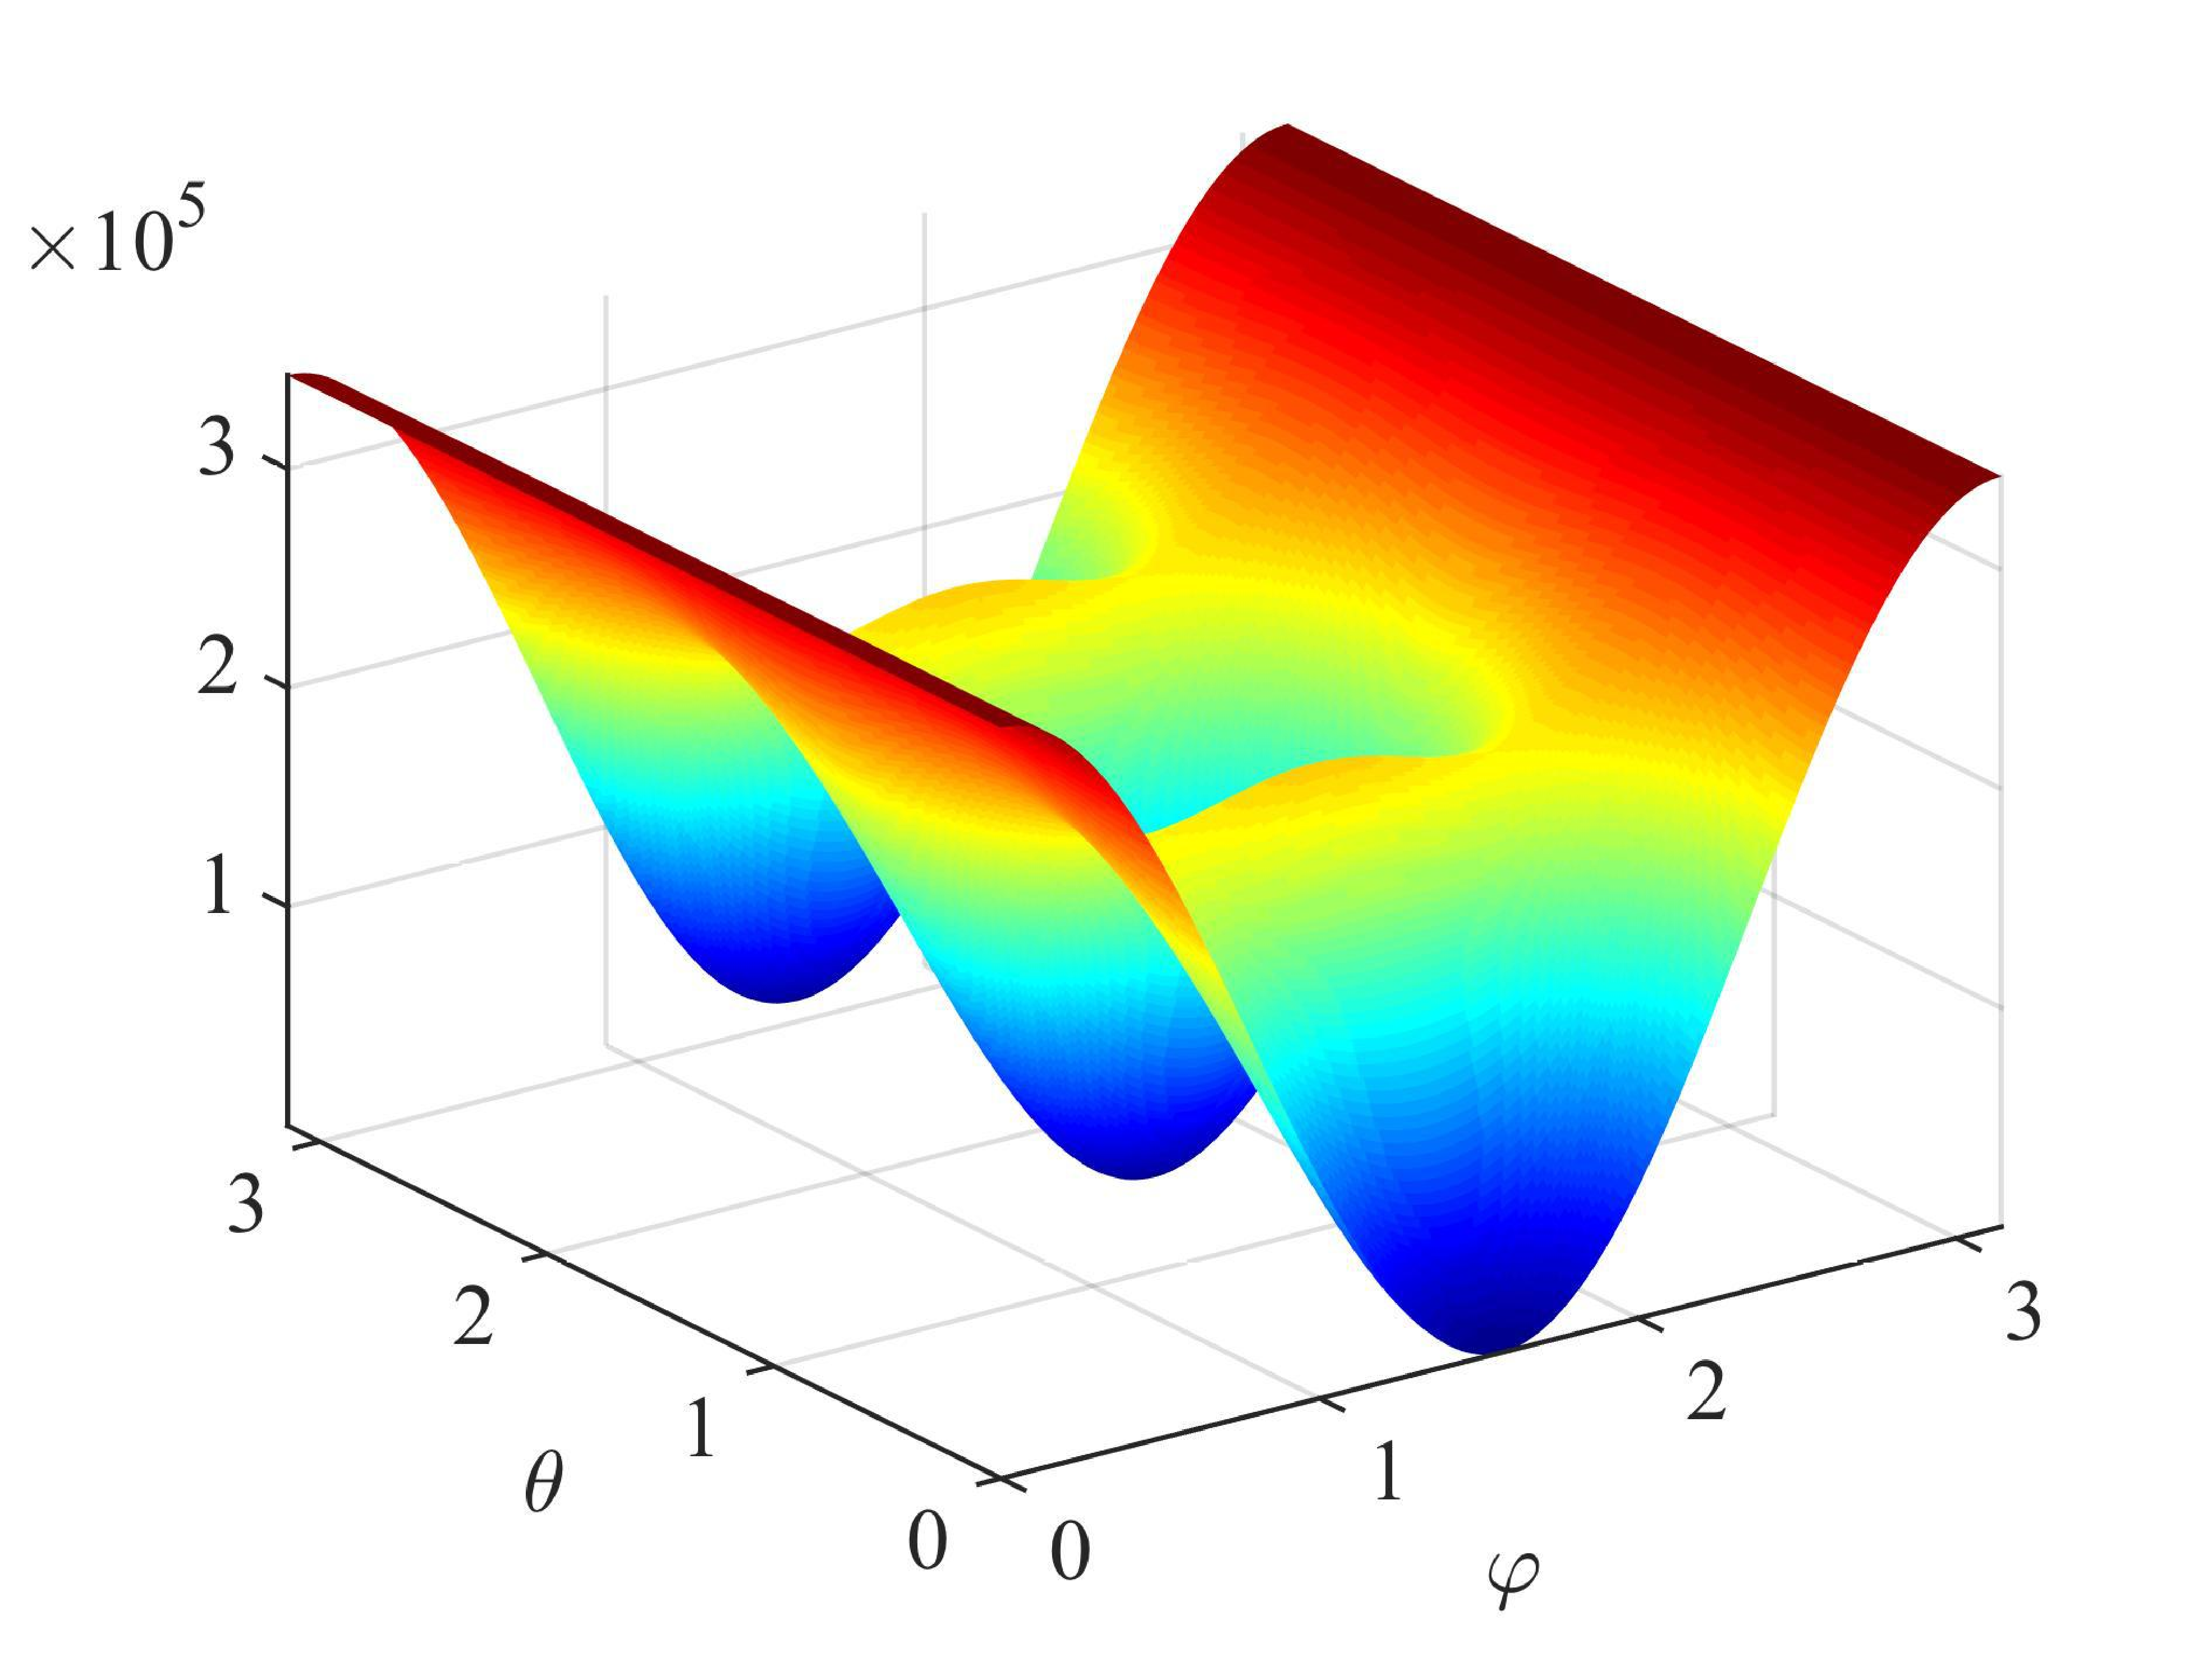
\includegraphics[width=0.45\textwidth]
   {figs/iso_shear_spherical_detA.pdf}
 } \subfigure[Cartesian]{
   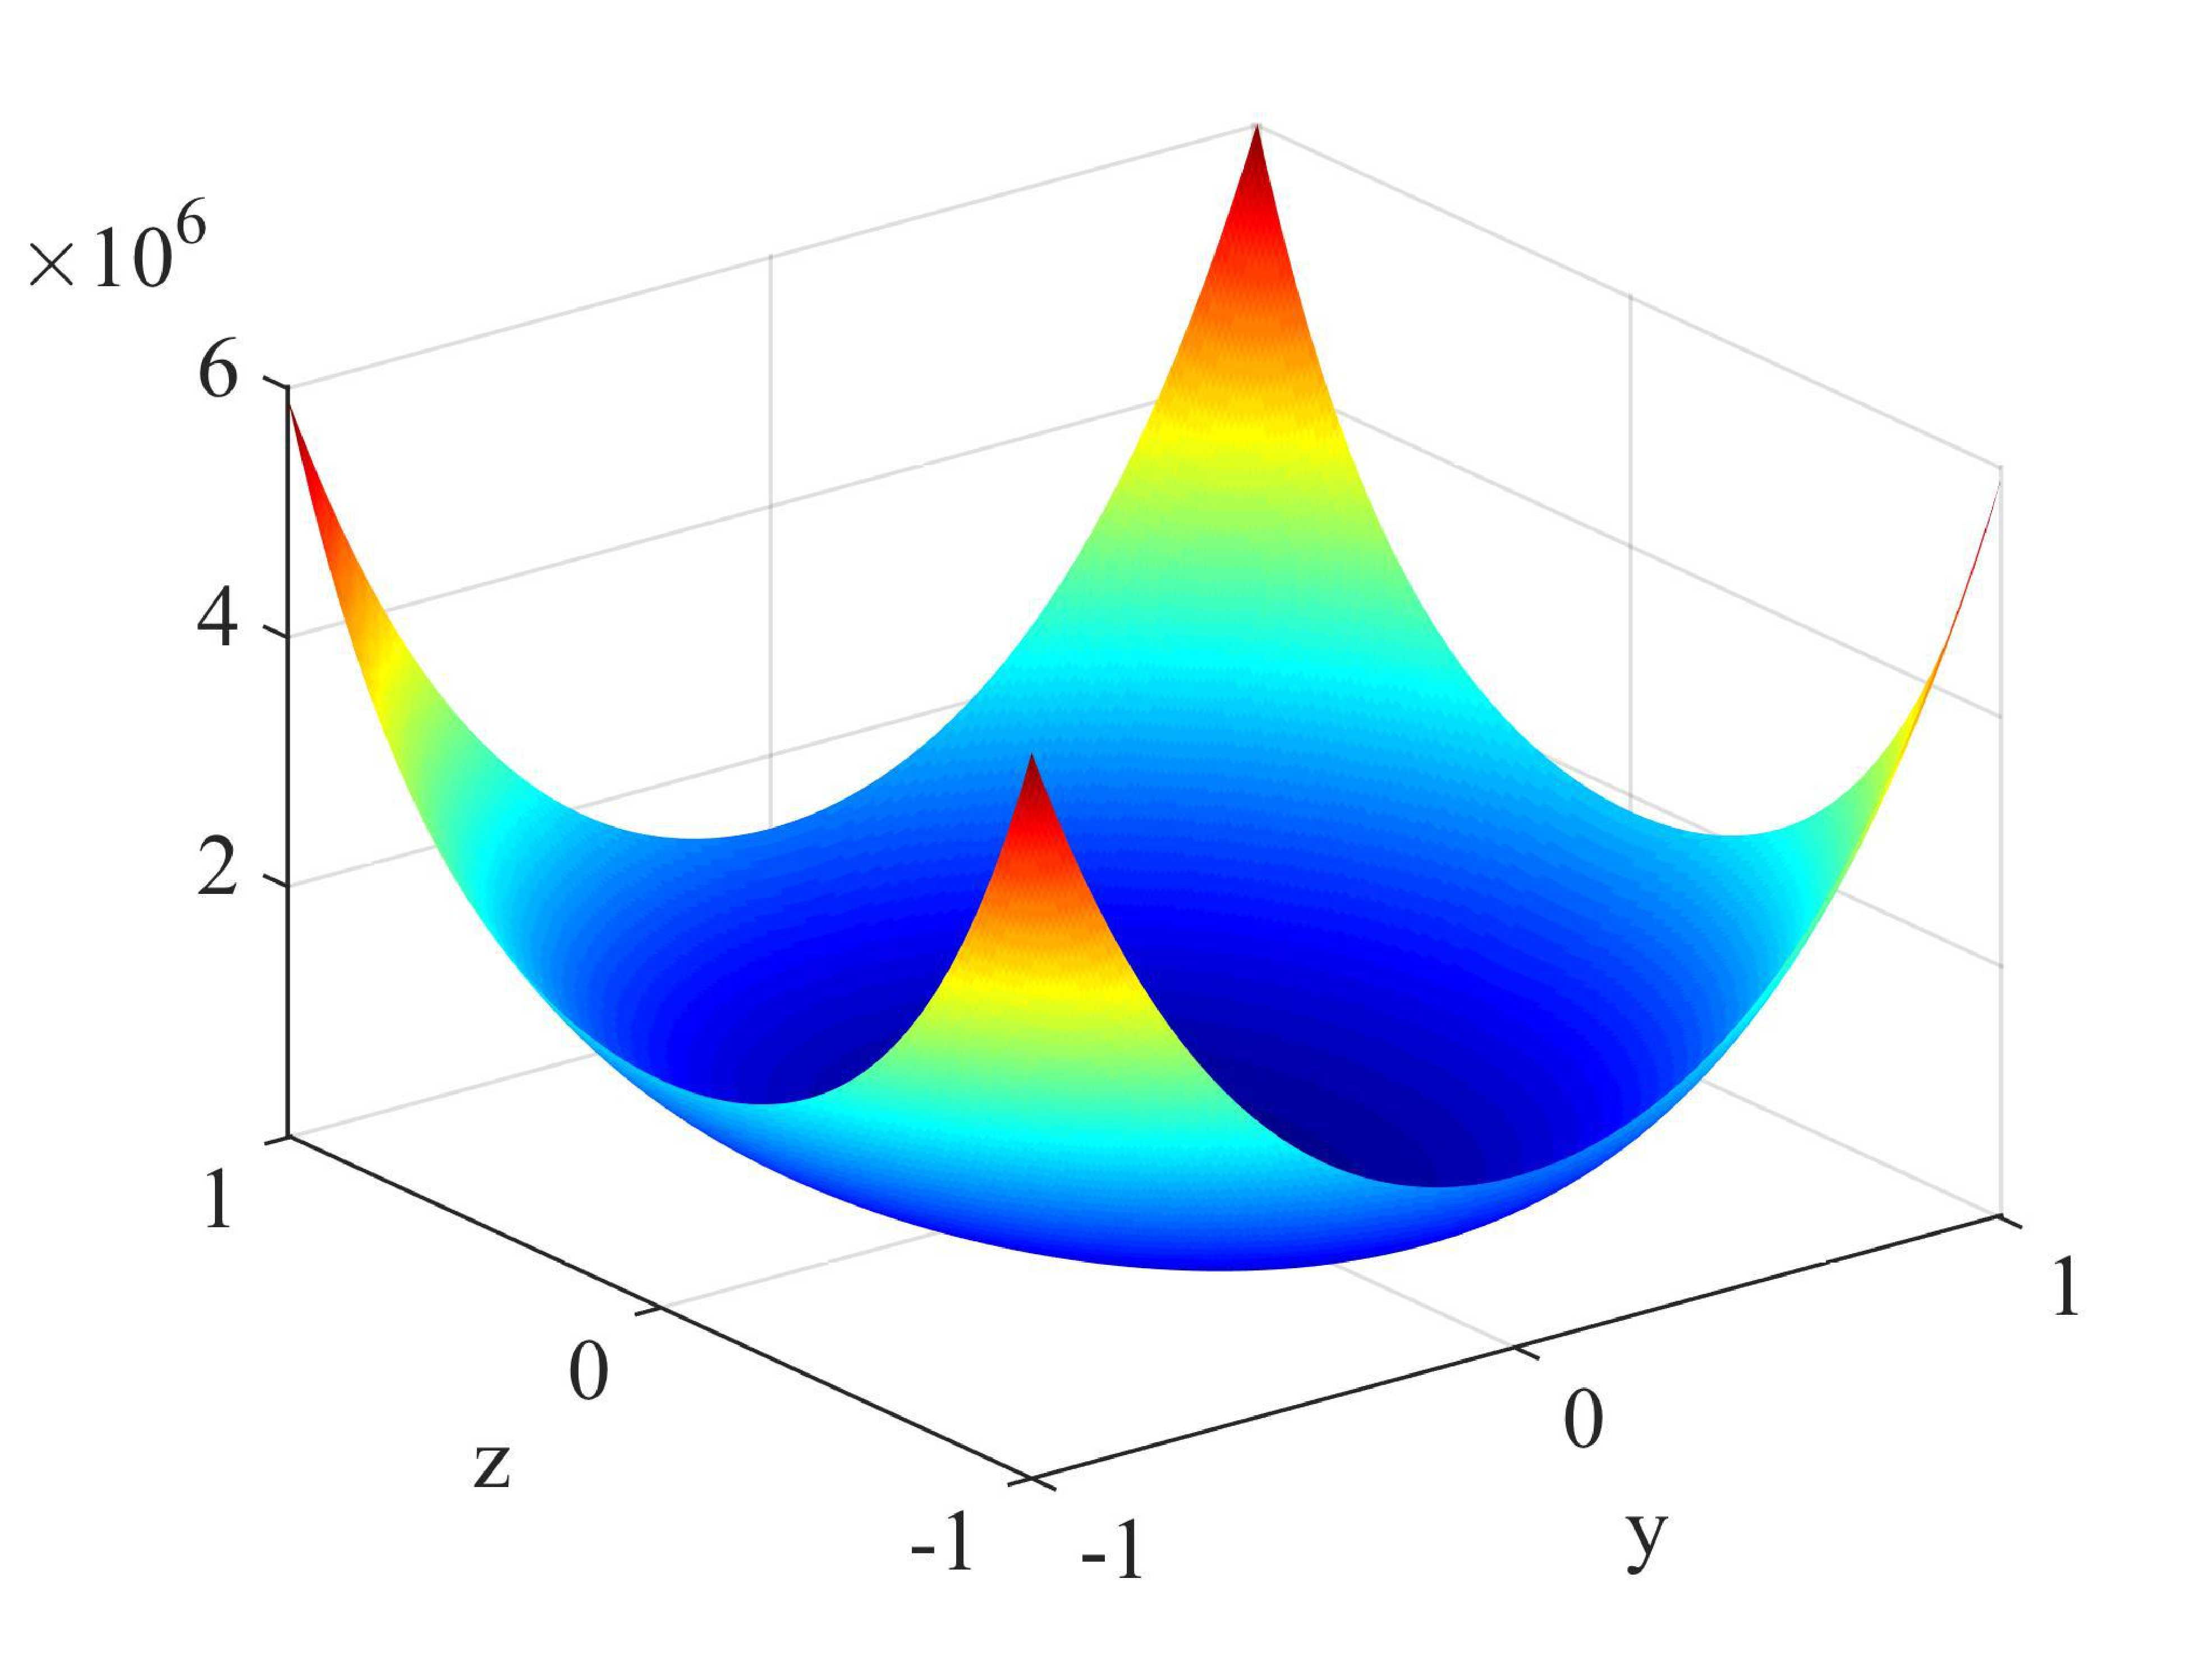
\includegraphics[width=0.45\textwidth]
   {figs/iso_shear_cartesian_detA.pdf}
 } \subfigure[Stereographic]{
   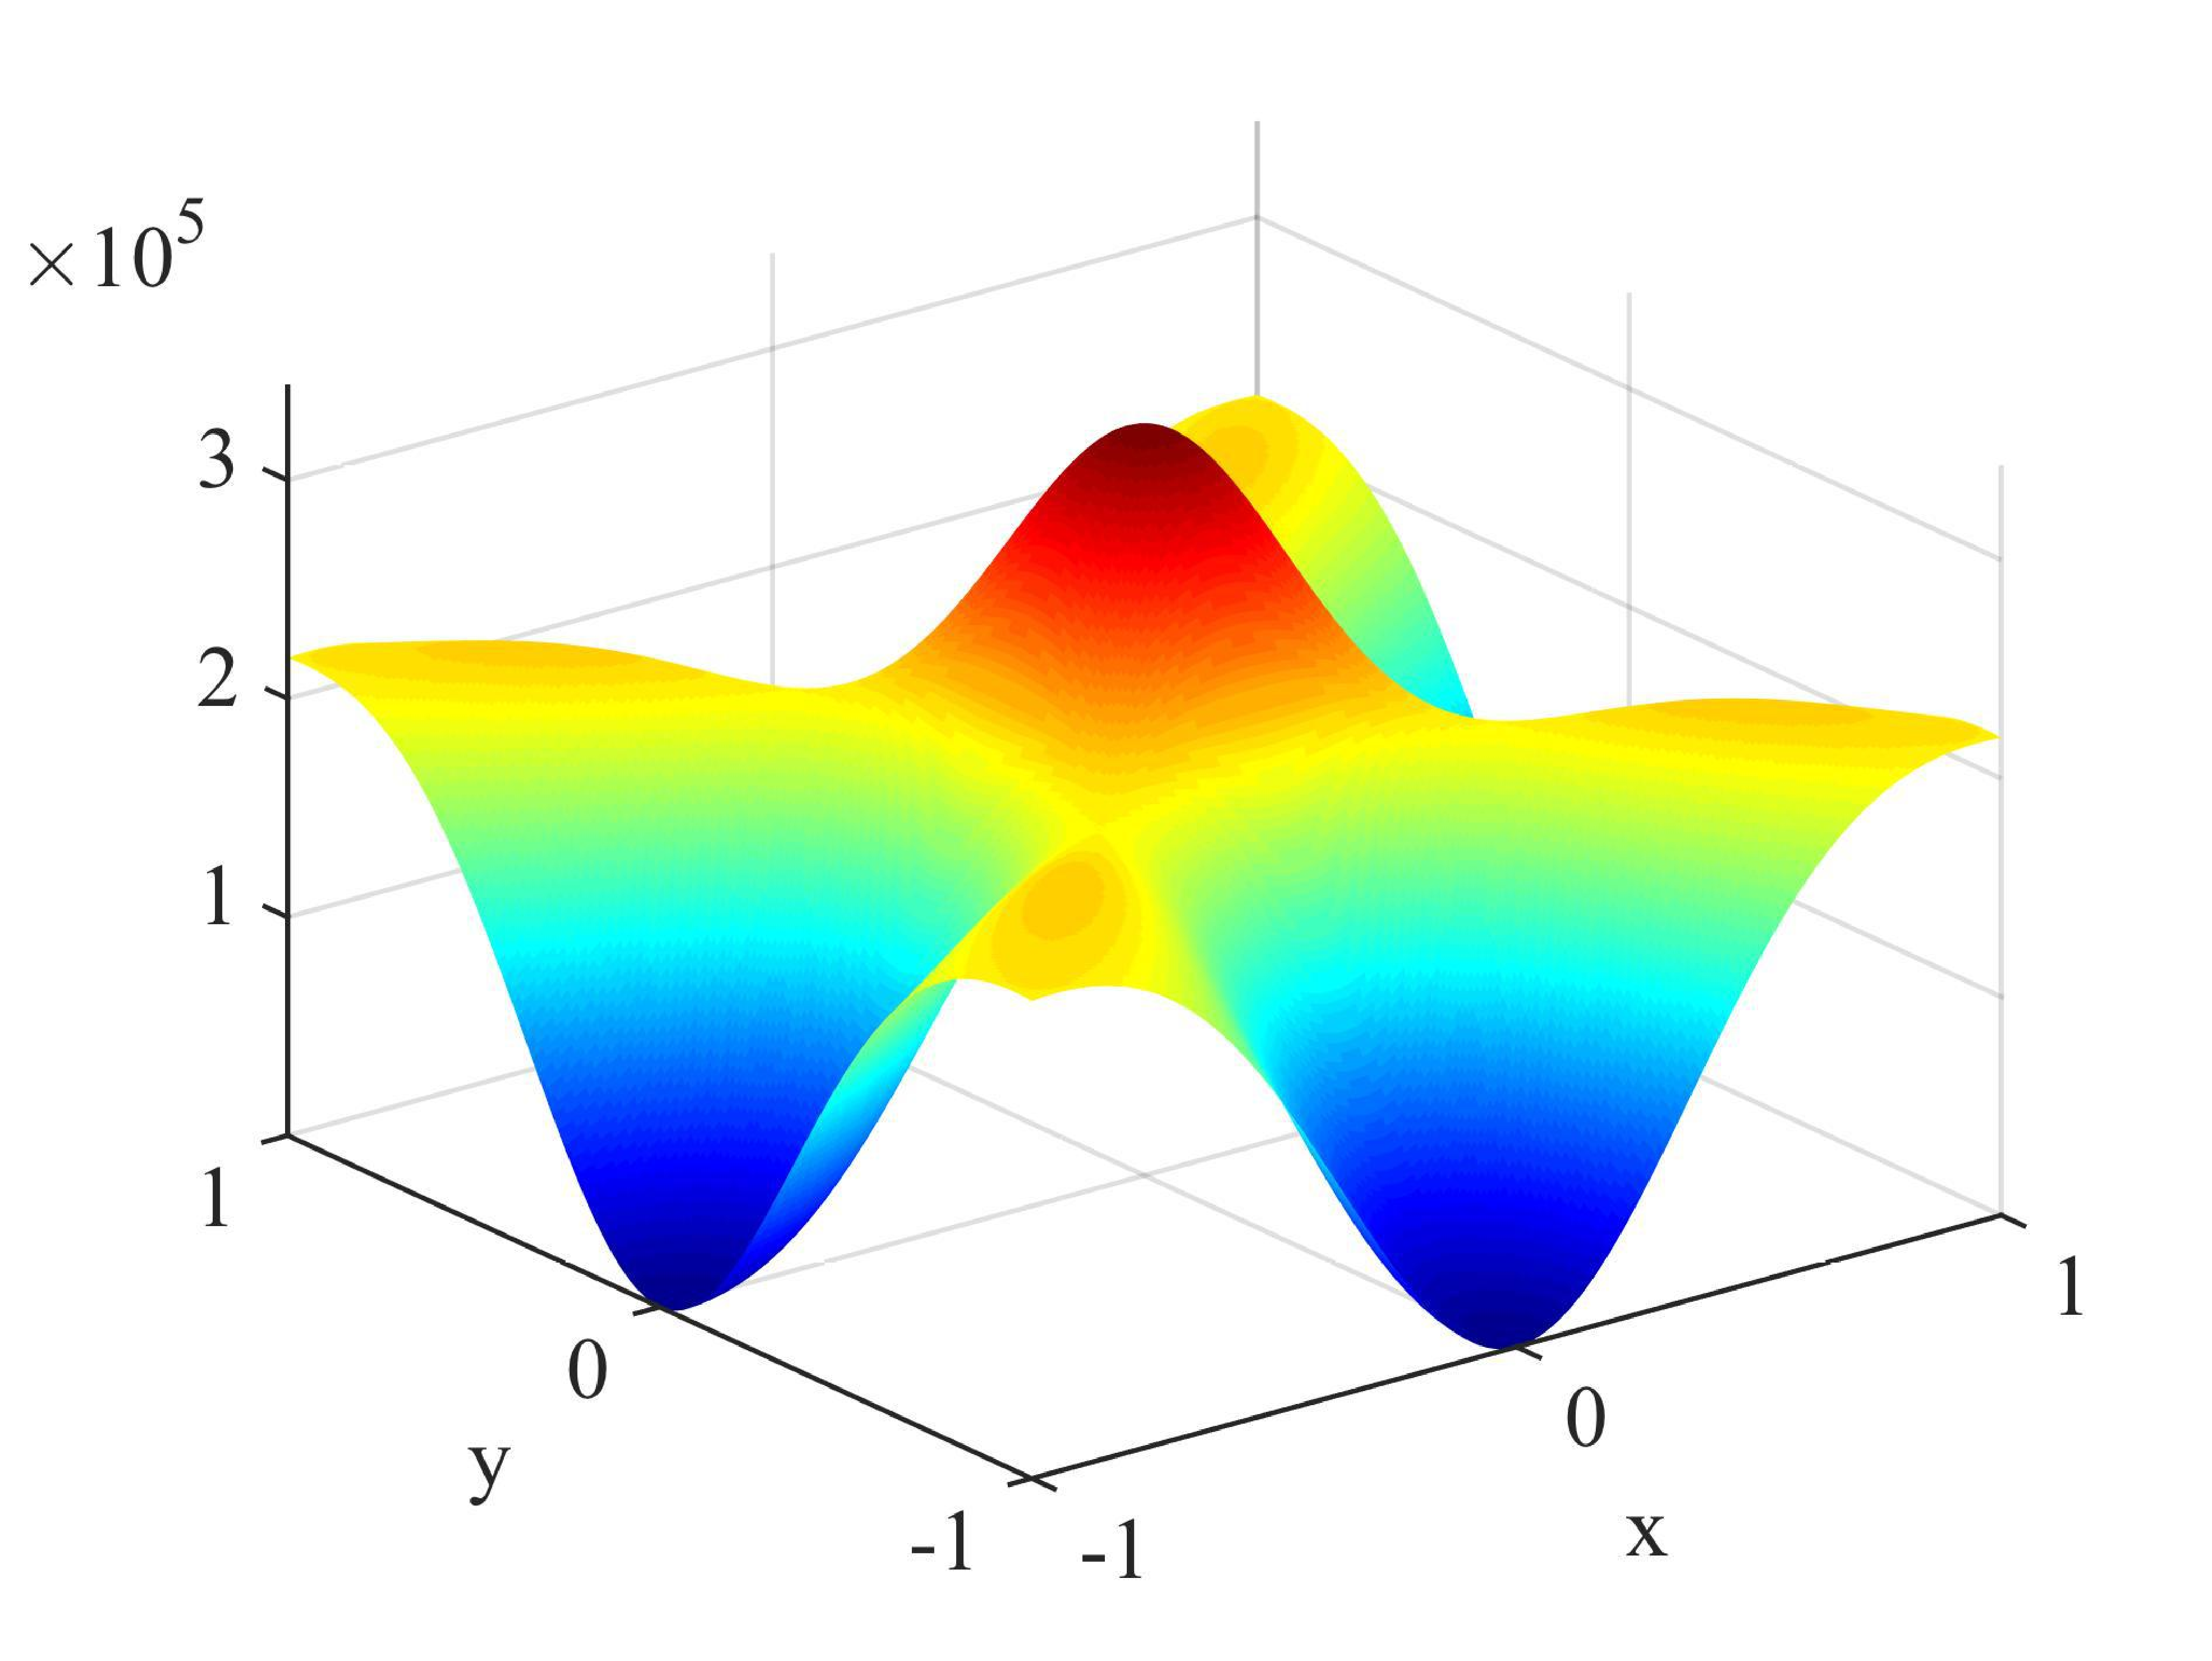
\includegraphics[width=0.45\textwidth]
   {figs/iso_shear_stereographic_detA.pdf}
 } \subfigure[Tangent]{
   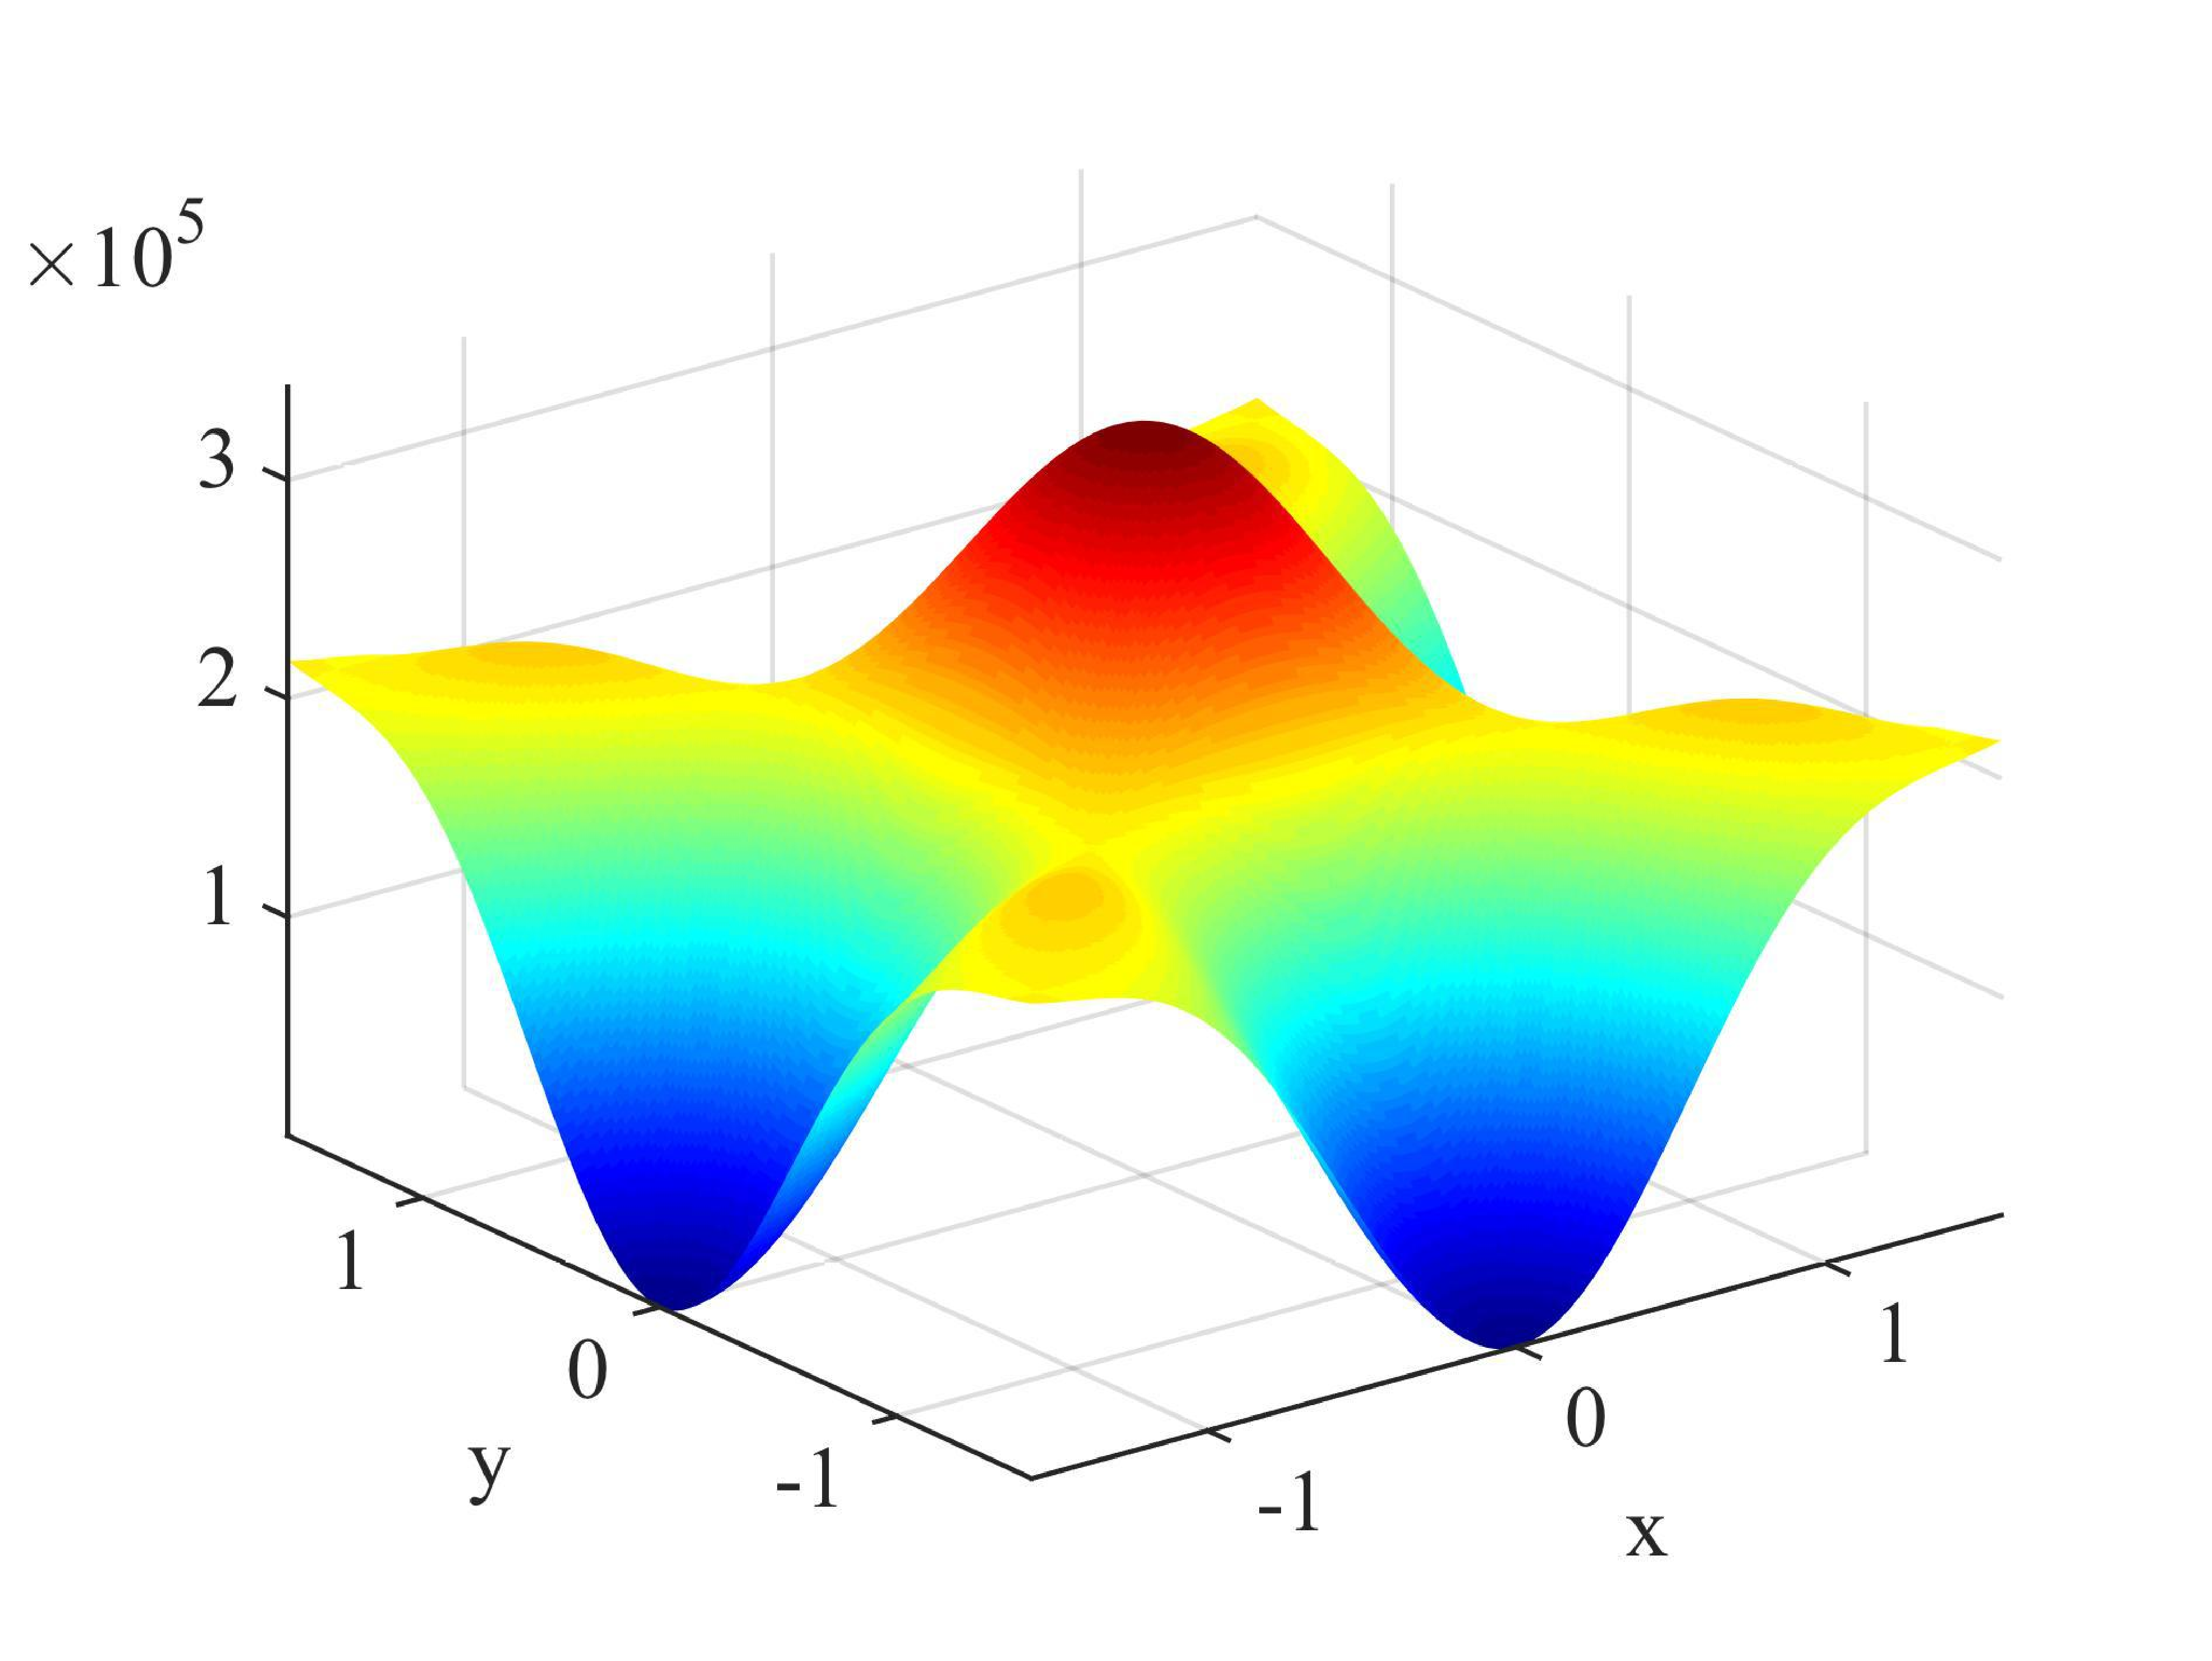
\includegraphics[width=0.45\textwidth]
   {figs/iso_shear_tangent_detA.pdf}
 }
   \caption{Landscapes of the determinant of the acoustic tensor at
     bifurcation for simple shear for the small deformation isotropic
     damage model.}
   \label{fig:iso-shear-detA}
 \end{figure}

\begin{figure}[!htbp]
   \centering \subfigure[Spherical]{
   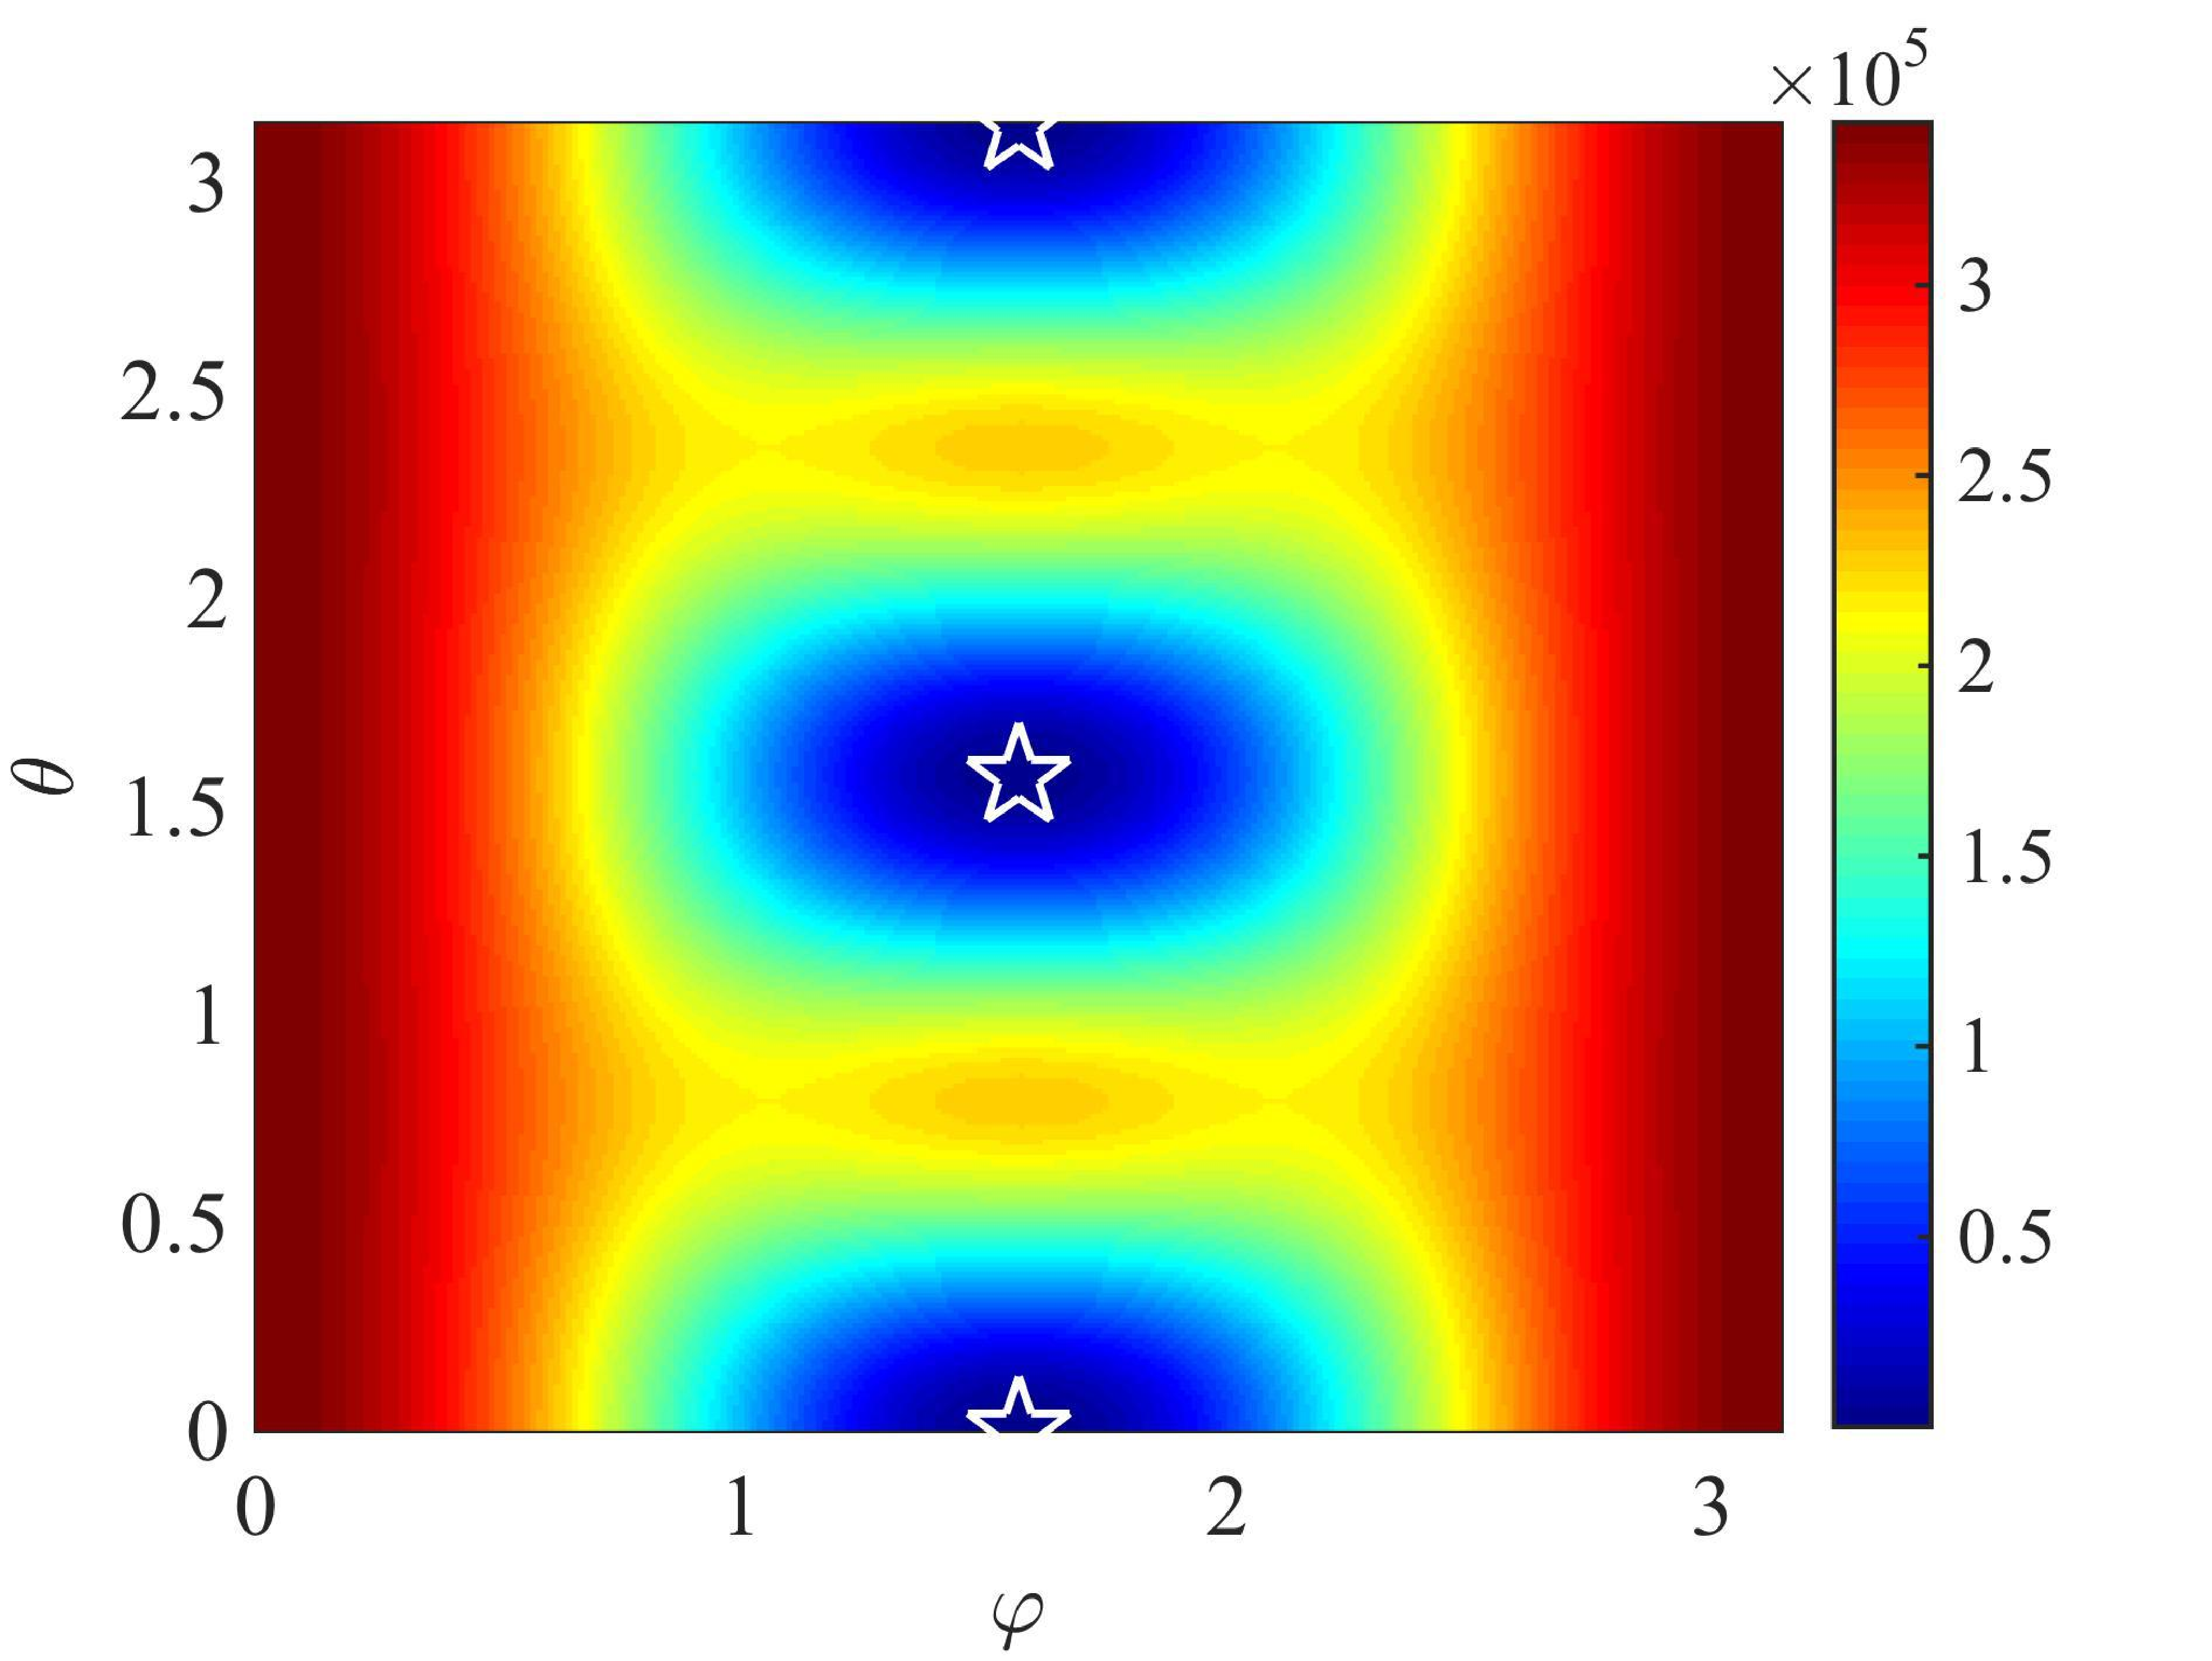
\includegraphics[width=0.45\textwidth]
   {figs/iso_shear_spherical_detAXplane.pdf}
 } \subfigure[Cartesian]{
   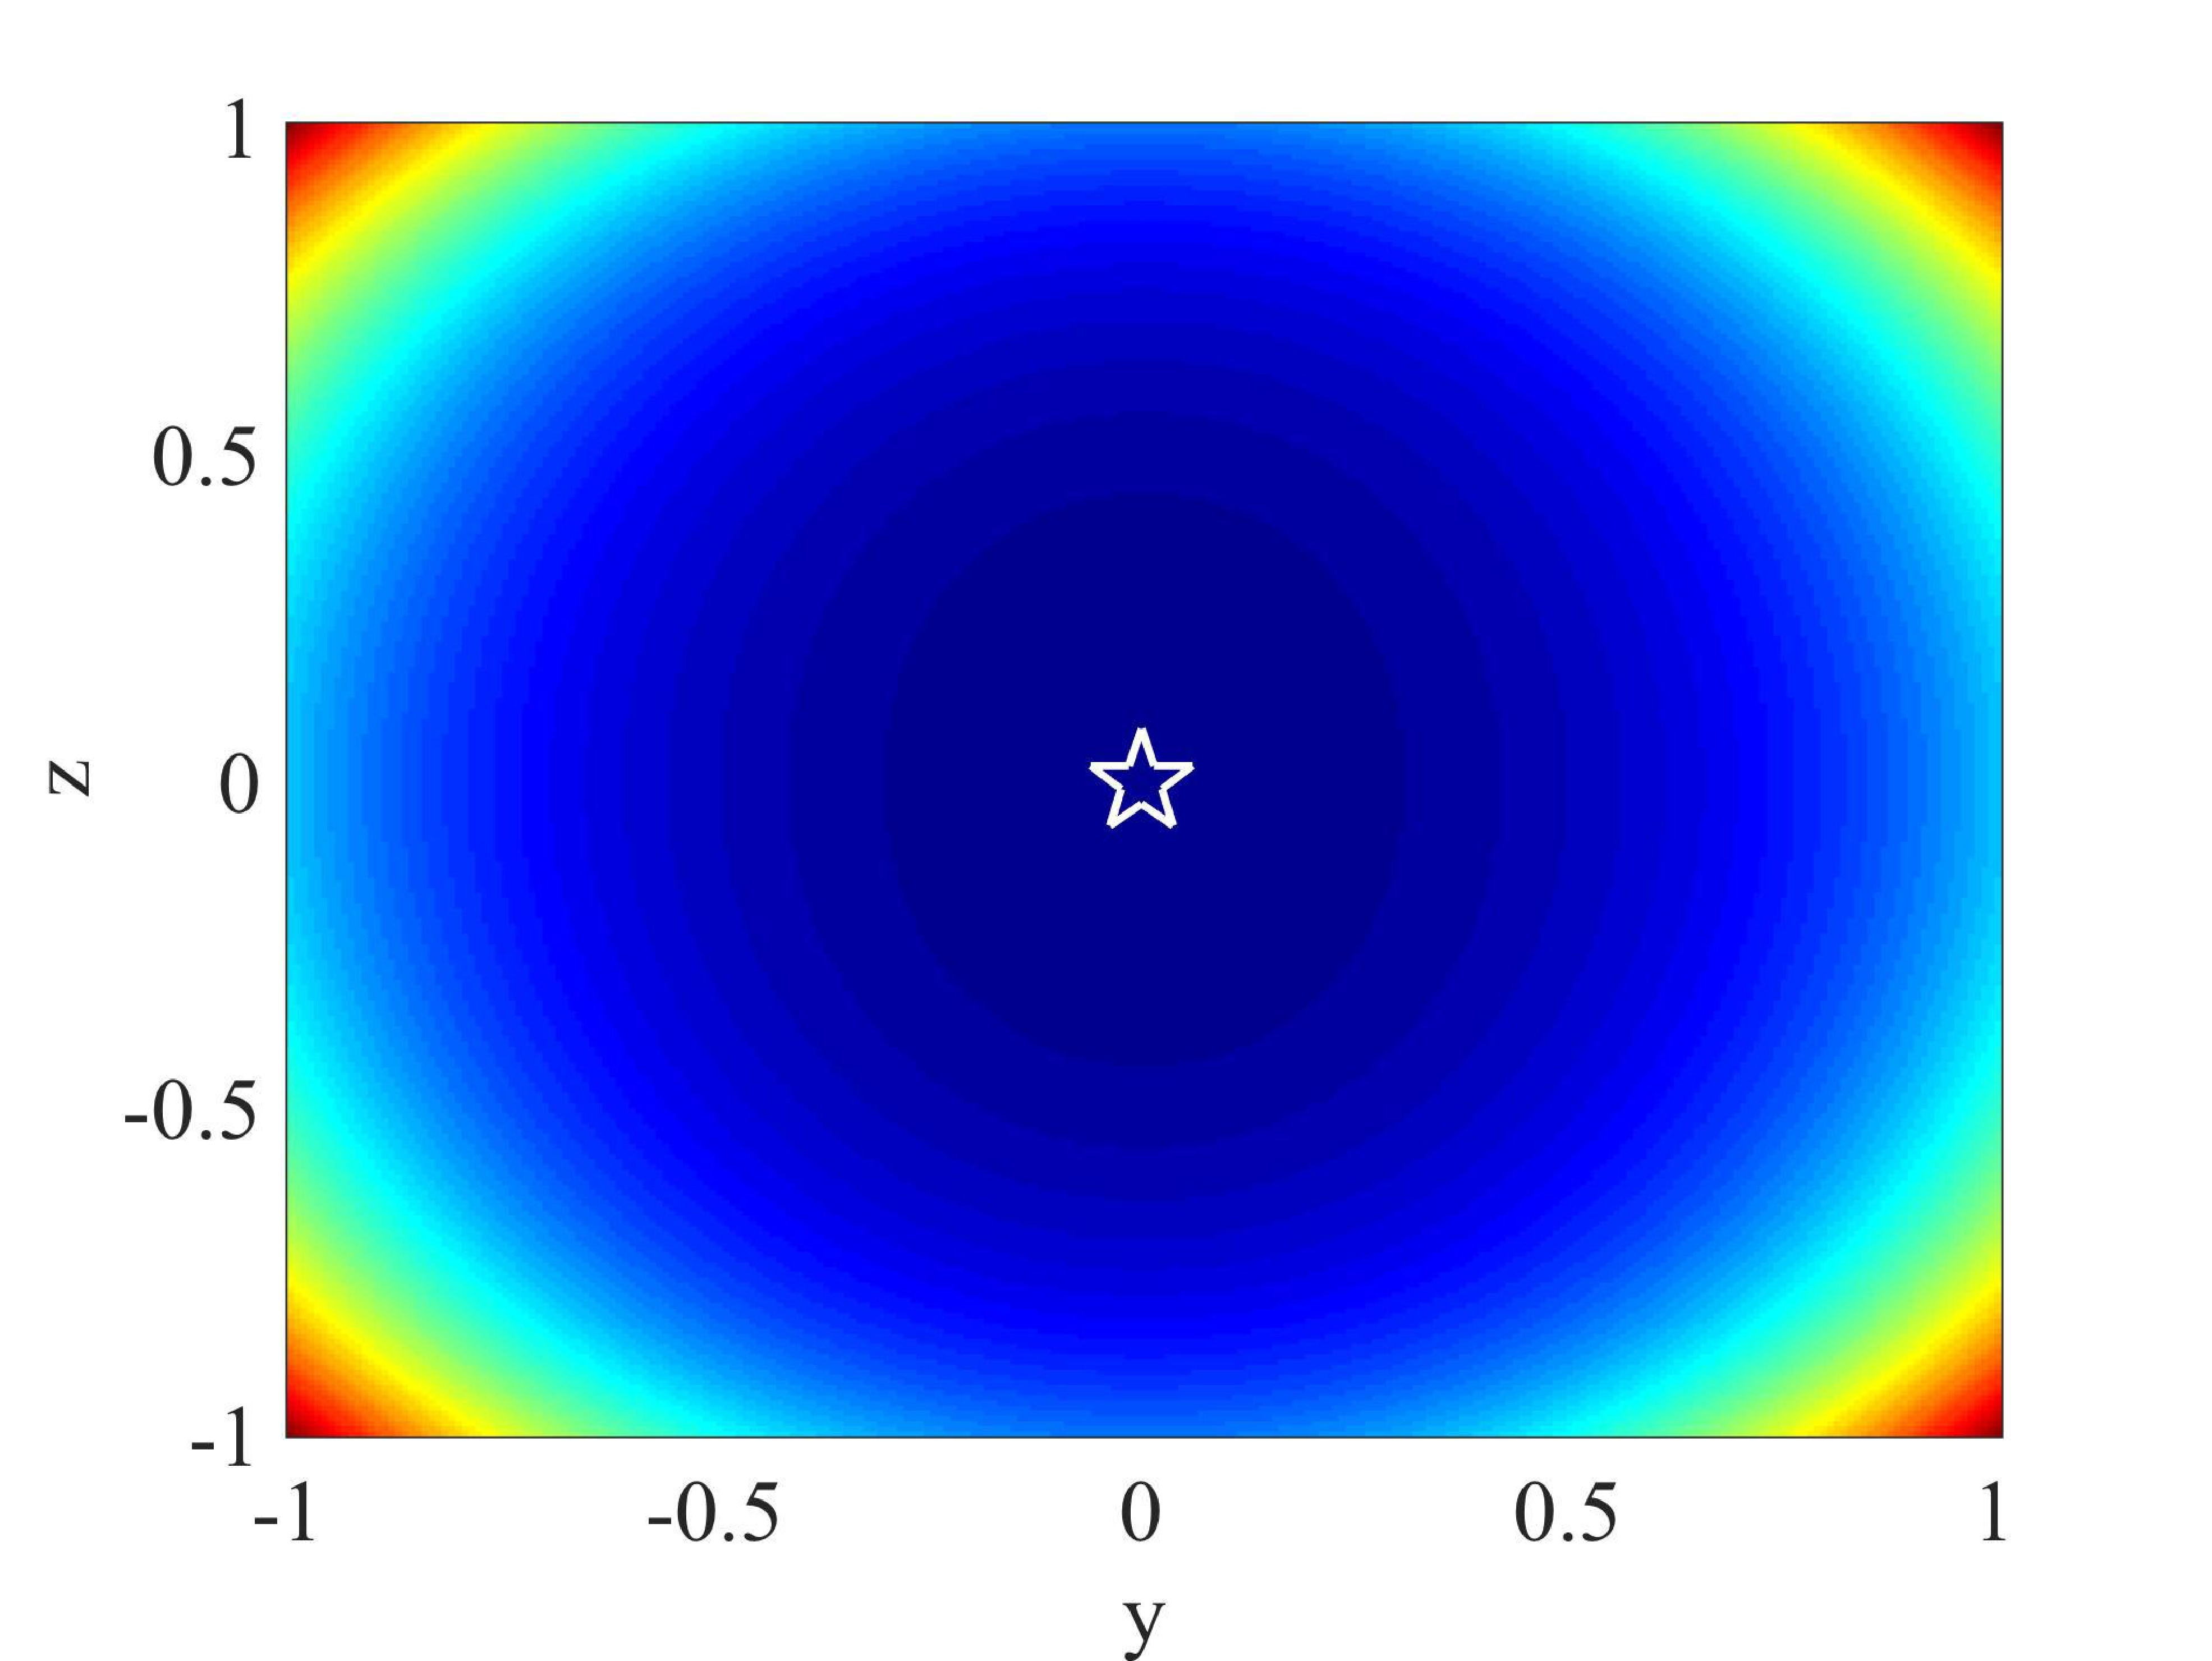
\includegraphics[width=0.45\textwidth]
   {figs/iso_shear_cartesian_detAXplane.pdf}
 } \subfigure[Stereographic]{
   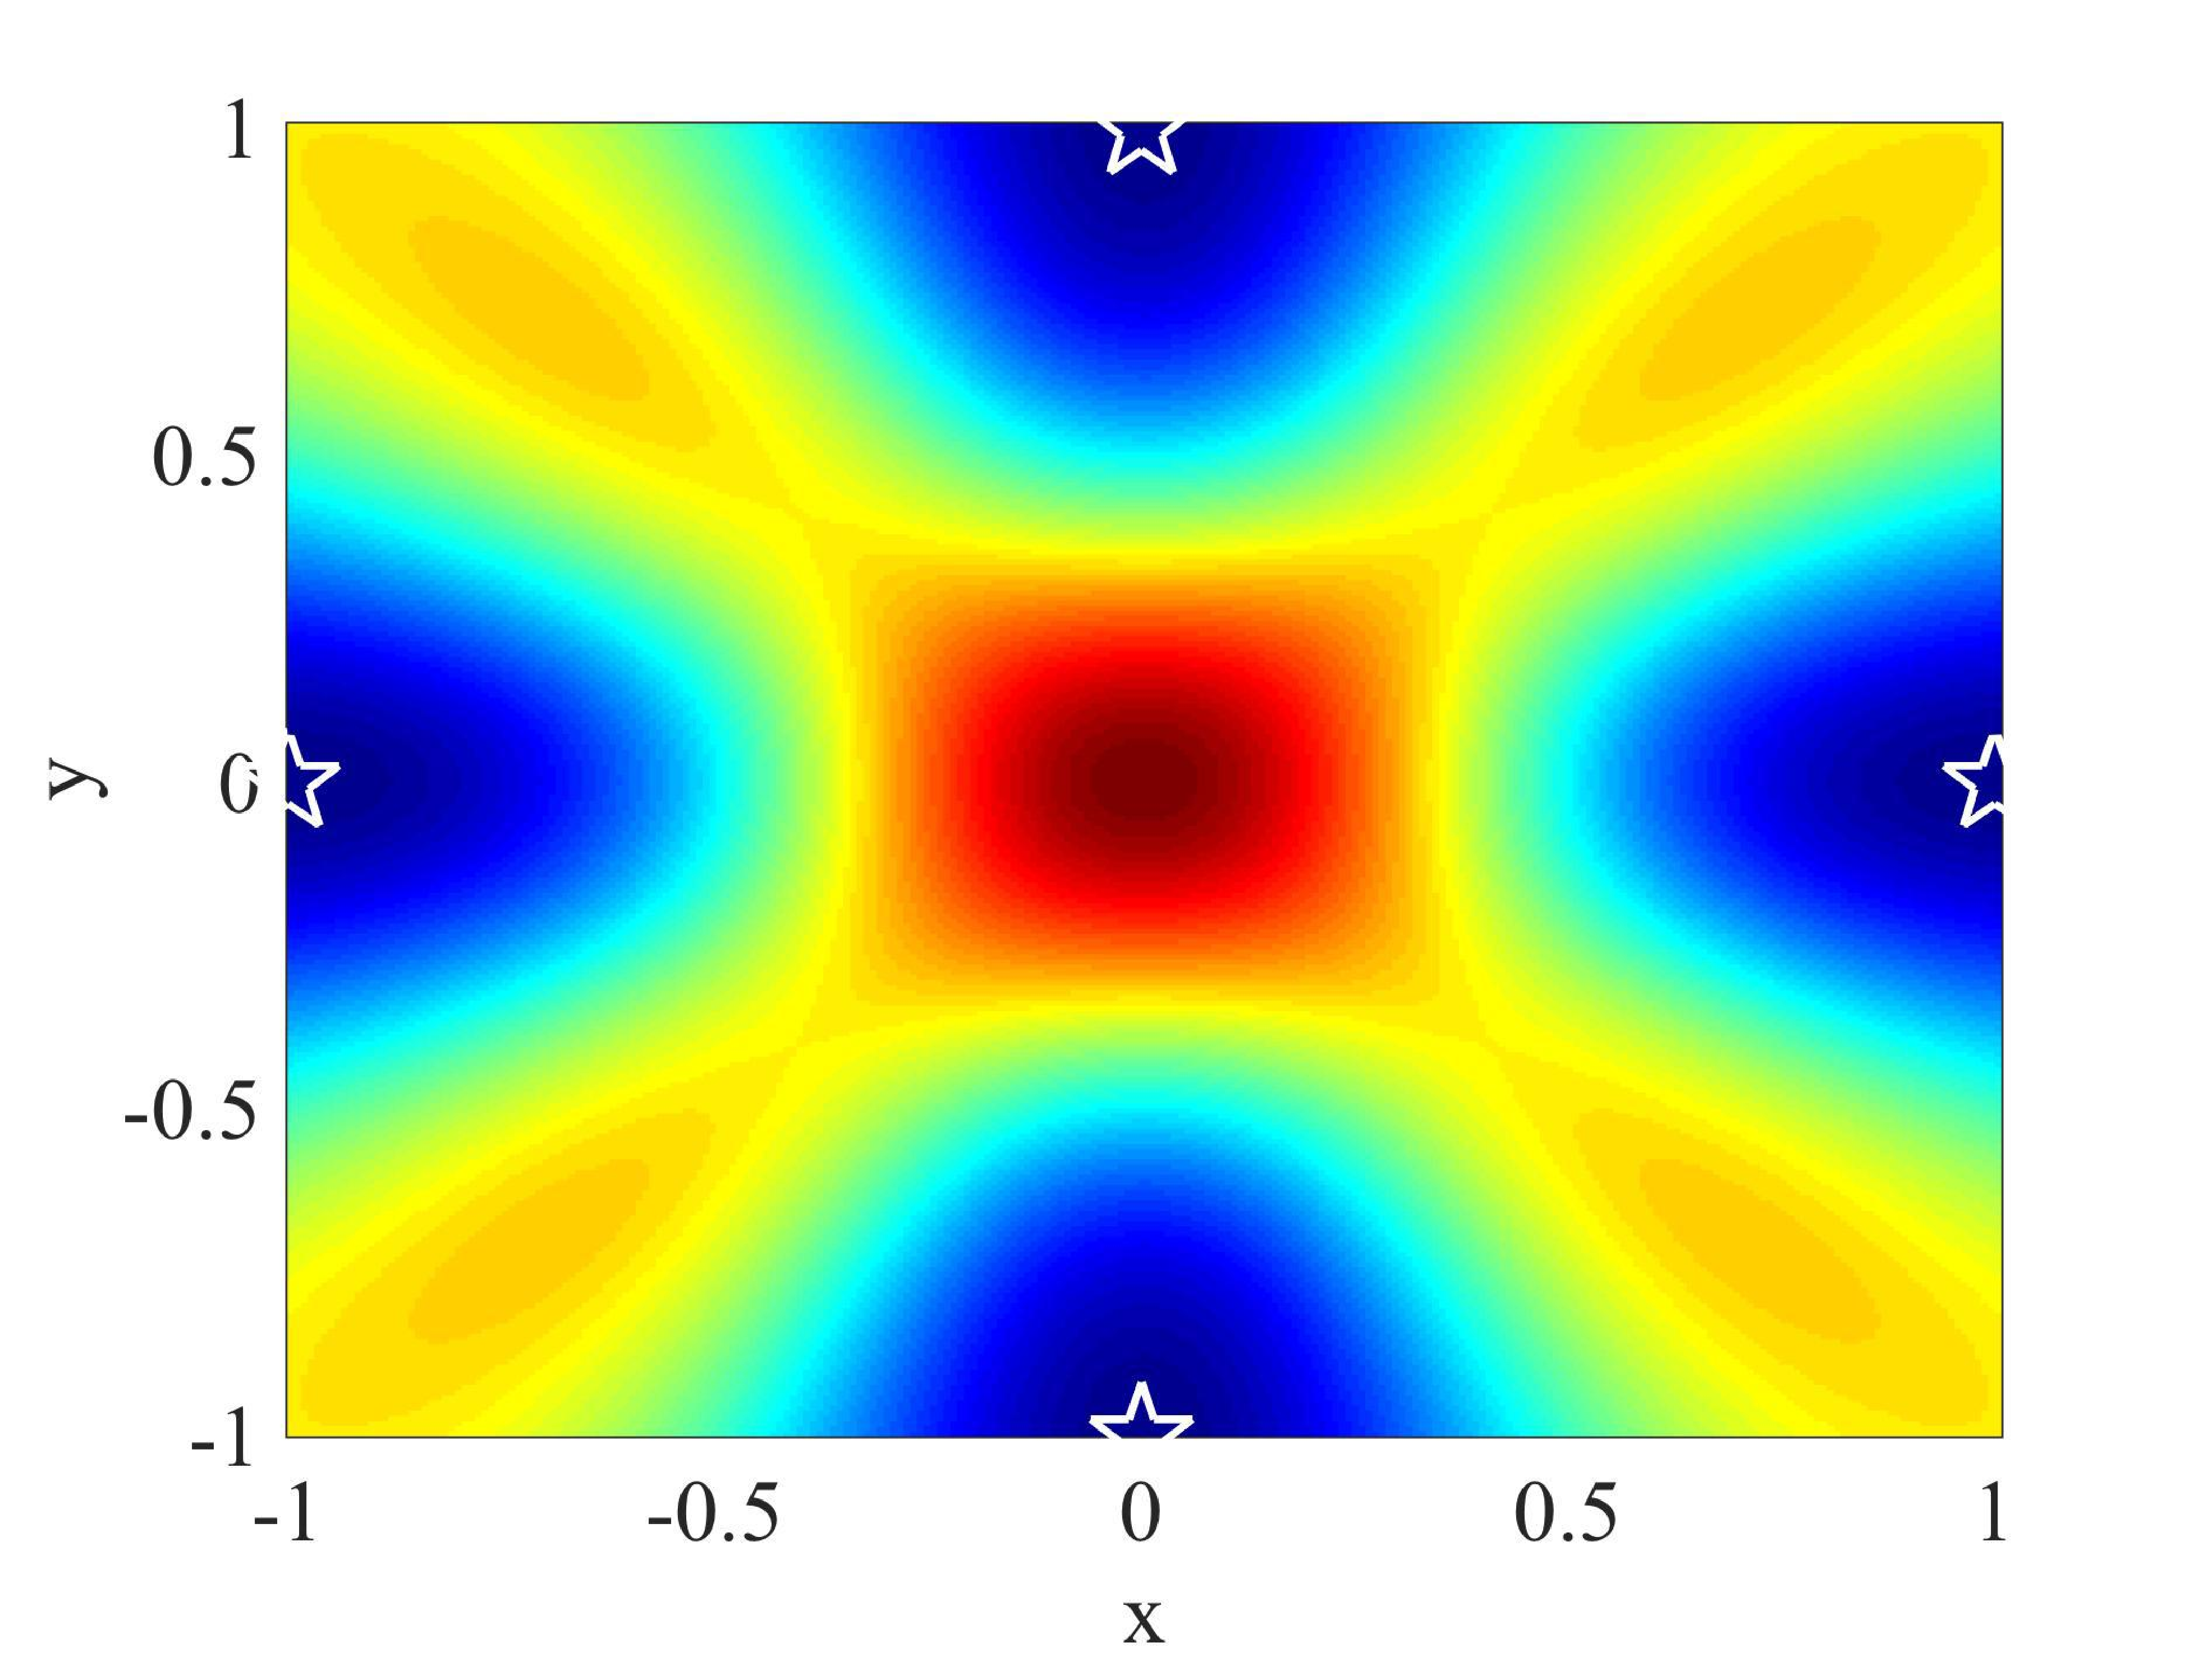
\includegraphics[width=0.45\textwidth]
   {figs/iso_shear_stereographic_detAXplane.pdf}
 } \subfigure[Tangent]{
   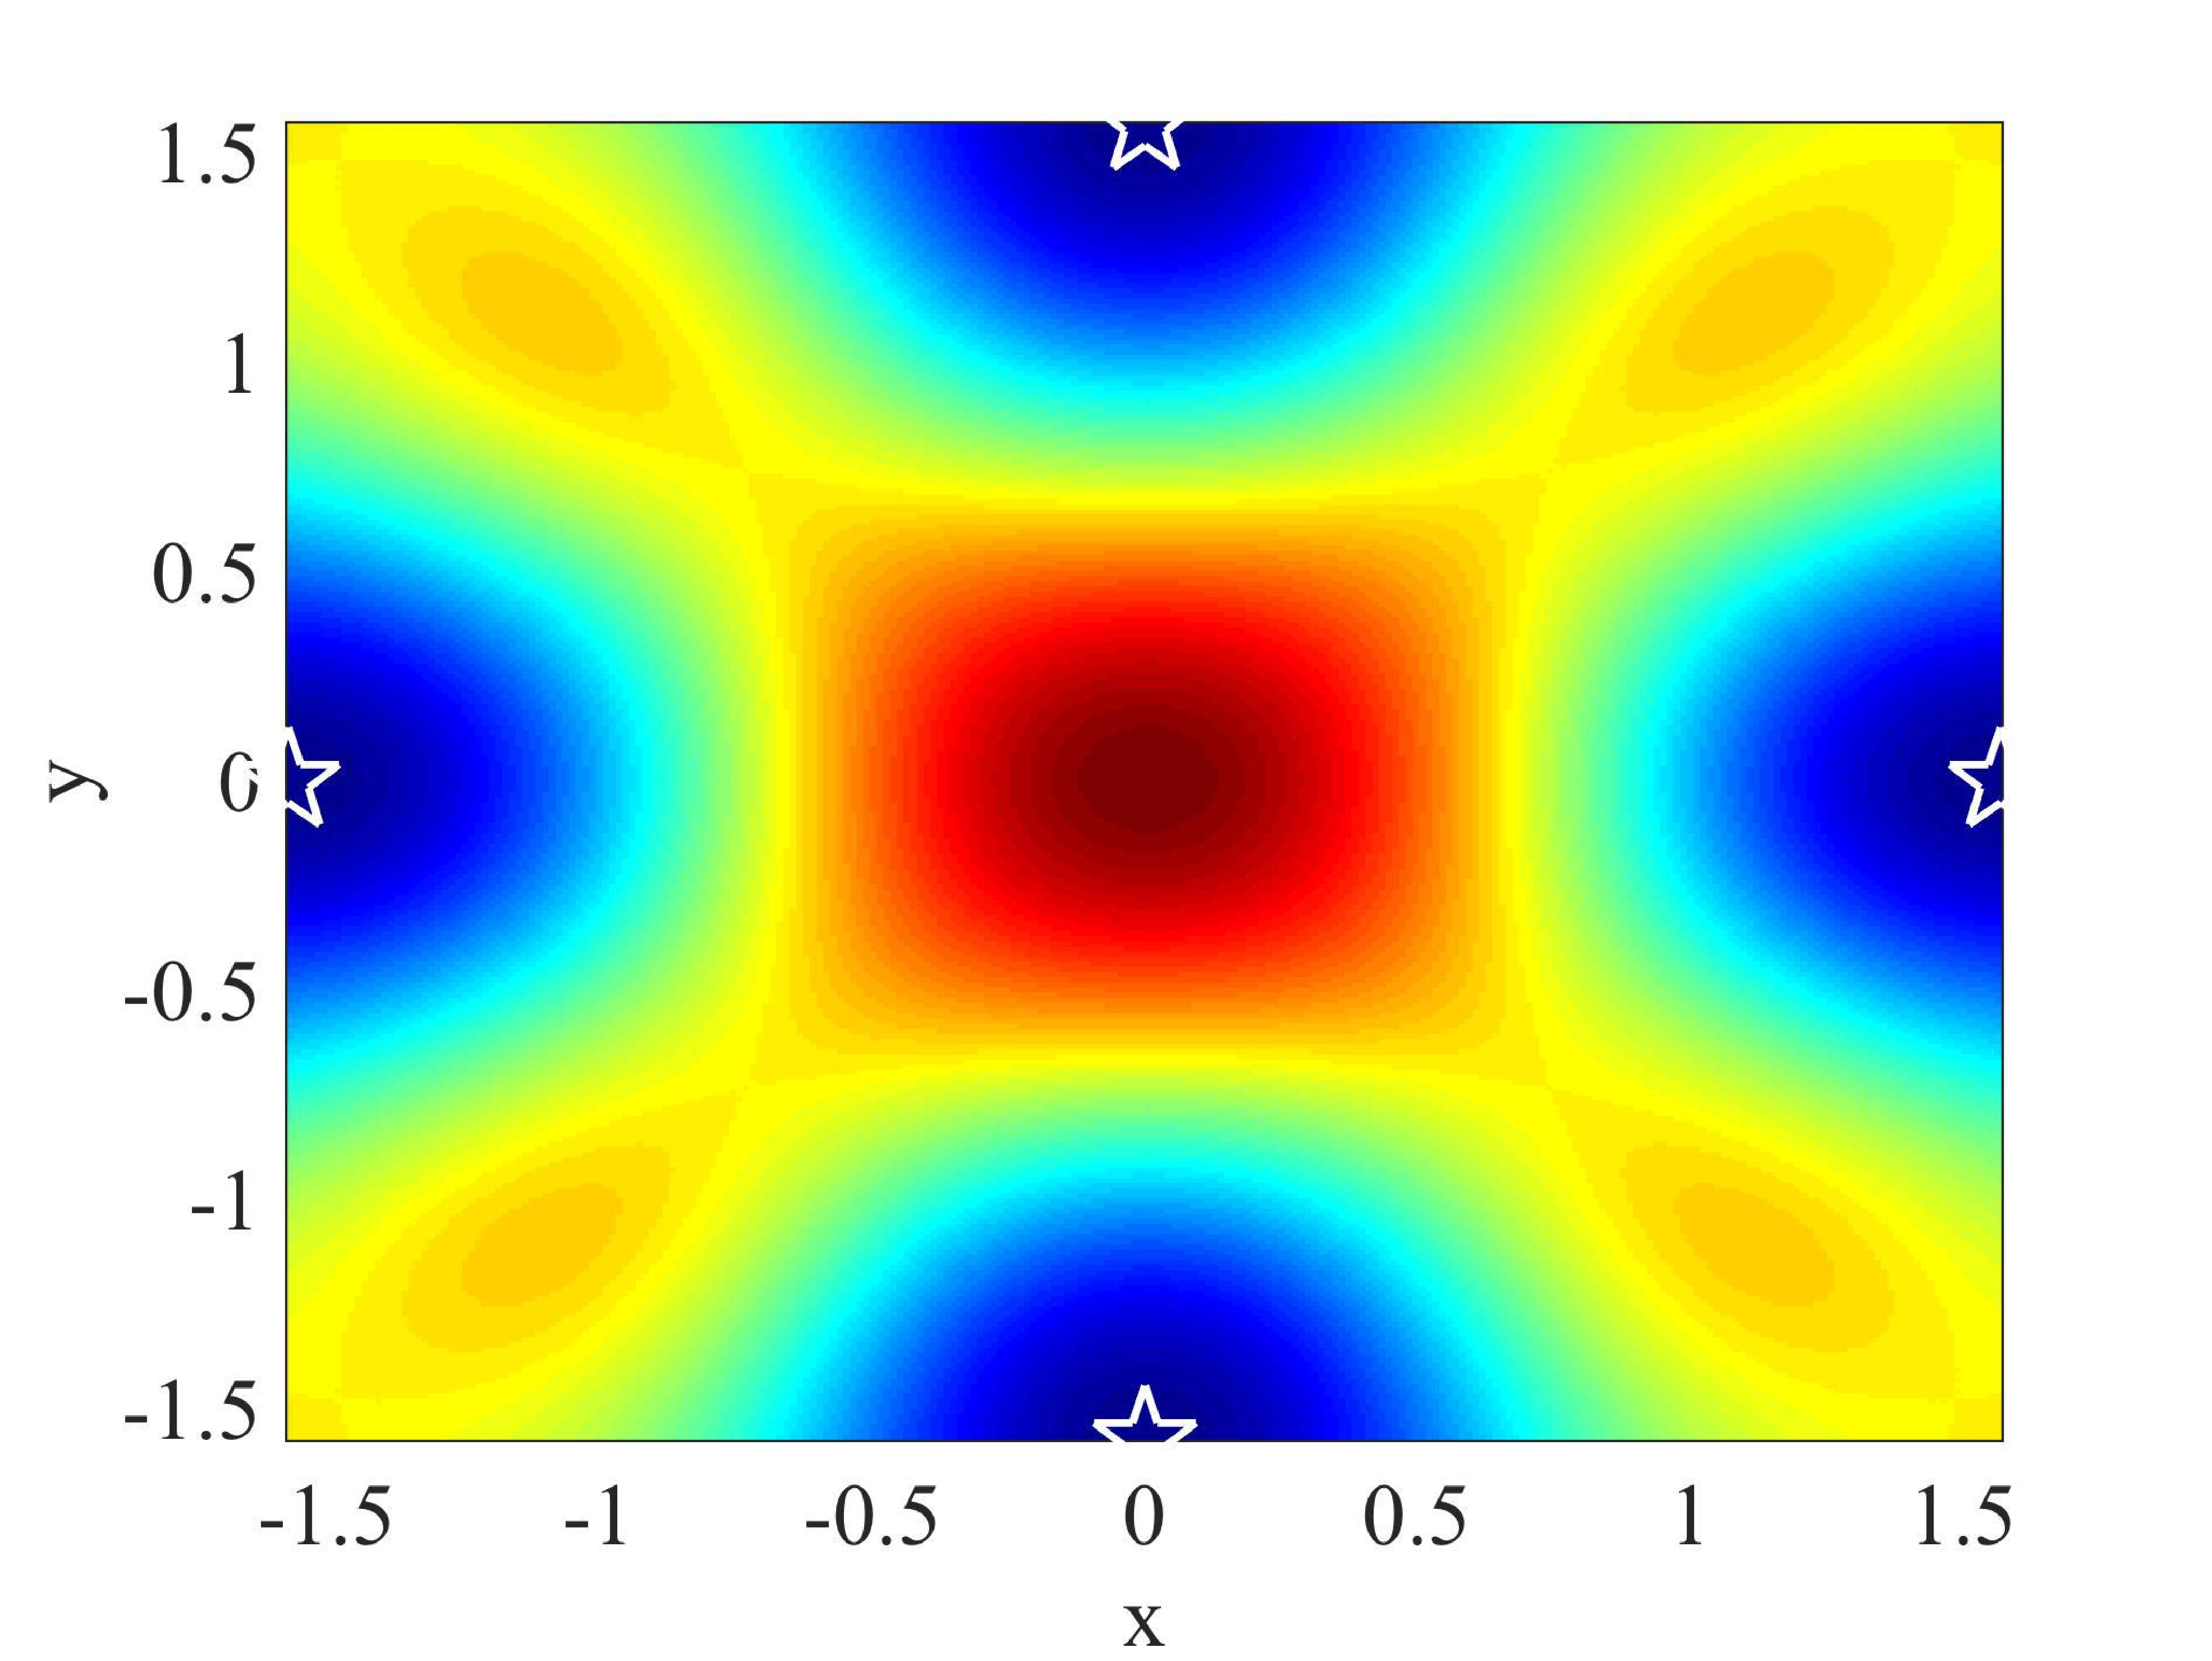
\includegraphics[width=0.45\textwidth]
   {figs/iso_shear_tangent_detAXplane.pdf}
 }
   \caption{Plane views of the landscapes of the determinant of the
     acoustic tensor at bifurcation for simple shear on the small
     deformation isotropic damage model. The white stars indicate
     global minima.}
   \label{fig:iso-shear-detAXplane}
 \end{figure}

It is clear from these landscape plots that the complexity of the
shape of the determinant function depends greatly on the choice of
parametrization. Even for the very simple small deformation isotropic
model adopted in this example, the landscape of the determinant
function can be quite complex as in the cases of the spherical,
stereographic and tangent parametrizations.

The Cartesian parametrization results in a simple bowl-shaped
objective function, which renders the Newton iterative scheme to be
particularly robust and insensitive to the initial guess. Evidence for
this can be seen in Table~\ref{tab:iso-shear-runtime} as the
Cartiesian and spherical parametrizations are the only ones able to
detect bifurcation when the sampling grid is reduced to a single
point.

We now elaborate further on the robustness of the parametrizations by
considering the situation in which the initial sampling is eliminated
altogether. In the absence of the initial sampling, a random point
within the corresponding parametric space is provided as initial guess
for the Newton iterative scheme when $\epsilon_{12}=0.0559$, \ie, at
the onset of bifurcation. If Algorithm~\ref{alg:adaptive-step} is able
to correctly detect the onset of bifurcation and its associated
directions, the parametrization is said to succeed for this one set of
randomly generated parameters. This process is repeated 1000 times for
each parametrization.

Table~\ref{tab:iso-shear-random-para} shows the rate of successful
bifurcation detection for all five parametrizations. The average
number of iterations and the computation time of those successful
detections are also recorded and shown in the table. It can be seen
that the proposed Cartesian parametrization is much more robust than
the commonly used spherical parametrization, \cf $100\%$ \vs $12.8\%$
success rate. Furthermore, the Cartesian parametrization also
outperforms the remaining three parametrizations. In term of
computational cost, the Cartesian paramtrization is also efficient
with an average run time of $207\mu\text{s}$.

\begin{table}[!htbp]
  \begin{center}
    \begin{tabular}{l | c c c c c}
      \toprule
      & Spherical & Stereographic & Projective & Tangent & Cartesian \\
      \midrule
      Success rate ($\%$)      & 12.8 & 22.7 & 59.9  & 20.6  & 100   \\
      Average iteration count    & 4.39 & 4.70 & 8.86  & 5.12  & 5.35   \\
      Average run time (${\mu\text{s}}$) & 211  & 242  & 495  & 264  & 207 \\
      \bottomrule
    \end{tabular}
    \caption{Isotropic small deformation model: success rate and
      computational cost of Newton iterative scheme with a single
      random initial point. A total of 1000 random trials are
      performed for each parametrization.}
    \label{tab:iso-shear-random-para}
  \end{center}
\end{table}

The better performance of the proposed Cartesian parametrization in
terms of computational efficiency and robustness can be attributed to
its relatively simple determinant function landscape.
\fref{fig:iso-shear-robust} shows contours of the determinant
functions corresponding to Table~\ref{tab:iso-shear-random-para}. One
thousand random initial points are also plotted. If the initial guess
leads to a successful detection of bifurcation and its directions, the
point is marked as a solid circle ($\bullet$). Otherwise, it is marked
as a cross ($\times$). This figure provides a very direct
visualization of the robustness results.

\begin{figure}[!htbp]
   \centering \subfigure[Spherical]{
   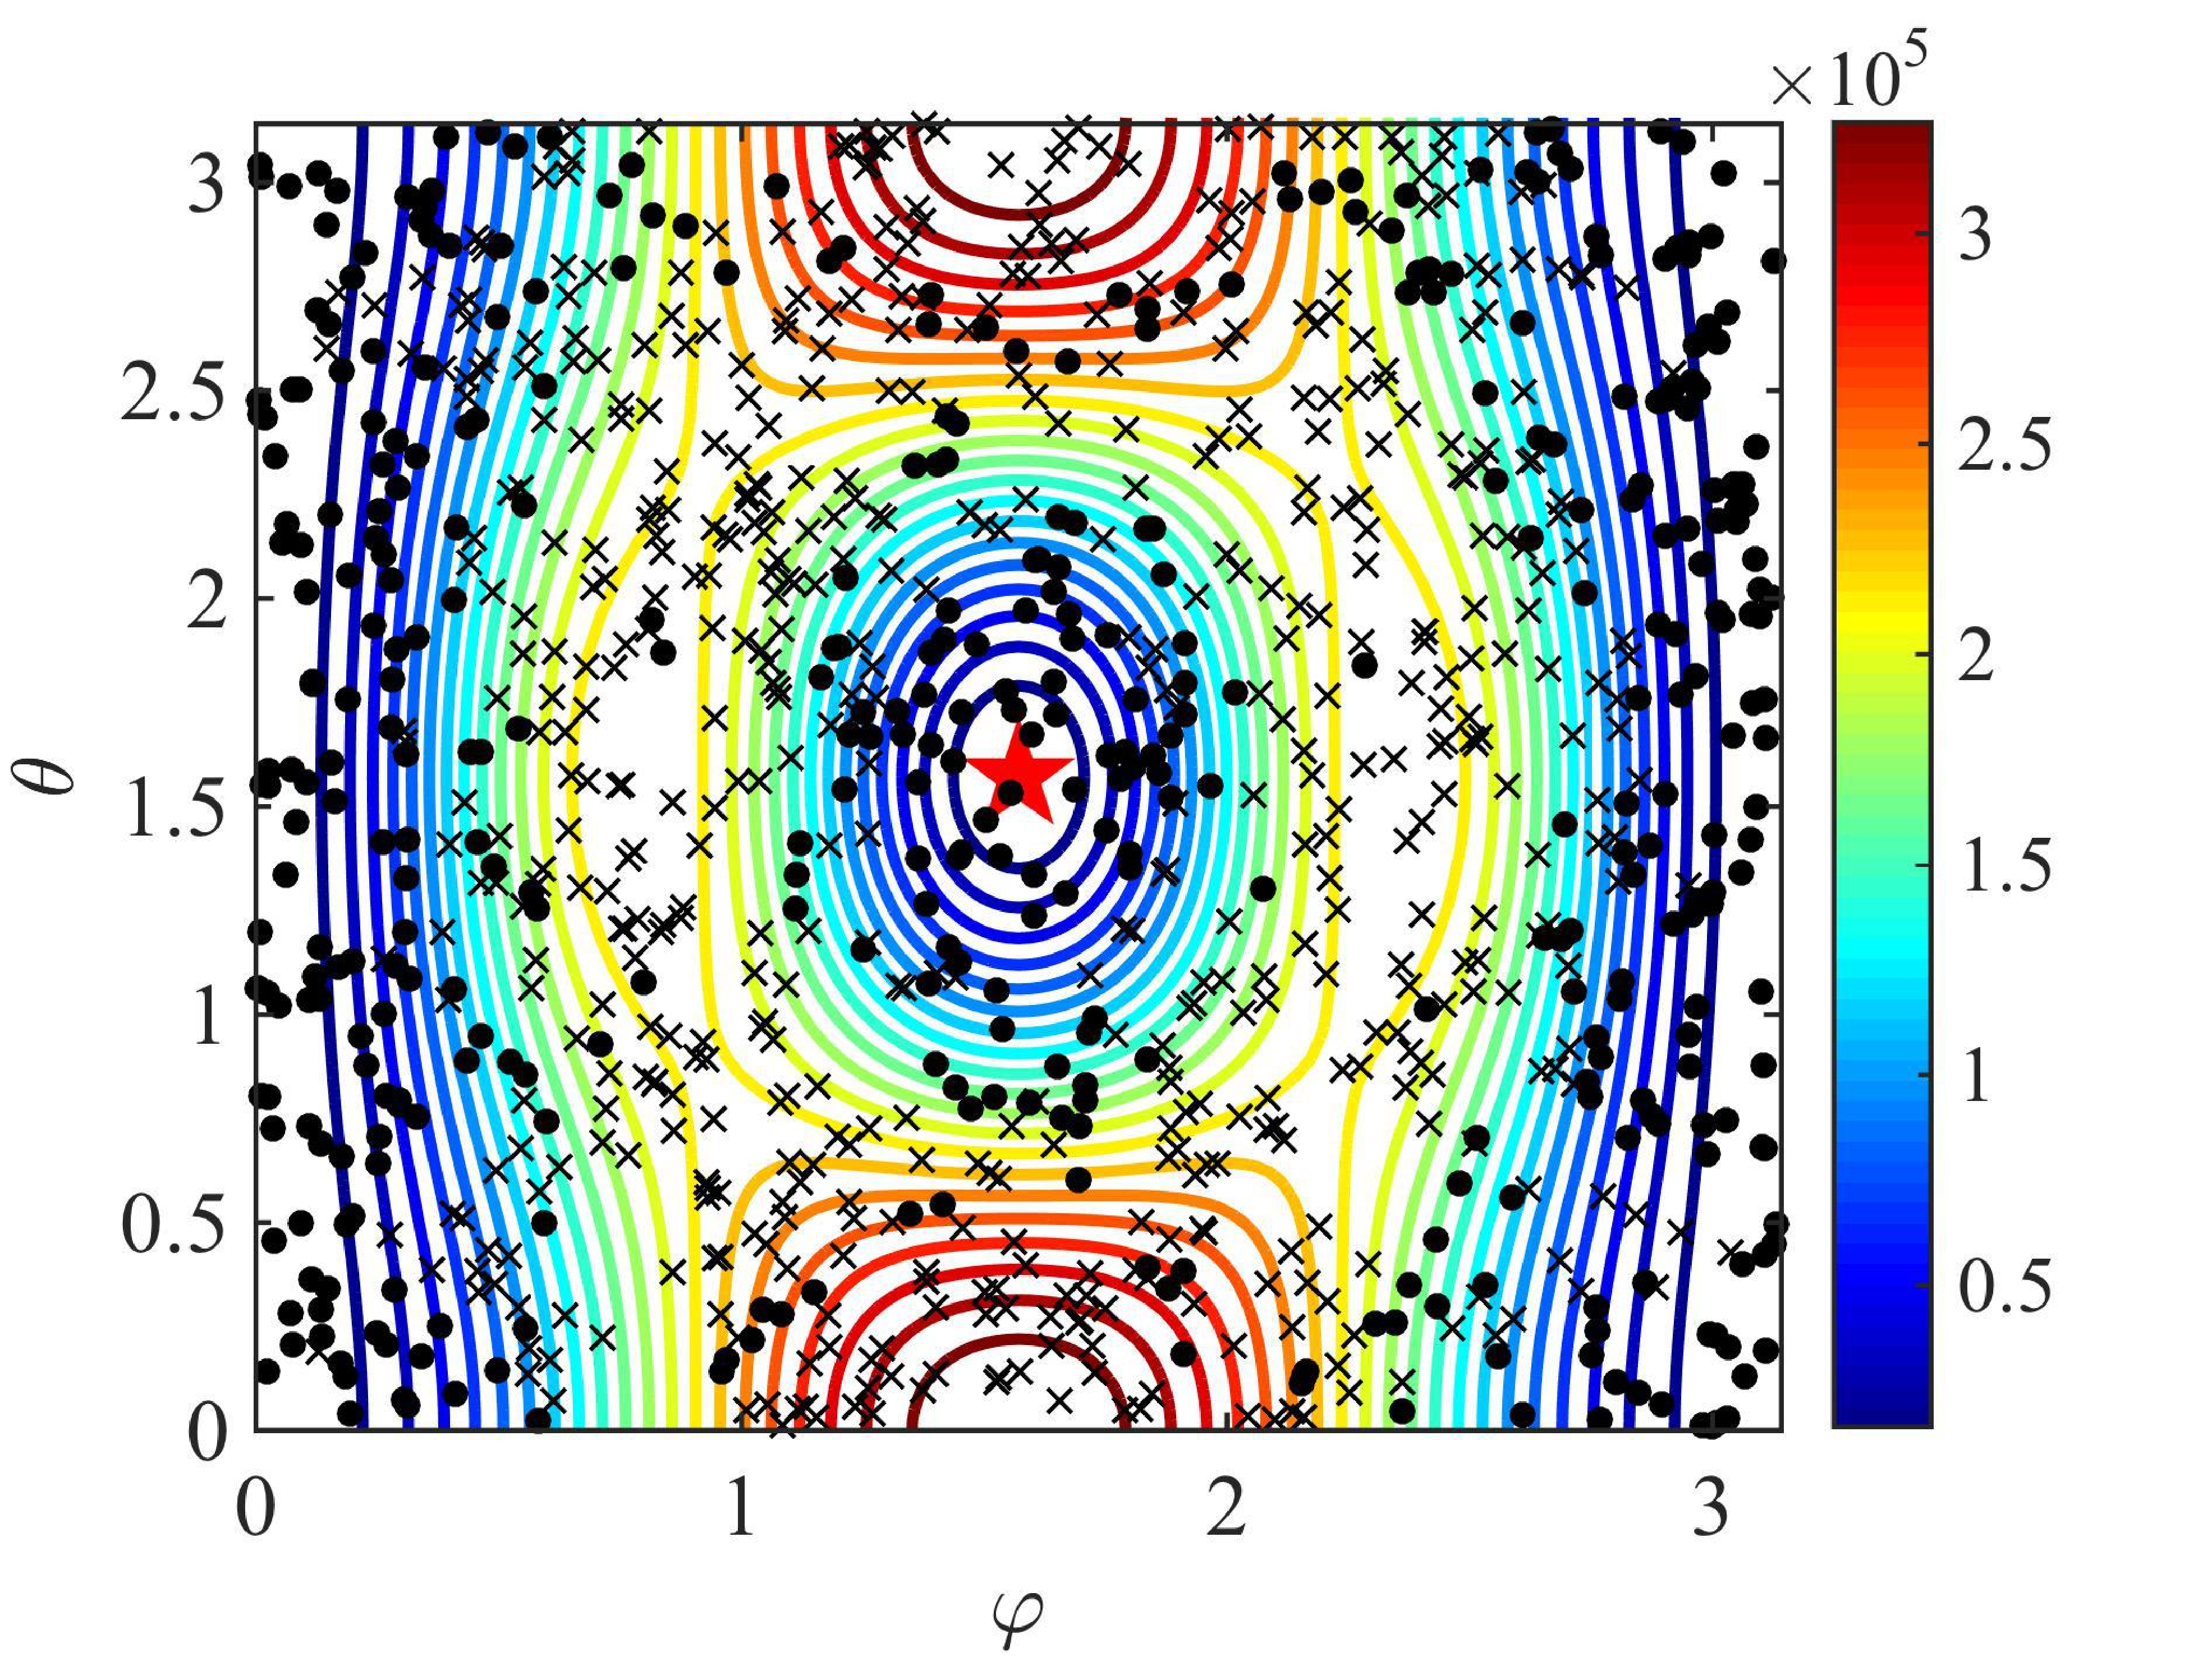
\includegraphics[width=0.47\textwidth]
   {figs/iso_shear_spherical_random.pdf}
 } \subfigure[Cartesian]{
   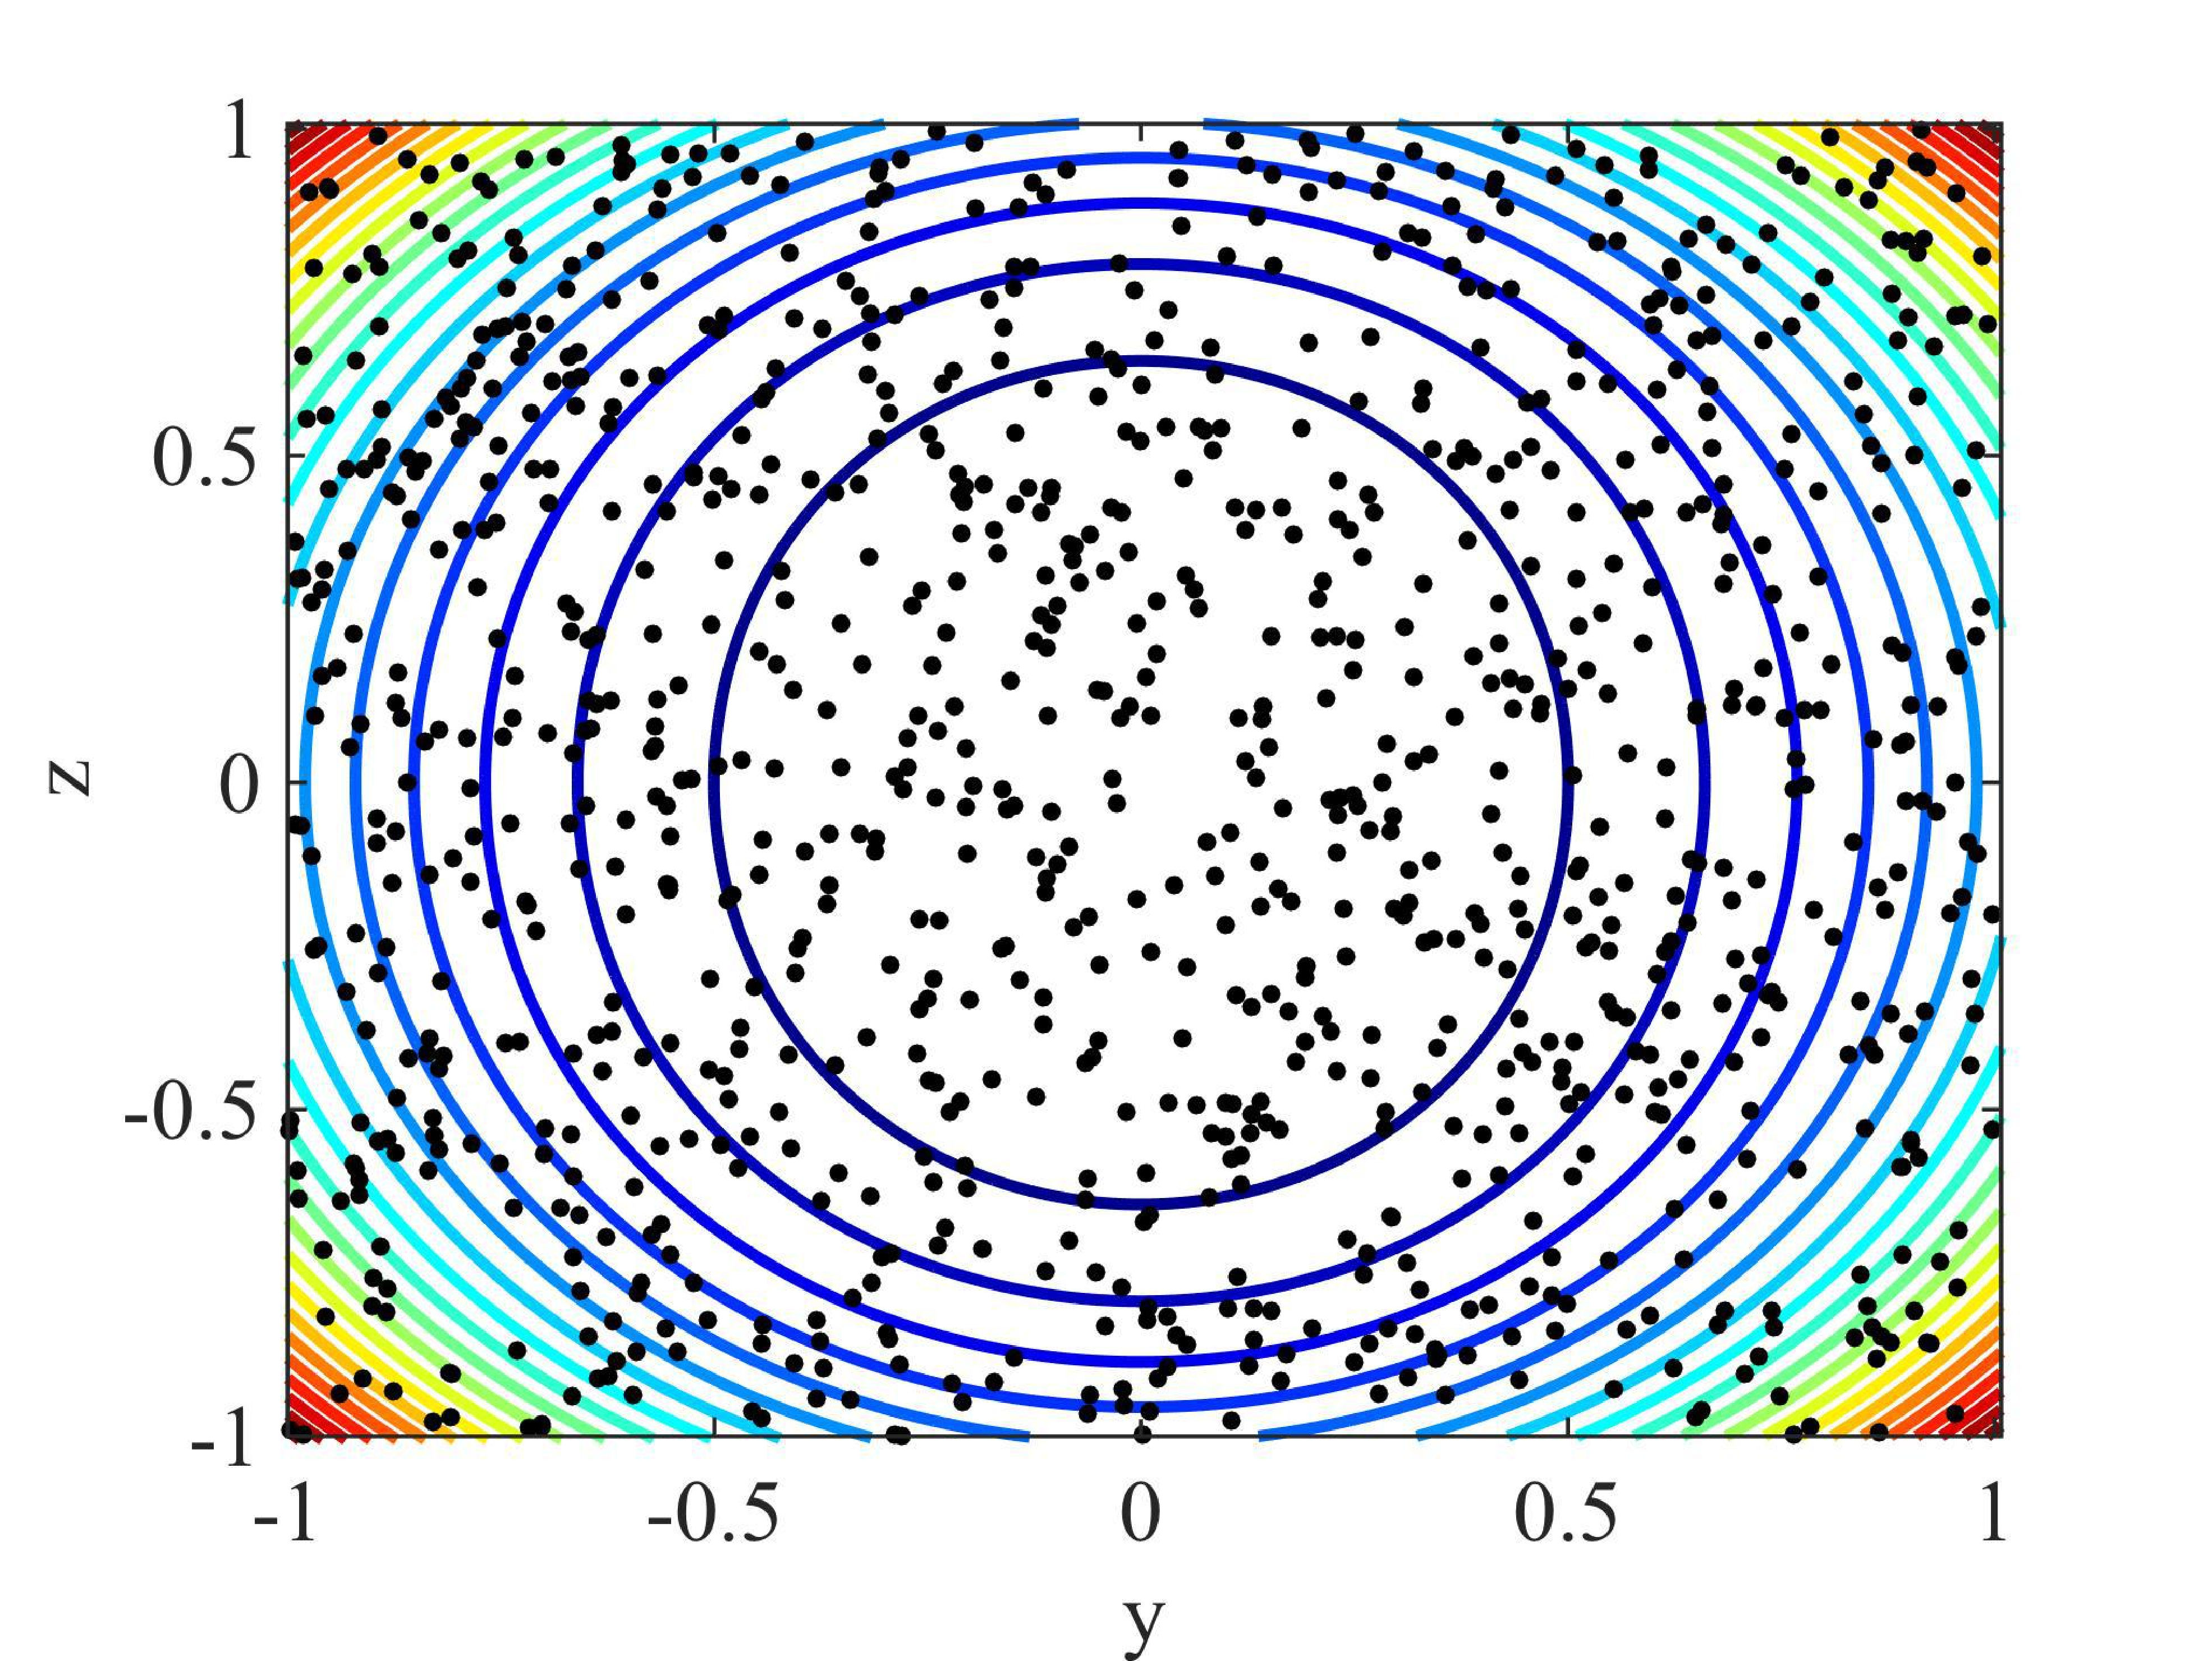
\includegraphics[width=0.47\textwidth]
   {figs/iso_shear_cartesian_random.pdf}
 } \subfigure[Stereographic]{
   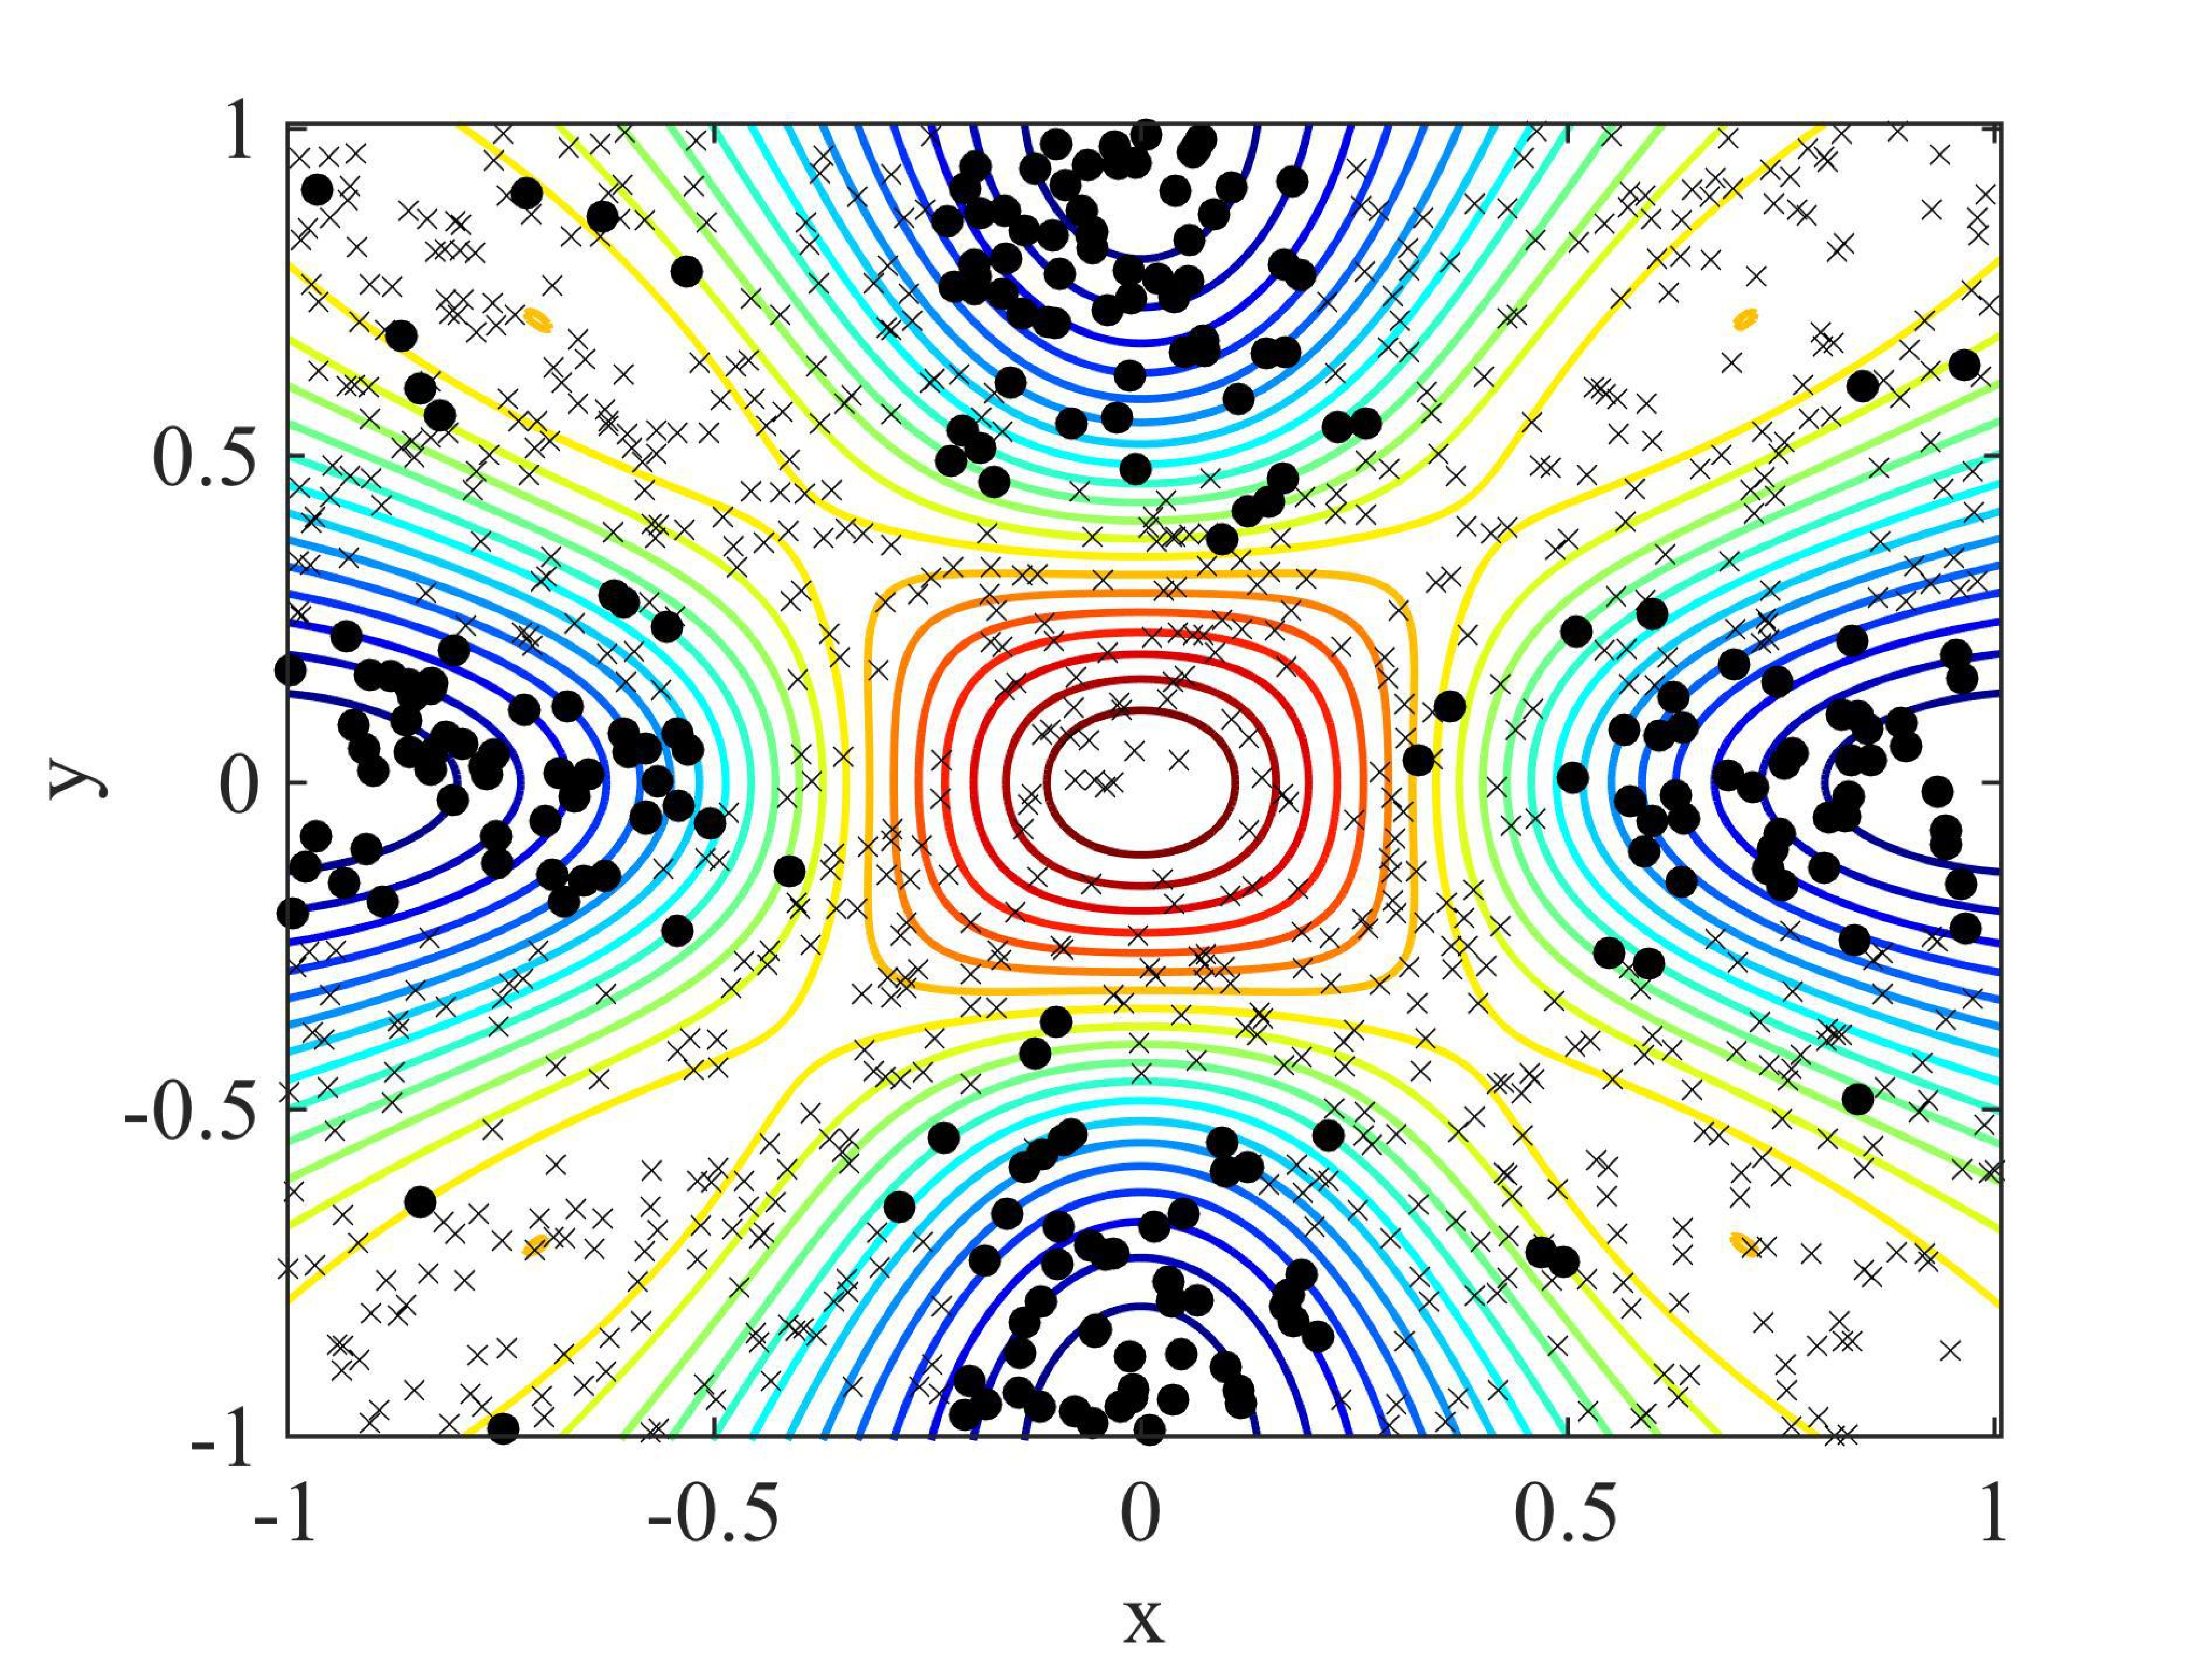
\includegraphics[width=0.47\textwidth]
   {figs/iso_shear_stereographic_random.pdf}
 } \subfigure[Tangent]{
   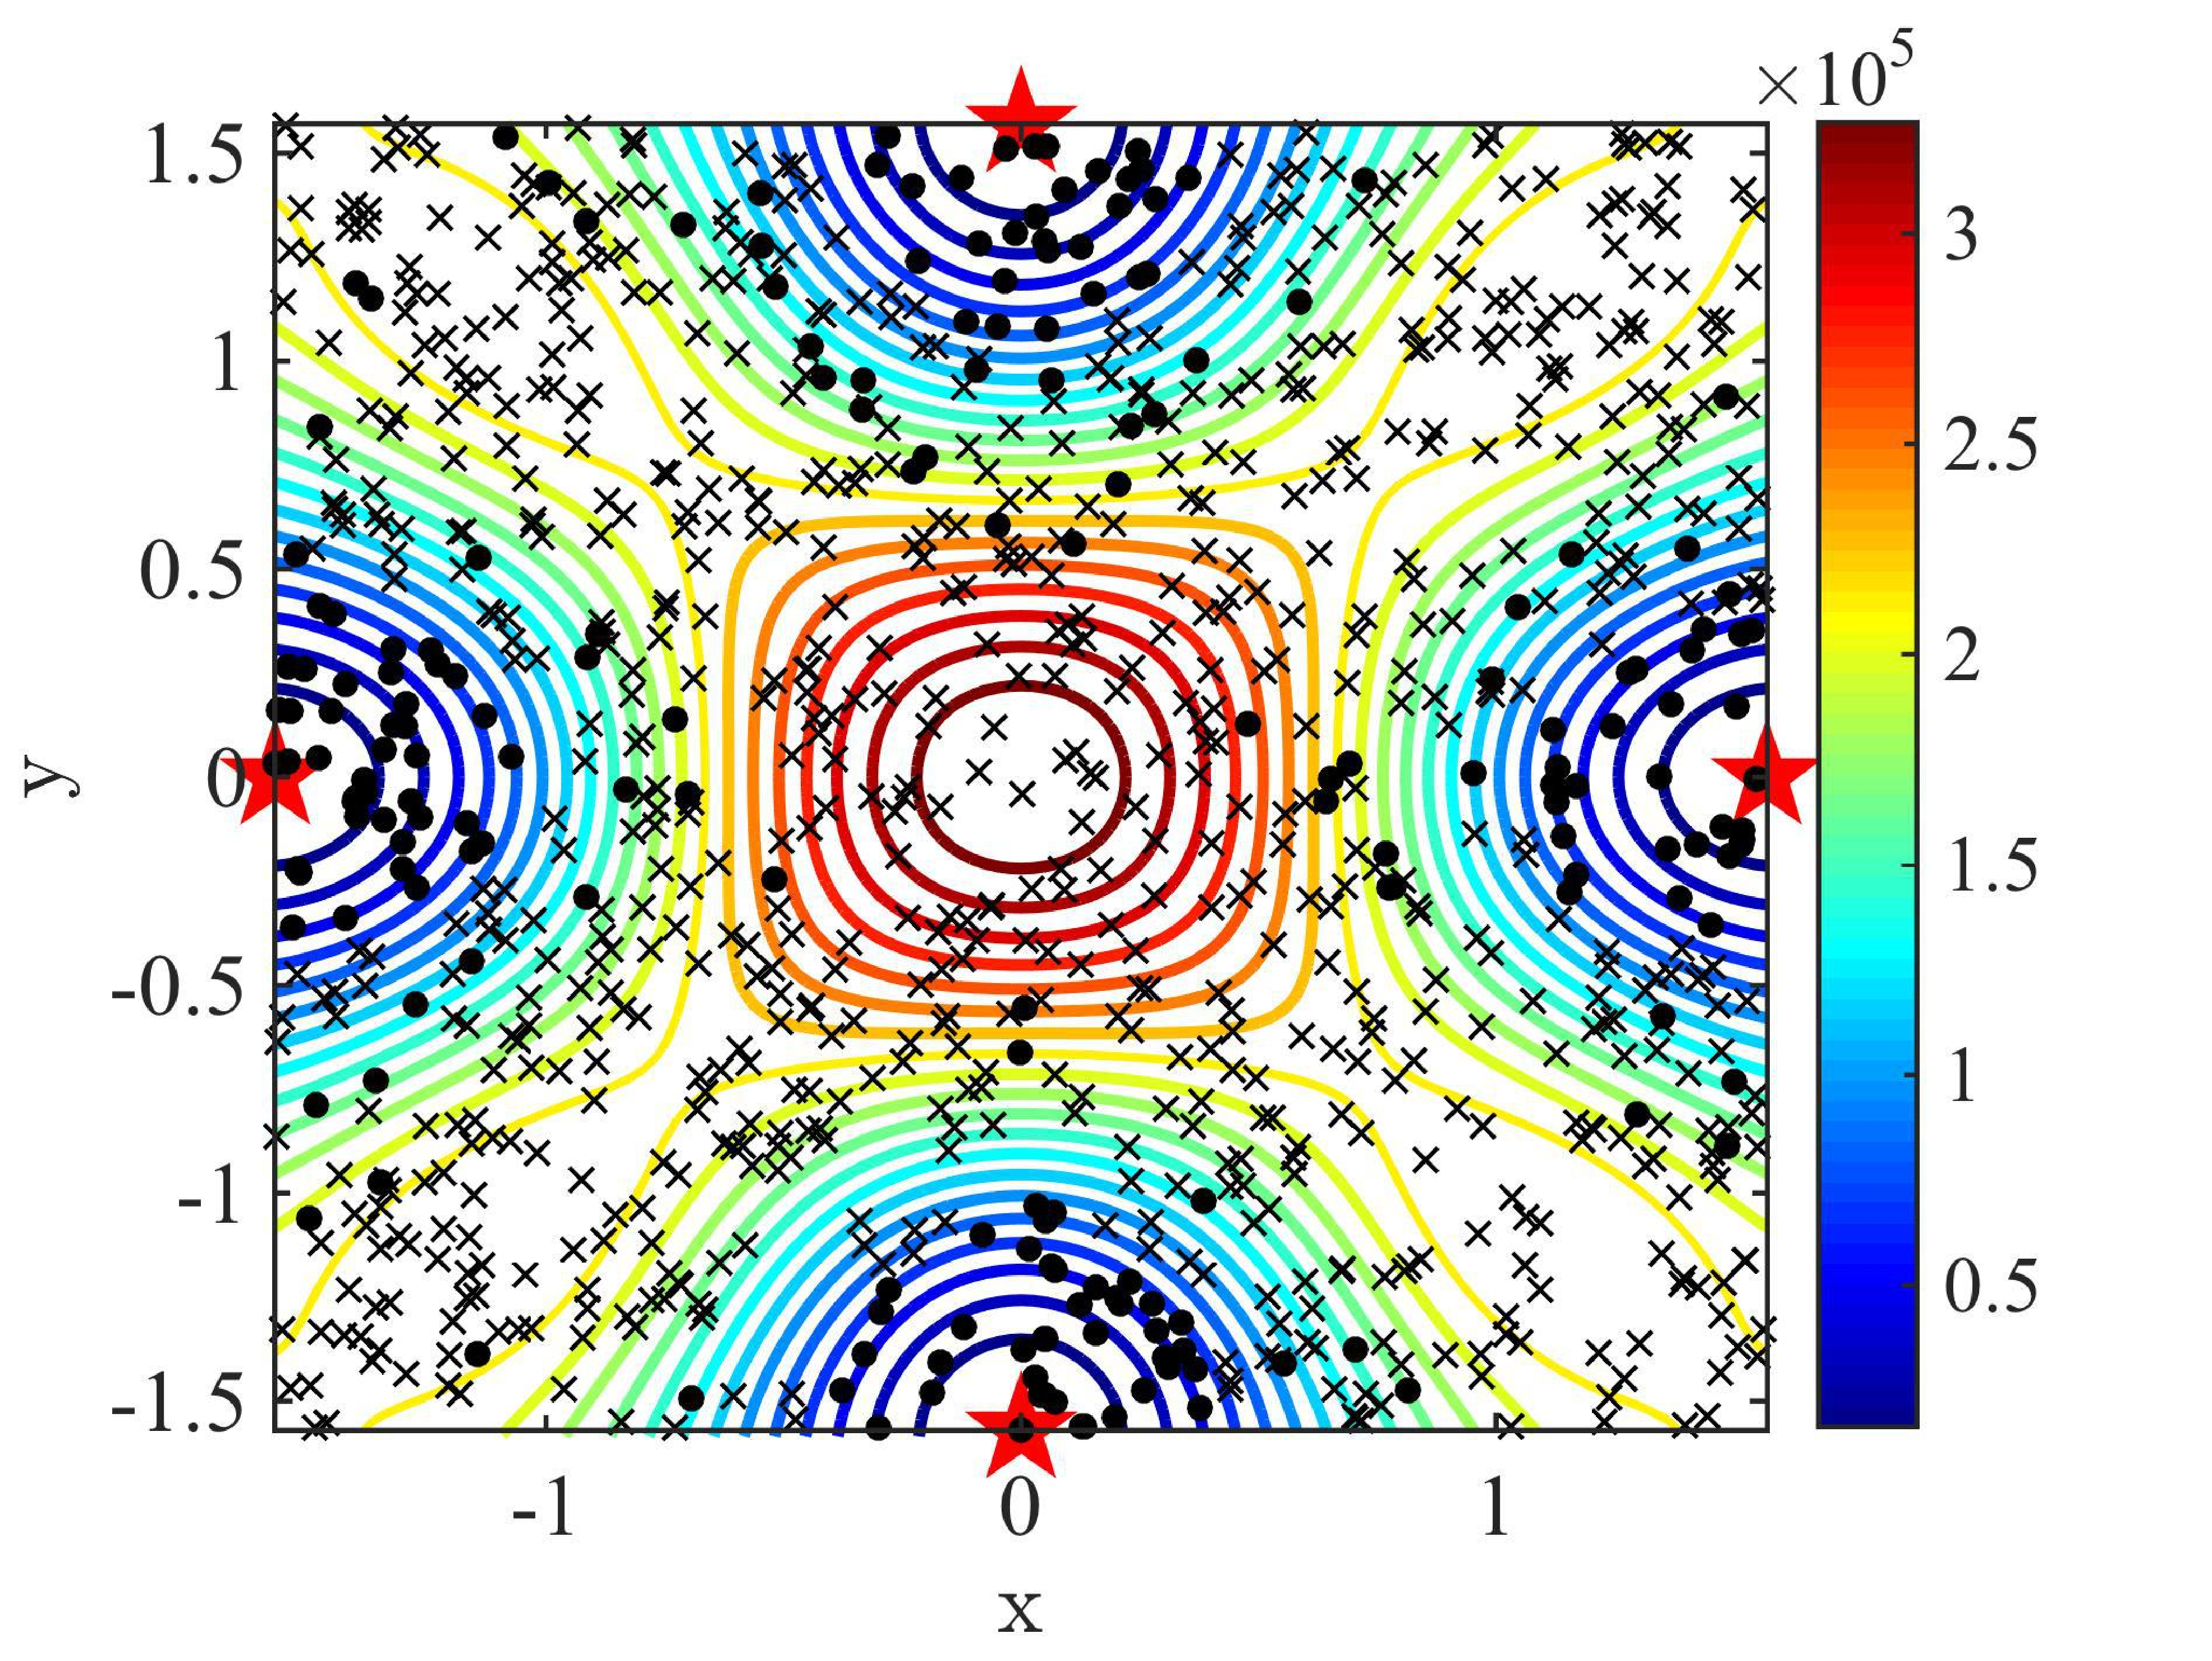
\includegraphics[width=0.47\textwidth]
   {figs/iso_shear_tangent_random.pdf}
 }
   \caption{Isotropic small deformation model: results of the Newton
     iterative scheme with a single random initial guess plotted on
     contours of the determinant function at bifurcation. A solid
     circle ($\bullet$) indicates that the initial point leads to a
     successful detection of bifurcation and its directions. A cross
     ($\times$) indicates failure. A total of 1000 random trials are
     performed for each parametrization.}
   \label{fig:iso-shear-robust}
\end{figure}

\subsection{Finite Deformation Anisotropic Hyperelastic Damage Model}
\label{subsec:anisotropic}

The second material model tested is a finite deformation anisotropic
hyperelastic damage model. Our aim is to study the effect of adding
complexity to the material model, and hence the tangent moduli, on the
performance of the different parametrizations. As in the previous
example, we first present the key features of the material model.

\subsubsection{Model Formulation}

The free energy function of the finite deformation anisotropic
hyperelastic damage model consists of an isotropic term and
direction-dependent terms. The motivation for this type of energy
formulation is to capture the behavior of materials with an isotropic
matrix and embedded microfibers with preferred directions, such as the
model proposed by \citet{Chen.etal:2014} to describe the behavior of
cladding for nuclear reactors subjected to damage by hydride
compounds. We assume that the damage affects both the matrix and the
microfibers. The free energy function is assumed to have the form
\begin{equation}\label{eq:aniso-energy}
  A(~C, ~M, \xi^\mtrx, \xi^\fiber_i)
  :=
  (1-\xi^\mtrx) f^\mtrx \Psi^\mtrx(~C)
  + \sum_{i=1}^{N} (1-\xi^\fiber_i) f^\fiber_i \Psi^\fiber_i(~C, ~M)
\end{equation}
where $~C$ is the right Cauchy-Green tensor, $~M$ is a unit vector
characterizing the preferred fiber direction, $f^\mtrx$ and
$f^\fiber_i$ are the volume fraction of the matrix and $i$th fiber,
$N$ is the number of fiber terms and $\xi^\mtrx$ and $\xi^\fiber_i$
are the damage factors corresponding to the matrix and the $i$th
fibers, respectively. In the following examples, we assume that there
are two preferred fiber directions.

We adopt a compressible Neo-Hookean type energy function for the
effective (undamaged) matrix component
\begin{equation}\label{eq:aniso-Psim0}
  \Psi^\mtrx (~C)
    = \frac{1}{8}\lambda (\log I_3)^2
    - \frac{1}{2}\mu \log I_3
    + \frac{1}{2}\mu( I_1 - 3)
\end{equation}
where $\lambda$ and $\mu$ play the role of the Lam\'{e} constants of
linear elasticity. For the microfibers we adopt the particular form of
strain-energy function proposed in \cite{Holzapfel.etal:2010}
\begin{equation}
  \Psi^\fiber_i(~C, ~M)
    = \frac{k_i}{q_i}
    \{ \exp[q_i(I_4 - 1)^2] \}
\end{equation}
where $k_i$ and $q_i$ are elastic constants for the $i$th fiber.  The
strain invariants $I_1$, $I_3$ and $I_4$ are defined as
\begin{gather}
  I_1 = \tr ~C,
  \quad
  I_3 = \det ~C,
  \quad
  I_4 = ~M \cdot (~C \cdot ~M).
\end{gather}
For the damage parameters, the same evolution law as in
\eref{eq:iso-xi} is used, except that for each phase of the material,
there is a different set of parameters as discussed in
\citet{Chen.etal:2014}.

Given the energy function \eref{eq:aniso-energy}, the fourth-order
tangent moduli tensor can be derived as
\begin{equation}\label{eq:aniso-tangent}
  \bbC
  : =
  (1-\xi^\mtrx) \bbC^\mtrx
  +
  \sum_{i=1}^N (1-\xi^\fiber_i) \bbC^\fiber_i
  -
  \beta^\mtrx {\xi^\mtrx}'  (~S^\mtrx \otimes ~S^\mtrx )
  -
  \sum_i^n \beta^\fiber_i {\xi^\fiber_i}' (~S^\fiber_i \otimes ~S^\fiber_i)
\end{equation}
where $\beta^\mtrx = 1$ if the damage of the matrix evolves within the
time increment or $\beta^\mtrx=0$ otherwise; $\beta^\fiber_i = 1$ if
the damage of the $i$th fiber evolves within the time increment or
$\beta^\fiber_i=0$ otherwise; ${\xi^\mtrx}'$ and ${\xi^\fiber_i}'$ are
the derivatives of the damage parameters defined in \eref{eq:iso-xi}
with respect to the maximum thermodynamic force defined in
\eref{eq:alpha}; and $~S^\mtrx$ and $~S^\fiber_i$ are the effective
(undamaged) second Piola-Kirchhoff stresses for the matrix and the
$i$th fibers given by
\begin{equation}\label{eq:aniso-S0m}
  ~S^\mtrx
  :=
  2 f^\mtrx \frac{\partial \Psi^\mtrx}{\partial~C}
\end{equation}
and
\begin{equation}\label{eq:aniso-S0i}
  ~S^\fiber_i
  :=
  2 f^\fiber_i \frac{\partial \Psi^\fiber_i}{\partial~C}
\end{equation}
where $f^\mtrx$ and $f^\fiber_i$ are the volume fraction of the matrix
and $i$th fiber, respectively.

The effective tangent moduli tensors can be calculated as
\begin{equation}\label{eq:aniso-tangent1}
  \bbC^\mtrx
  :=
  2 \frac{\partial ~S^\mtrx}{\partial~C}
\end{equation}
and
\begin{equation}\label{eq:aniso-tangent2}
  \bbC^\fiber_i
  :=
  2 \frac{\partial ~S^\mtrx}{\partial~C}.
\end{equation}

It should be noted that the fourth-order tangent $\bbC$ from
\eref{eq:aniso-tangent} is computed as the second derivative of the
strain energy with respect to the right Cauchy-Green deformation
tensor $~C$. The strong ellipticity condition
\eref{eq:strong-ellipticity} requires the tangent $\bbA$ that is
obtained as the second derivative of the strain energy with respect to
the deformation gradient $~F$. One tangent can be converted to the
other using the following relation (in indicial notation)
\begin{equation}\label{eq:aniso-tangent3}
  \bbA_{ijkl} = S_{lj} \delta_{ik}
    + F_{ip} \bbC_{pjlq} F_{kq}
\end{equation}
where $S_{lj}$ are the components of the second Piola-Kirchhoff stress
(including damage contribution) of the corresponding phase (e.g.,
matrix or fiber component), $\delta_{ik}$ is the Kronecker delta and
$F_{ij}$ are the components of the deformation gradient.

\subsubsection{Uniaxial Tension Test}

The finite deformation anisotropic model is tested under monotonically
increasing uniaxial tension loading illustrated in Figure~\ref{fig:composite_tension}.
\begin{figure}[!htbp]
 \centering
      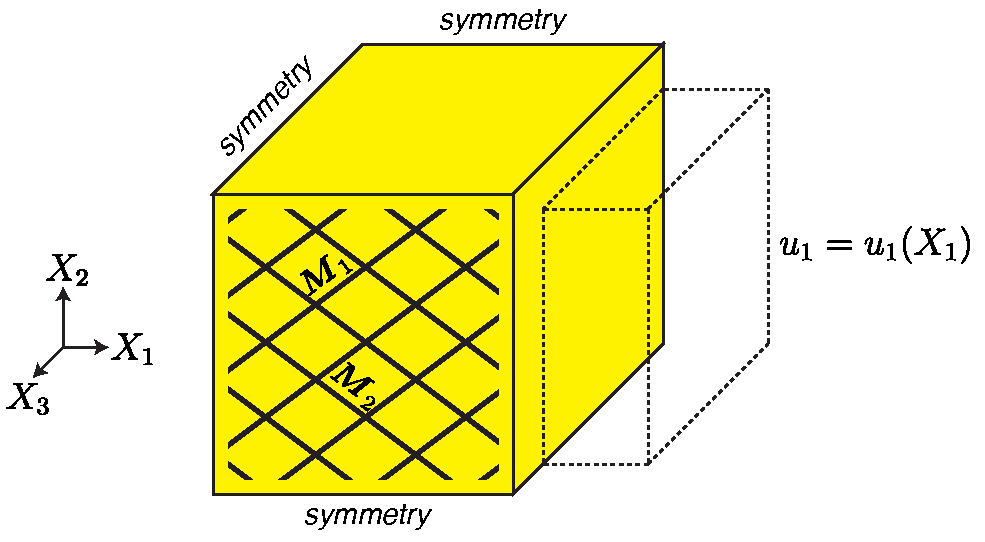
\includegraphics[width=120mm]{figs/composite_tension_schematic.pdf}
     \caption{Schematic illustrating the uniaxial tension of a reinforced-fiber composite under finite deformations. Fibers are oriented along $\bM_{1}$ and $\bM_{2}$.}
     \label{fig:composite_tension}
\end{figure}
The material properties for both
the matrix and microfibers are listed in Table~
\ref{tab:aniso-material}.

\begin{table}[htbp]
  \begin{center}
    \begin{tabular}{ l l l l }
      \toprule
      Matrix
      &

      &

      Fibers

      &
      \\
      \midrule
      Lam\'{e} constant
      &
      $\lambda=80$
      &
      Elasticity constants
      &
      $k_1 = k_2 = 100$
      \\
      Lam\'{e} constant
      &
      $\mu = 80$
      &
      Elasticity constants
      &
      $q_1 = q_2 = 1.0$
      \\
      Damage variable
      &
      $\xi^\mtrx_\infty = 1.0$
      &
      Damage variable
      &
      $\xi^\fiber_{\infty;1} = \xi^\fiber_{\infty;2} = 1.0$
      \\
      Damage variable
      &
      $\tau^\mtrx = 4.0$
      &
      Damage variable
      &
      $\tau^\fiber_1 = \tau^\fiber_2 = 4.0$
      \\
      Volume fraction
      &
      $f^\mtrx = 0.2$
      &
      Volume fraction
      &
      $f^\fiber_1 = f^\fiber_2 = 0.4$
      \\
      &

      &
      Direction vector
      &
      $~M_1 = \{ 0.8,~0.6,~0.0\}$
      \\
      &

      &

      &
      $~M_2 = \{ 0.8,-0.6,~0.0\}$
      \\
      \bottomrule
    \end{tabular}
    \caption{Material properties for anisotropic damage model}
    \label{tab:aniso-material}
  \end{center}
\end{table}

The axial stress \vs stretch behavior of the uniaxial tension test is
shown in \fref{fig:aniso-stress_stretch}(a), where the X denotes the
onset of material bifurcation. We use the two-step procedure together
with the adaptive time increment discussed in \sref{sec:detection} for
the detection of bifurcation. \fref{fig:aniso-stress_stretch}(b) shows
the degradation of the determinant function for all five
parametrizations until material bifurcation is detected. In this
loading test, all five parametrizations detect bifurcation at the same
time, \ie, when the axial component of the deformation gradient
$F_{11} = 1.1798$.

\begin{figure}[!htbp]
  \centering \subfigure[]{
    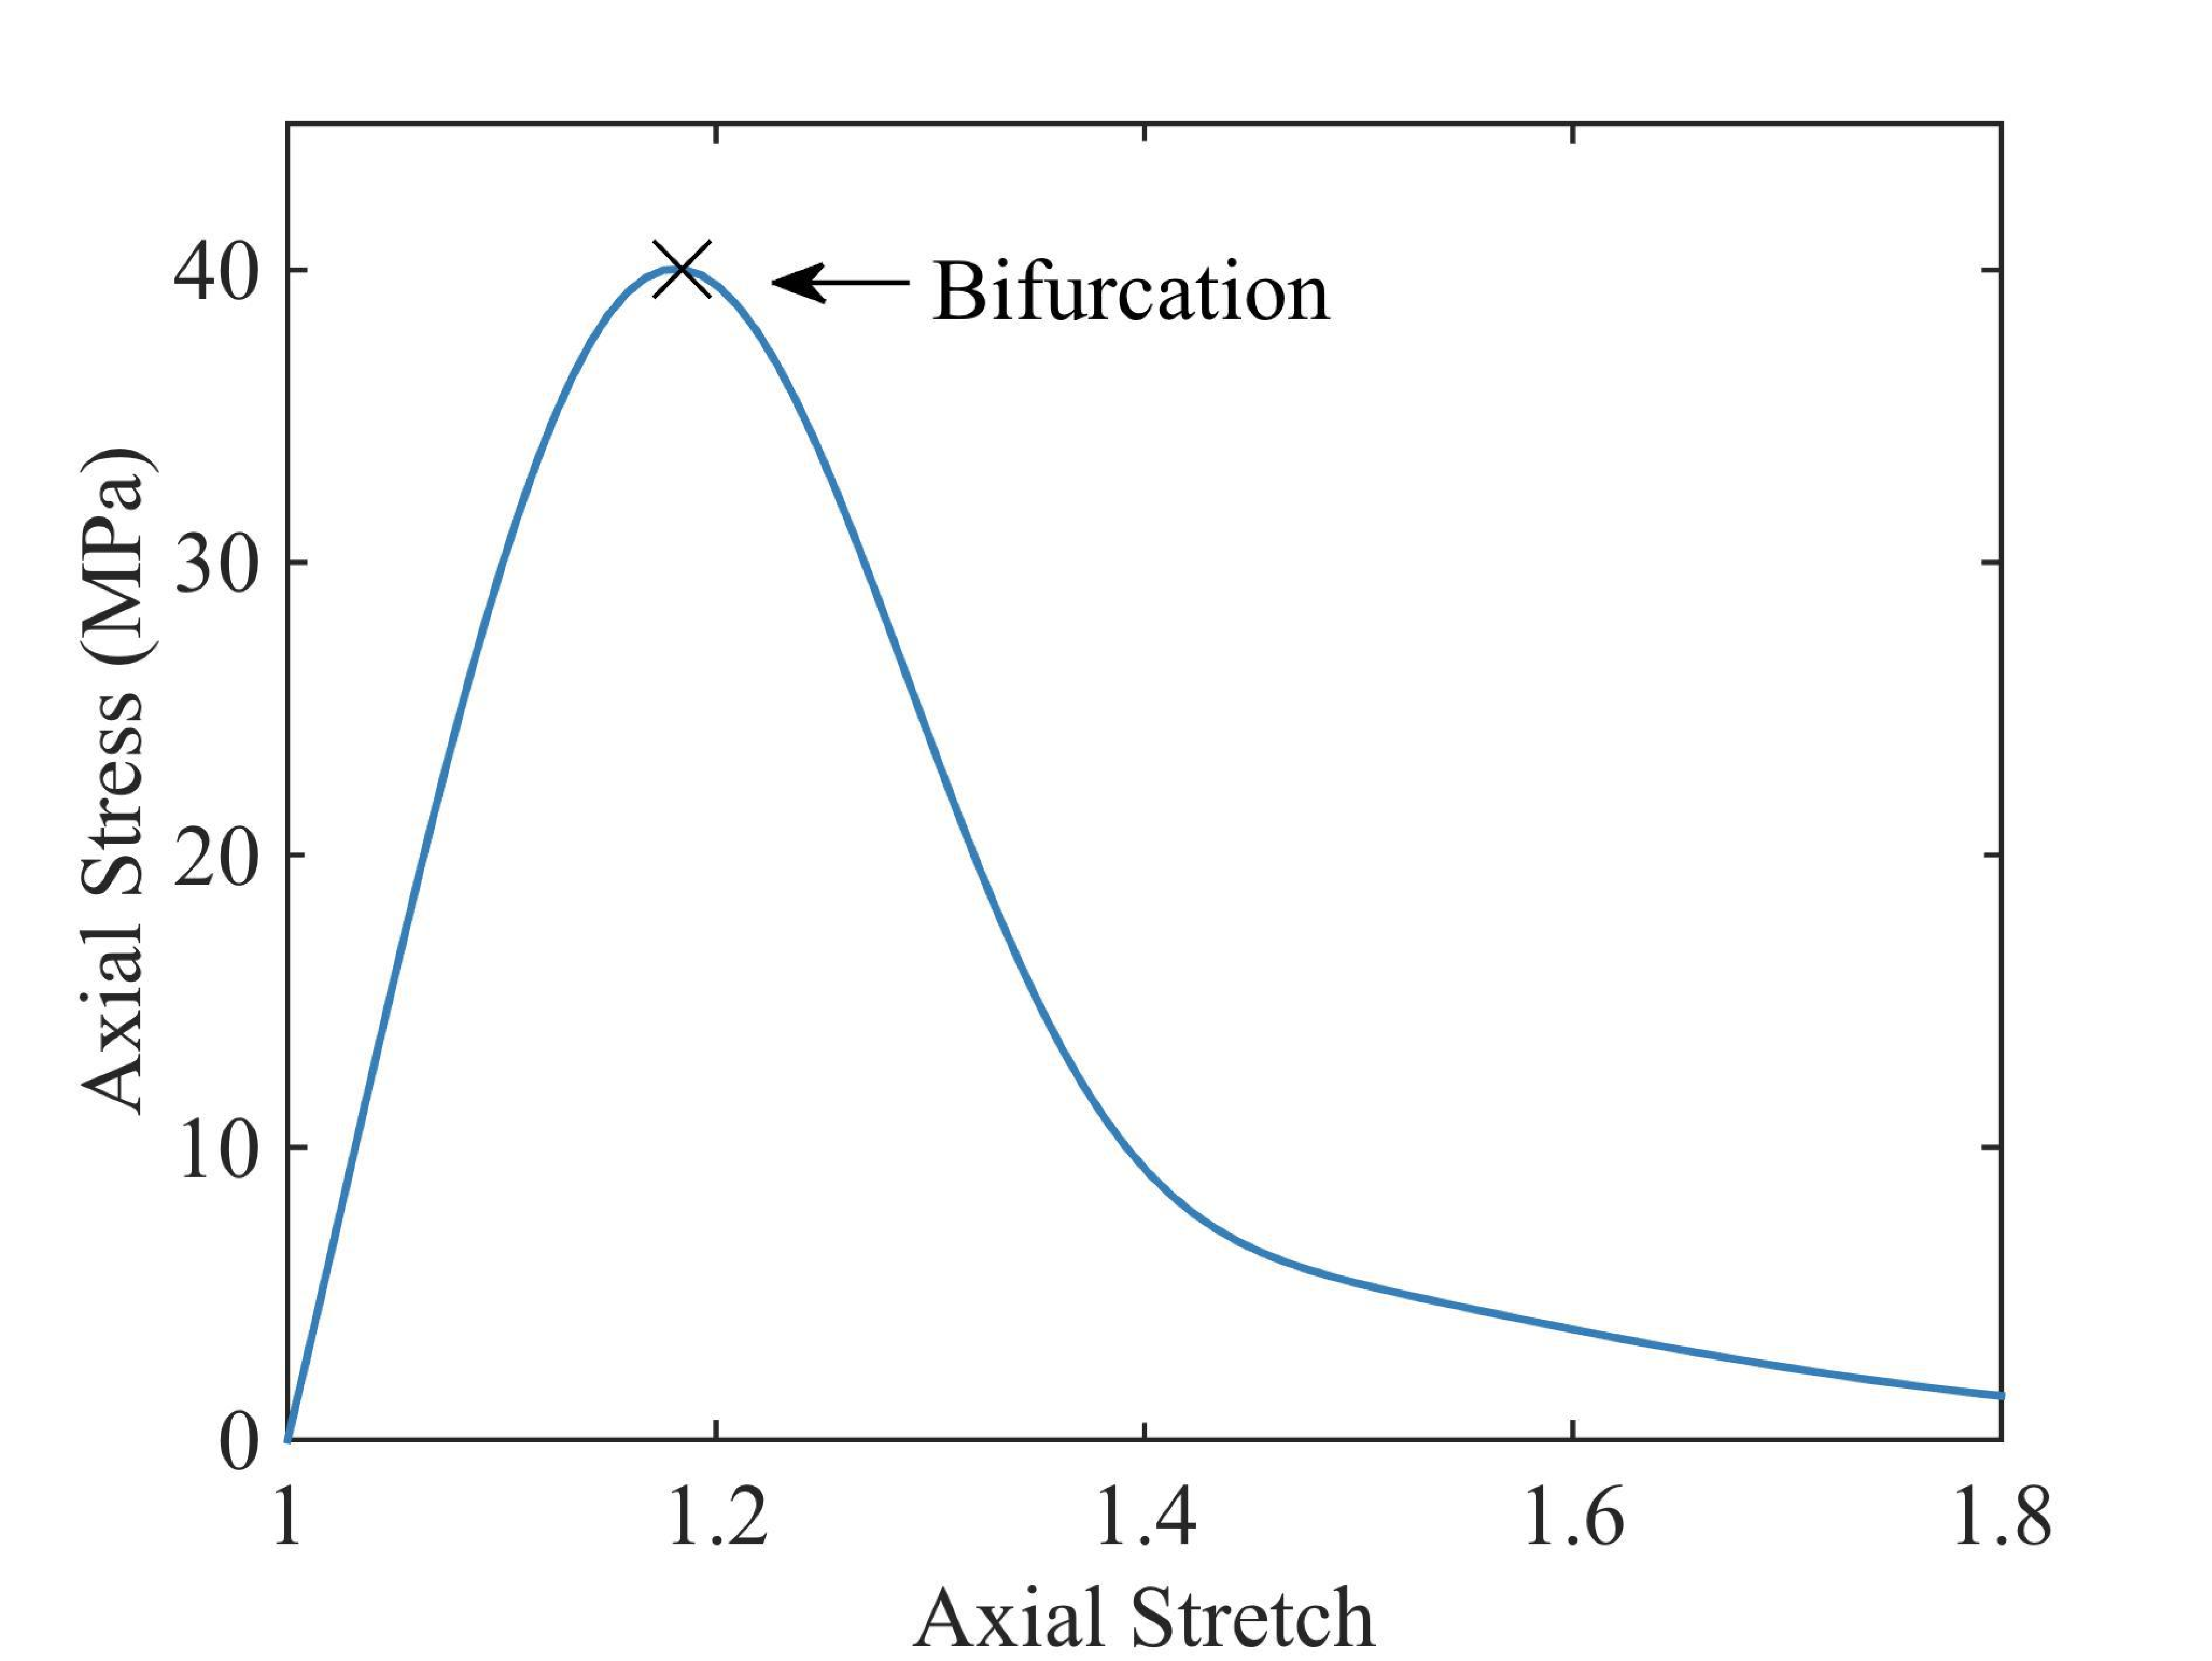
\includegraphics[width=0.60\textwidth]
    {figs/aniso_uniaxial_stress_stretch.pdf}
  } \subfigure[]{
    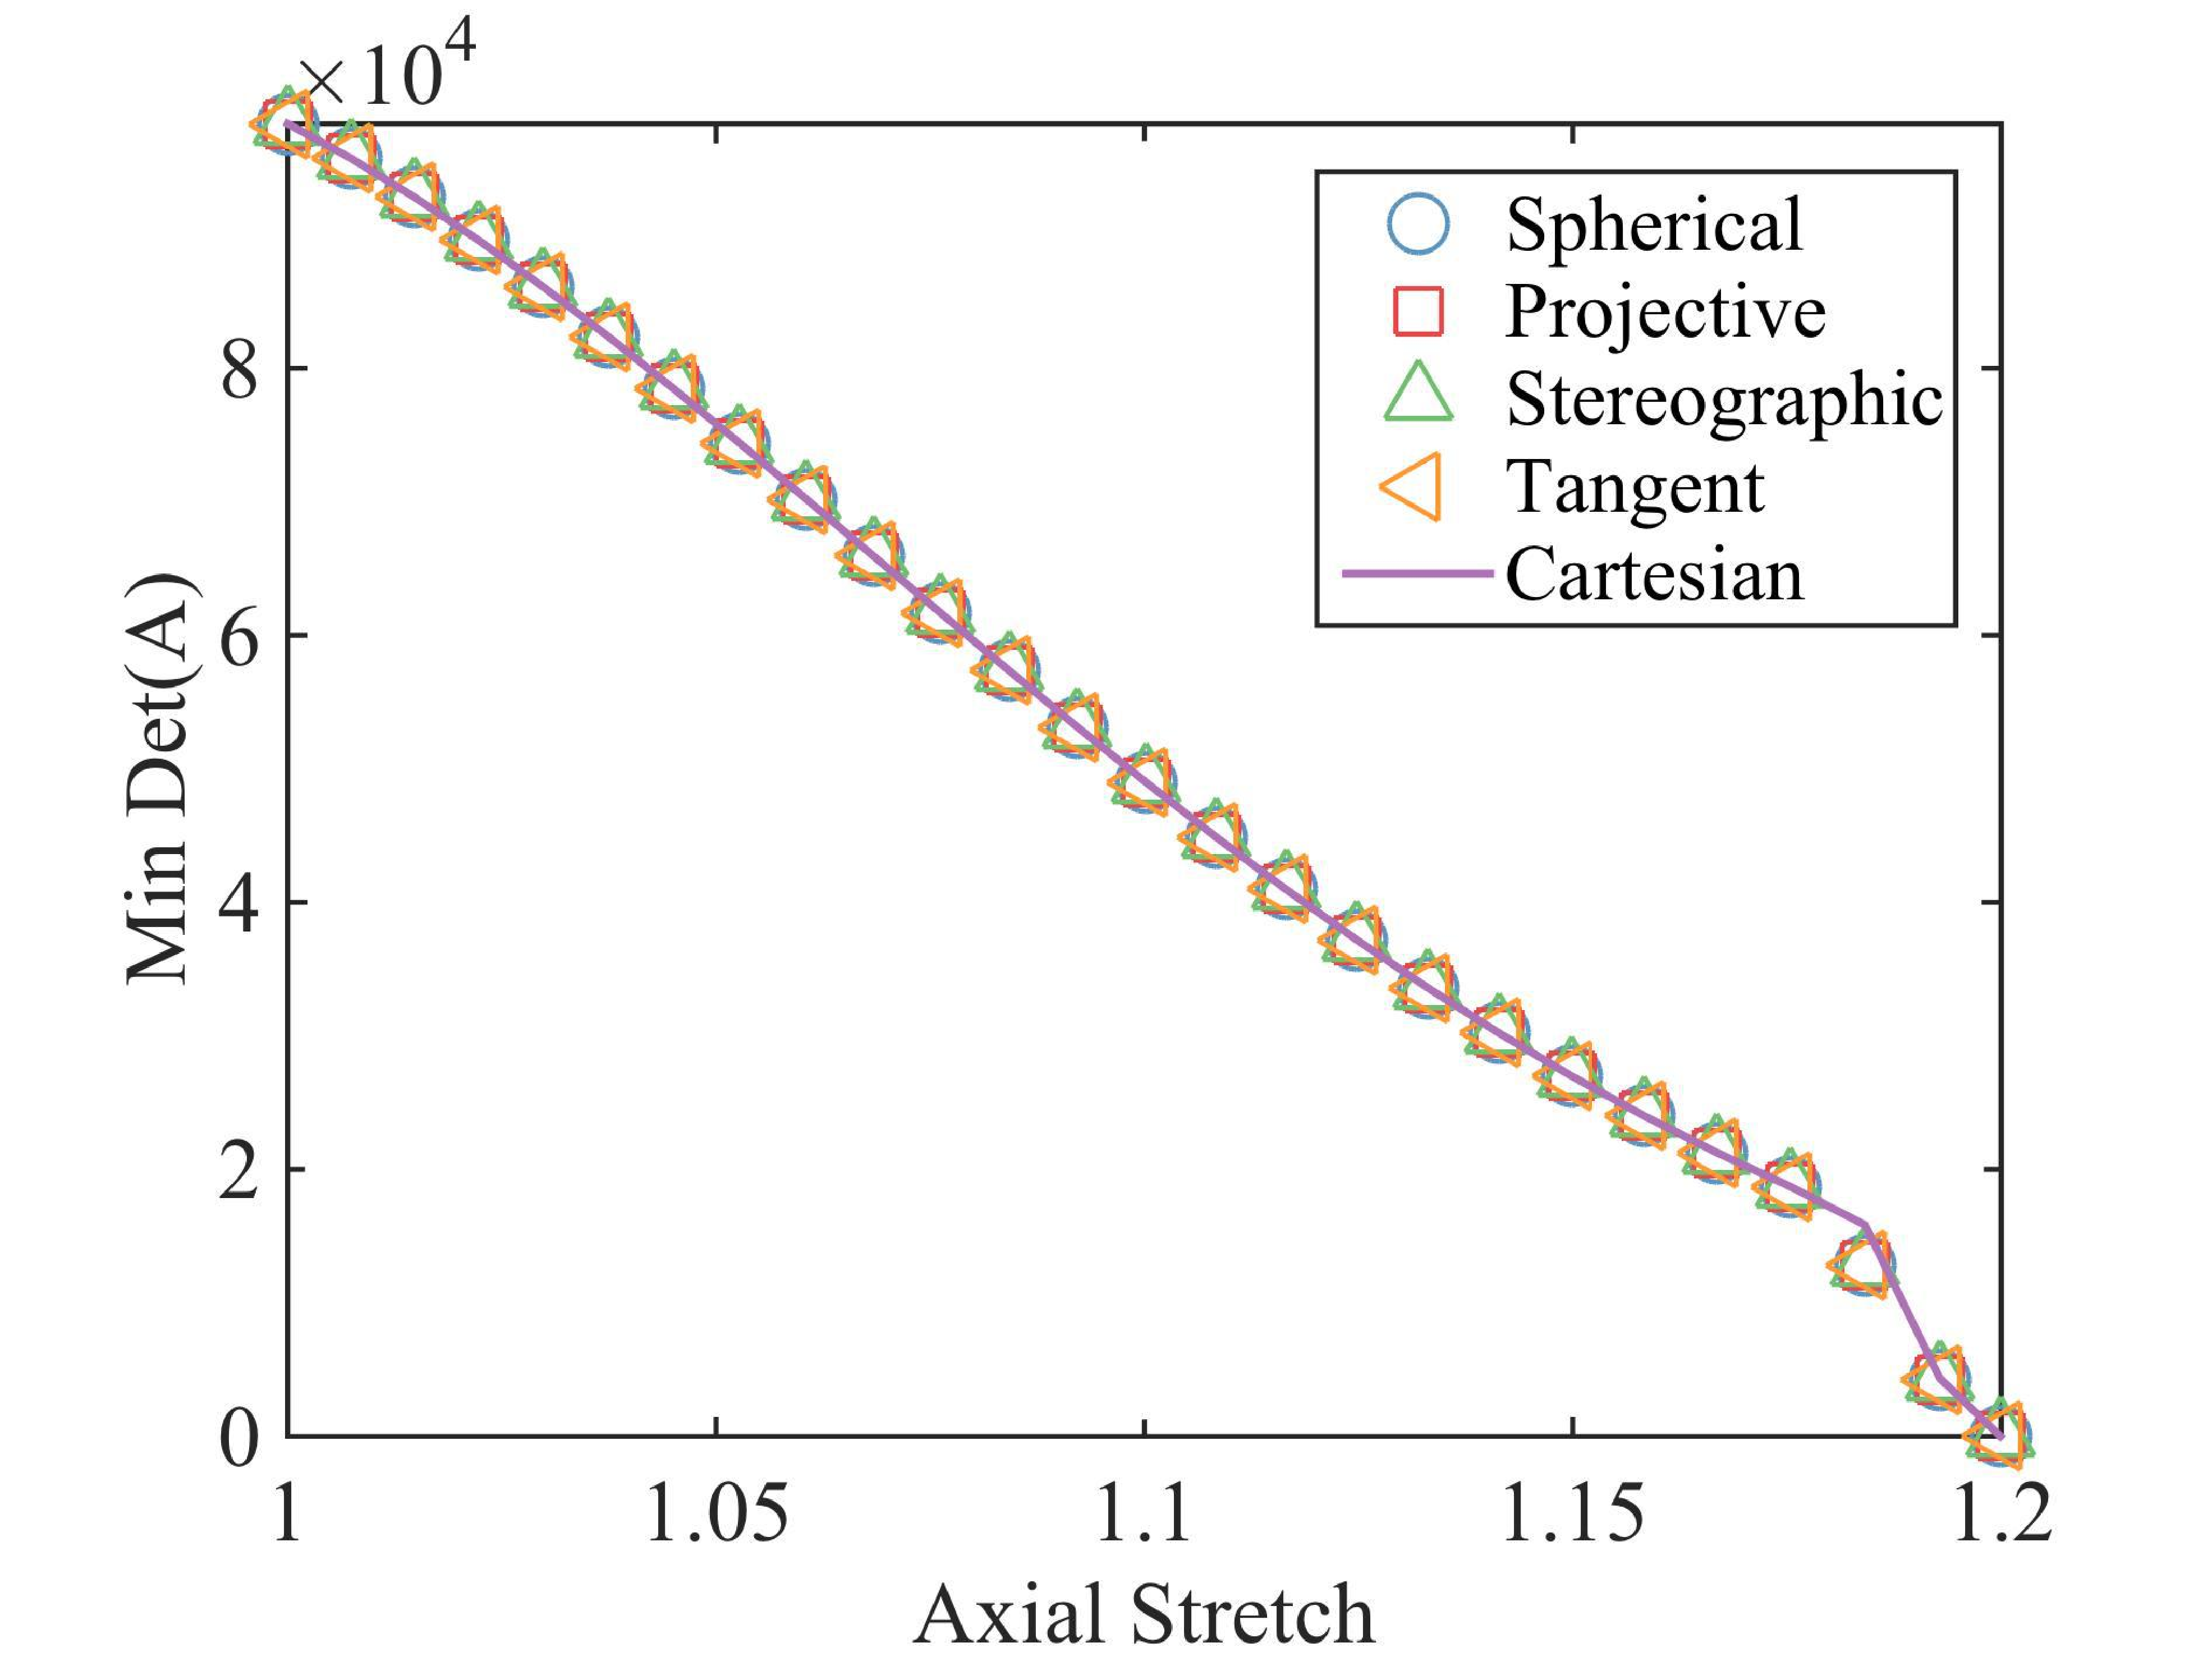
\includegraphics[width=0.60\textwidth]
    {figs/aniso_uniaxial_mindetA_stretch.pdf}
  }
  \caption{Uniaxial tension test on finite deformation anisotropic
    damage model: (a)stress vs. axial stretch, with the X indicating
    bifurcation, and (b) degradation of $\det~A$ for different
    parametrizations.}
  \label{fig:aniso-stress_stretch}
\end{figure}

As in the previous example, the computation time of the different
parametrizations within the loading increment leading to bifurcation
is recorded and shown in
Table~\ref{tab:aniso-uniaxial-runtime}. Again, the density of the
initial sampling is represented by the sampling interval and the
number of sampling points. In general, as the number of sampling
points decreases, so does the computation time.  Fewer sampling
points, however, may lead to a poor initial guess for the Newton
iterative scheme, which may result in a greater overall computation
time to arrive at a converged solution. Due to the added complexity of
the material model, different parametrizations are more sensitive to
the density of the initial sampling grids. The spherical
parametrization fails to correctly detect the bifurcation when the
sampling interval is greater than 0.6. The stereographic, projective
and tangent parametrizations, though more robust in this case, are
computationally more expensive.  The Cartesian parametrization is
computationally efficient and at the same time, relatively insensitive
to the sampling interval.

\begin{table}[!htbp]
  \begin{center}
    \begin{tabular}{c c | r r r r r}
      \toprule
      \multicolumn{2}{c}{Sampling} & \multicolumn{5}{c}{Run Time ($\mu$s)} \\
      Interval  & Points  & Spherical & Stereographic & Projective &
      Tangent & Cartesian \\
      \midrule
      0.05  &  41  &  404  & 254  &  5828  &  330  &  412   \\
      0.1  &  21  &  224  & 207  &  926   &  212  &  214   \\
      0.2  &  11  &  192  & 181  &  296   &  187  &  122   \\
      0.3  &  7  &  174  & 210  &  250   &  187  &  132   \\
      0.4  &  5  &  217  & 208  &  268   &  189  &  111   \\
      0.5  &  5  &	176  & --  &  239   &  --   &  123   \\
      0.6  &  3  &	171  & 173  &  228   &  215  &  281   \\
      0.7  &  3  &	208  & 175 	  &  193   &  157  &  141   \\
      0.8  &  3  &  --  & 213  &  187   &  183  &  101   \\
      0.9  &  3  &	 --  & 214  &  225   &  204  &  99   \\
      1.0  &  3  &  --  & --	  &  225   &  --   &  118   \\
      1.5  &  1  &	 --  & --	  &  --   &  --   &  --   \\
      \bottomrule
    \end{tabular}
    \caption{Computation time for different parametrizations in the
      uniaxial tension test within the loading increment leading to
      bifurcation.  The dash ``--'' indicates that the parametrization
      fails to detect bifurcation in this loading increment.}
    \label{tab:aniso-uniaxial-runtime}
  \end{center}
\end{table}

To gain insights into the influence of the parametrizations on the
determinant function $\det~A$ as loading proceeds, we plot in
\fref{fig:aniso-spherical-detA} to \fref{fig:aniso-cartesian-detA} the
landscapes at four different axial stretch levels for different
parametrizations. Moreover, the corresponding plane views of the 
determinant landscapes at the bifurcation are also shown in
\fref{fig:aniso-uniaxial-detAXplane}, where the white stars indicate global
minima.

\begin{figure}[!htbp]
   \centering \subfigure[$F_{11}=1.0074$]{
   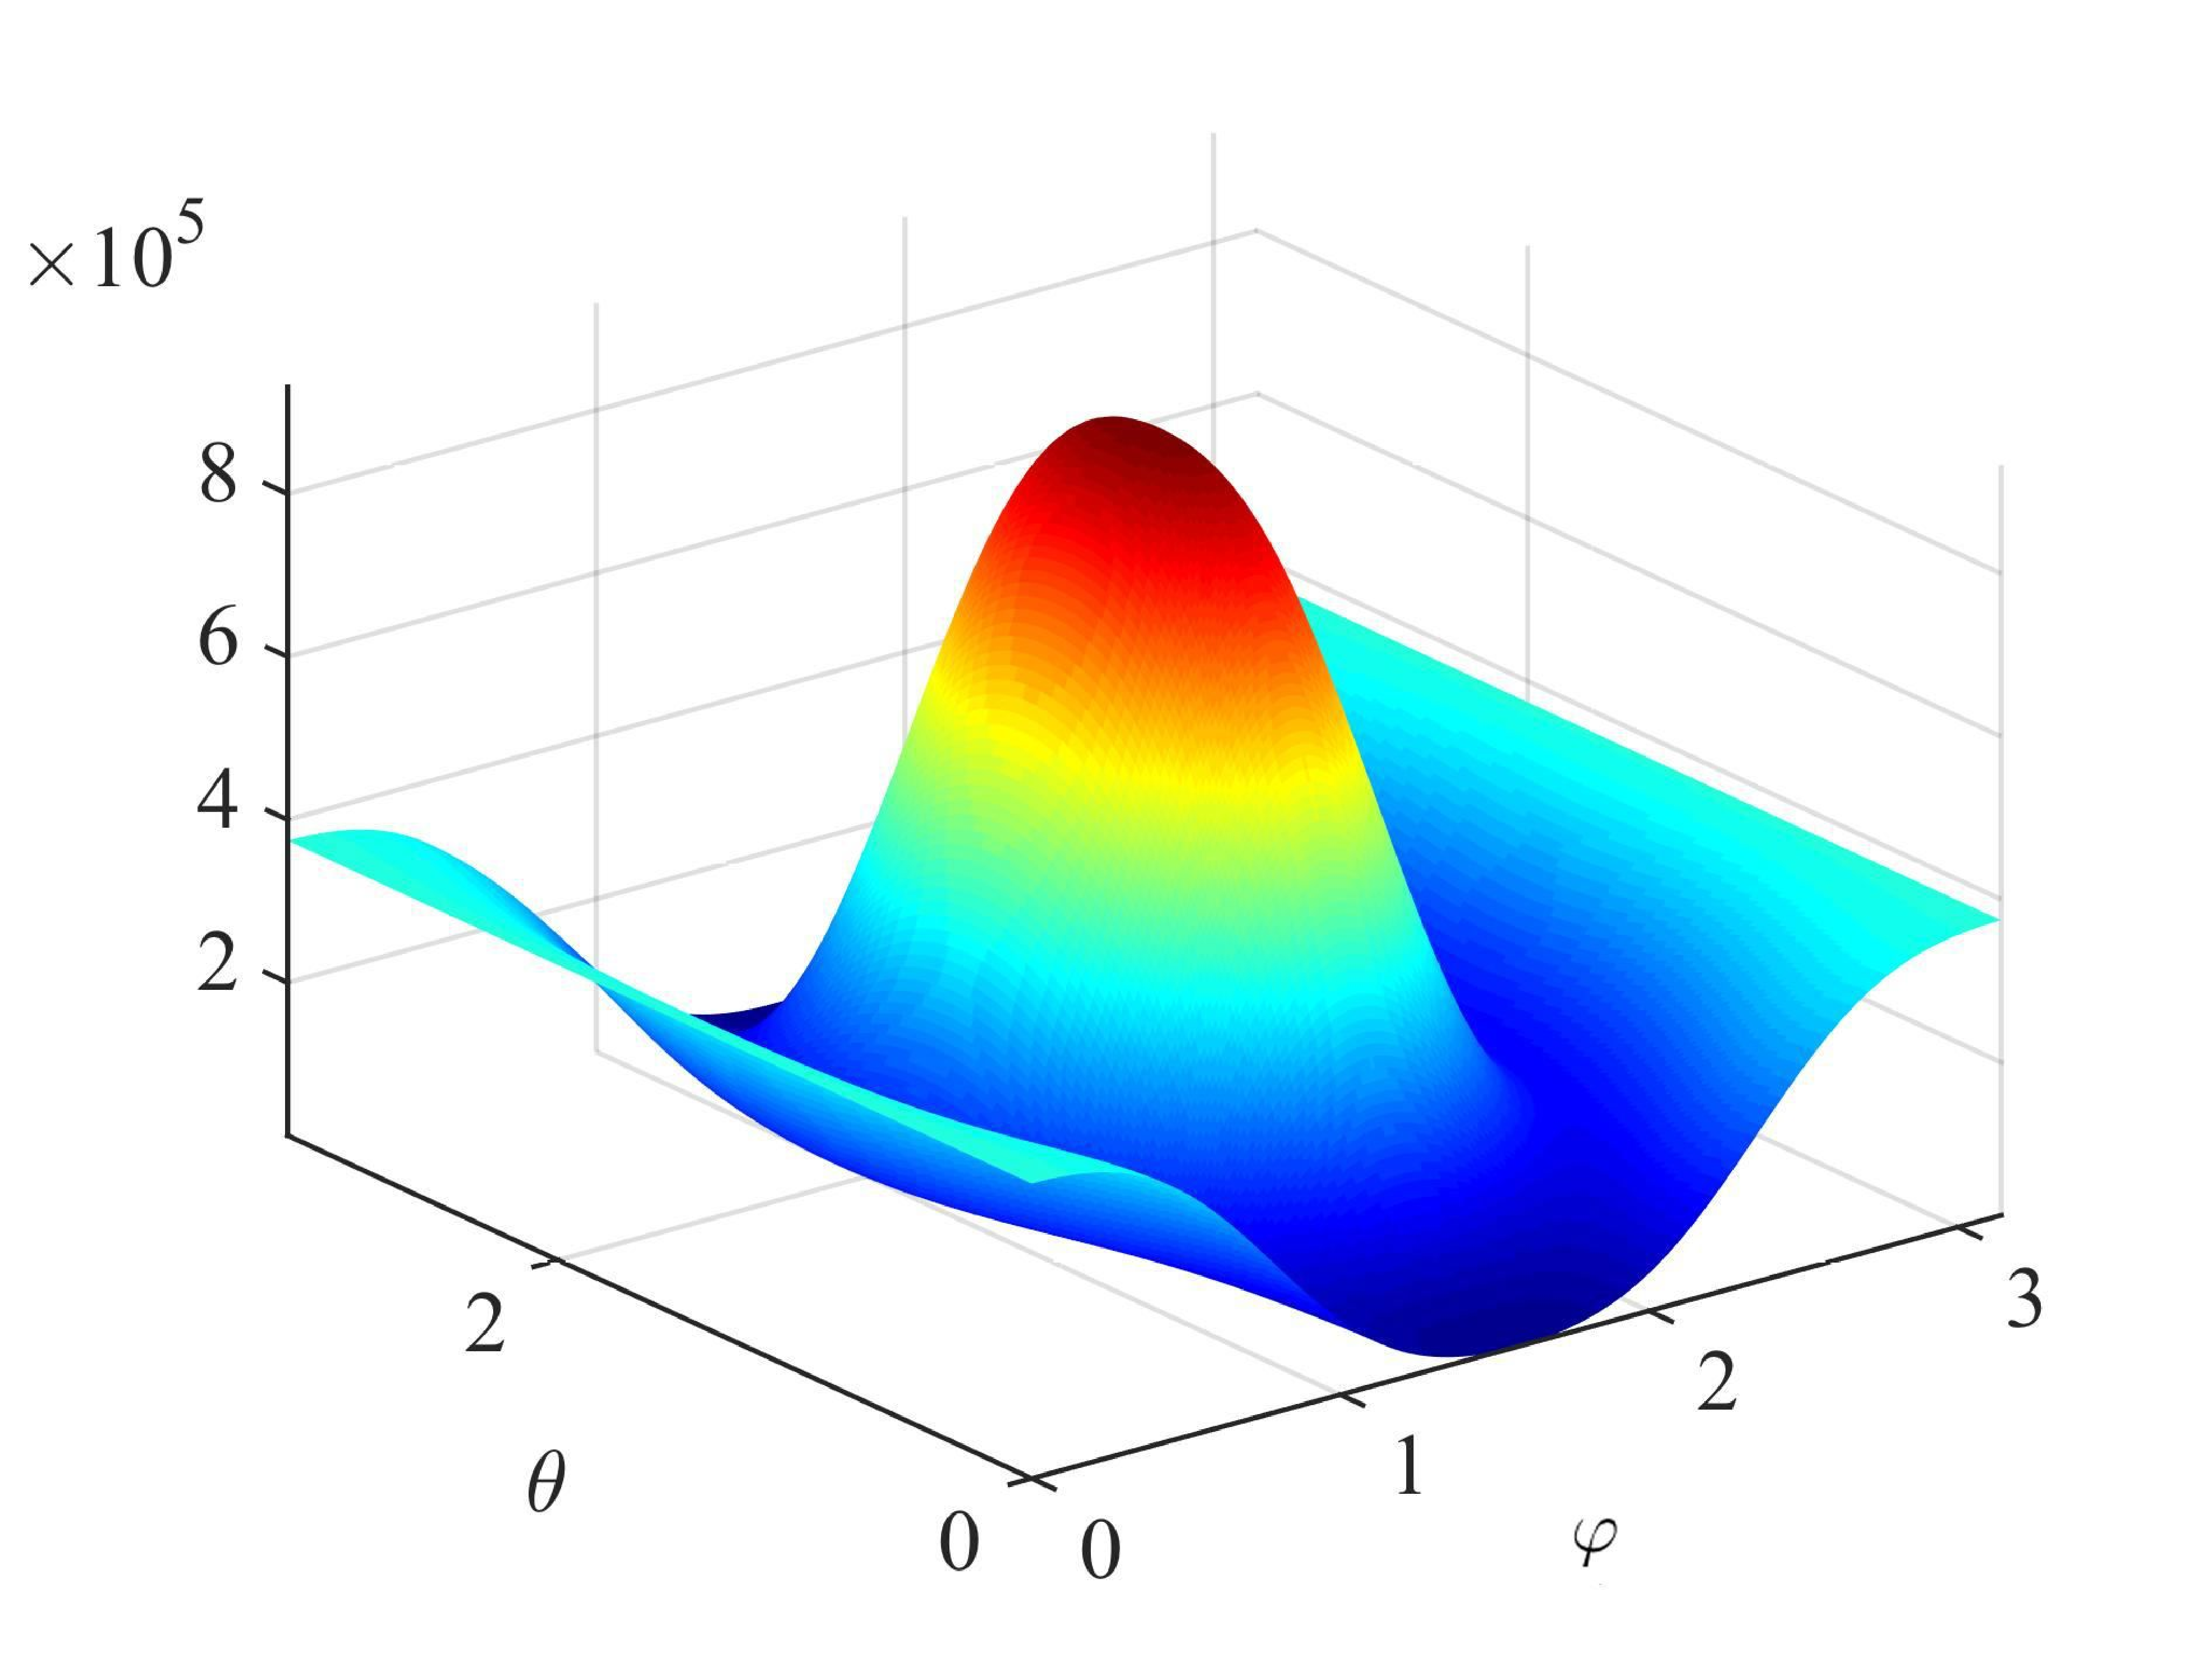
\includegraphics[width=0.45\textwidth]
   {figs/aniso_uniaxial_spherical_detA_F1p0074.pdf}
 } \subfigure[$F_{11}=1.0762$]{
   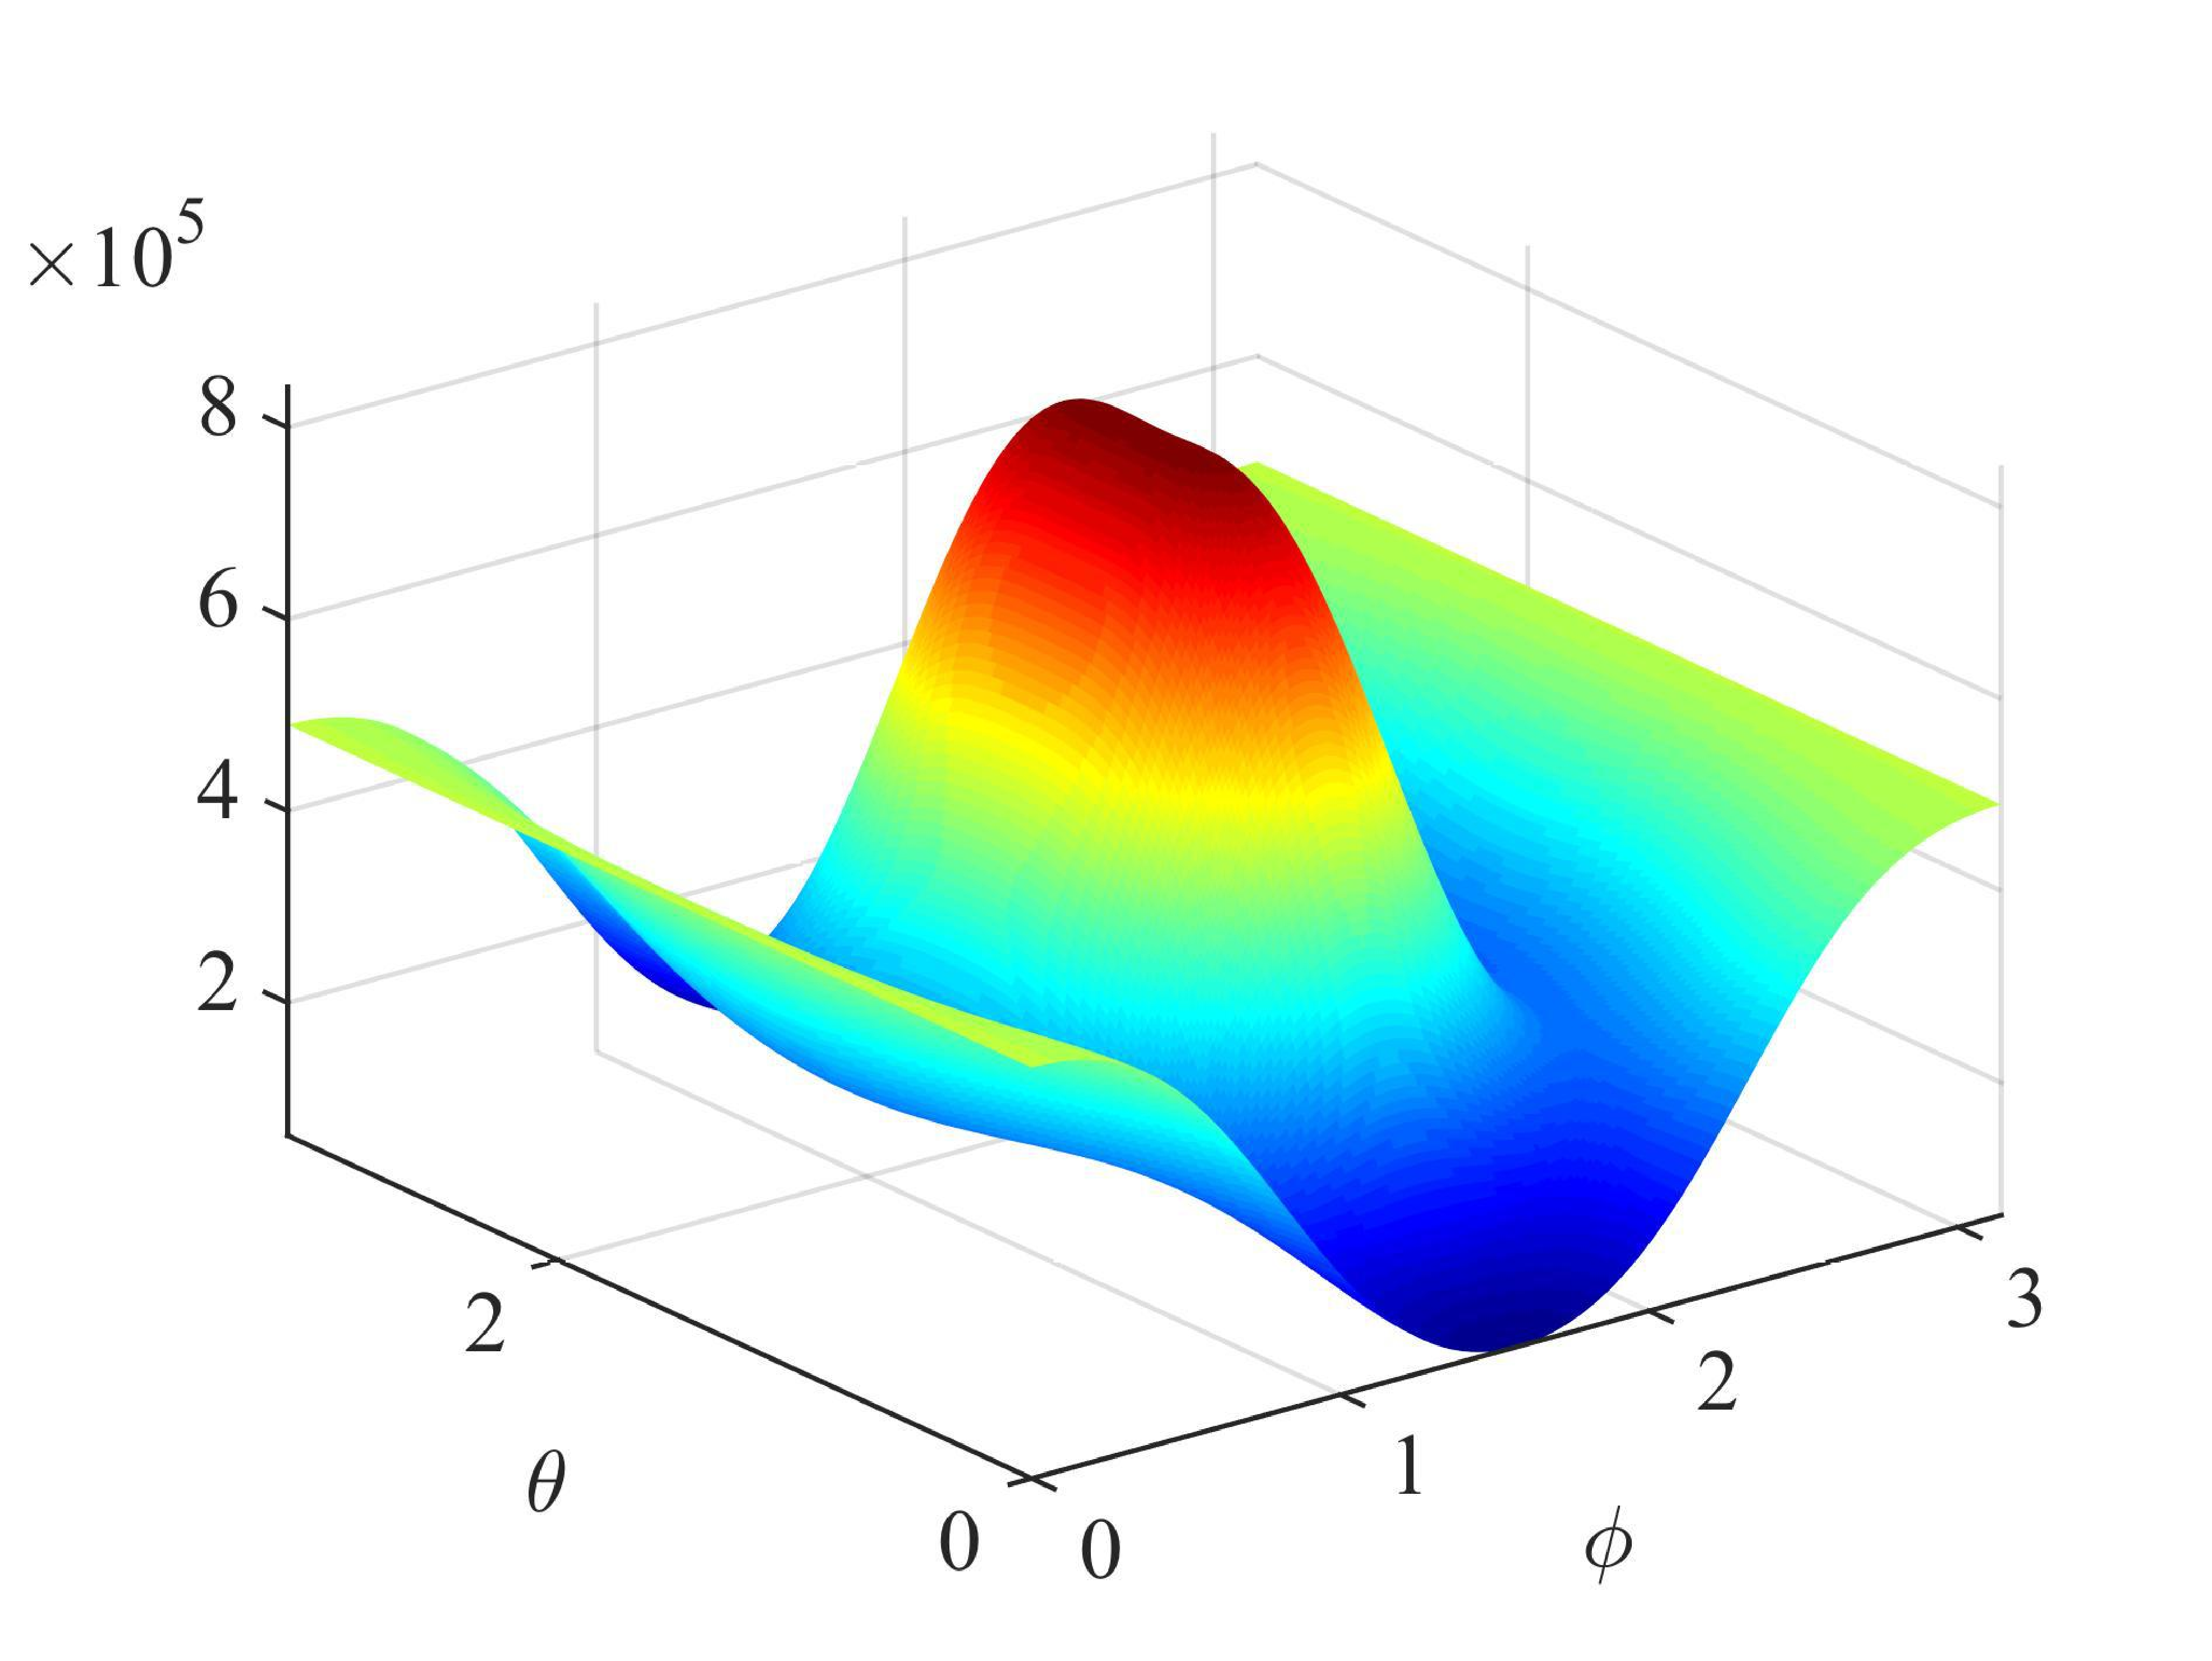
\includegraphics[width=0.45\textwidth]
   {figs/aniso_uniaxial_spherical_detA_F1p0762.pdf}
 } \subfigure[$F_{11}=1.1583$]{
   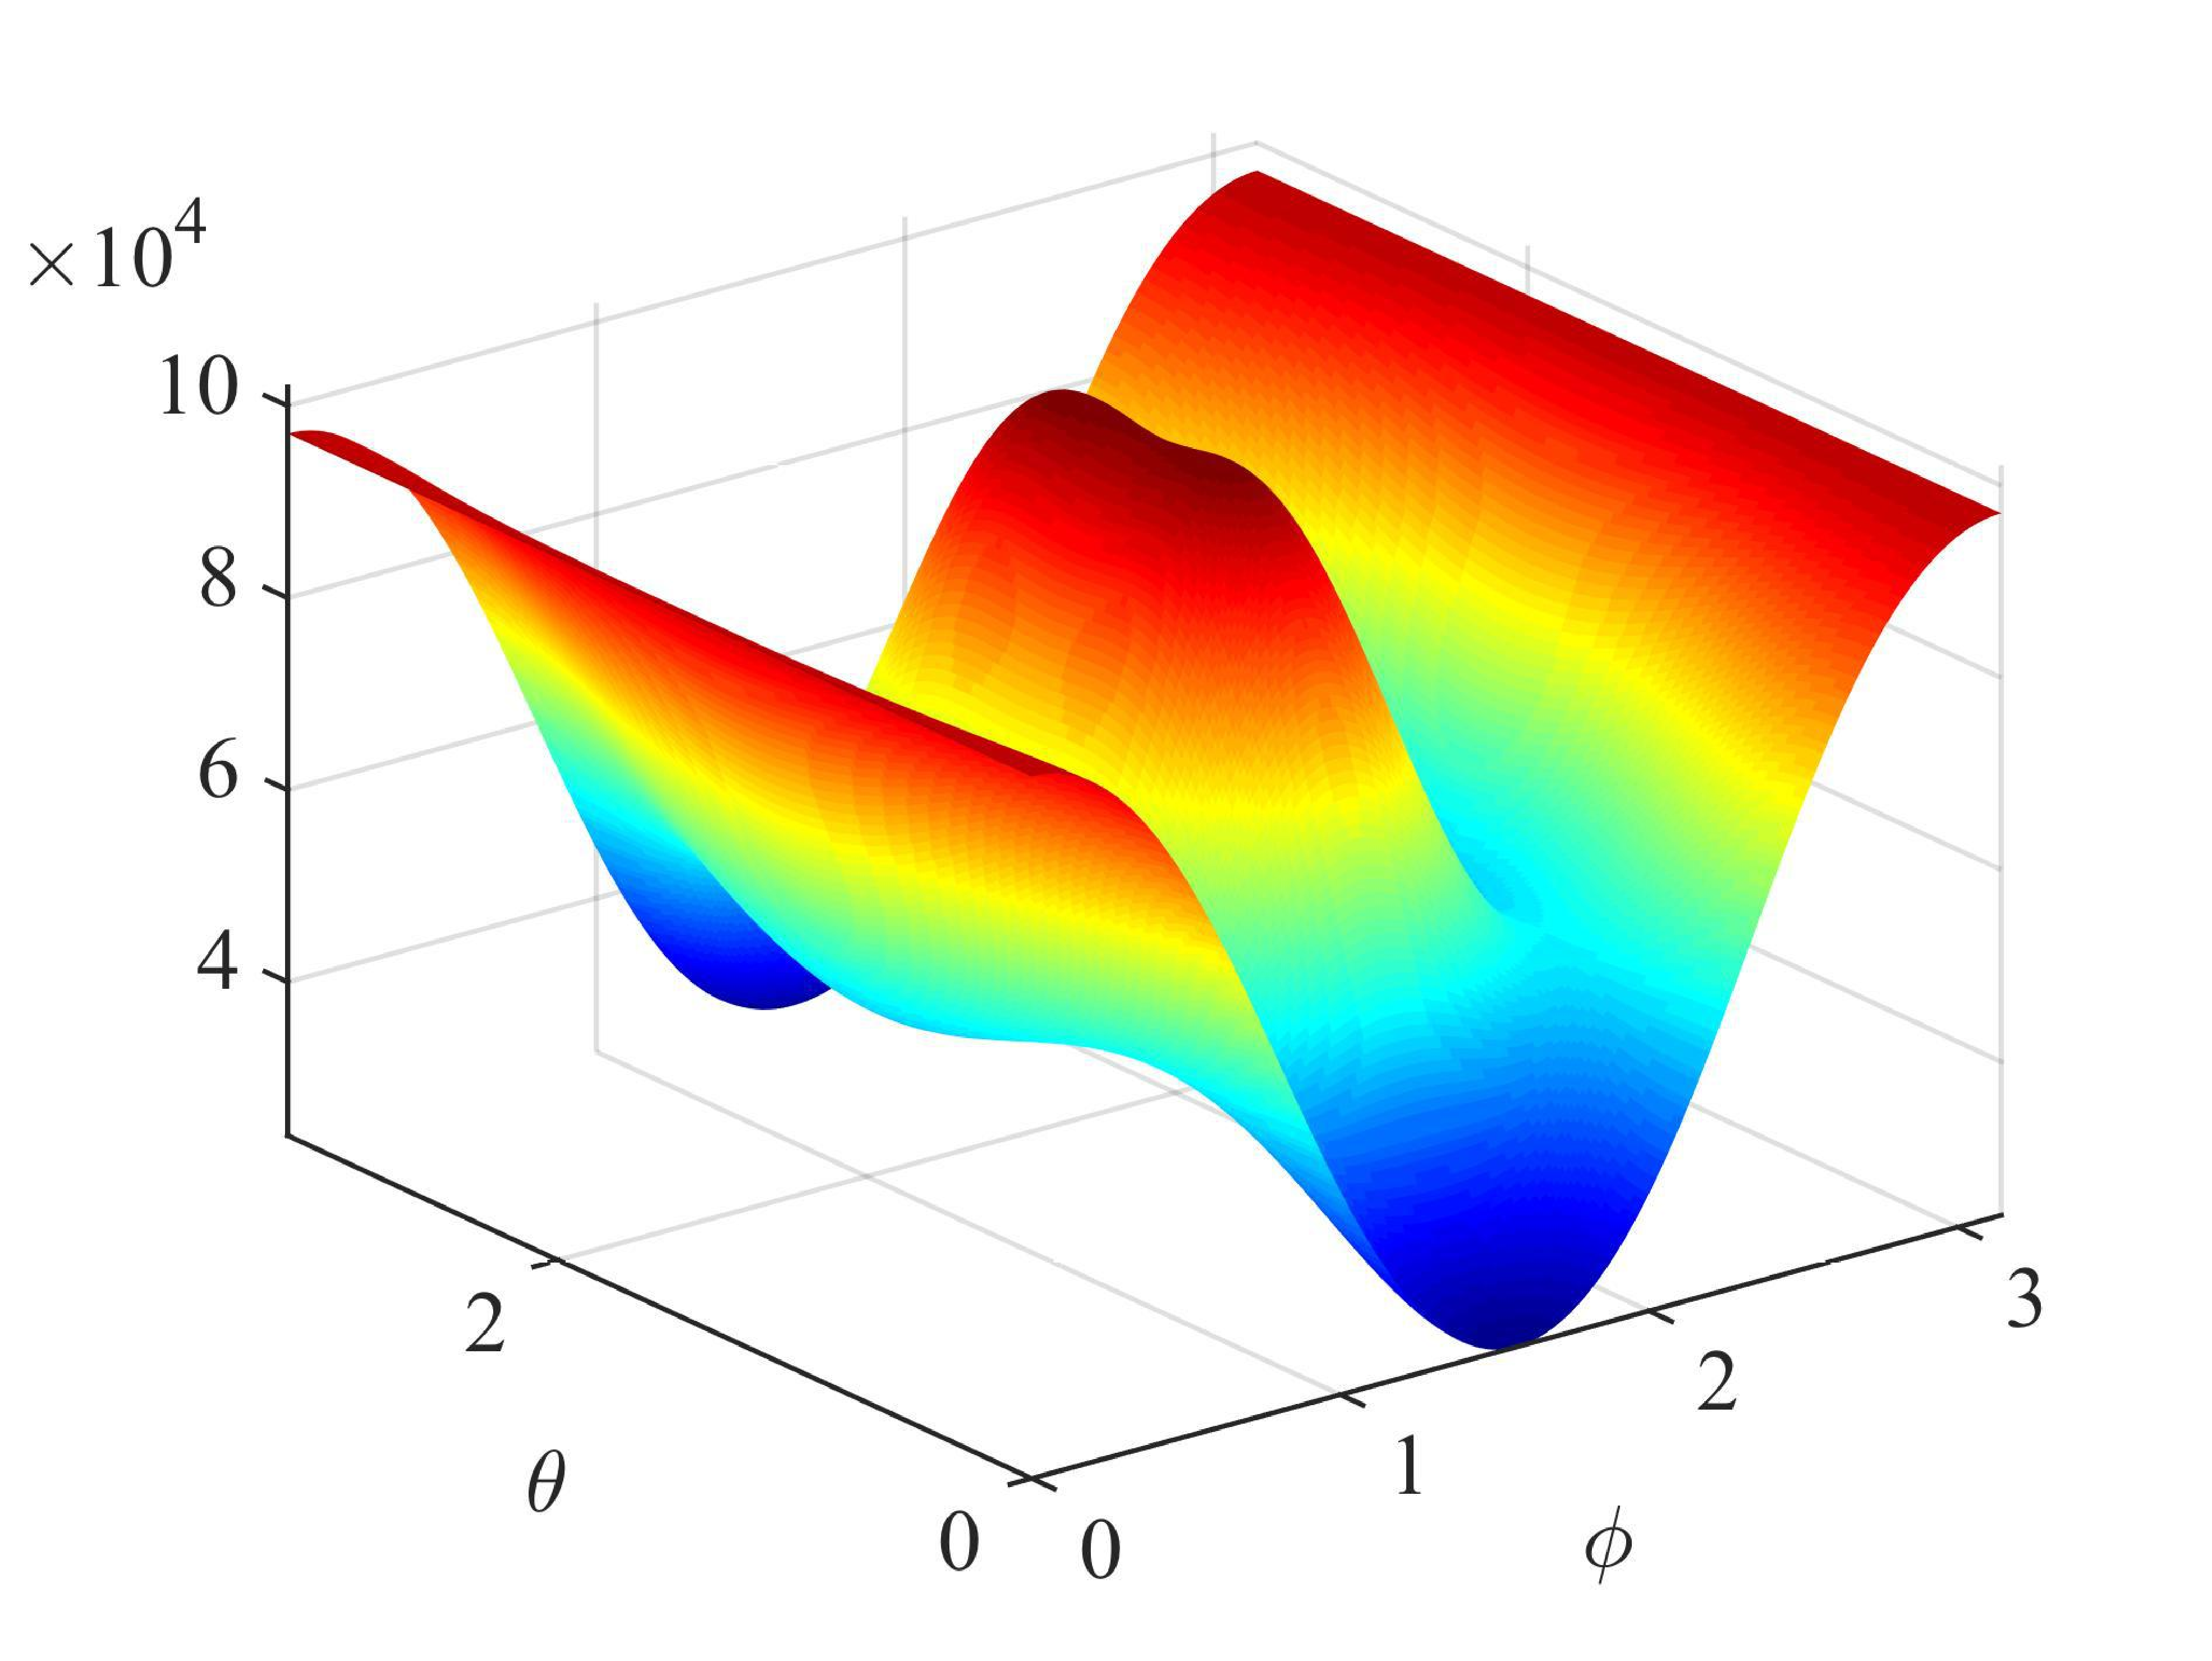
\includegraphics[width=0.45\textwidth]
   {figs/aniso_uniaxial_spherical_detA_F1p1583.pdf}
 } \subfigure[$F_{11}=1.1798$ (bifurcation)]{
   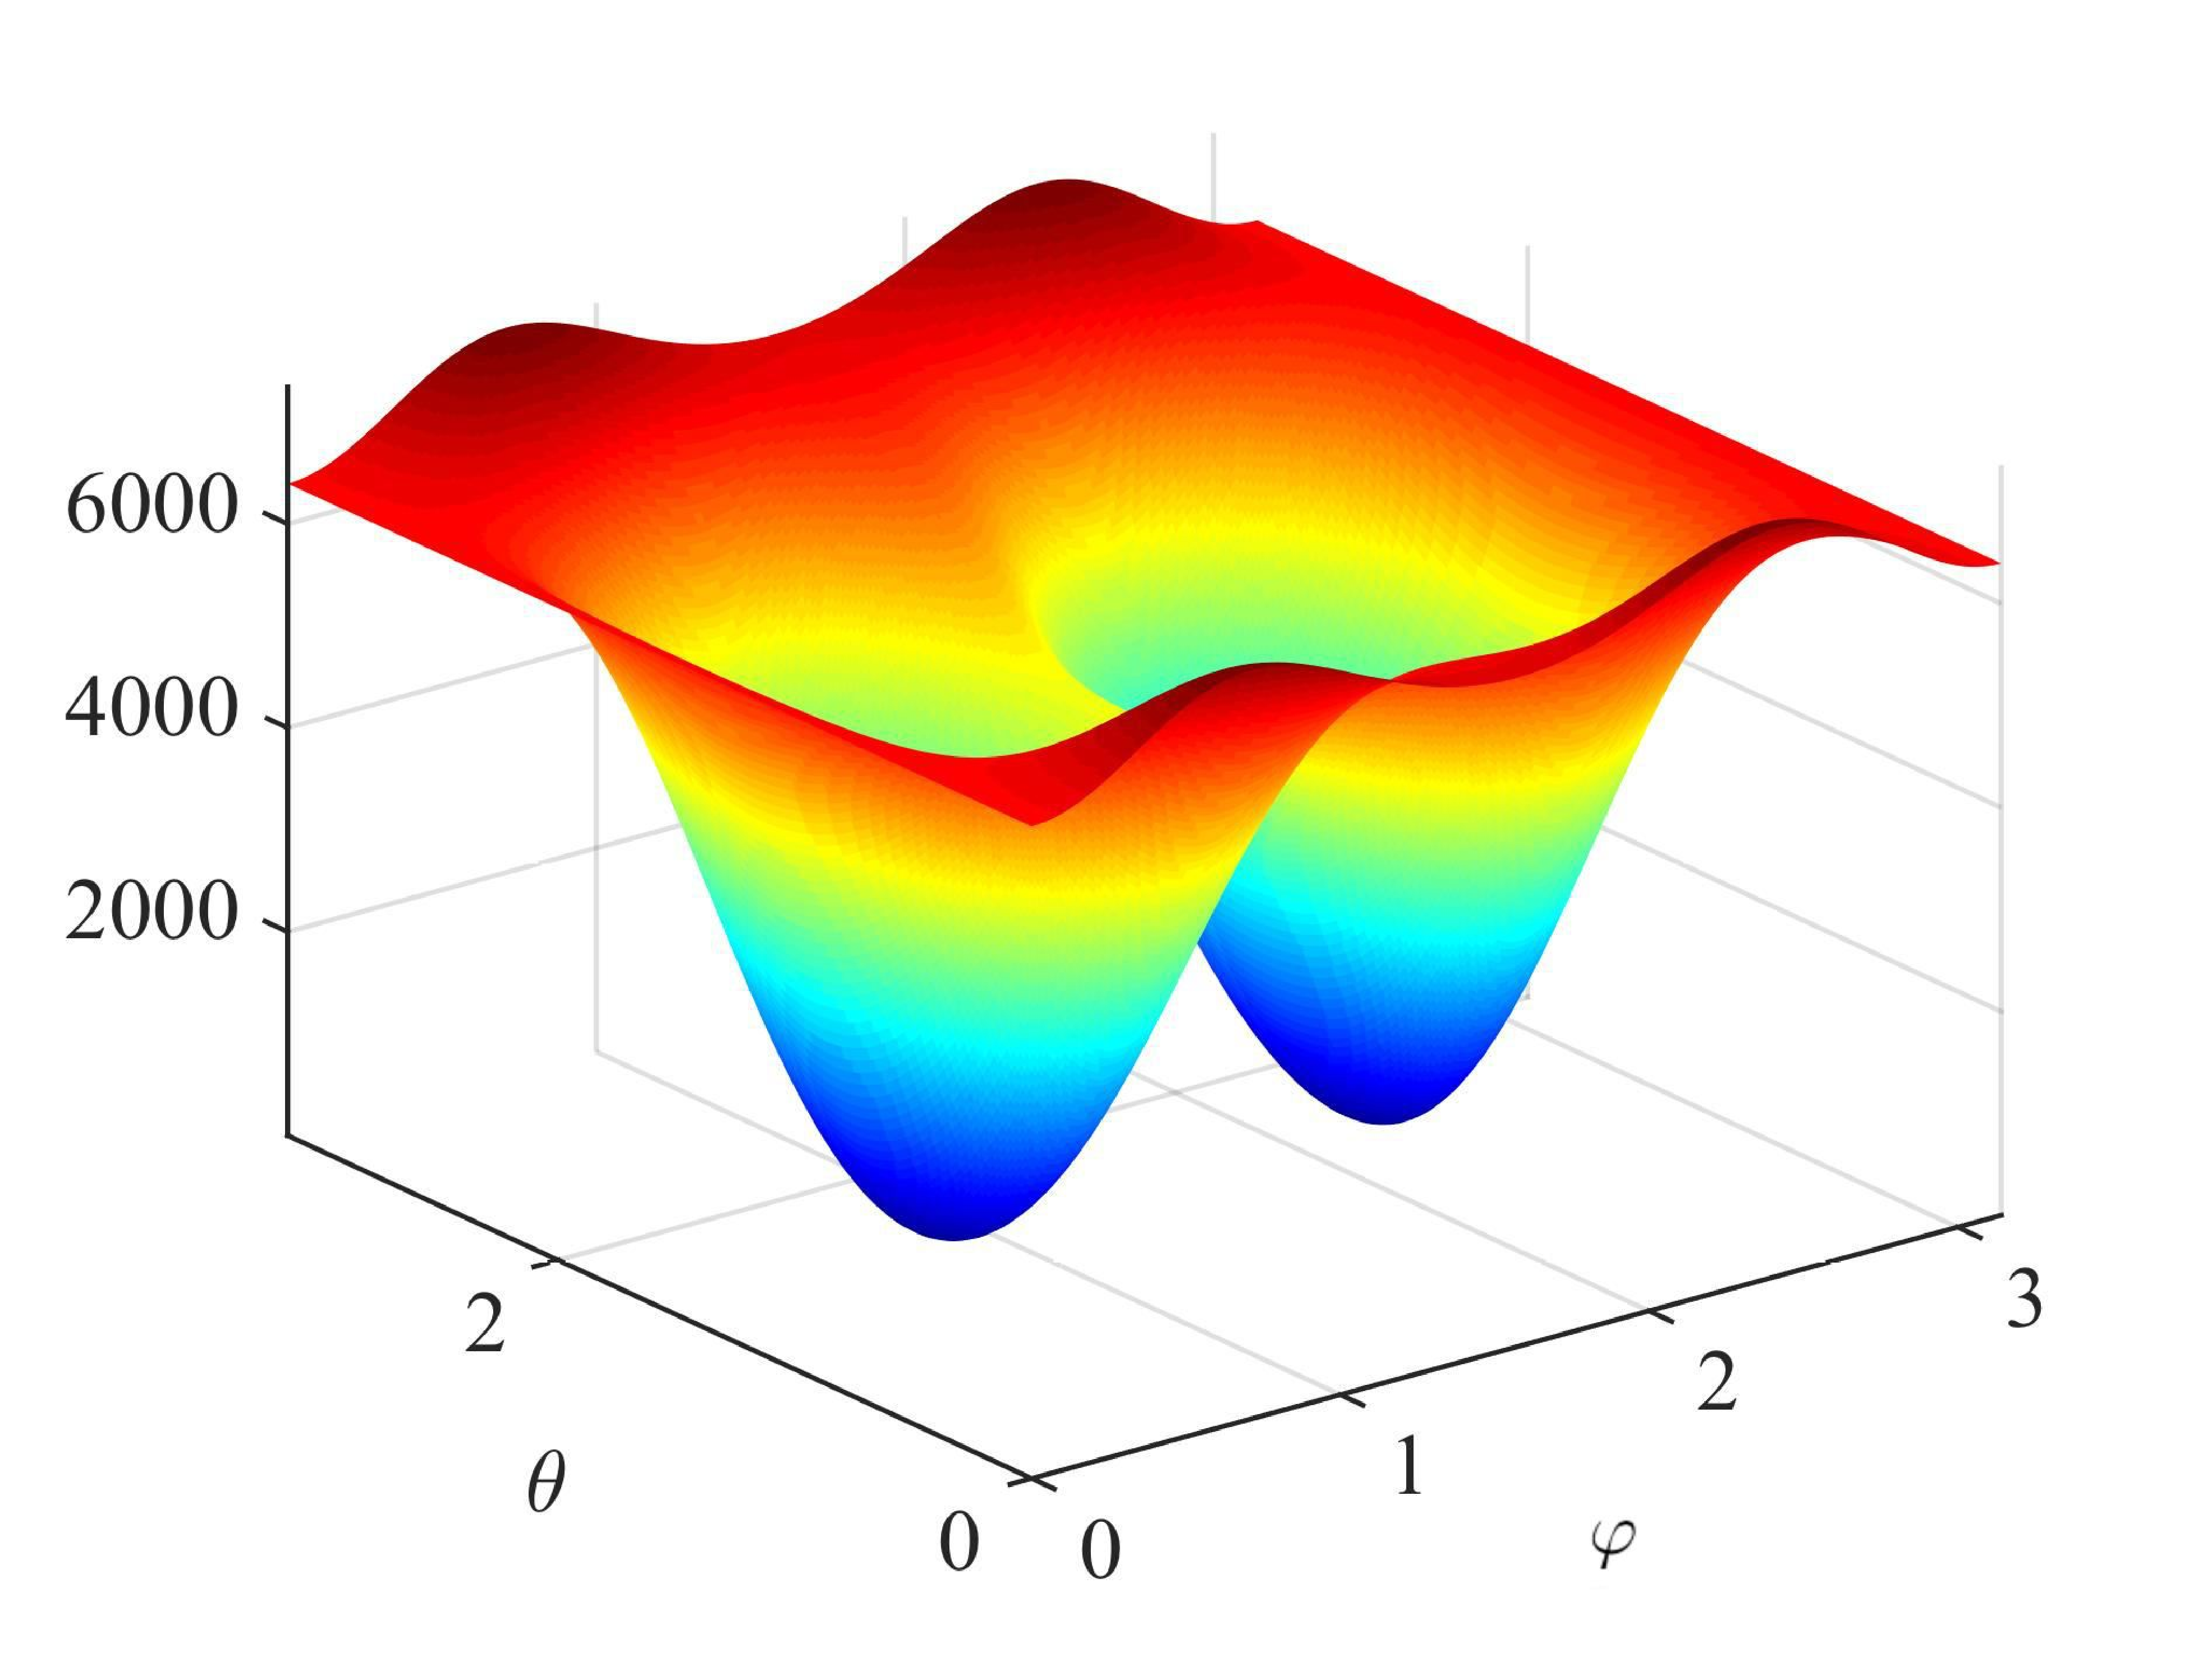
\includegraphics[width=0.45\textwidth]
   {figs/aniso_uniaxial_spherical_detA_F1p1798.pdf}
 }
   \caption{Spherical parametrization: landscapes of $\det~A$ for the
     uniaxial tension test of the finite deformation anisotropic model
     at different axial stretch levels.}
   \label{fig:aniso-spherical-detA}
 \end{figure}

\begin{figure}[!htbp]
   \centering \subfigure[$F_{11}=1.0074$]{
   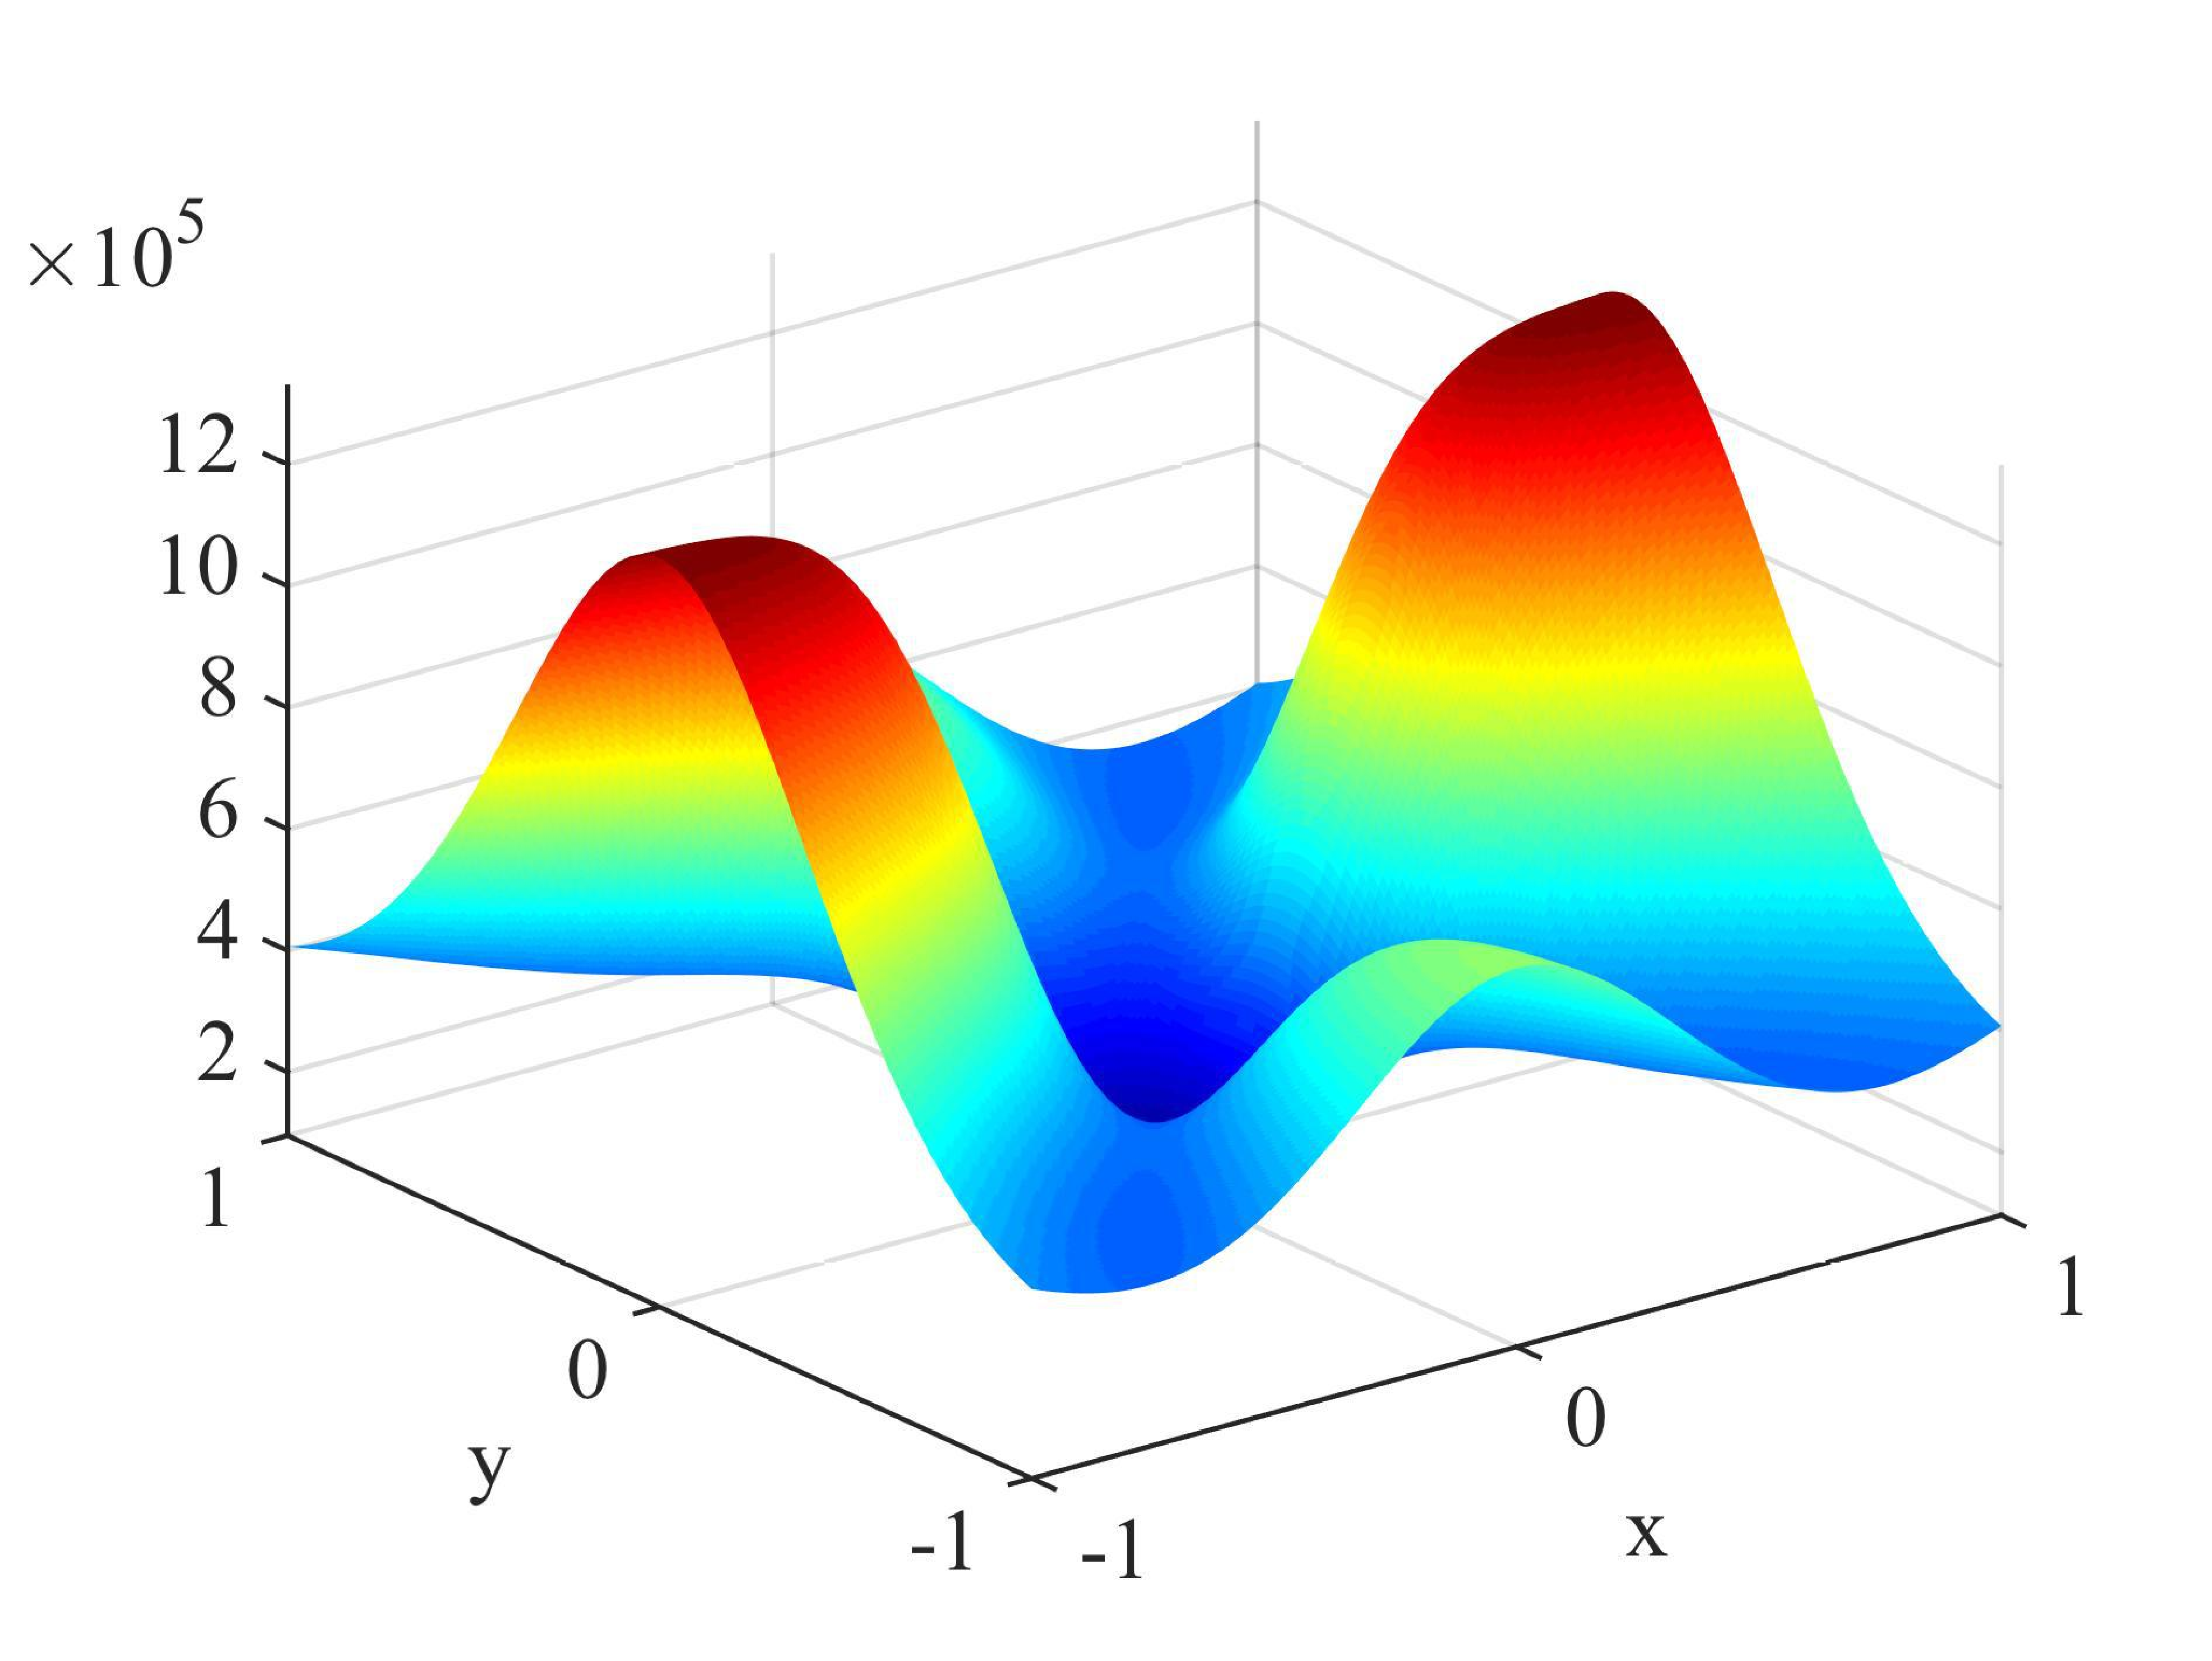
\includegraphics[width=0.45\textwidth]
   {figs/aniso_uniaxial_stereographic_detA_F1p0074.pdf}
 } \subfigure[$F_{11}=1.0762$]{
   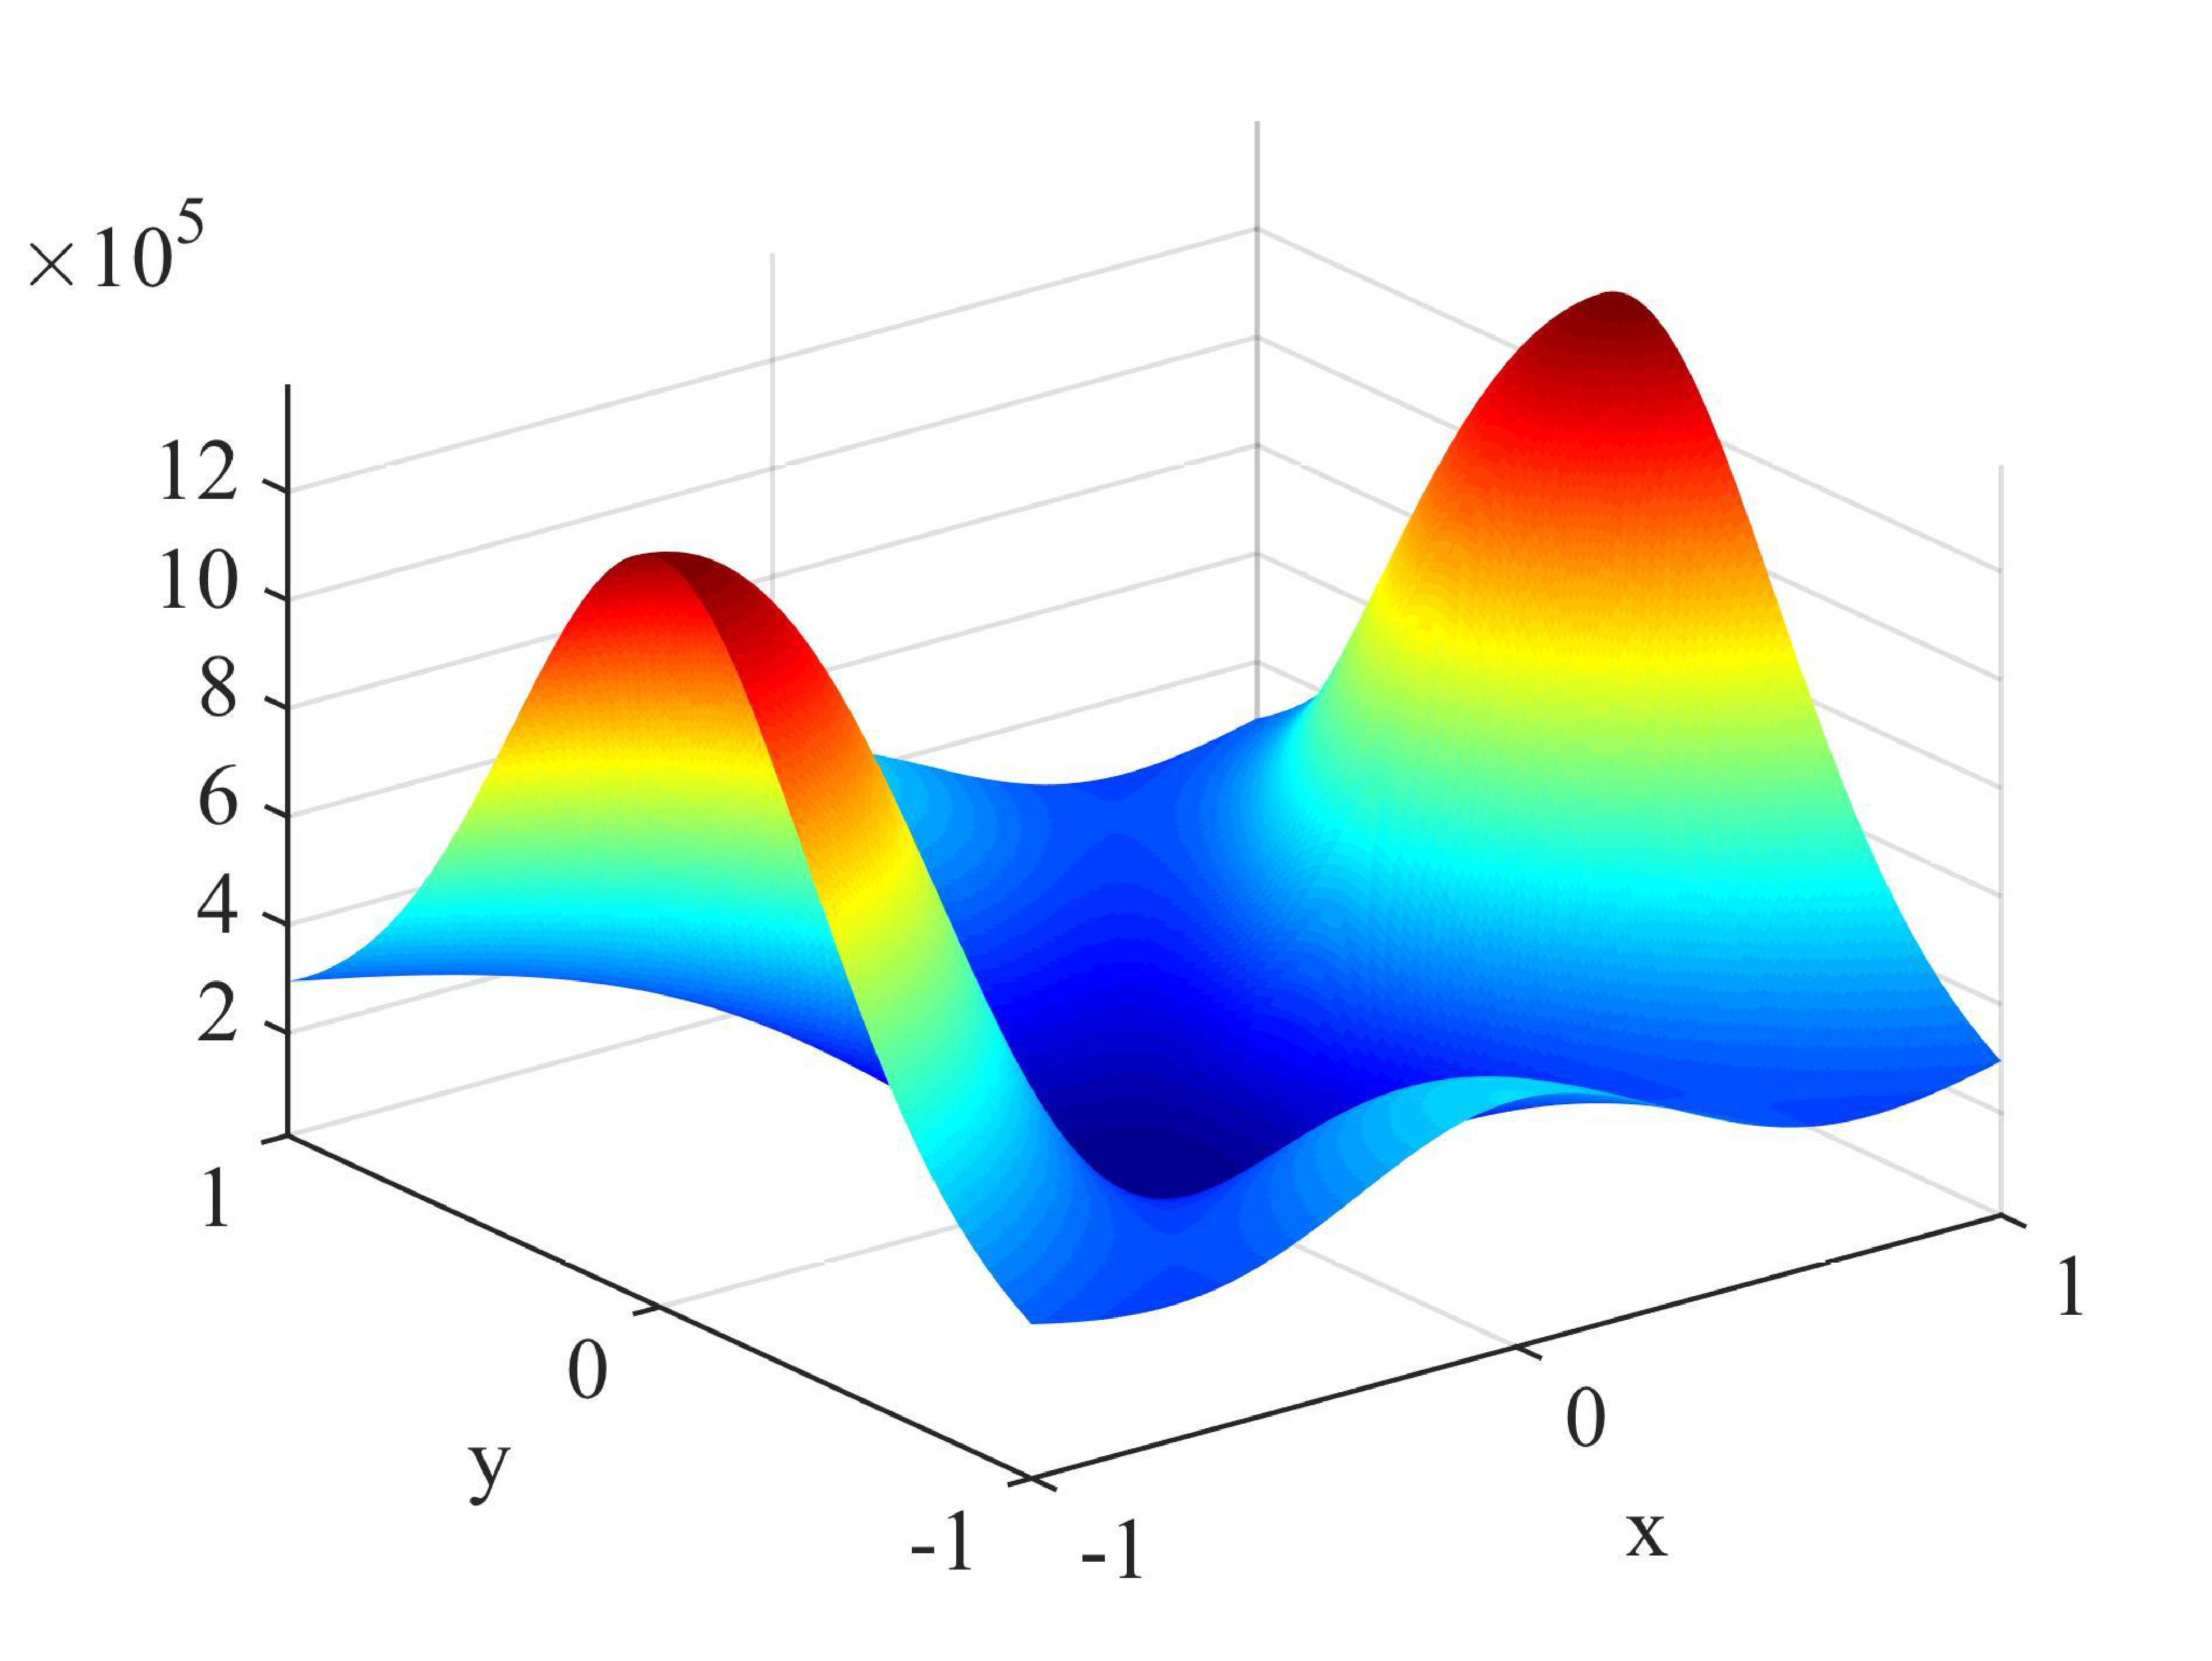
\includegraphics[width=0.45\textwidth]
   {figs/aniso_uniaxial_stereographic_detA_F1p0762.pdf}
 } \subfigure[$F_{11}=1.1583$]{
   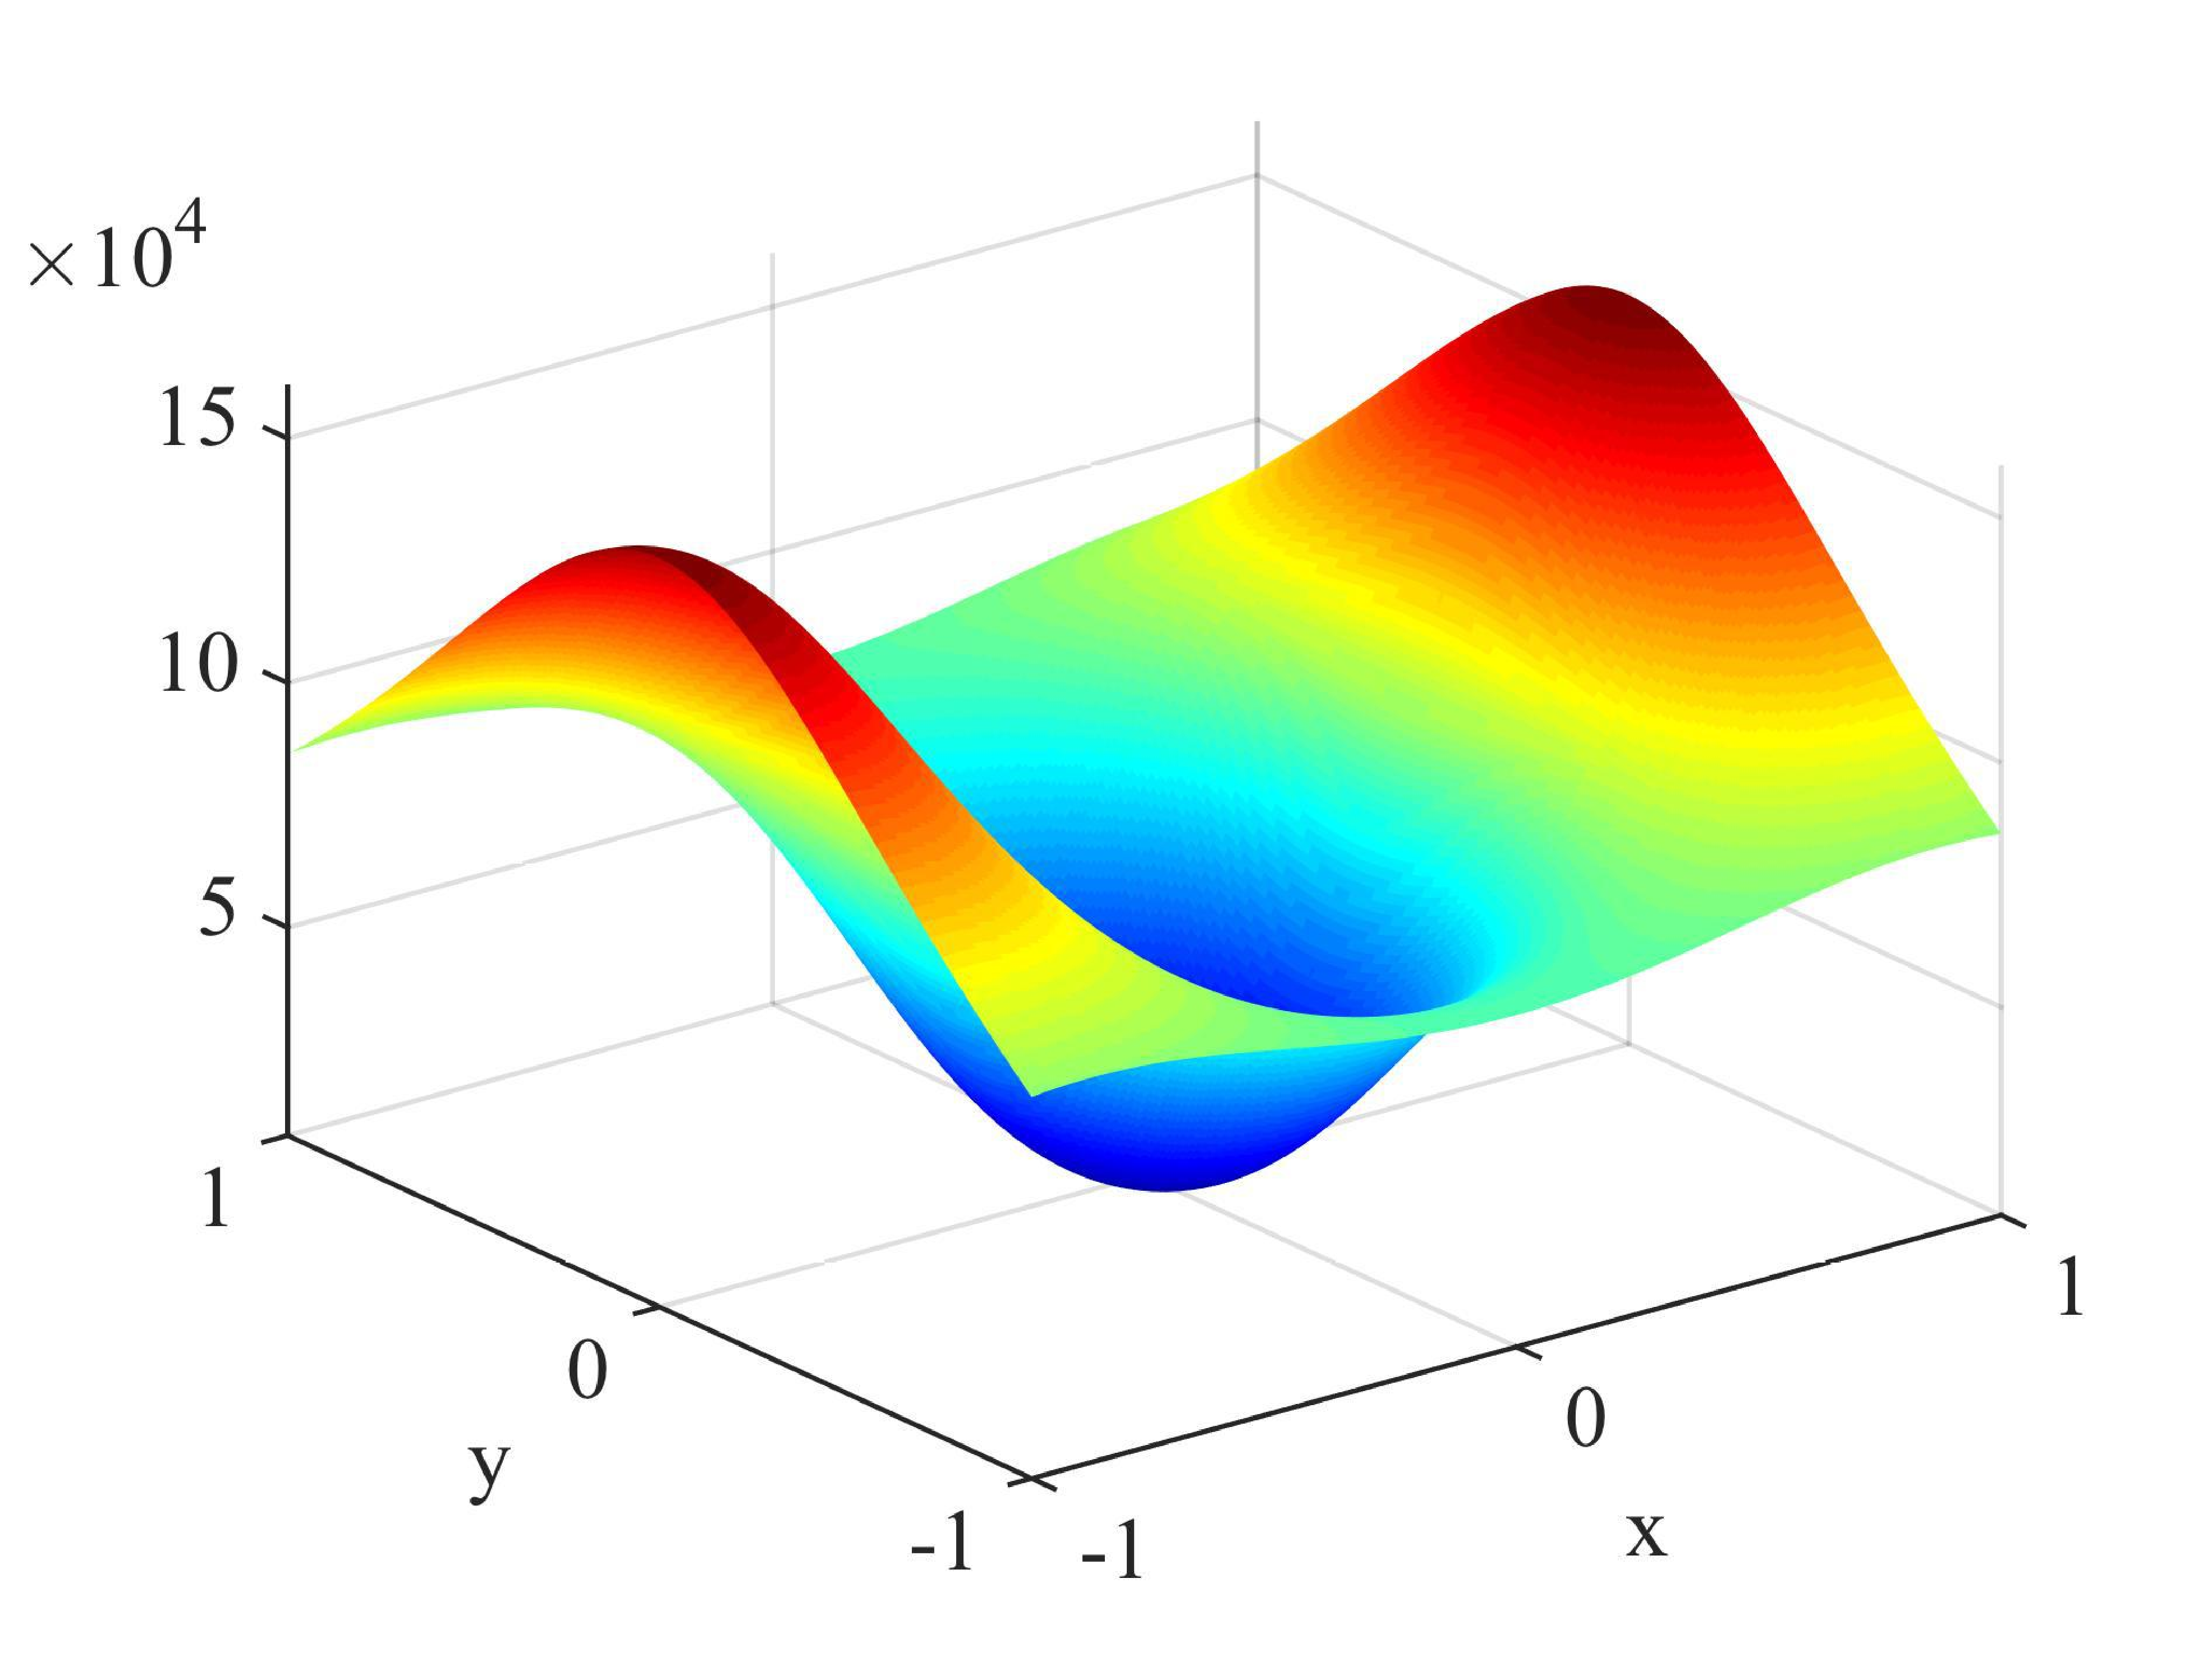
\includegraphics[width=0.45\textwidth]
   {figs/aniso_uniaxial_stereographic_detA_F1p1583.pdf}
 } \subfigure[$F_{11}=1.1798$ (bifurcation)]{
   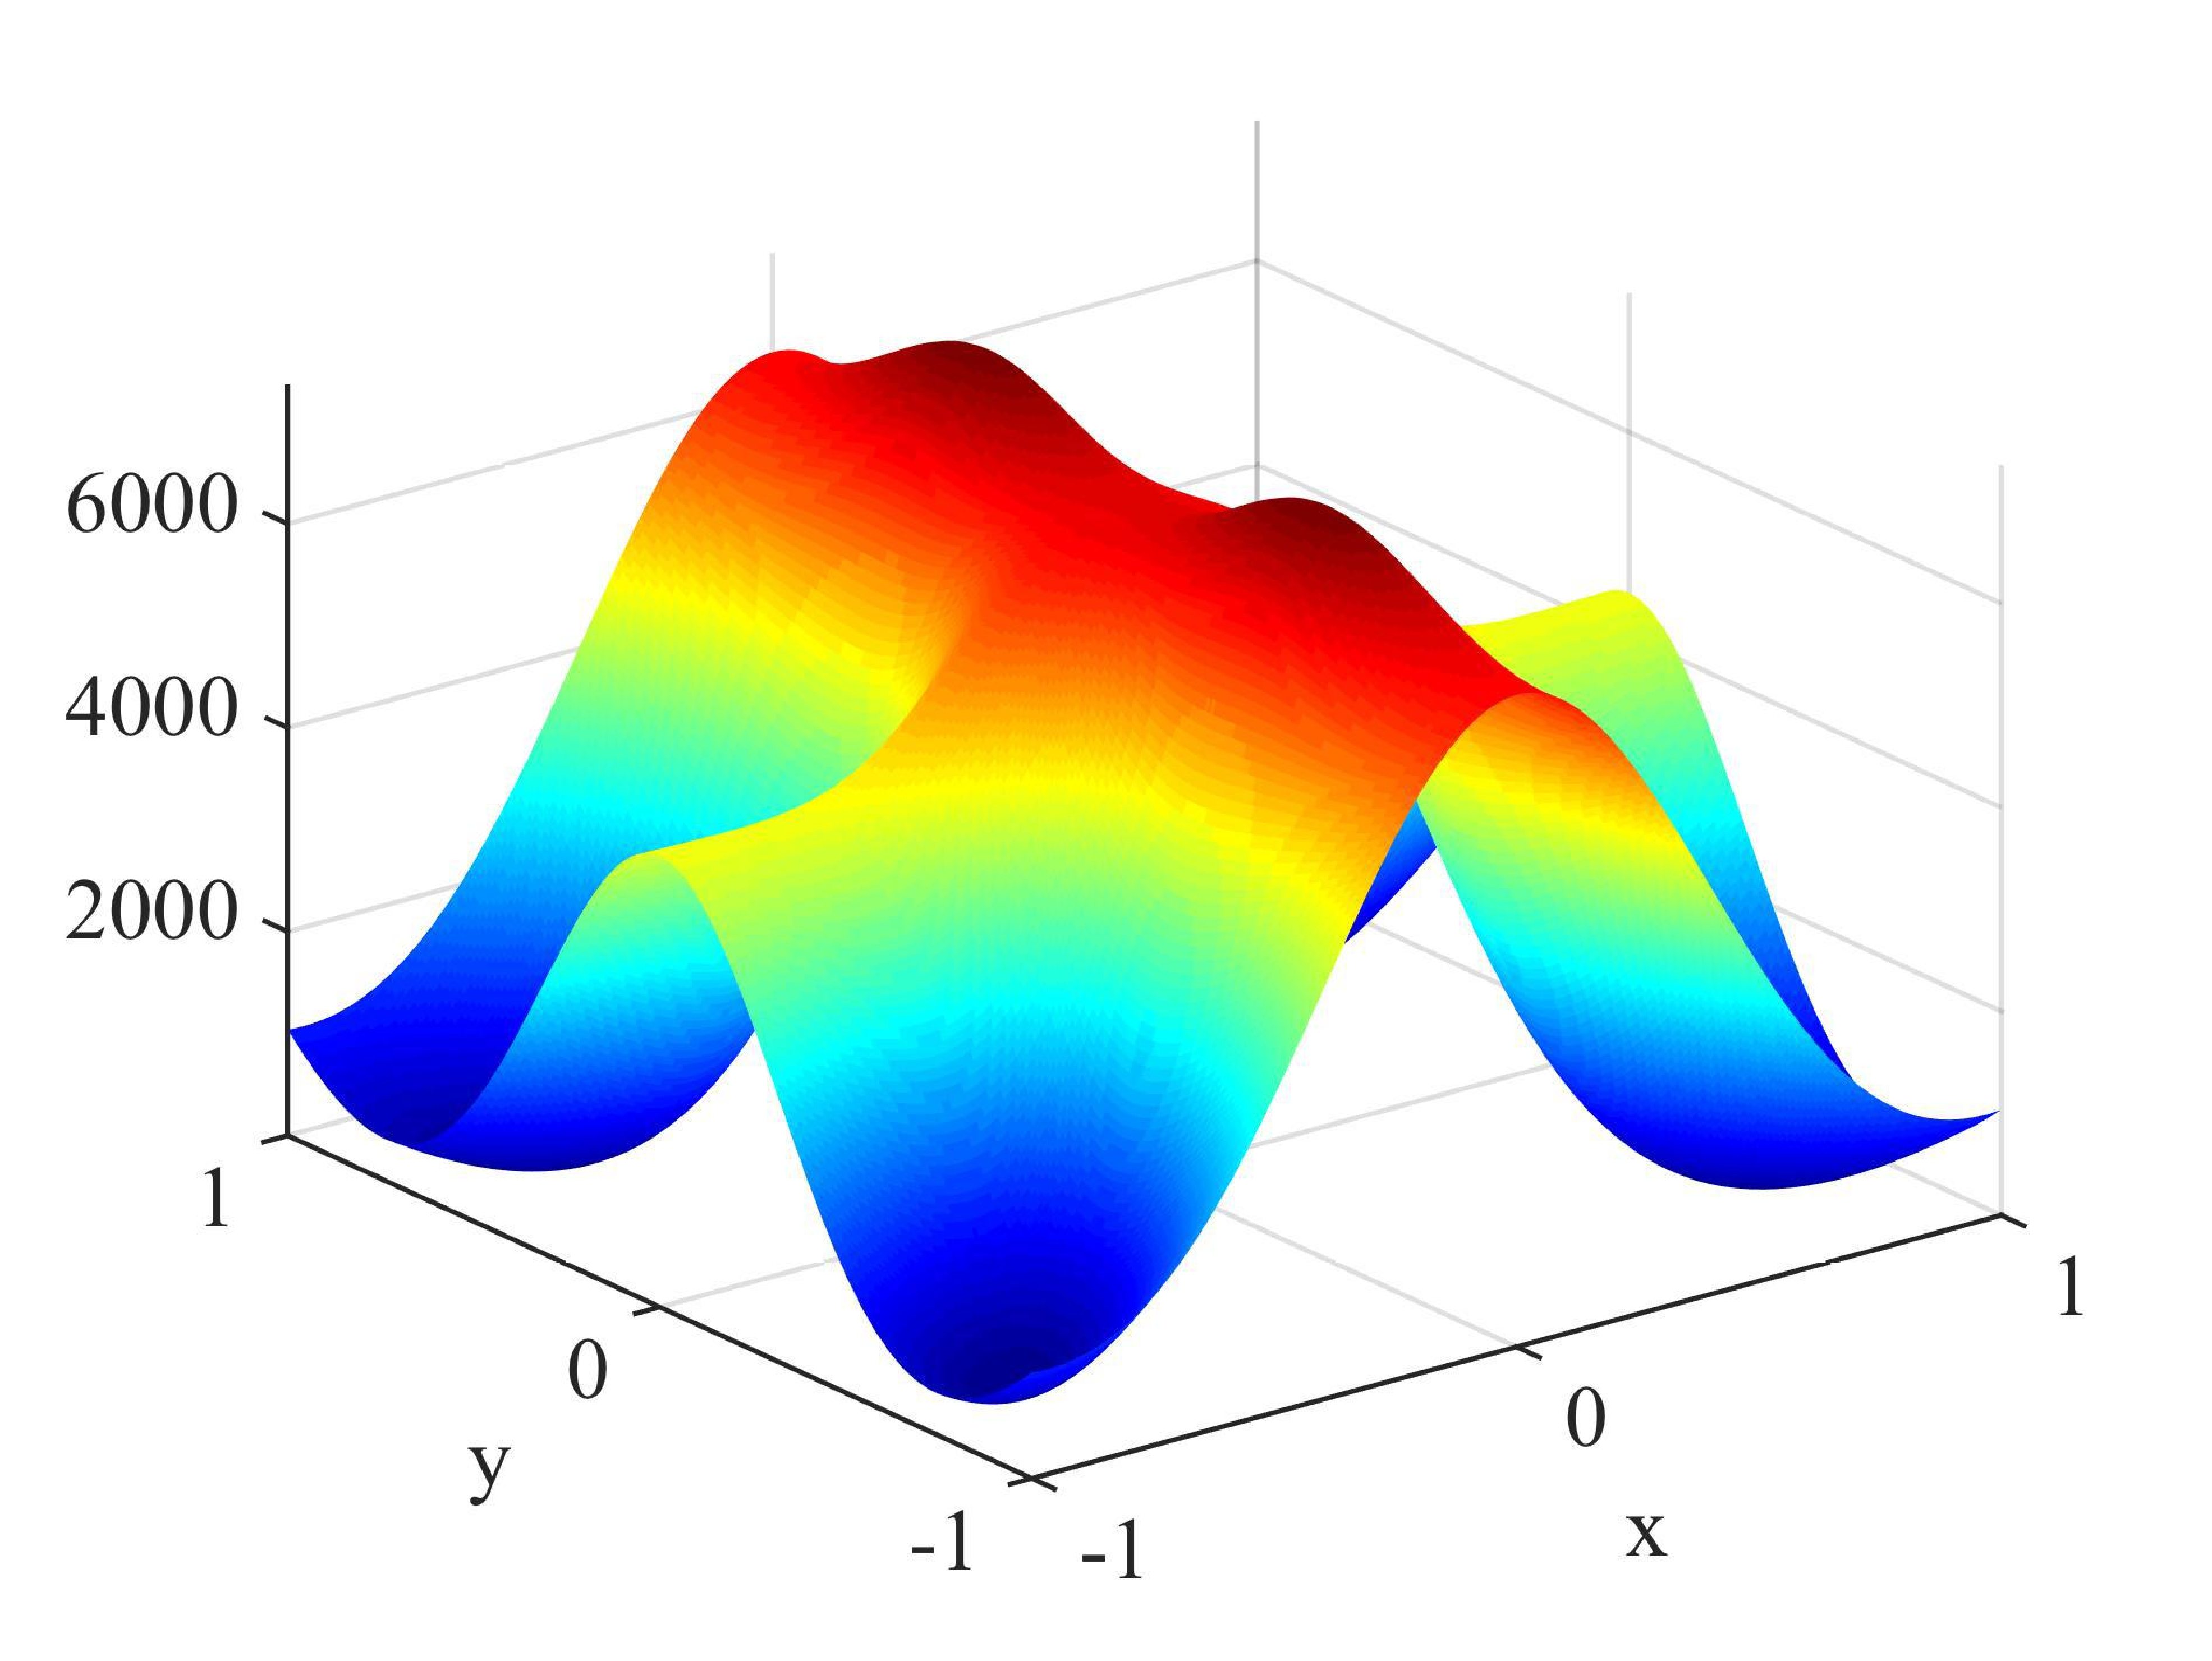
\includegraphics[width=0.45\textwidth]
   {figs/aniso_uniaxial_stereographic_detA_F1p1798.pdf}
 }
   \caption{Stereographic parametrization: landscapes of $\det~A$ for
     the uniaxial tension test of the finite deformation anisotropic
     model at different axial stretch levels.}
   \label{fig:aniso-stereographic-detA}
 \end{figure}

\begin{figure}[!htbp]
   \centering \subfigure[$F_{11}=1.0074$]{
   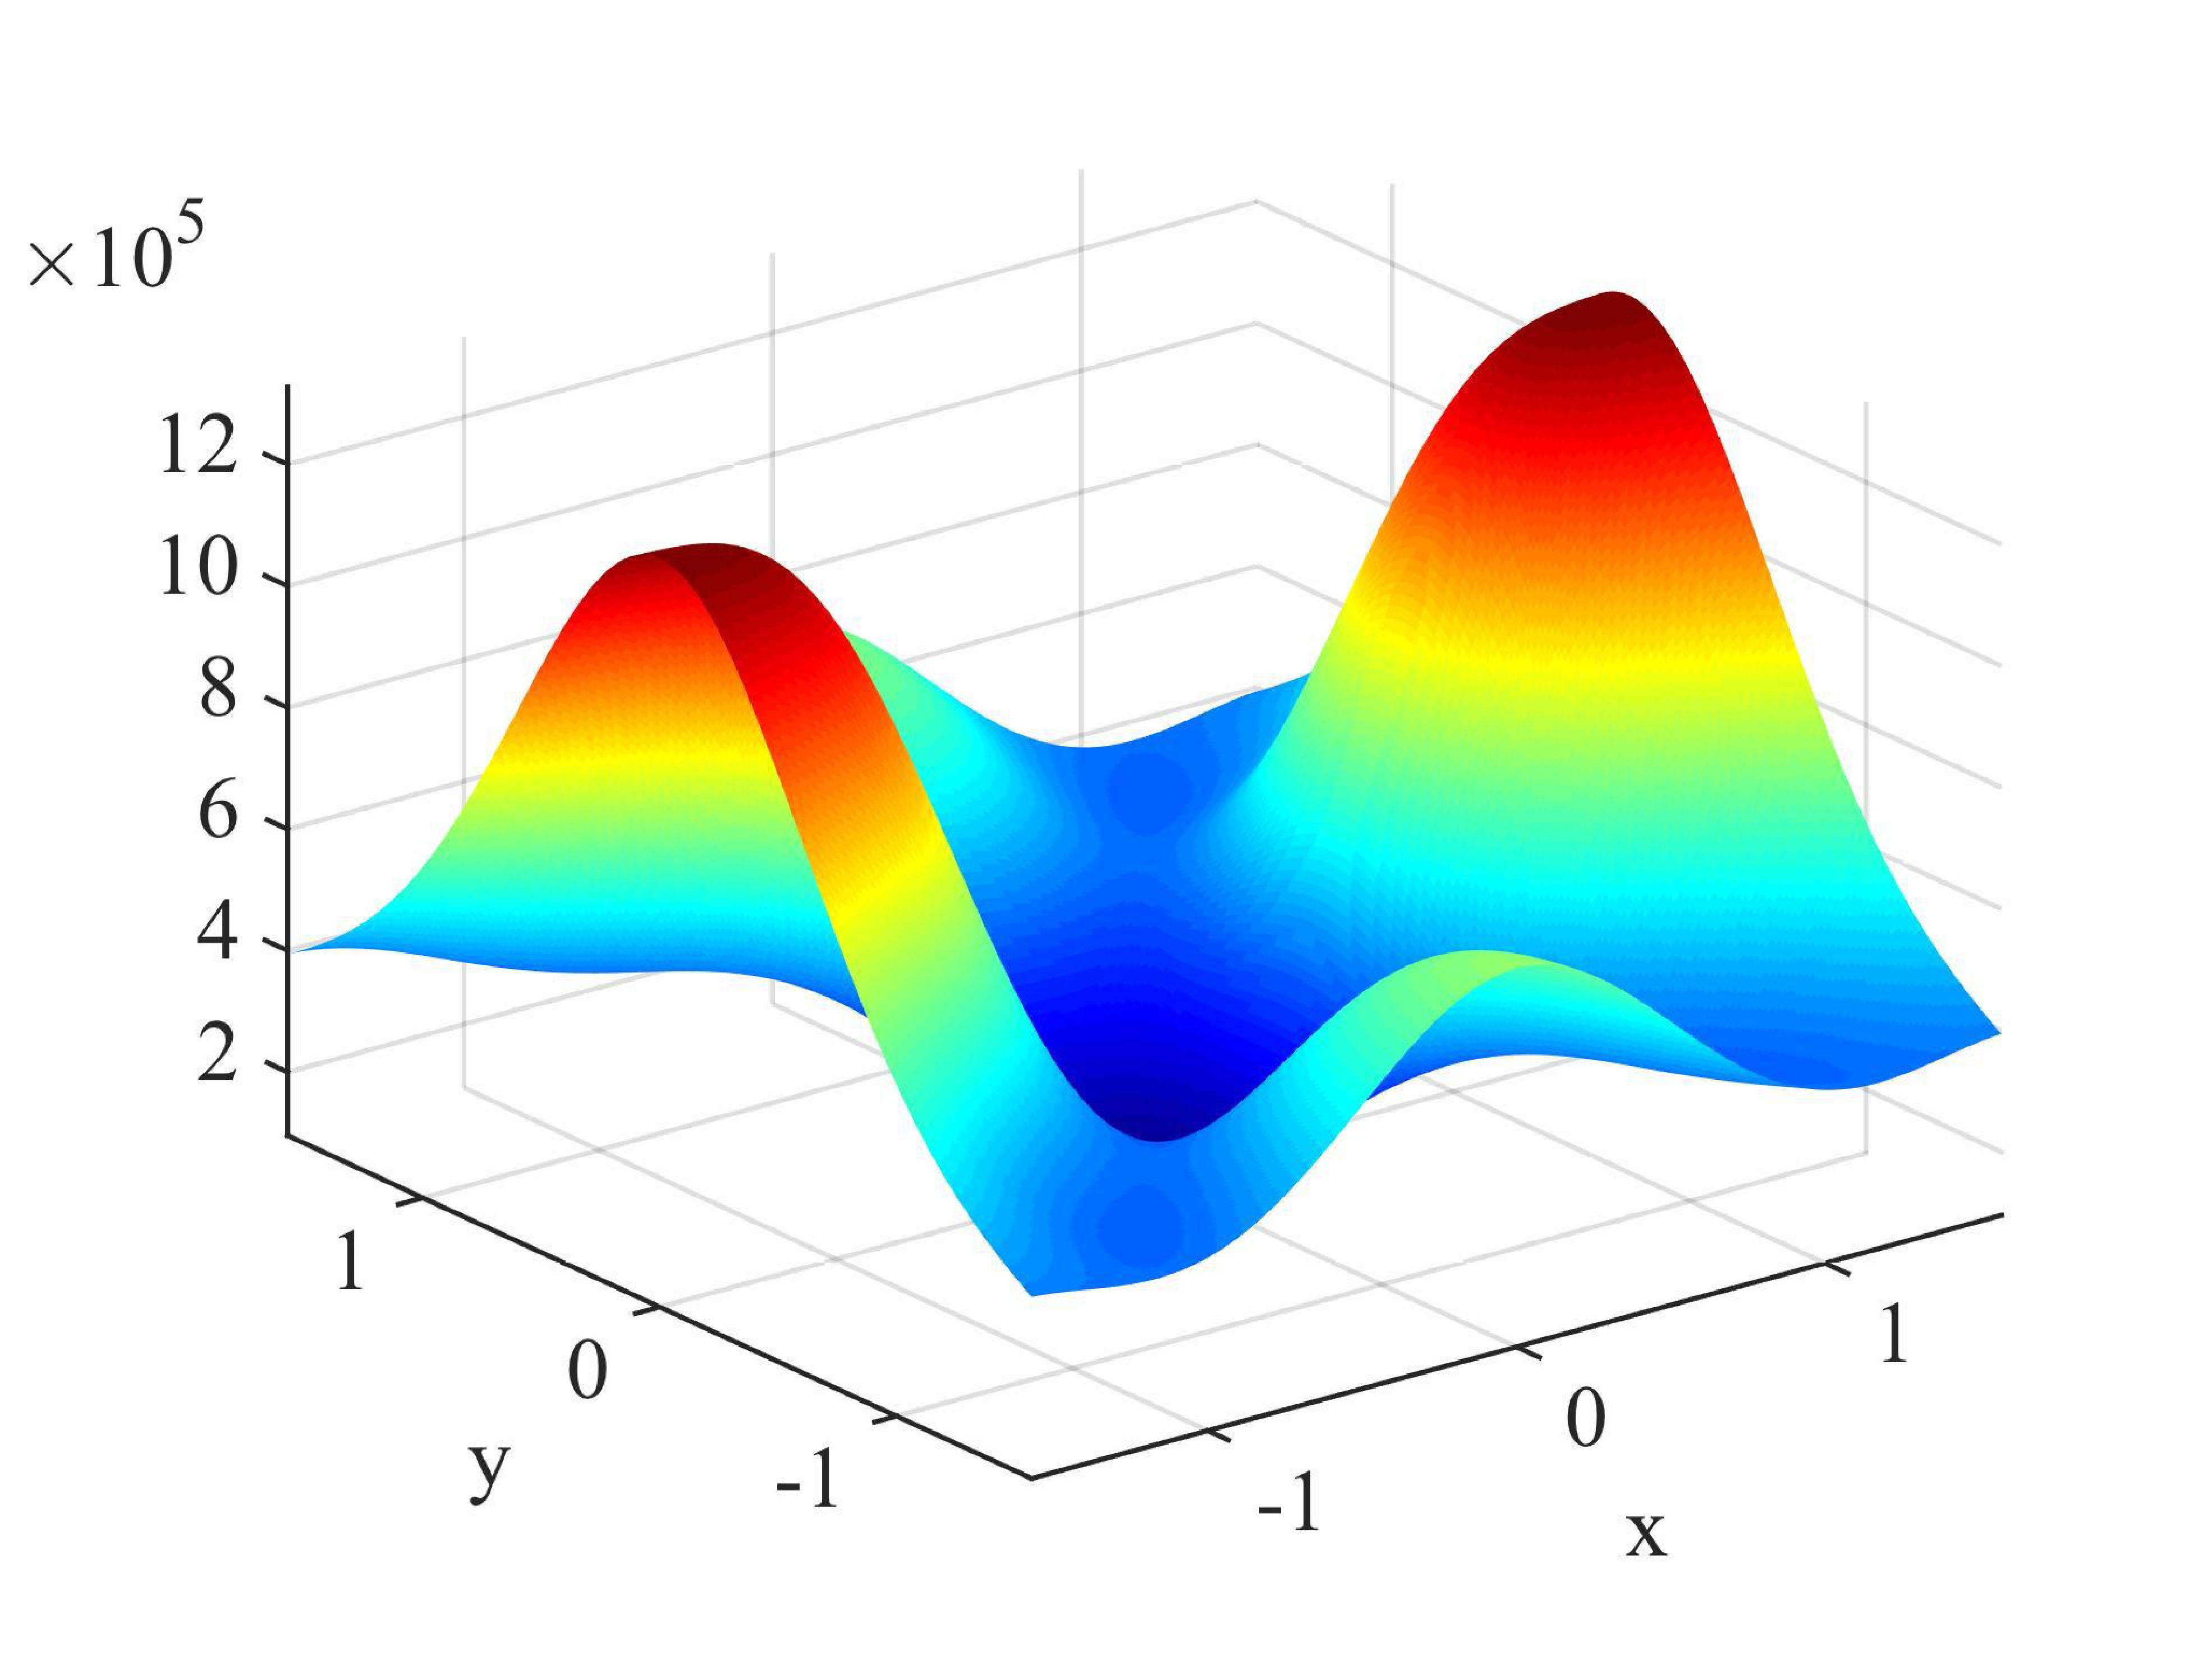
\includegraphics[width=0.45\textwidth]
   {figs/aniso_uniaxial_tangent_detA_F1p0074.pdf}
 } \subfigure[$F_{11}=1.0762$]{
   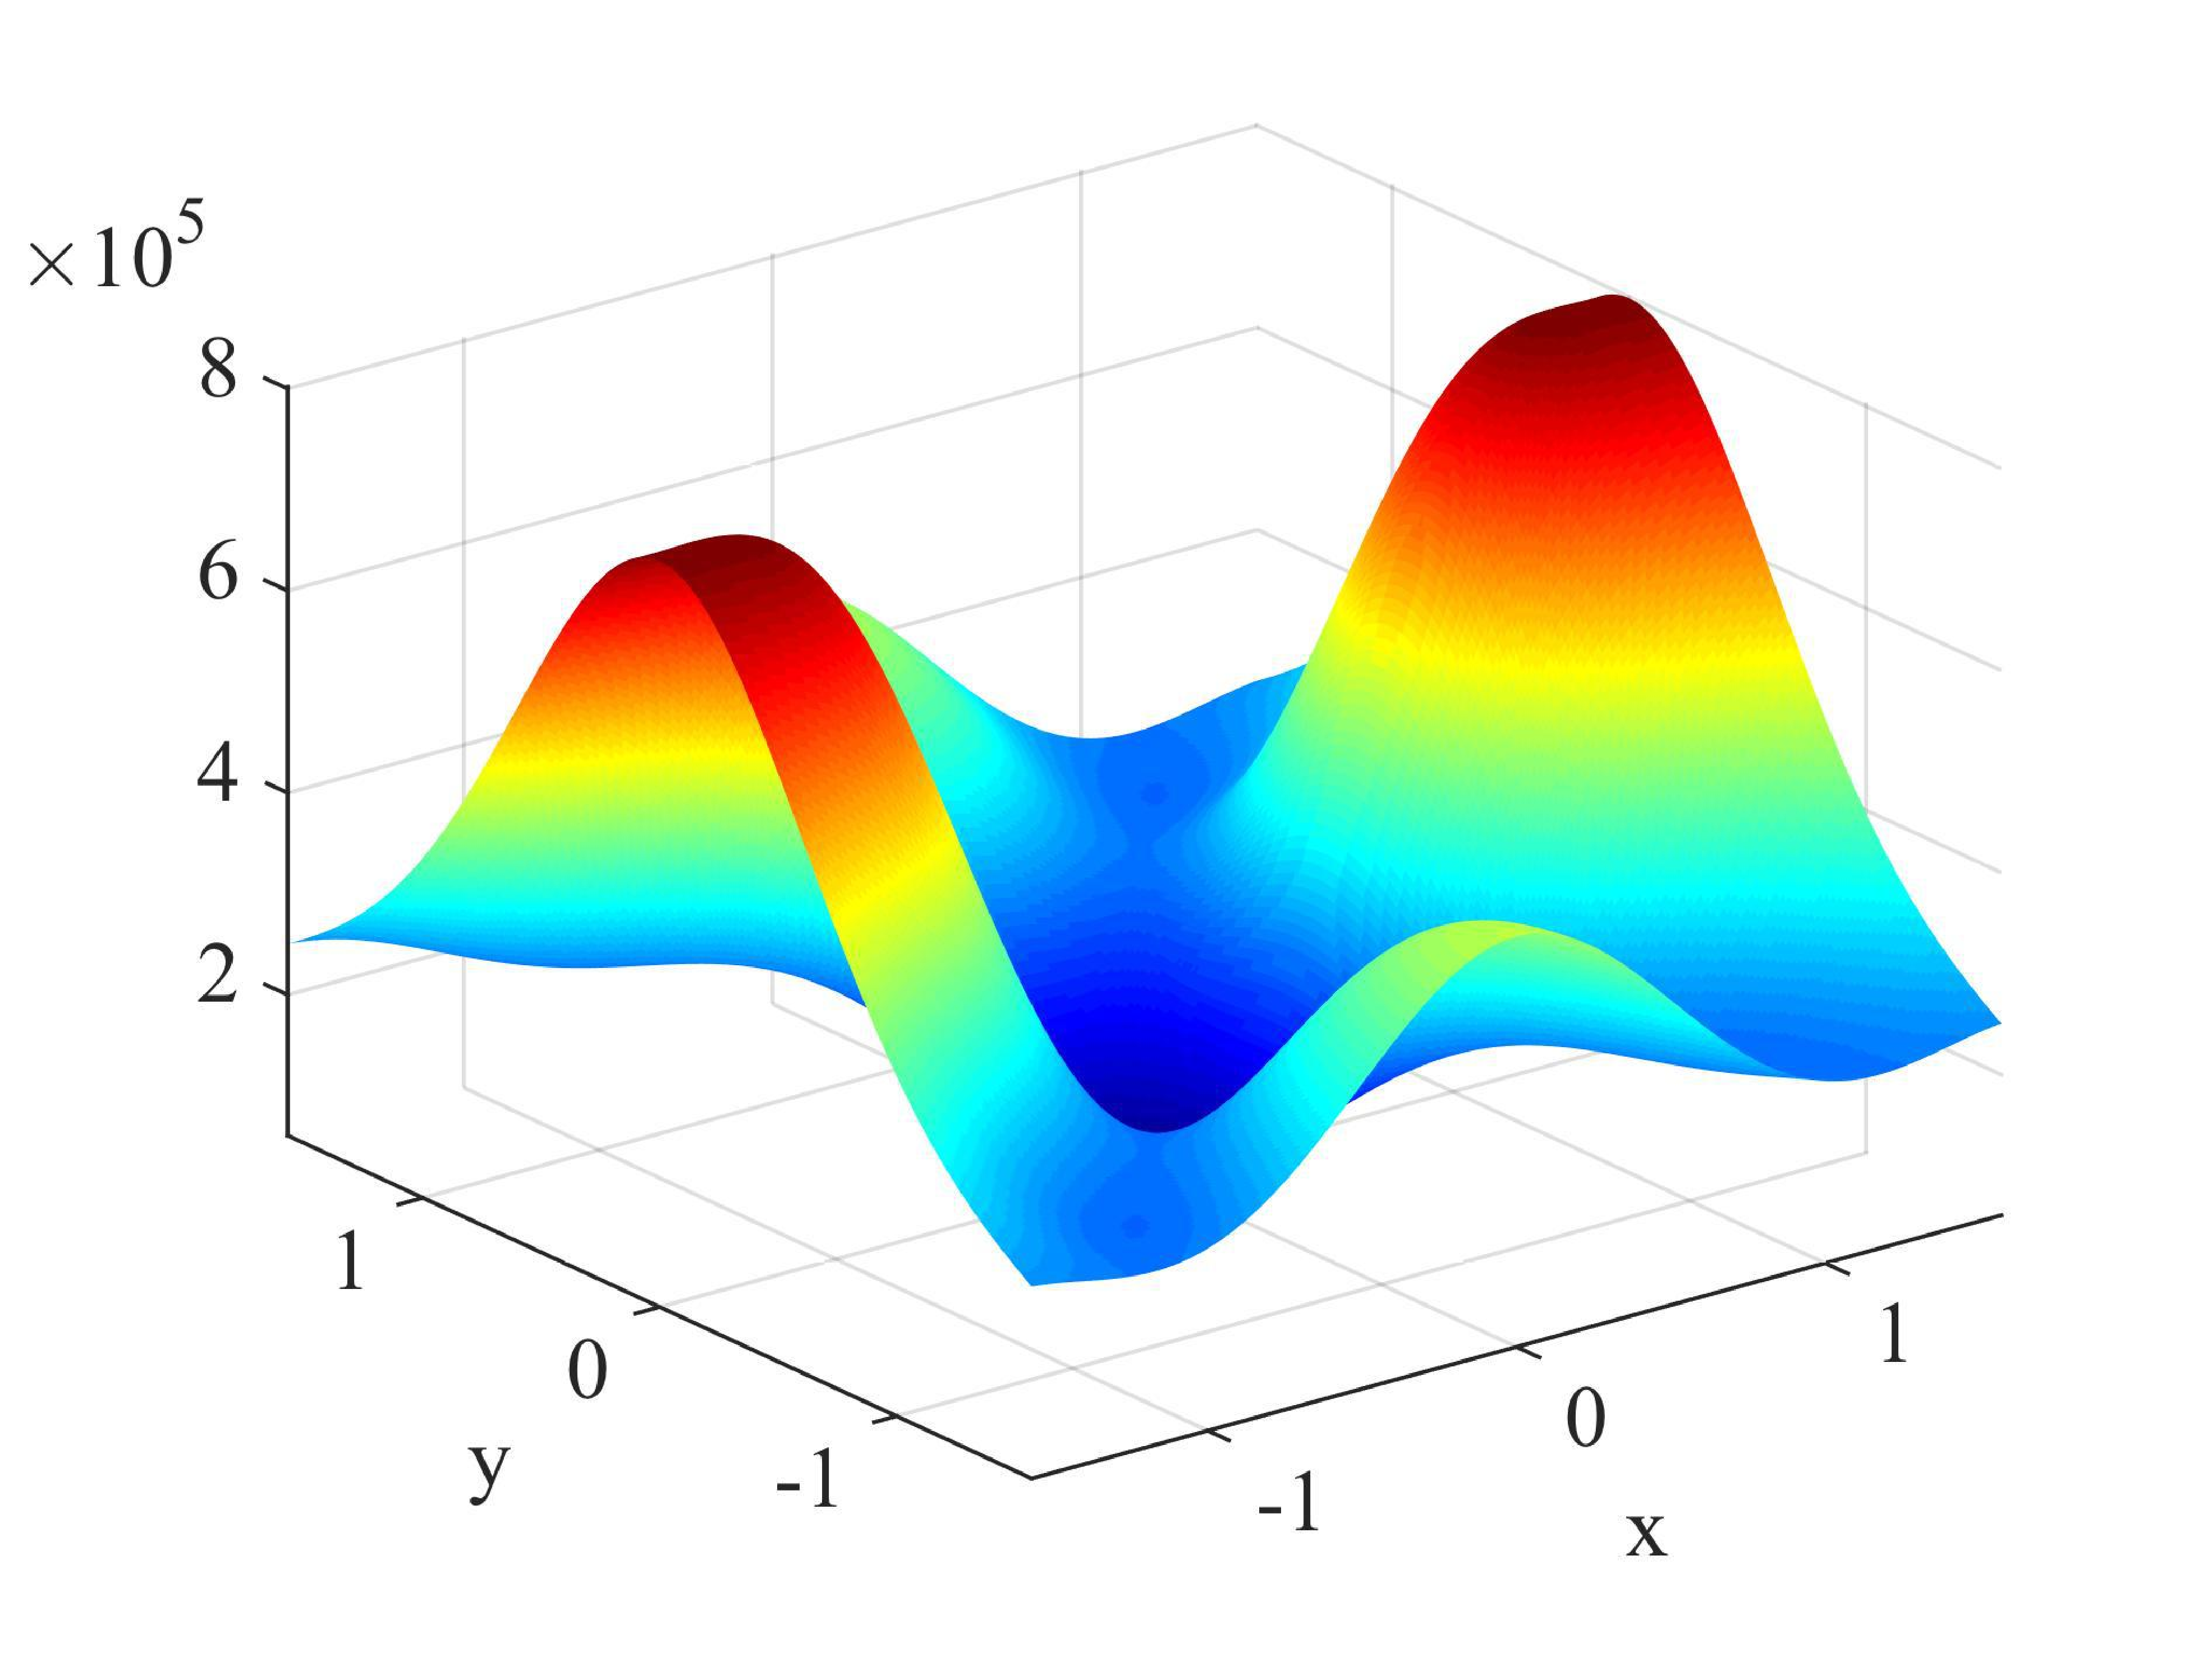
\includegraphics[width=0.45\textwidth]
   {figs/aniso_uniaxial_tangent_detA_F1p0762.pdf}
 } \subfigure[$F_{11}=1.1583$]{
   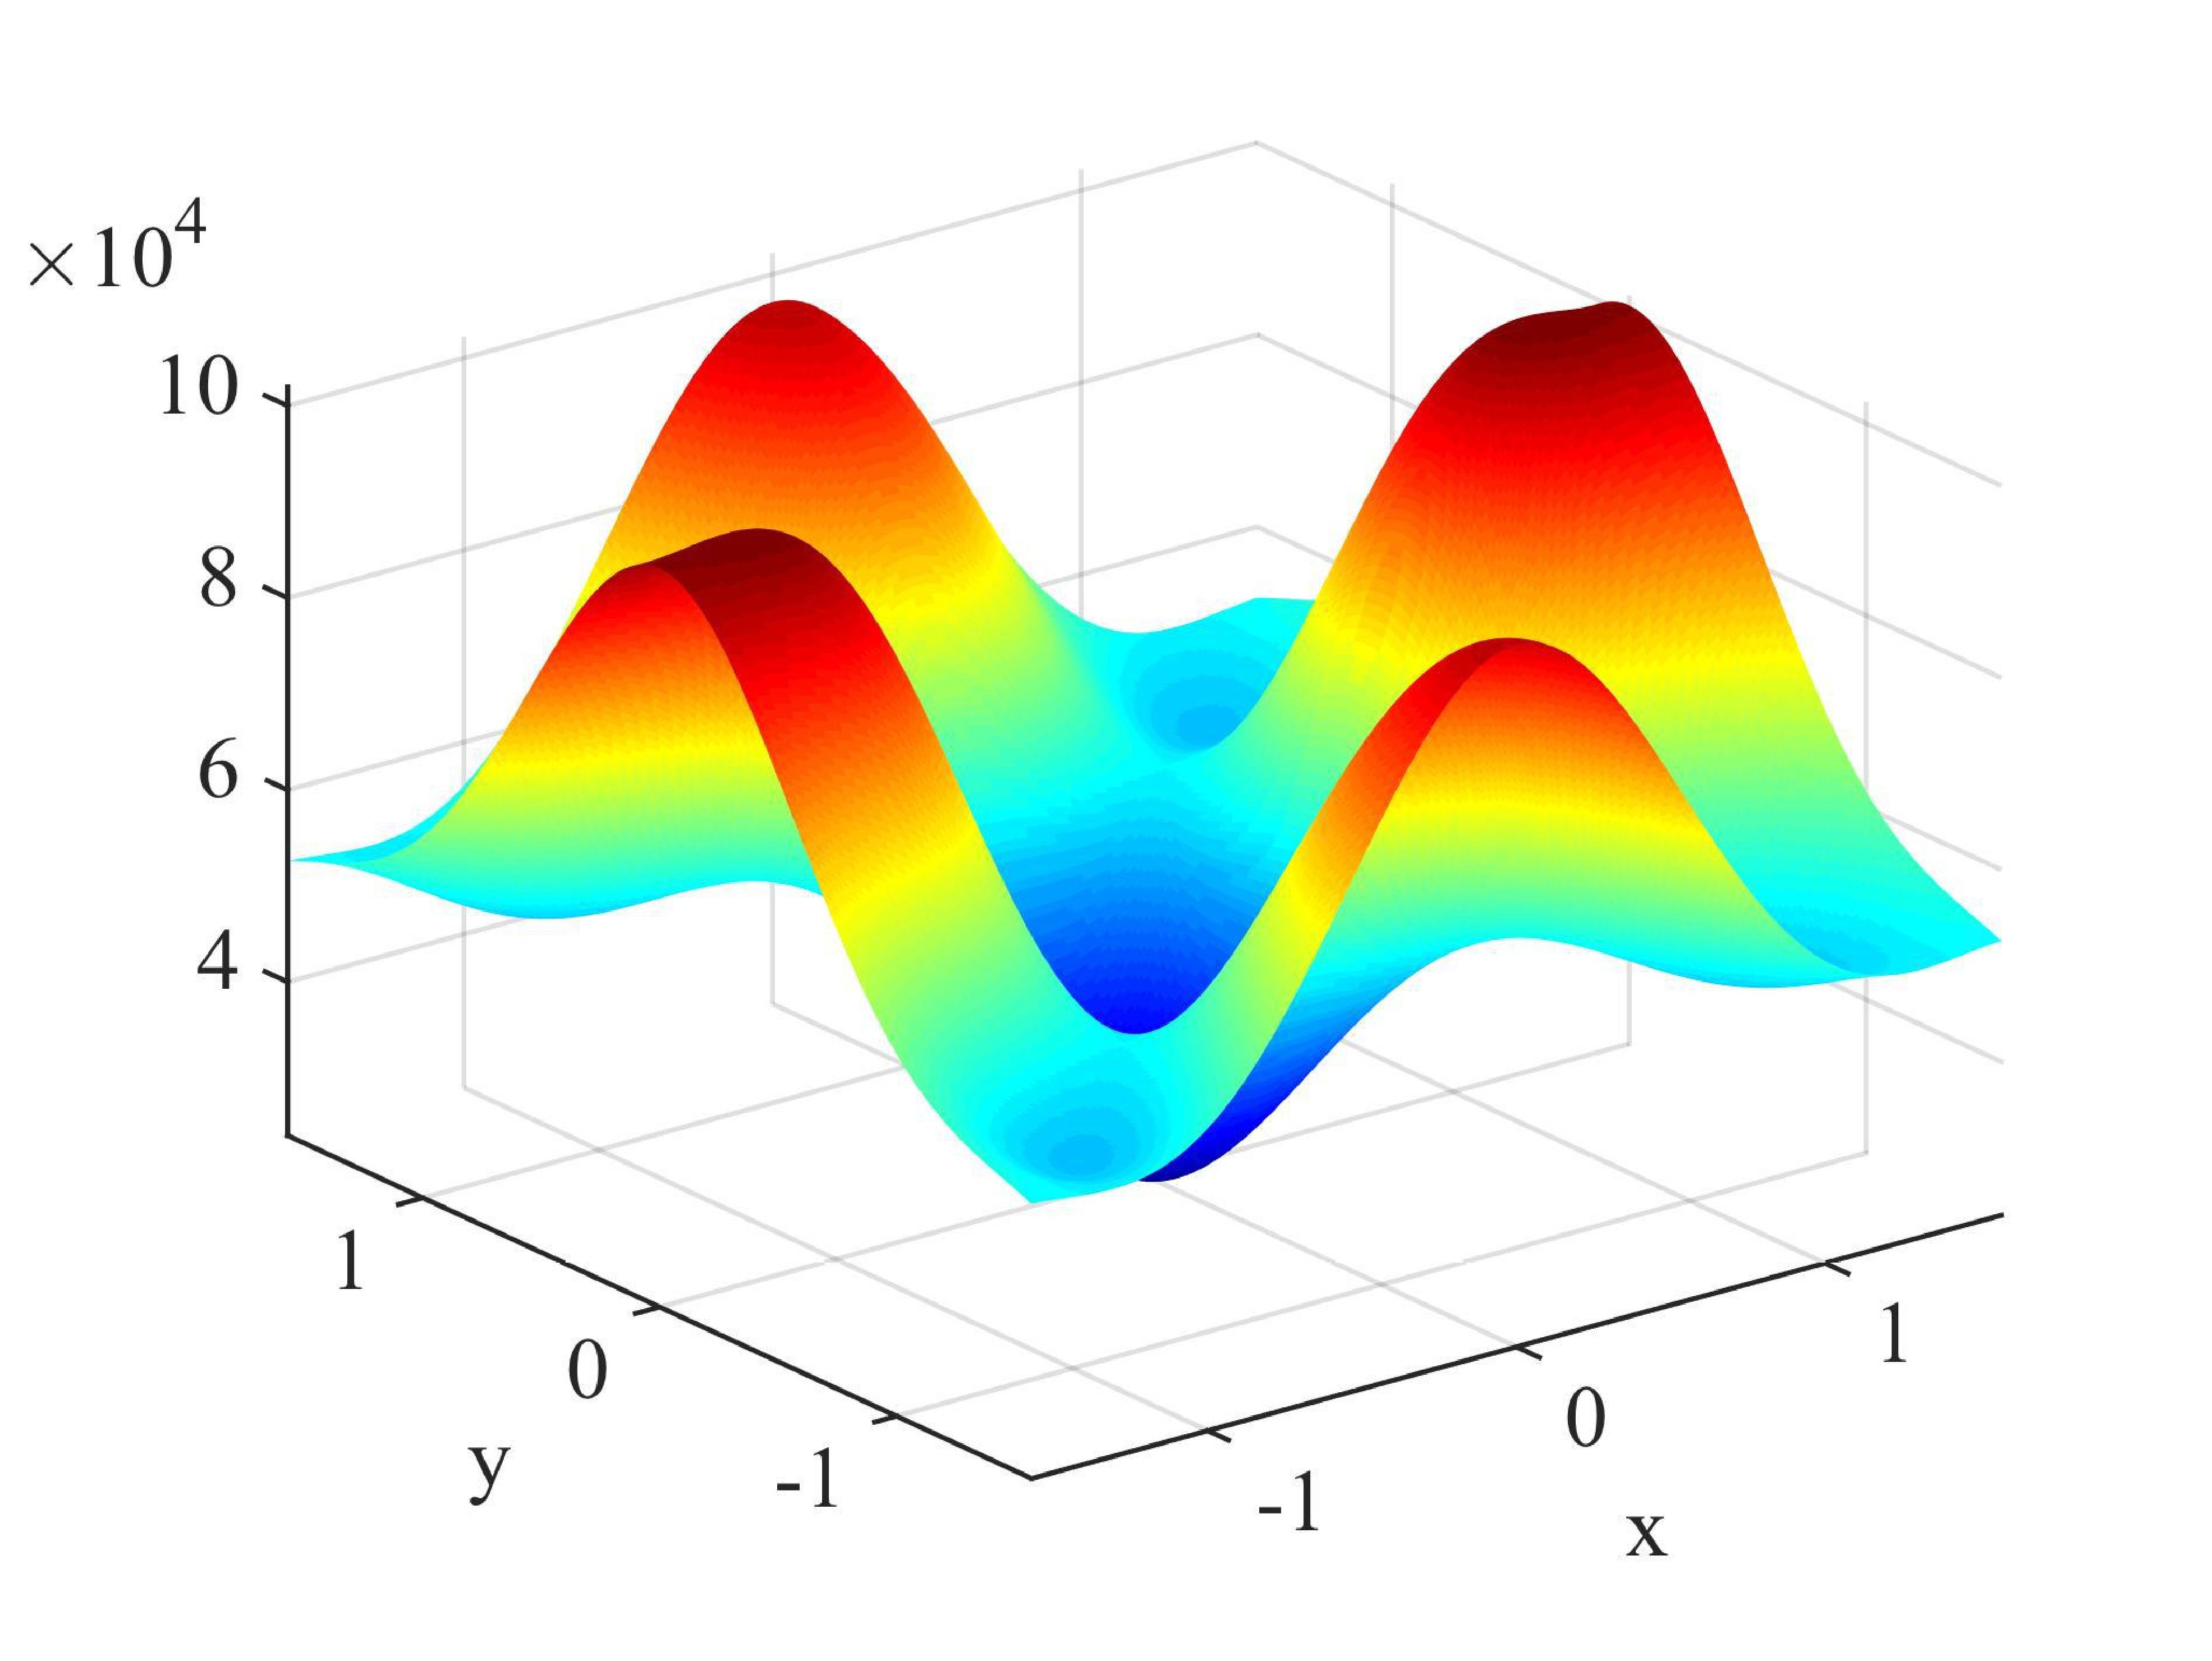
\includegraphics[width=0.45\textwidth]
   {figs/aniso_uniaxial_tangent_detA_F1p1583.pdf}
 } \subfigure[$F_{11}=1.1798$ (bifurcation)]{
   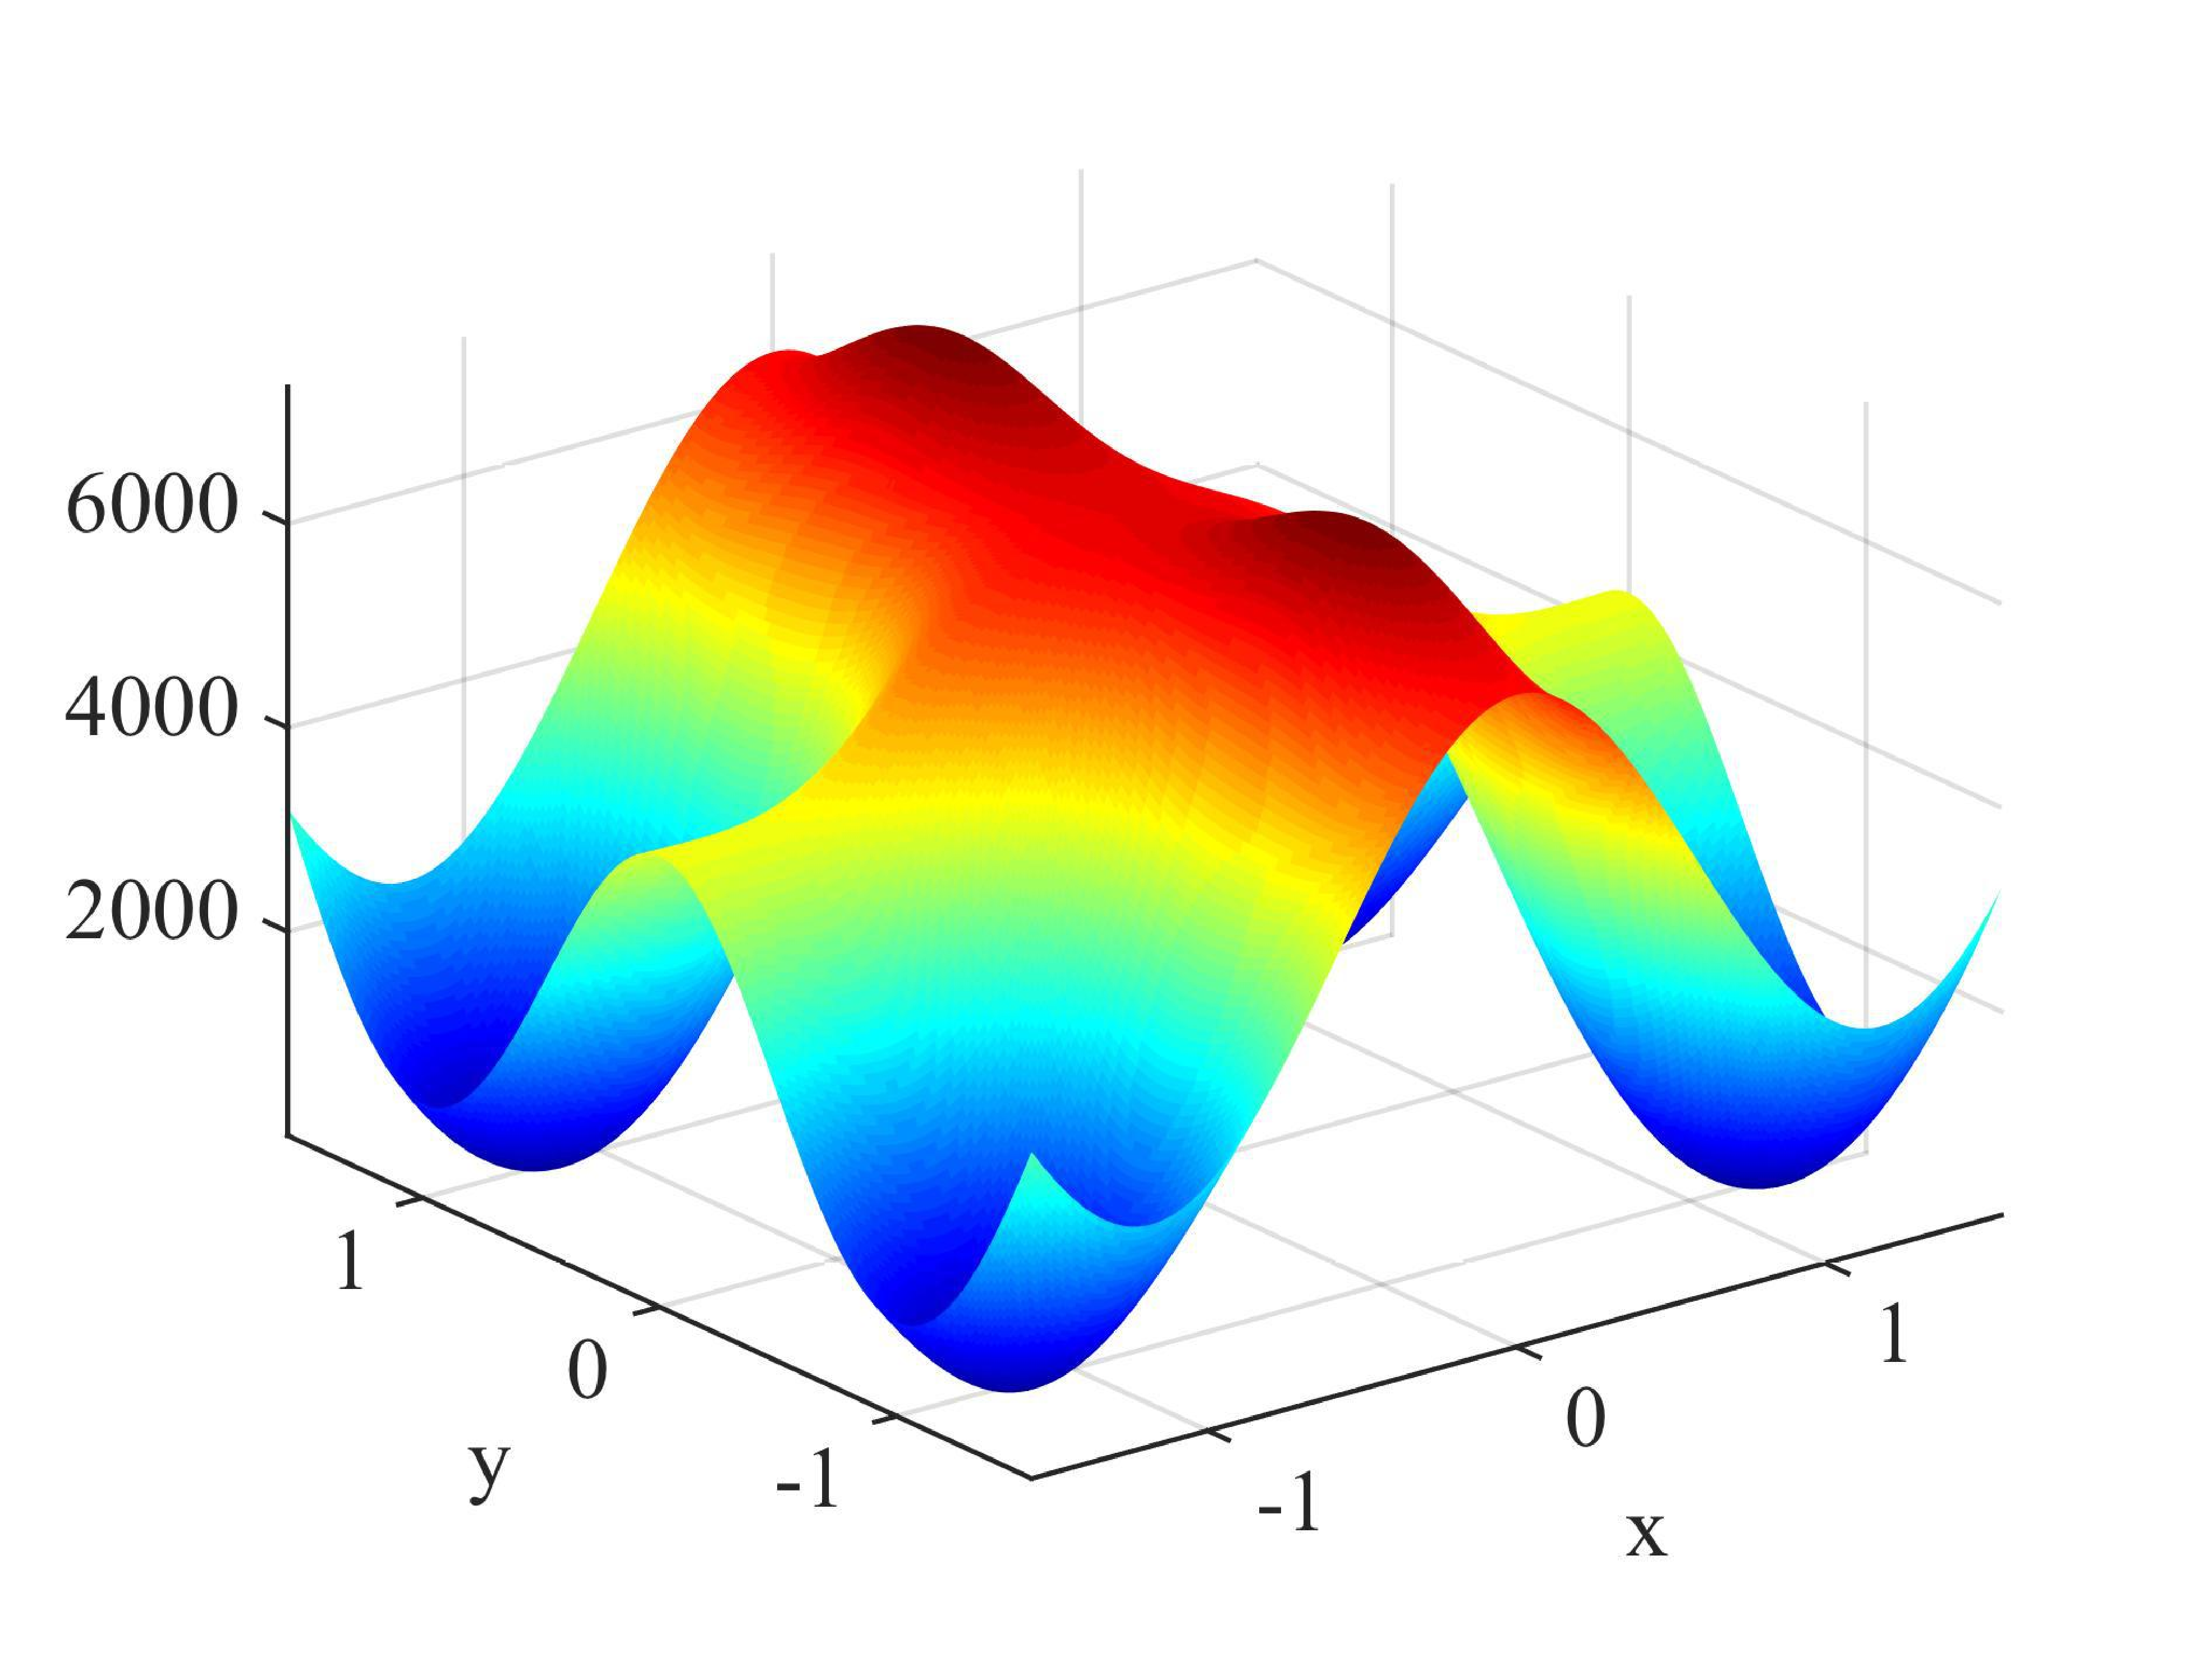
\includegraphics[width=0.45\textwidth]
   {figs/aniso_uniaxial_tangent_detA_F1p1798.pdf}
 }
   \caption{Tangent parametrization: landscapes of $\det~A$ for the
     uniaxial tension test of the finite deformation anisotropic
     model at different axial stretch levels.}
   \label{fig:aniso-tangent-detA}
 \end{figure}

\begin{figure}[!htbp]
   \centering \subfigure[$F_{11}=1.0074$]{
   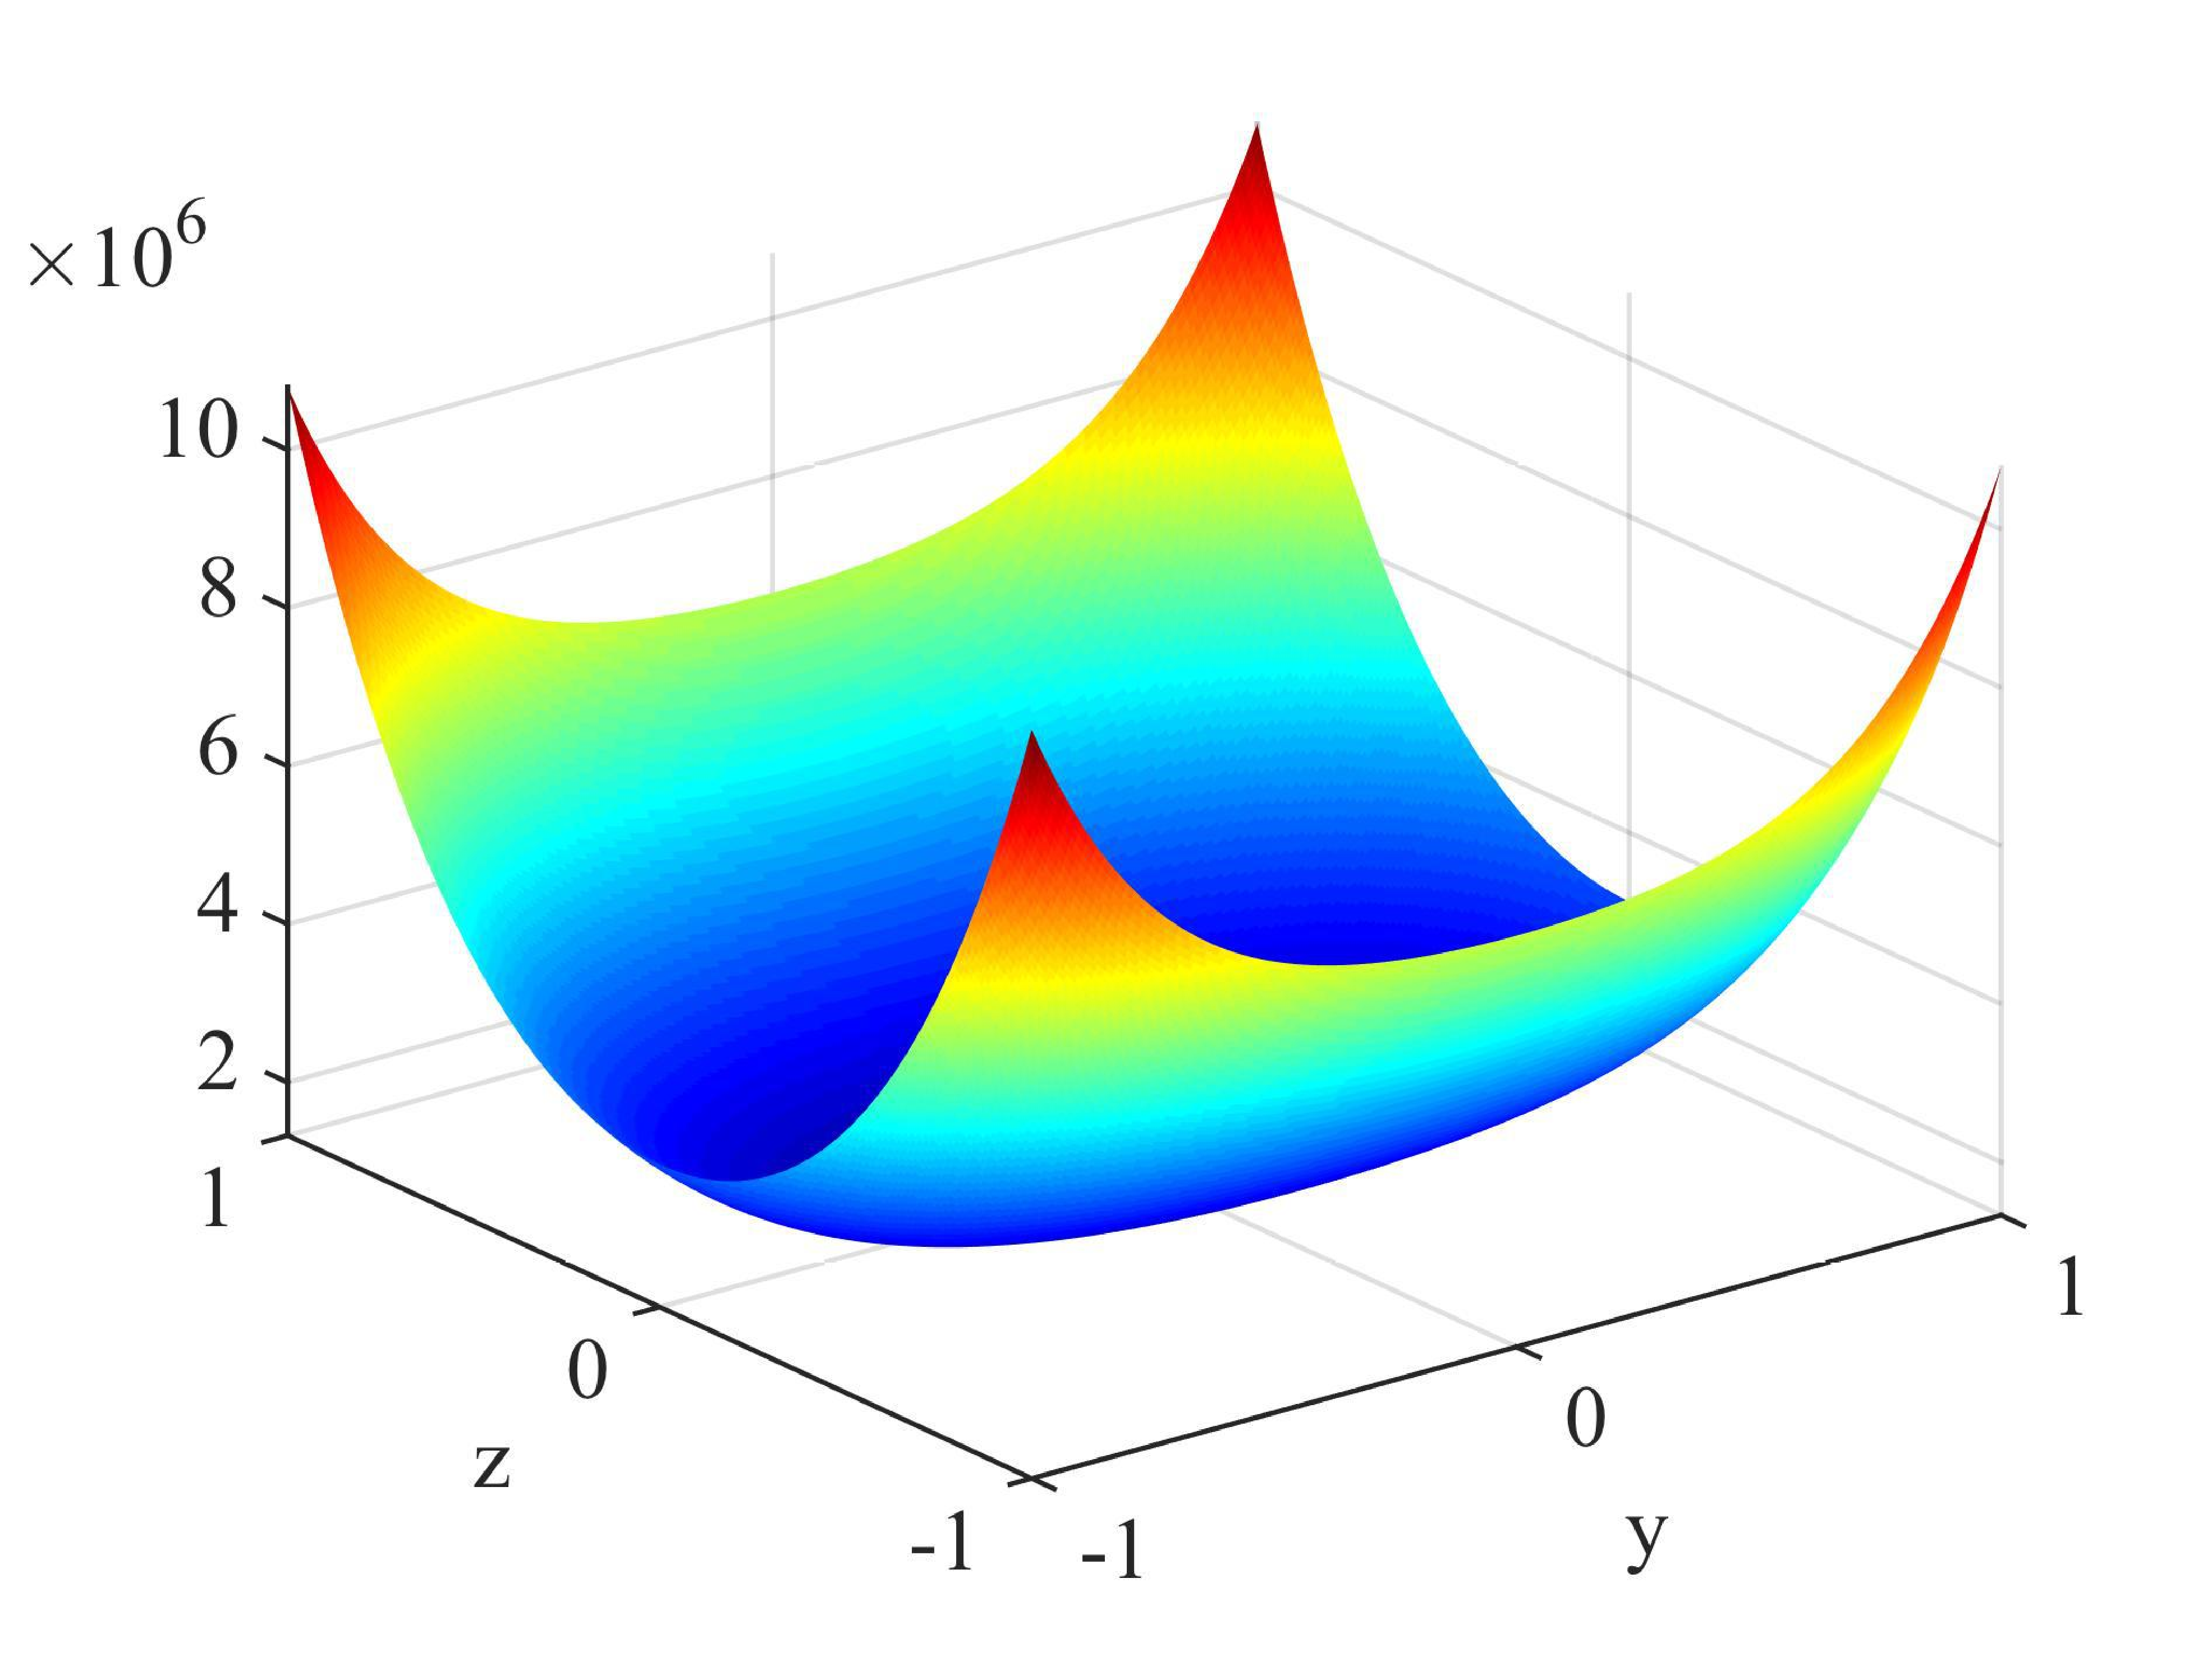
\includegraphics[width=0.45\textwidth]
   {figs/aniso_uniaxial_cartesian_detA_F1p0074.pdf}
 } \subfigure[$F_{11}=1.0762$]{
   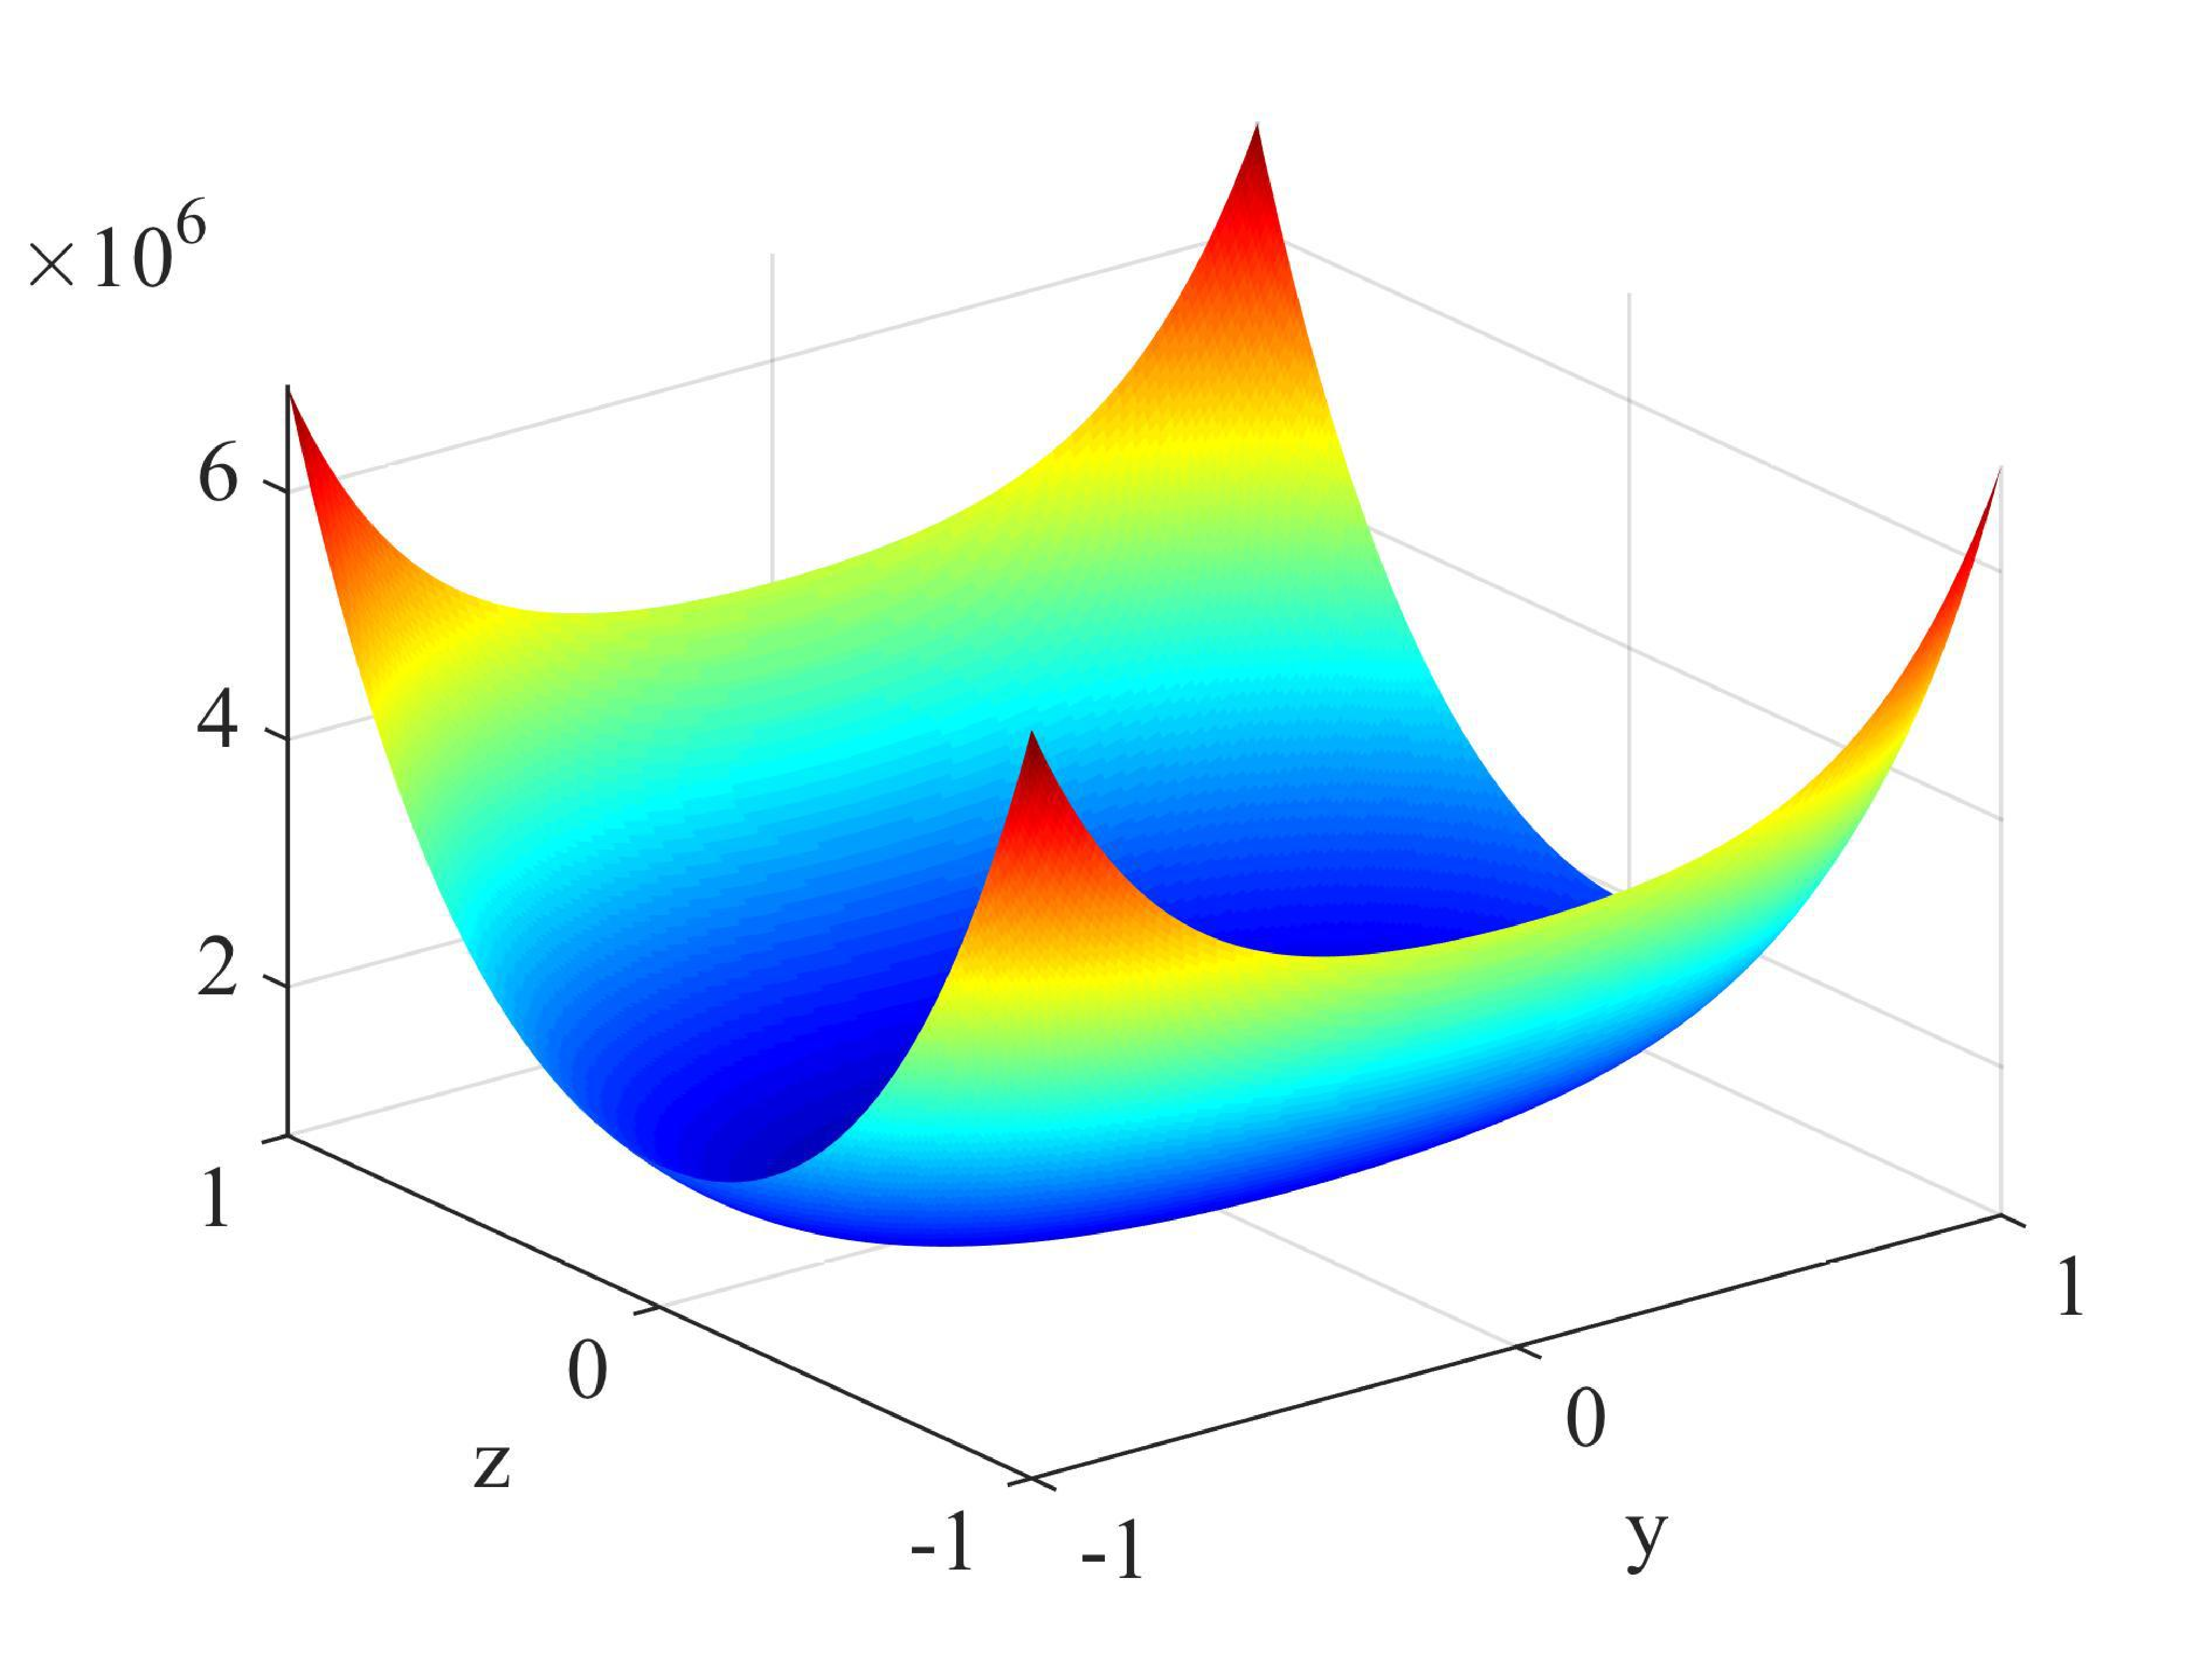
\includegraphics[width=0.45\textwidth]
   {figs/aniso_uniaxial_cartesian_detA_F1p0762.pdf}
 } \subfigure[$F_{11}=1.1583$]{
   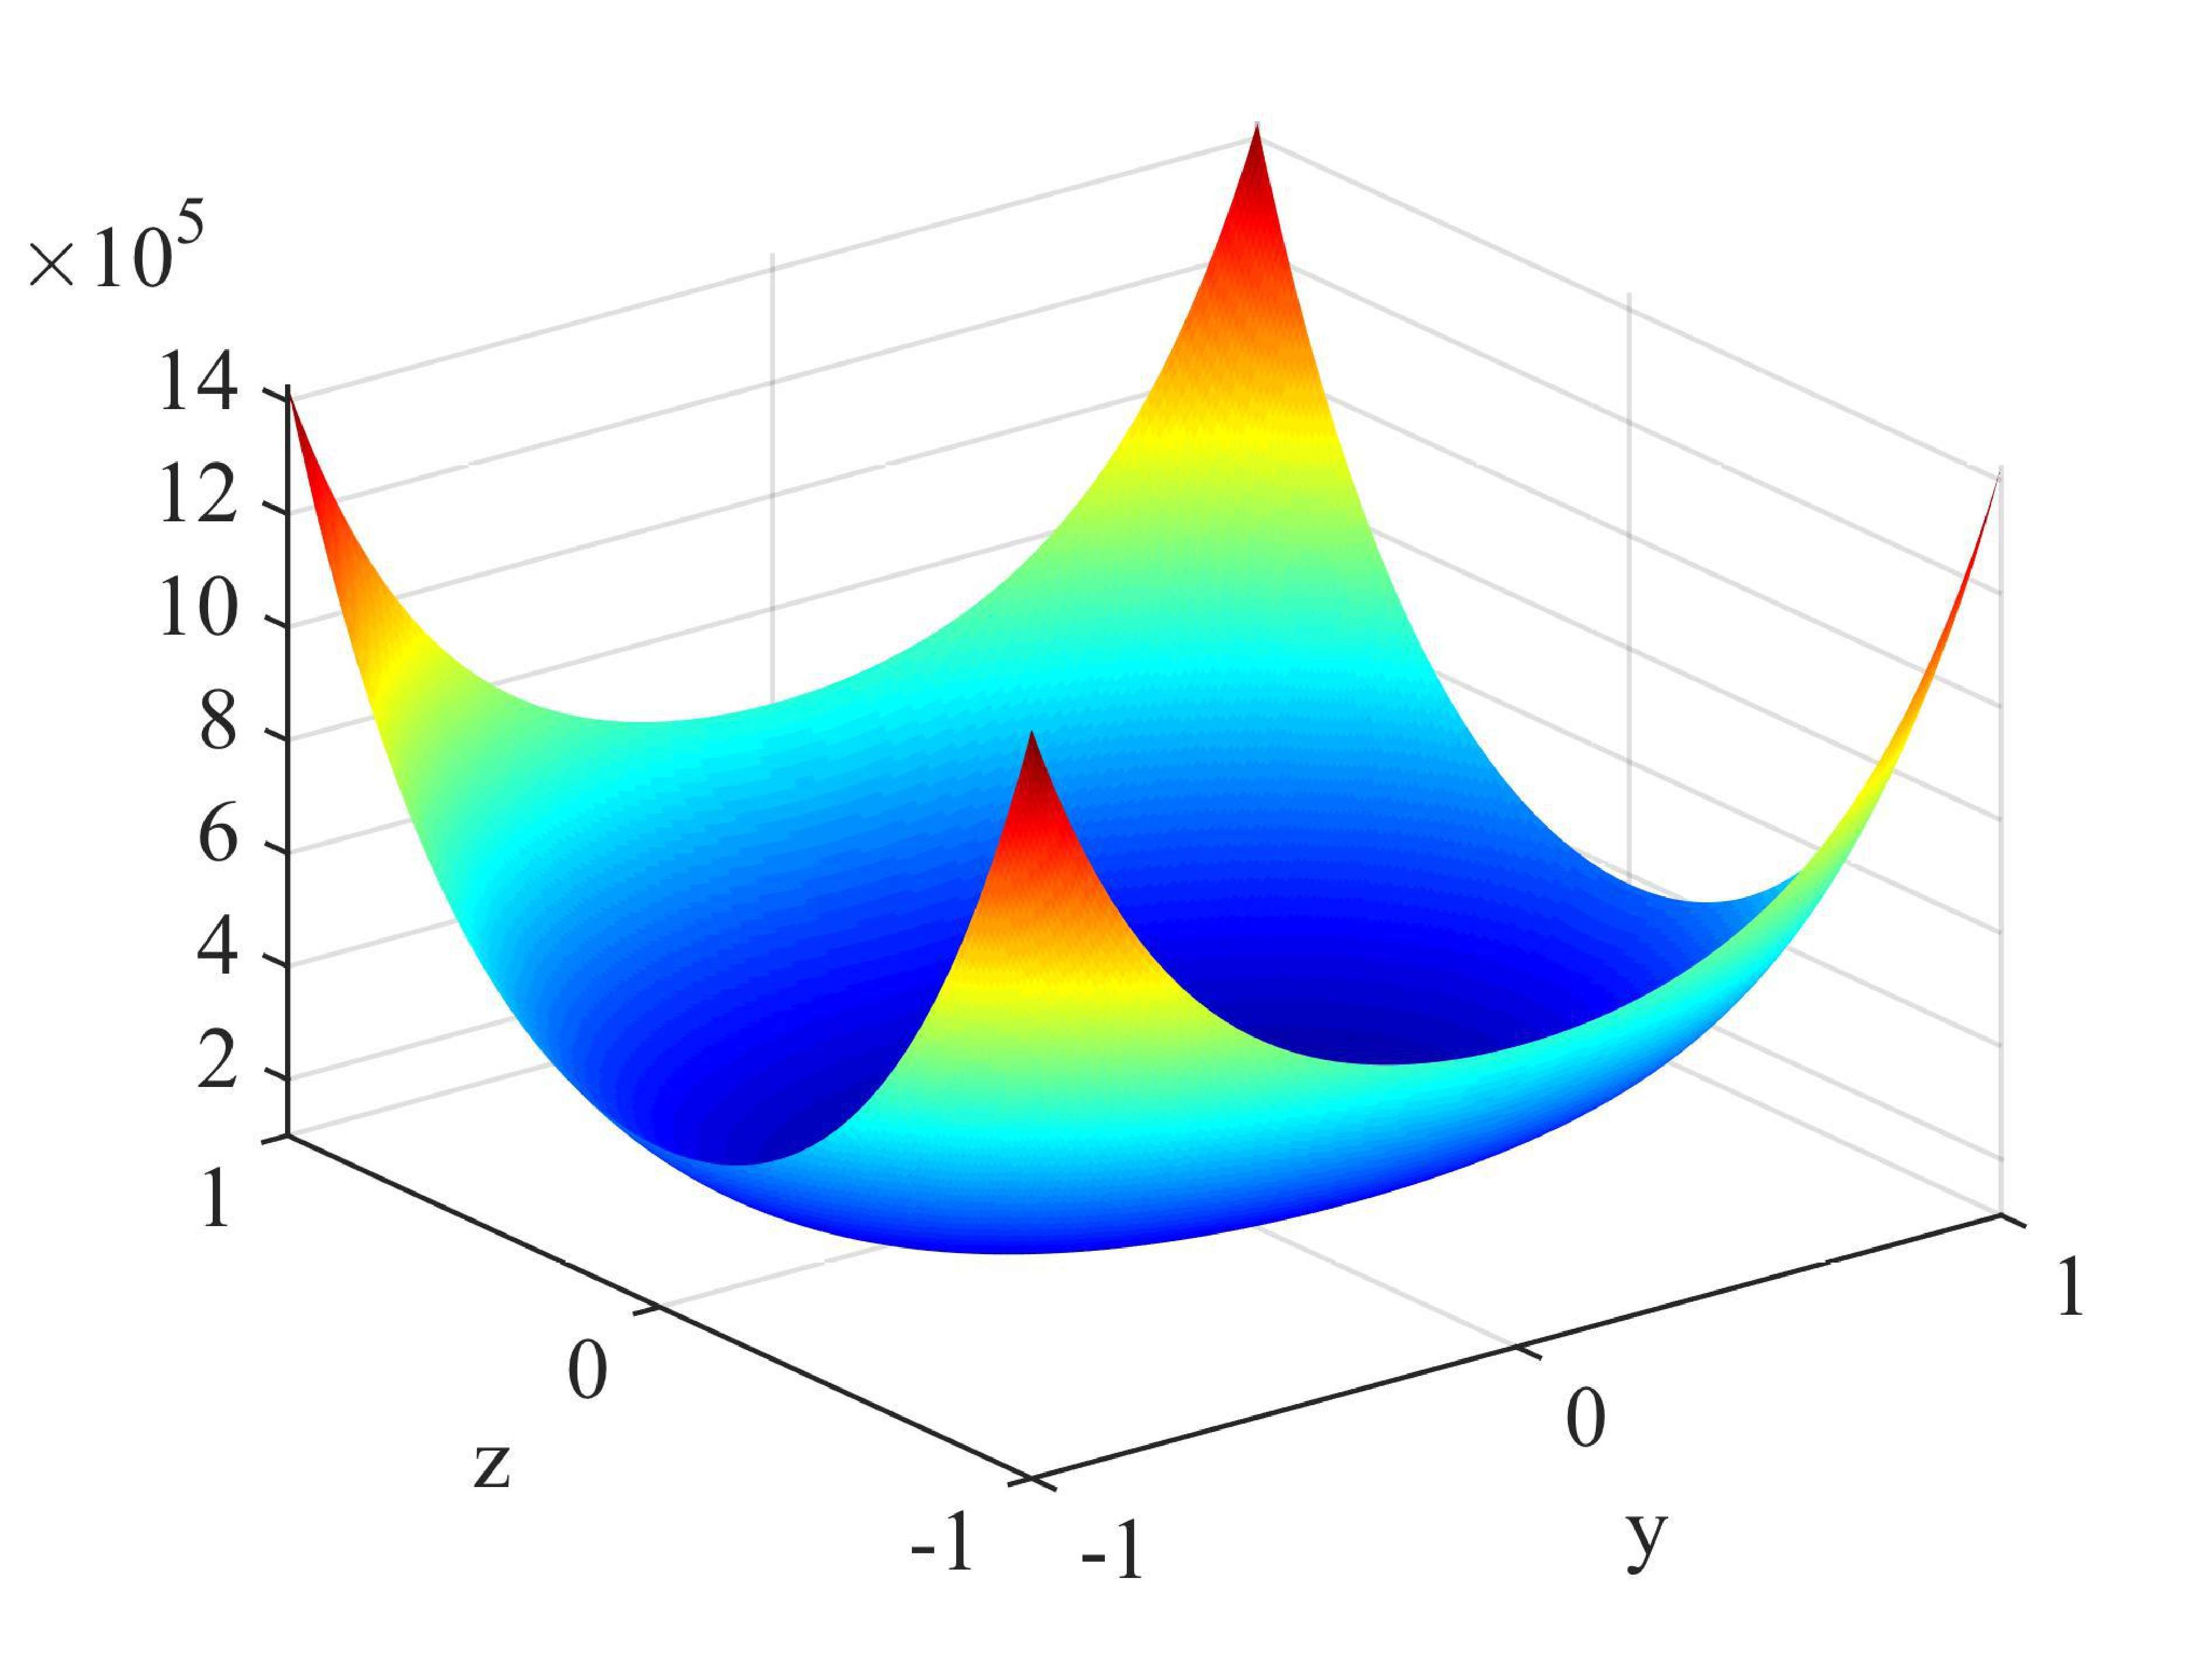
\includegraphics[width=0.45\textwidth]
   {figs/aniso_uniaxial_cartesian_detA_F1p1583.pdf}
 } \subfigure[$F_{11}=1.1798$ (bifurcation)]{
   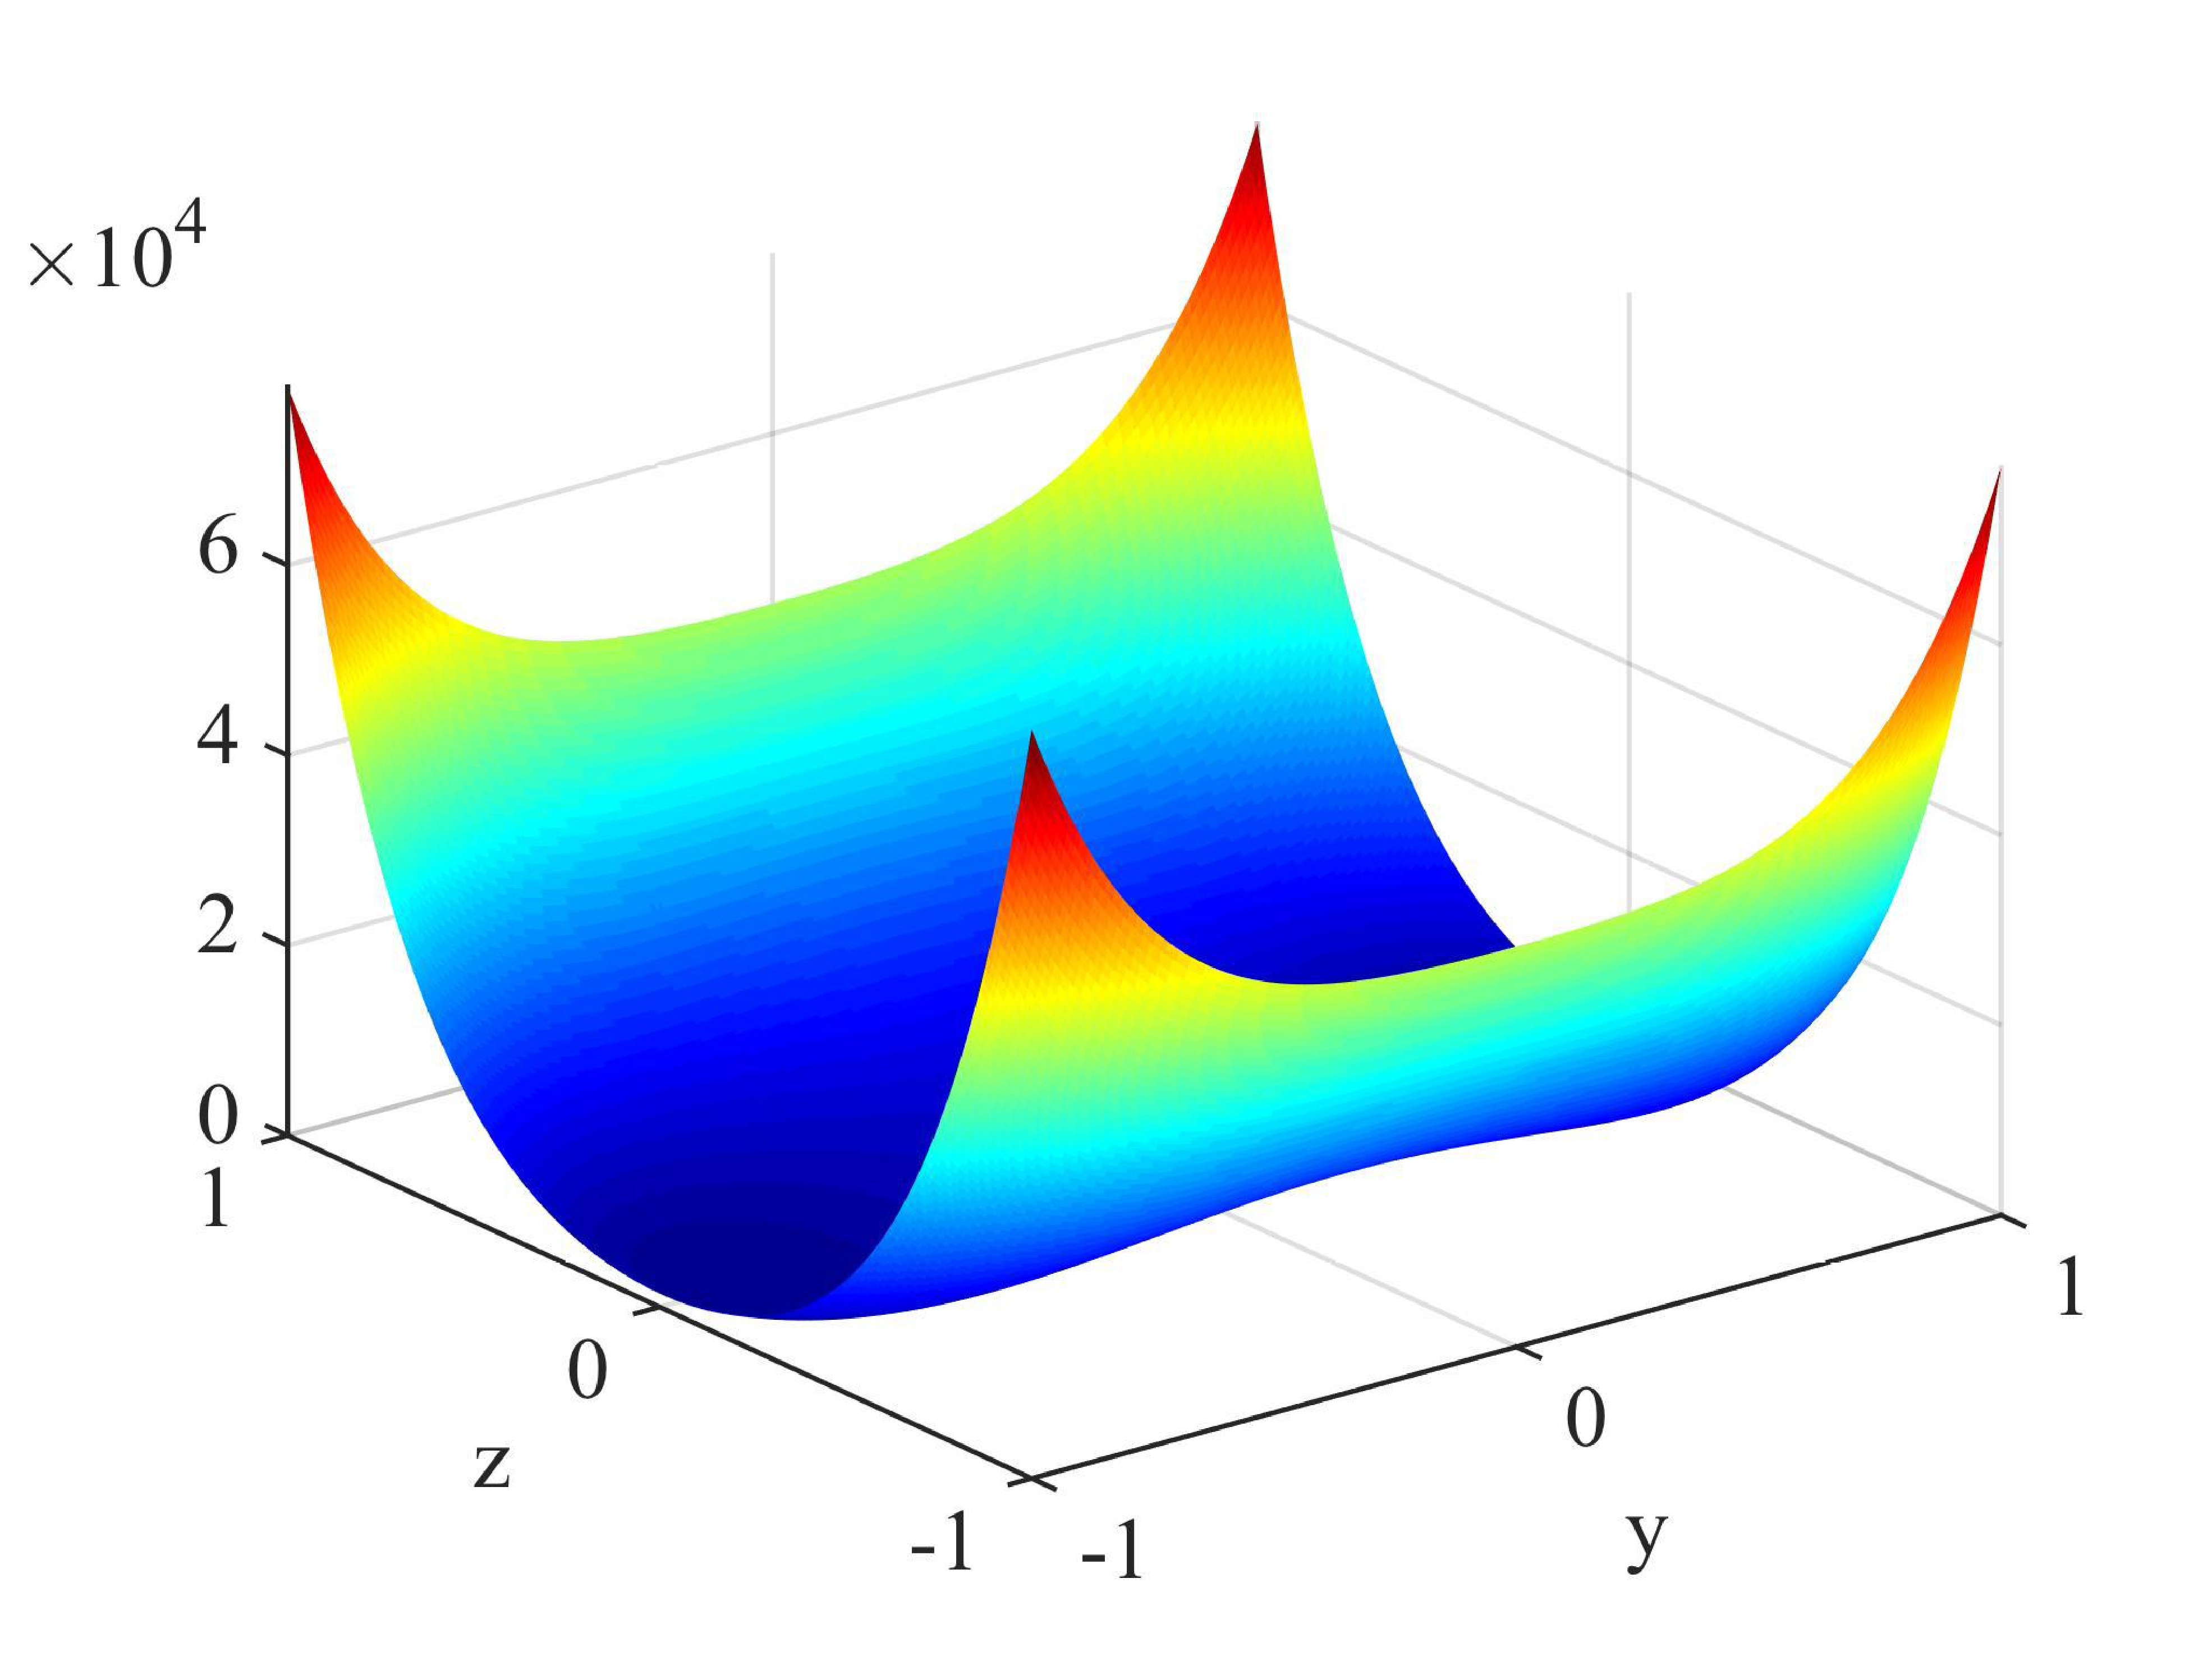
\includegraphics[width=0.45\textwidth]
   {figs/aniso_uniaxial_cartesian_detA_F1p1798.pdf}
 }
   \caption{Cartesian parametrization: landscapes of $\det~A$ for the
     uniaxial tension test of the finite deformation anisotropic
     model at different axial stretch levels.}
   \label{fig:aniso-cartesian-detA}
 \end{figure}

\begin{figure}[!htbp]
   \centering \subfigure[Spherical]{
   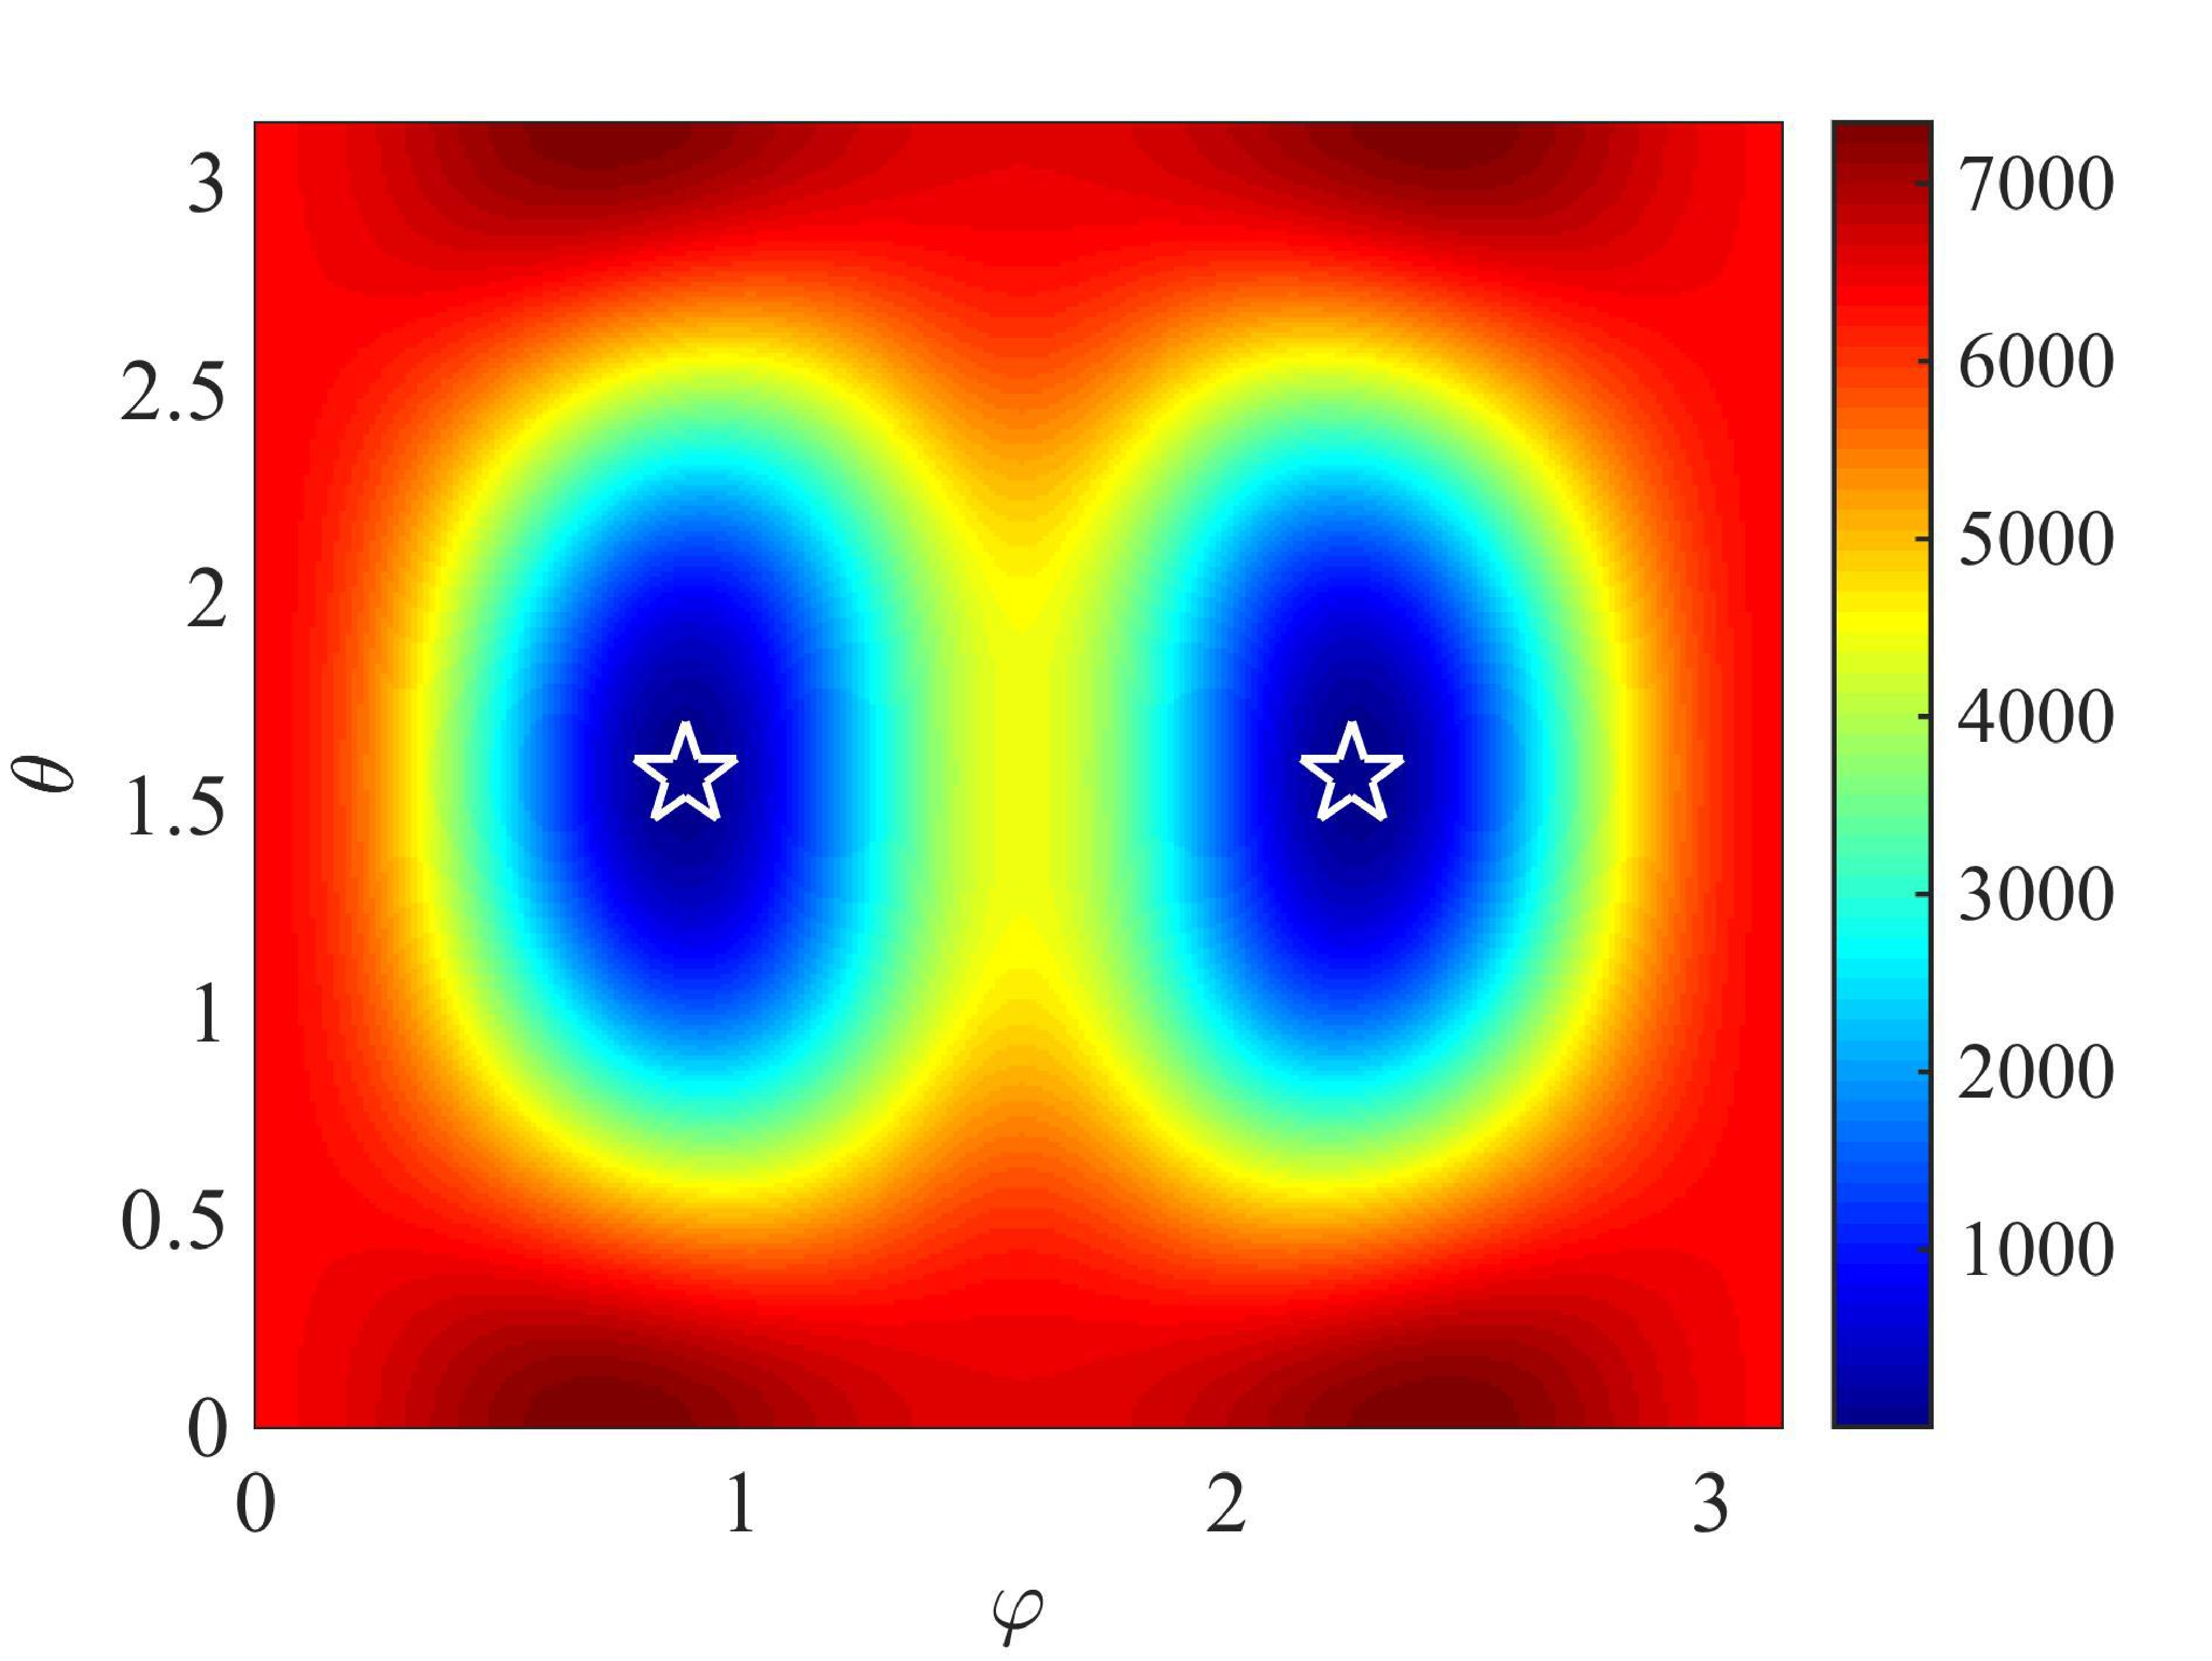
\includegraphics[width=0.45\textwidth]
   {figs/aniso_uniaxial_spherical_detAXplane.pdf}
 } \subfigure[Cartesian]{
   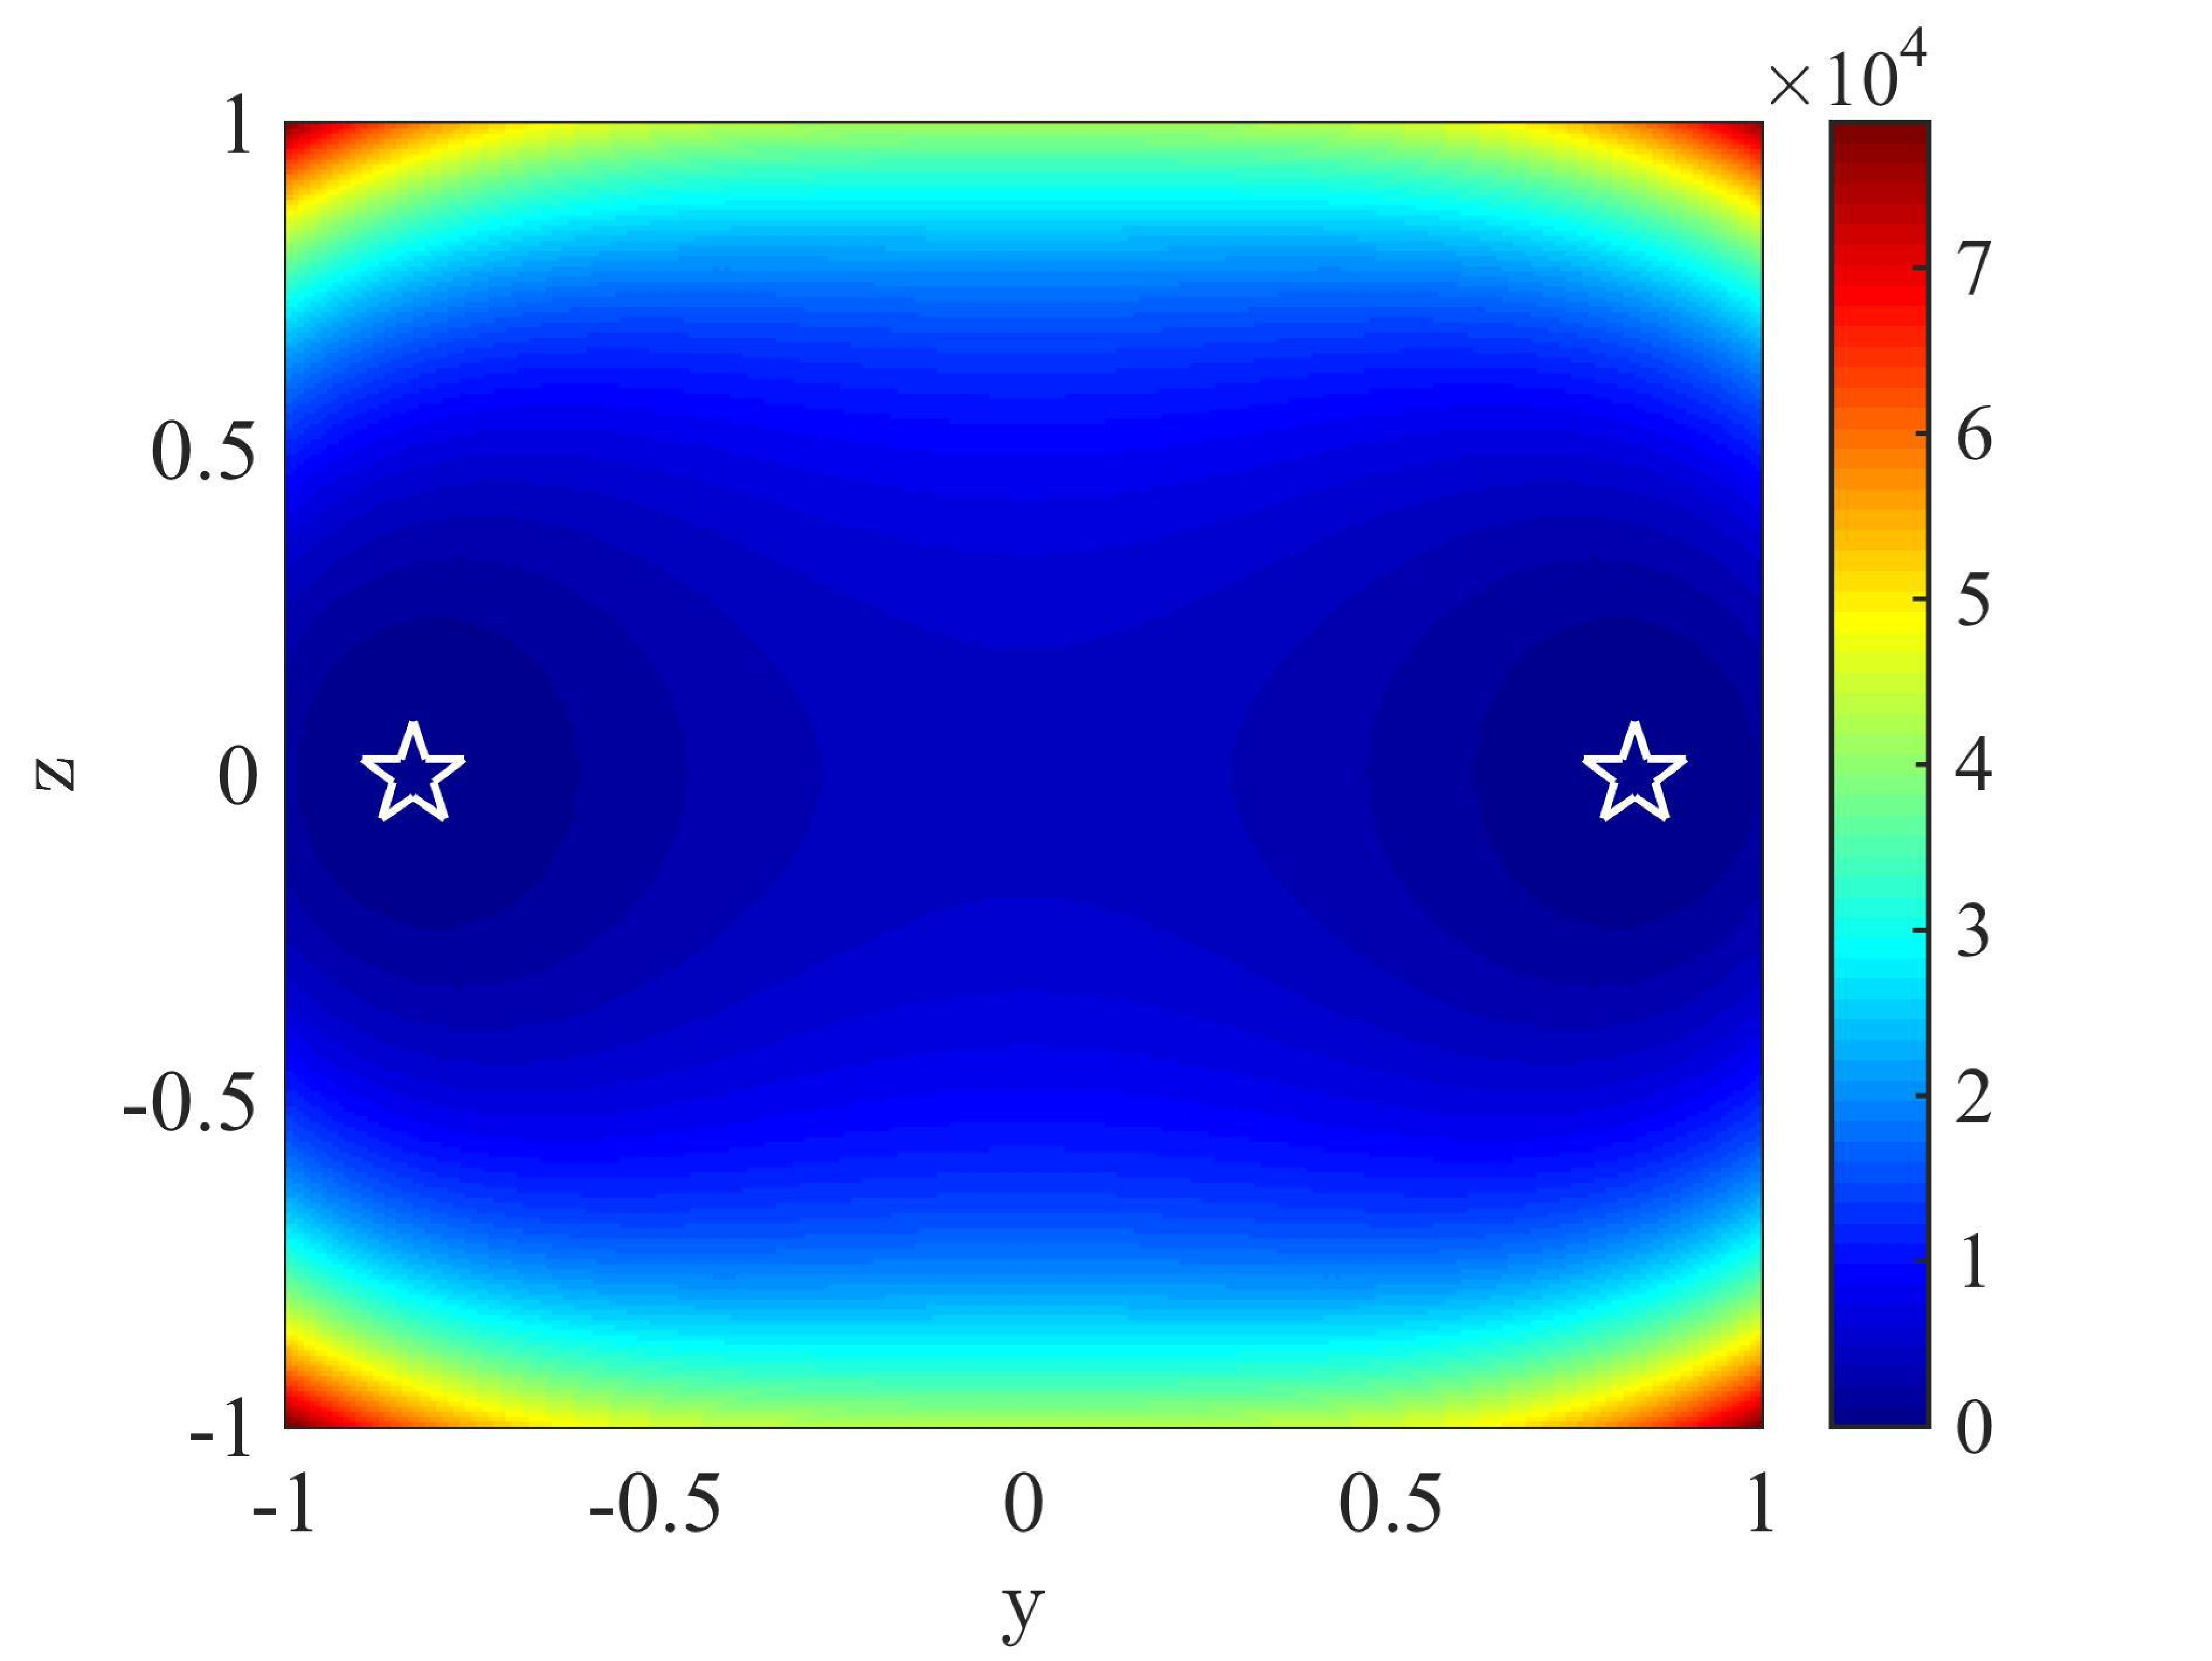
\includegraphics[width=0.45\textwidth]
   {figs/aniso_uniaxial_cartesian_detAXplane.pdf}
 } \subfigure[Stereographic]{
   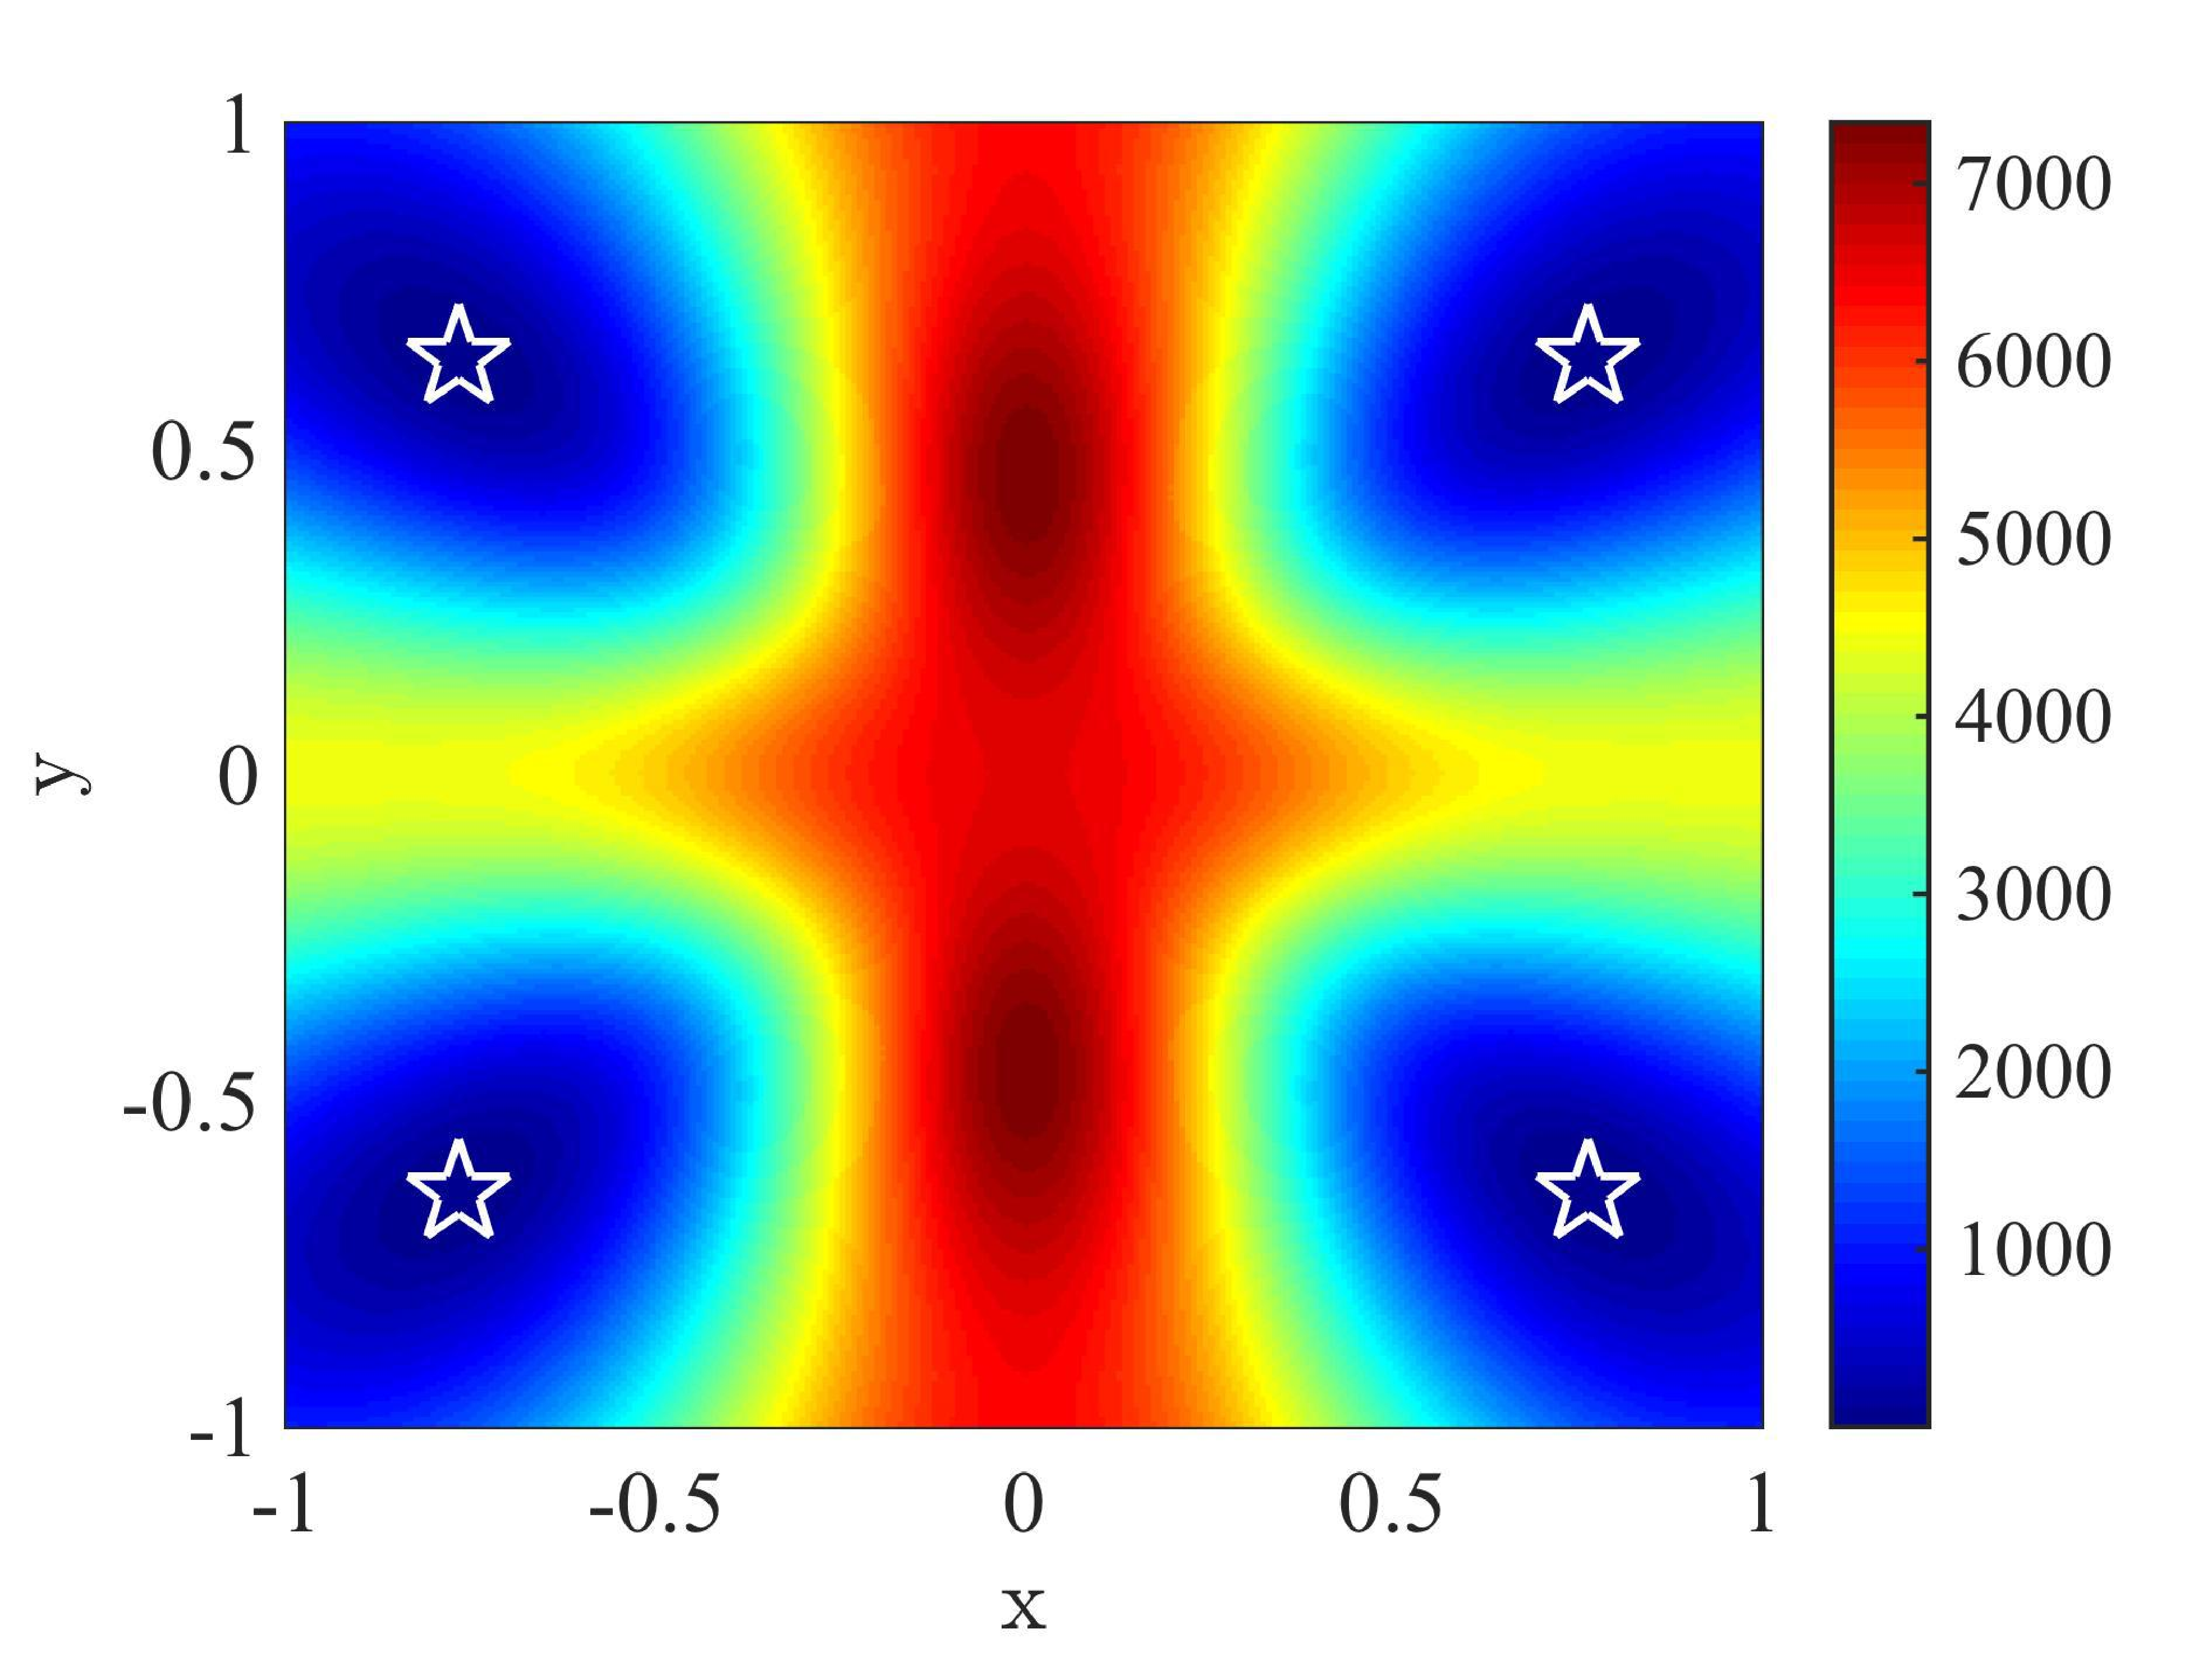
\includegraphics[width=0.45\textwidth]
   {figs/aniso_uniaxial_stereographic_detAXplane.pdf}
 } \subfigure[Tangent]{
   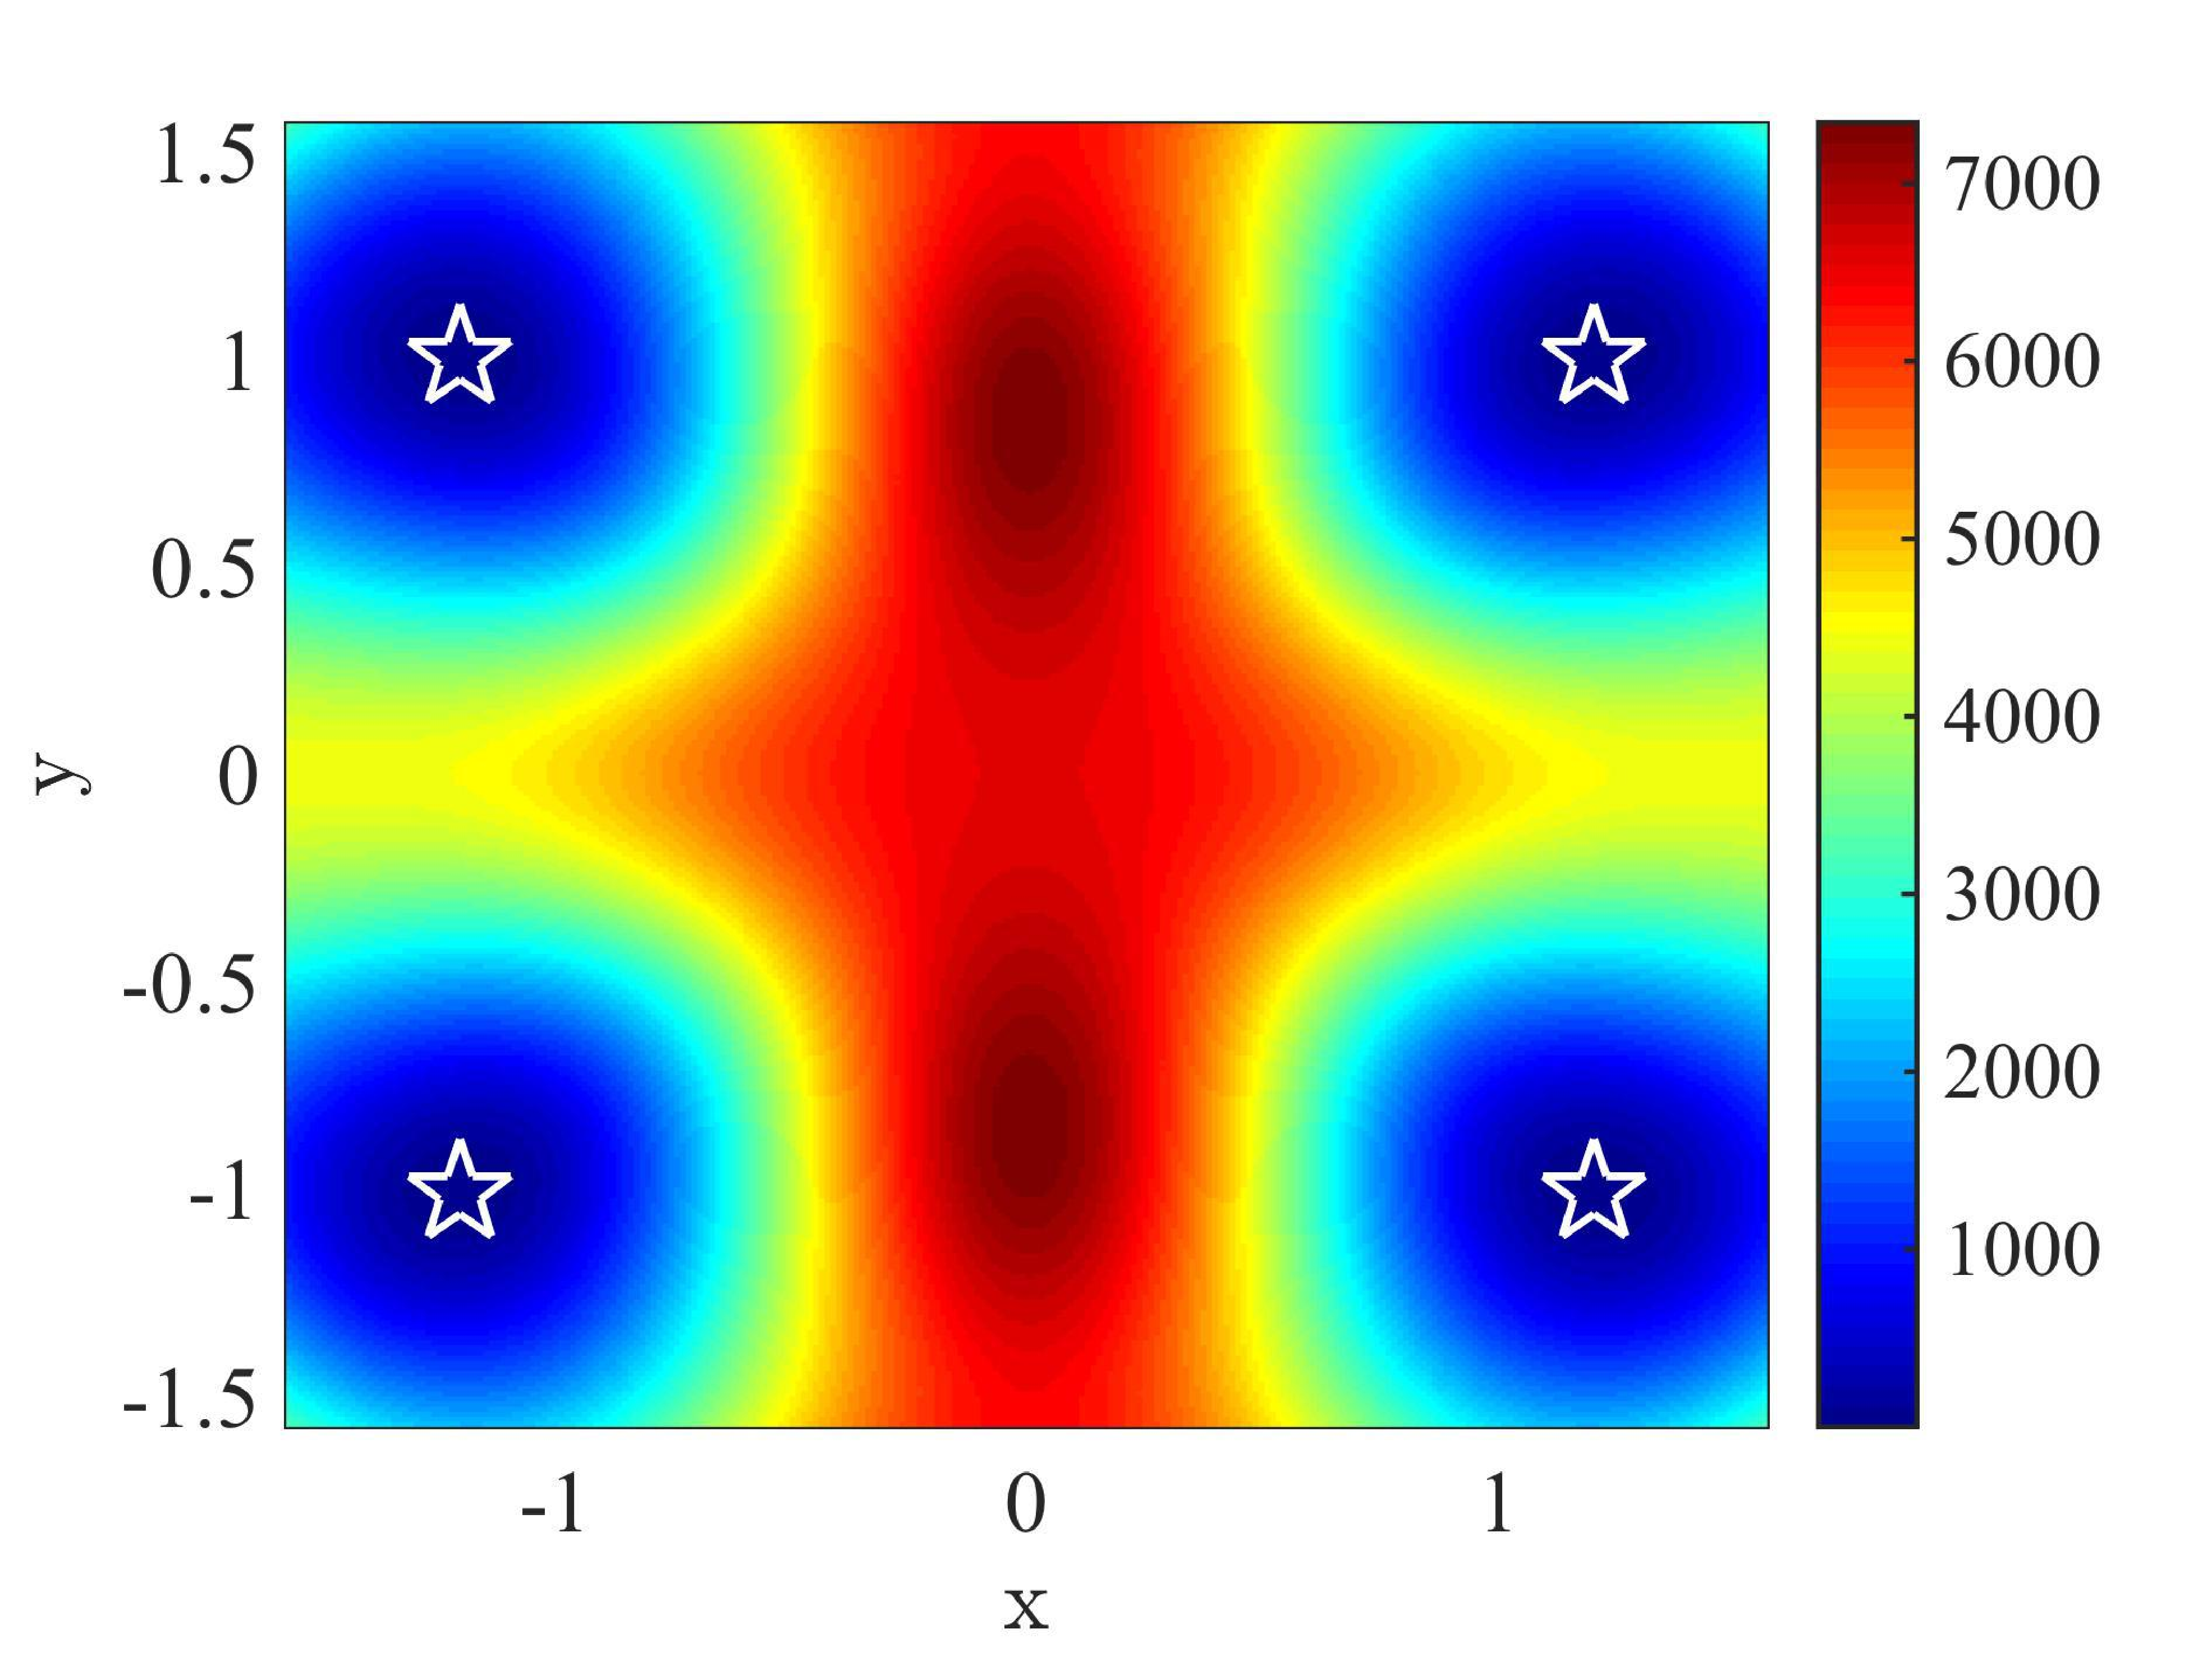
\includegraphics[width=0.45\textwidth]
   {figs/aniso_uniaxial_tangent_detAXplane.pdf}
 }
   \caption{Plane views of the landscapes of the determinant of the
     acoustic tensor at bifurcation for the uniaxial tension on the
     finite deformation anisotropic model. The white stars indicate
     global minima.}
   \label{fig:aniso-uniaxial-detAXplane}
 \end{figure}
 
As can be seen from \fref{fig:aniso-cartesian-detA}, the Cartesian
parametrization again results in a simple, bowl-shaped landscape of
the determinant function consistently throughout the loading process,
which is in contrast to the more complex landscapes of the spherical
(\fref{fig:aniso-spherical-detA}), stereographic
(\fref{fig:aniso-stereographic-detA}) and tangent
(\fref{fig:aniso-tangent-detA}) parametrizations.

As in the case of the small deformation model example in Section
\ref{subsec:isotropic}, the robustness of the different
parametrizations on the detection of material bifurcation is analyzed
by randomly generating a single initial point for the Newton iterative
scheme and eliminating the initial sampling. A total of 1000 random
initial guesses are generated for each parametrization. The success
rate and computation time are recorded and summarized in
Table~\ref{tab:aniso-axial-random-para}. The results are consistent
with the small deformation model example, \ie, the Cartesian
parametrization is most robust and computationally efficient of all
the ones tested.

\begin{table}[!htbp]
 \begin{center}
  \begin{tabular}{l | c c c c c}
    \toprule
    & Spherical & Stereographic & Projective & Tangent & Cartesian     \\
    \midrule
    Success rate ($\%$)      & 13.4 & 32.3  & 71.5  & 32.3  &  74.4   \\
    Average iteration count    & 4.37 & 4.91 & 8.04  & 4.57 & 6.93   \\
    Average run time (${\mu}s$)  & 270  & 274  & 483  & 245  & 267   \\
    \bottomrule
  \end{tabular}
  \caption{Anisotropic finite deformation model: success rate and
    computation time of the Newton iterative scheme with a single random
    initial guess. A total of 1000 random trials are performed for
    each parametrization.}
    \label{tab:aniso-axial-random-para}
 \end{center}
\end{table}

A visualization of the robustness of each parametrization with 1000
random initial guesses is shown in
\fref{fig:aniso-uniaxial-robust}. If the initial guess leads to a
success detection of bifurcation and its directions, the point is
marked as a solid circle ($\bullet$). Otherwise, it is marked as a
cross ($\times$).

\begin{figure}[!htbp]
   \centering \subfigure[Spherical]{
   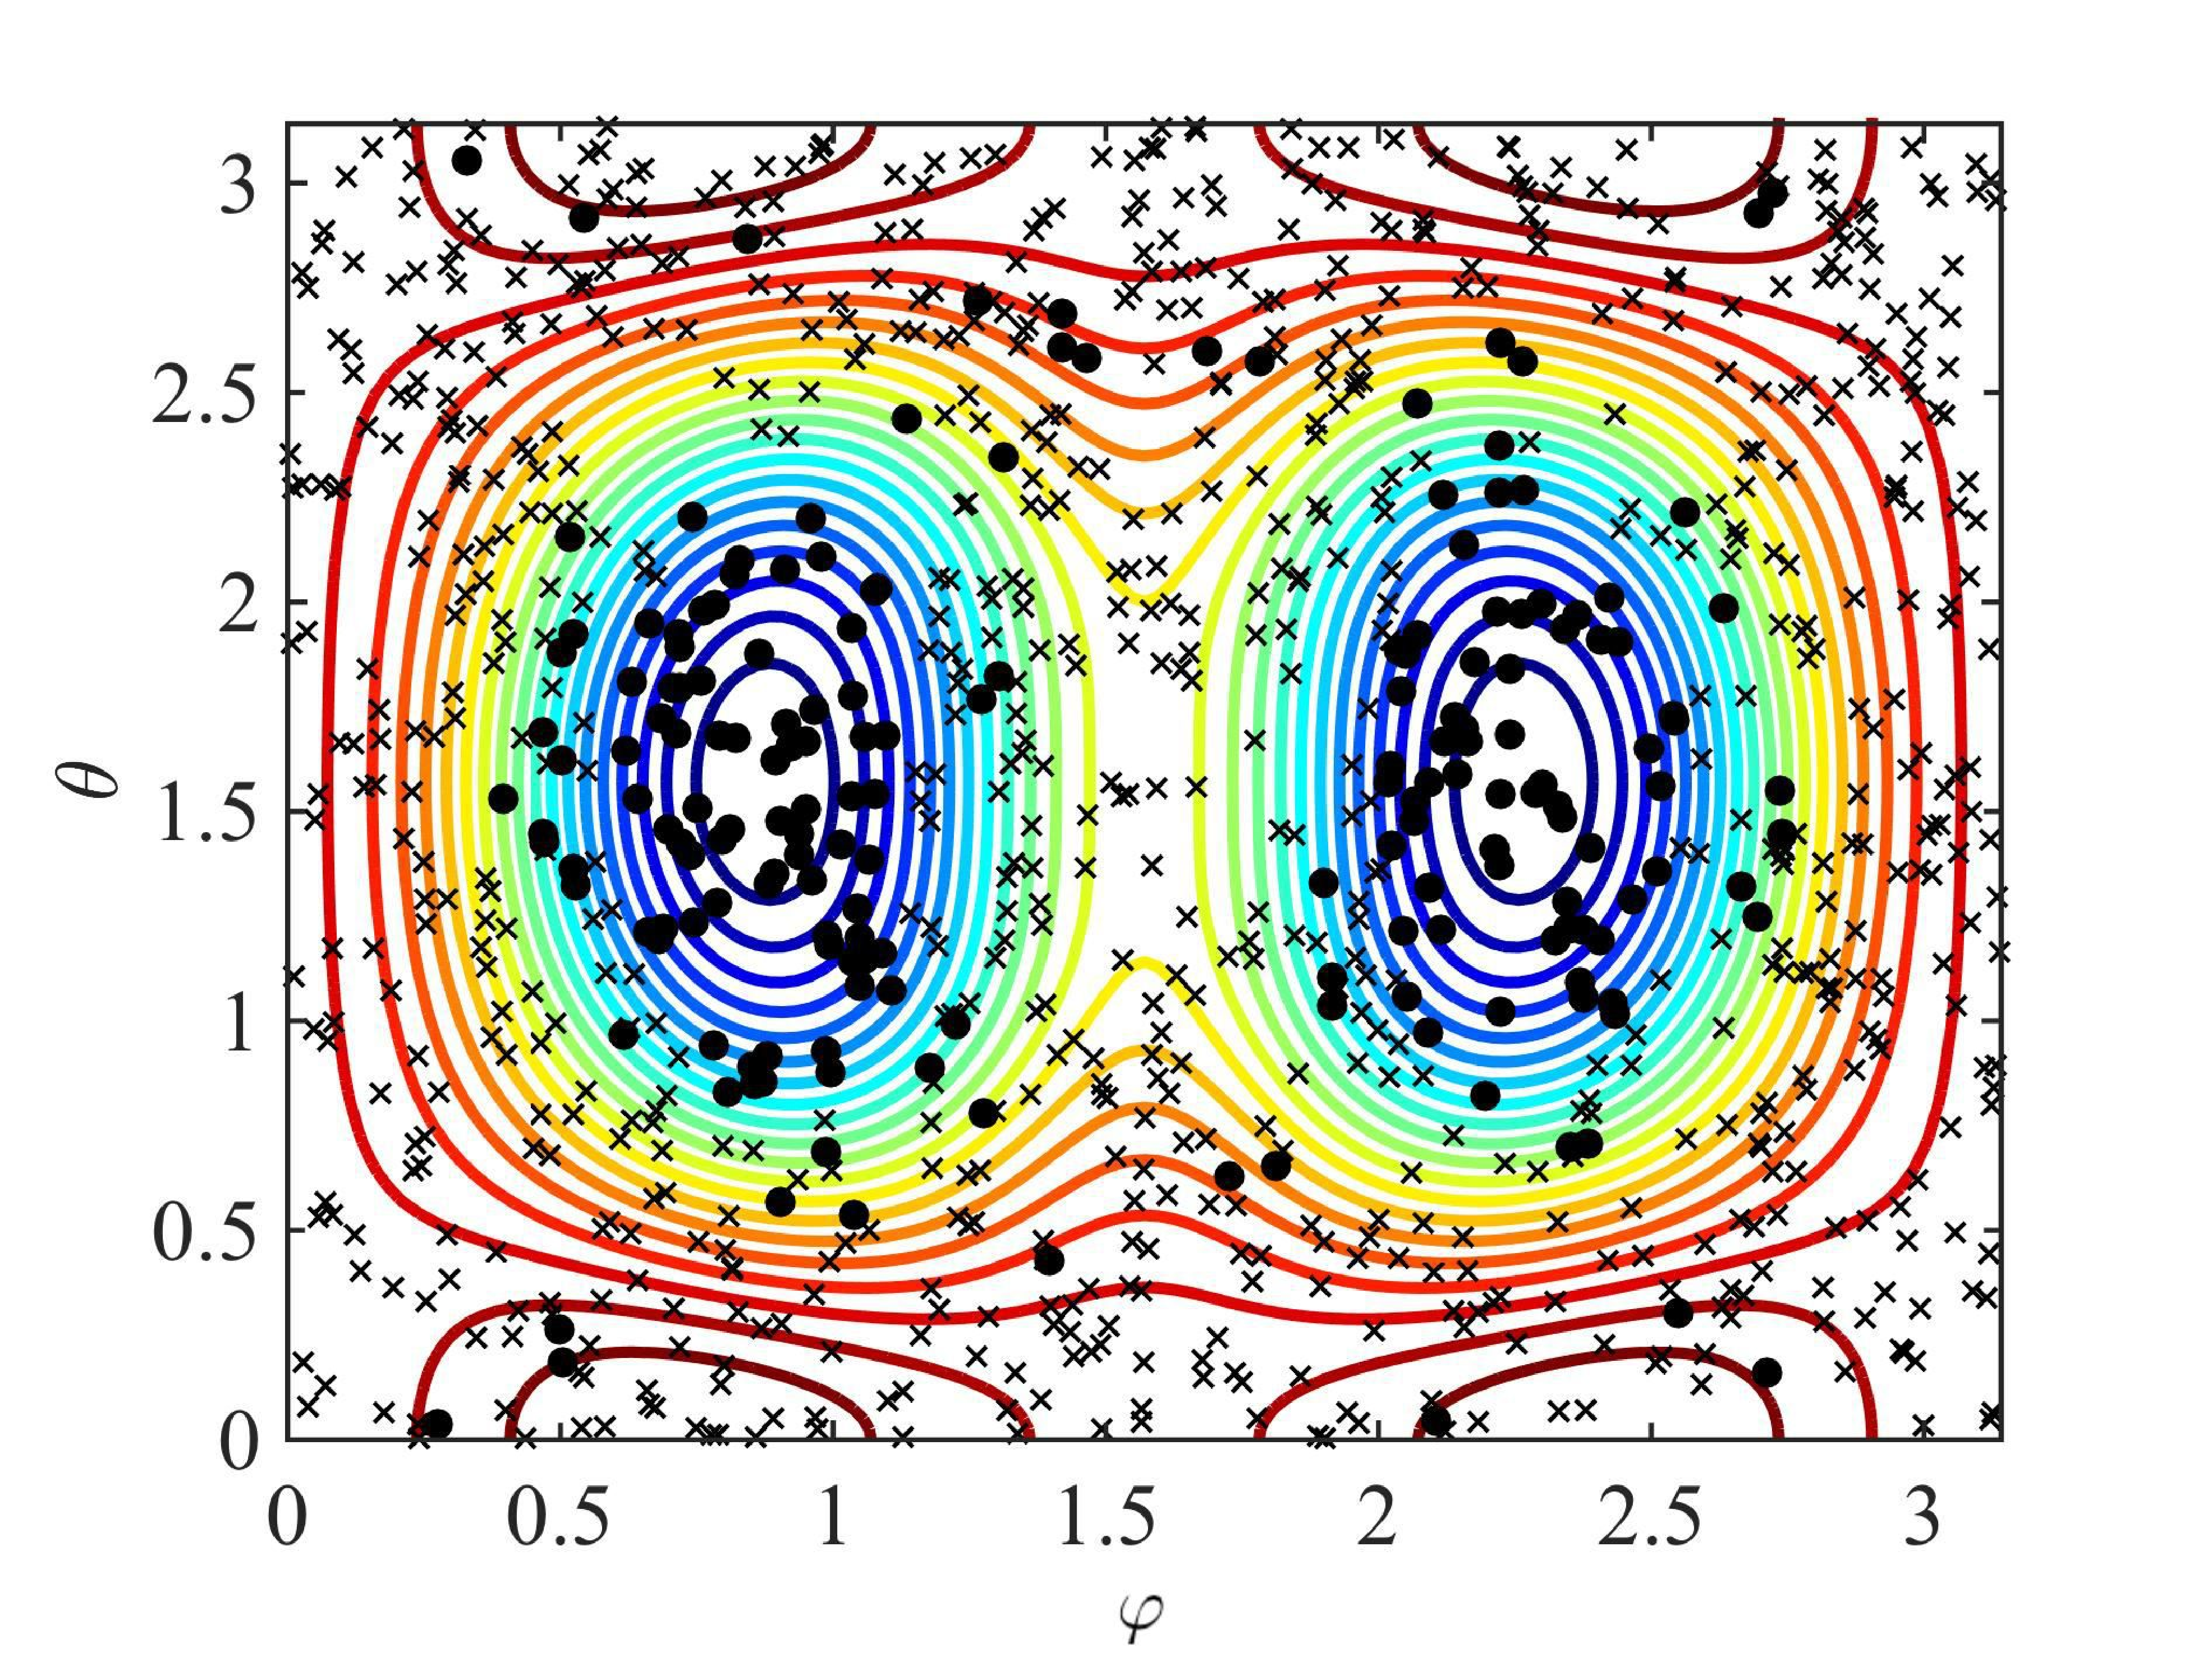
\includegraphics[width=0.47\textwidth]
   {figs/aniso_uniaxial_spherical_random.pdf}
 } \subfigure[Cartesian]{
   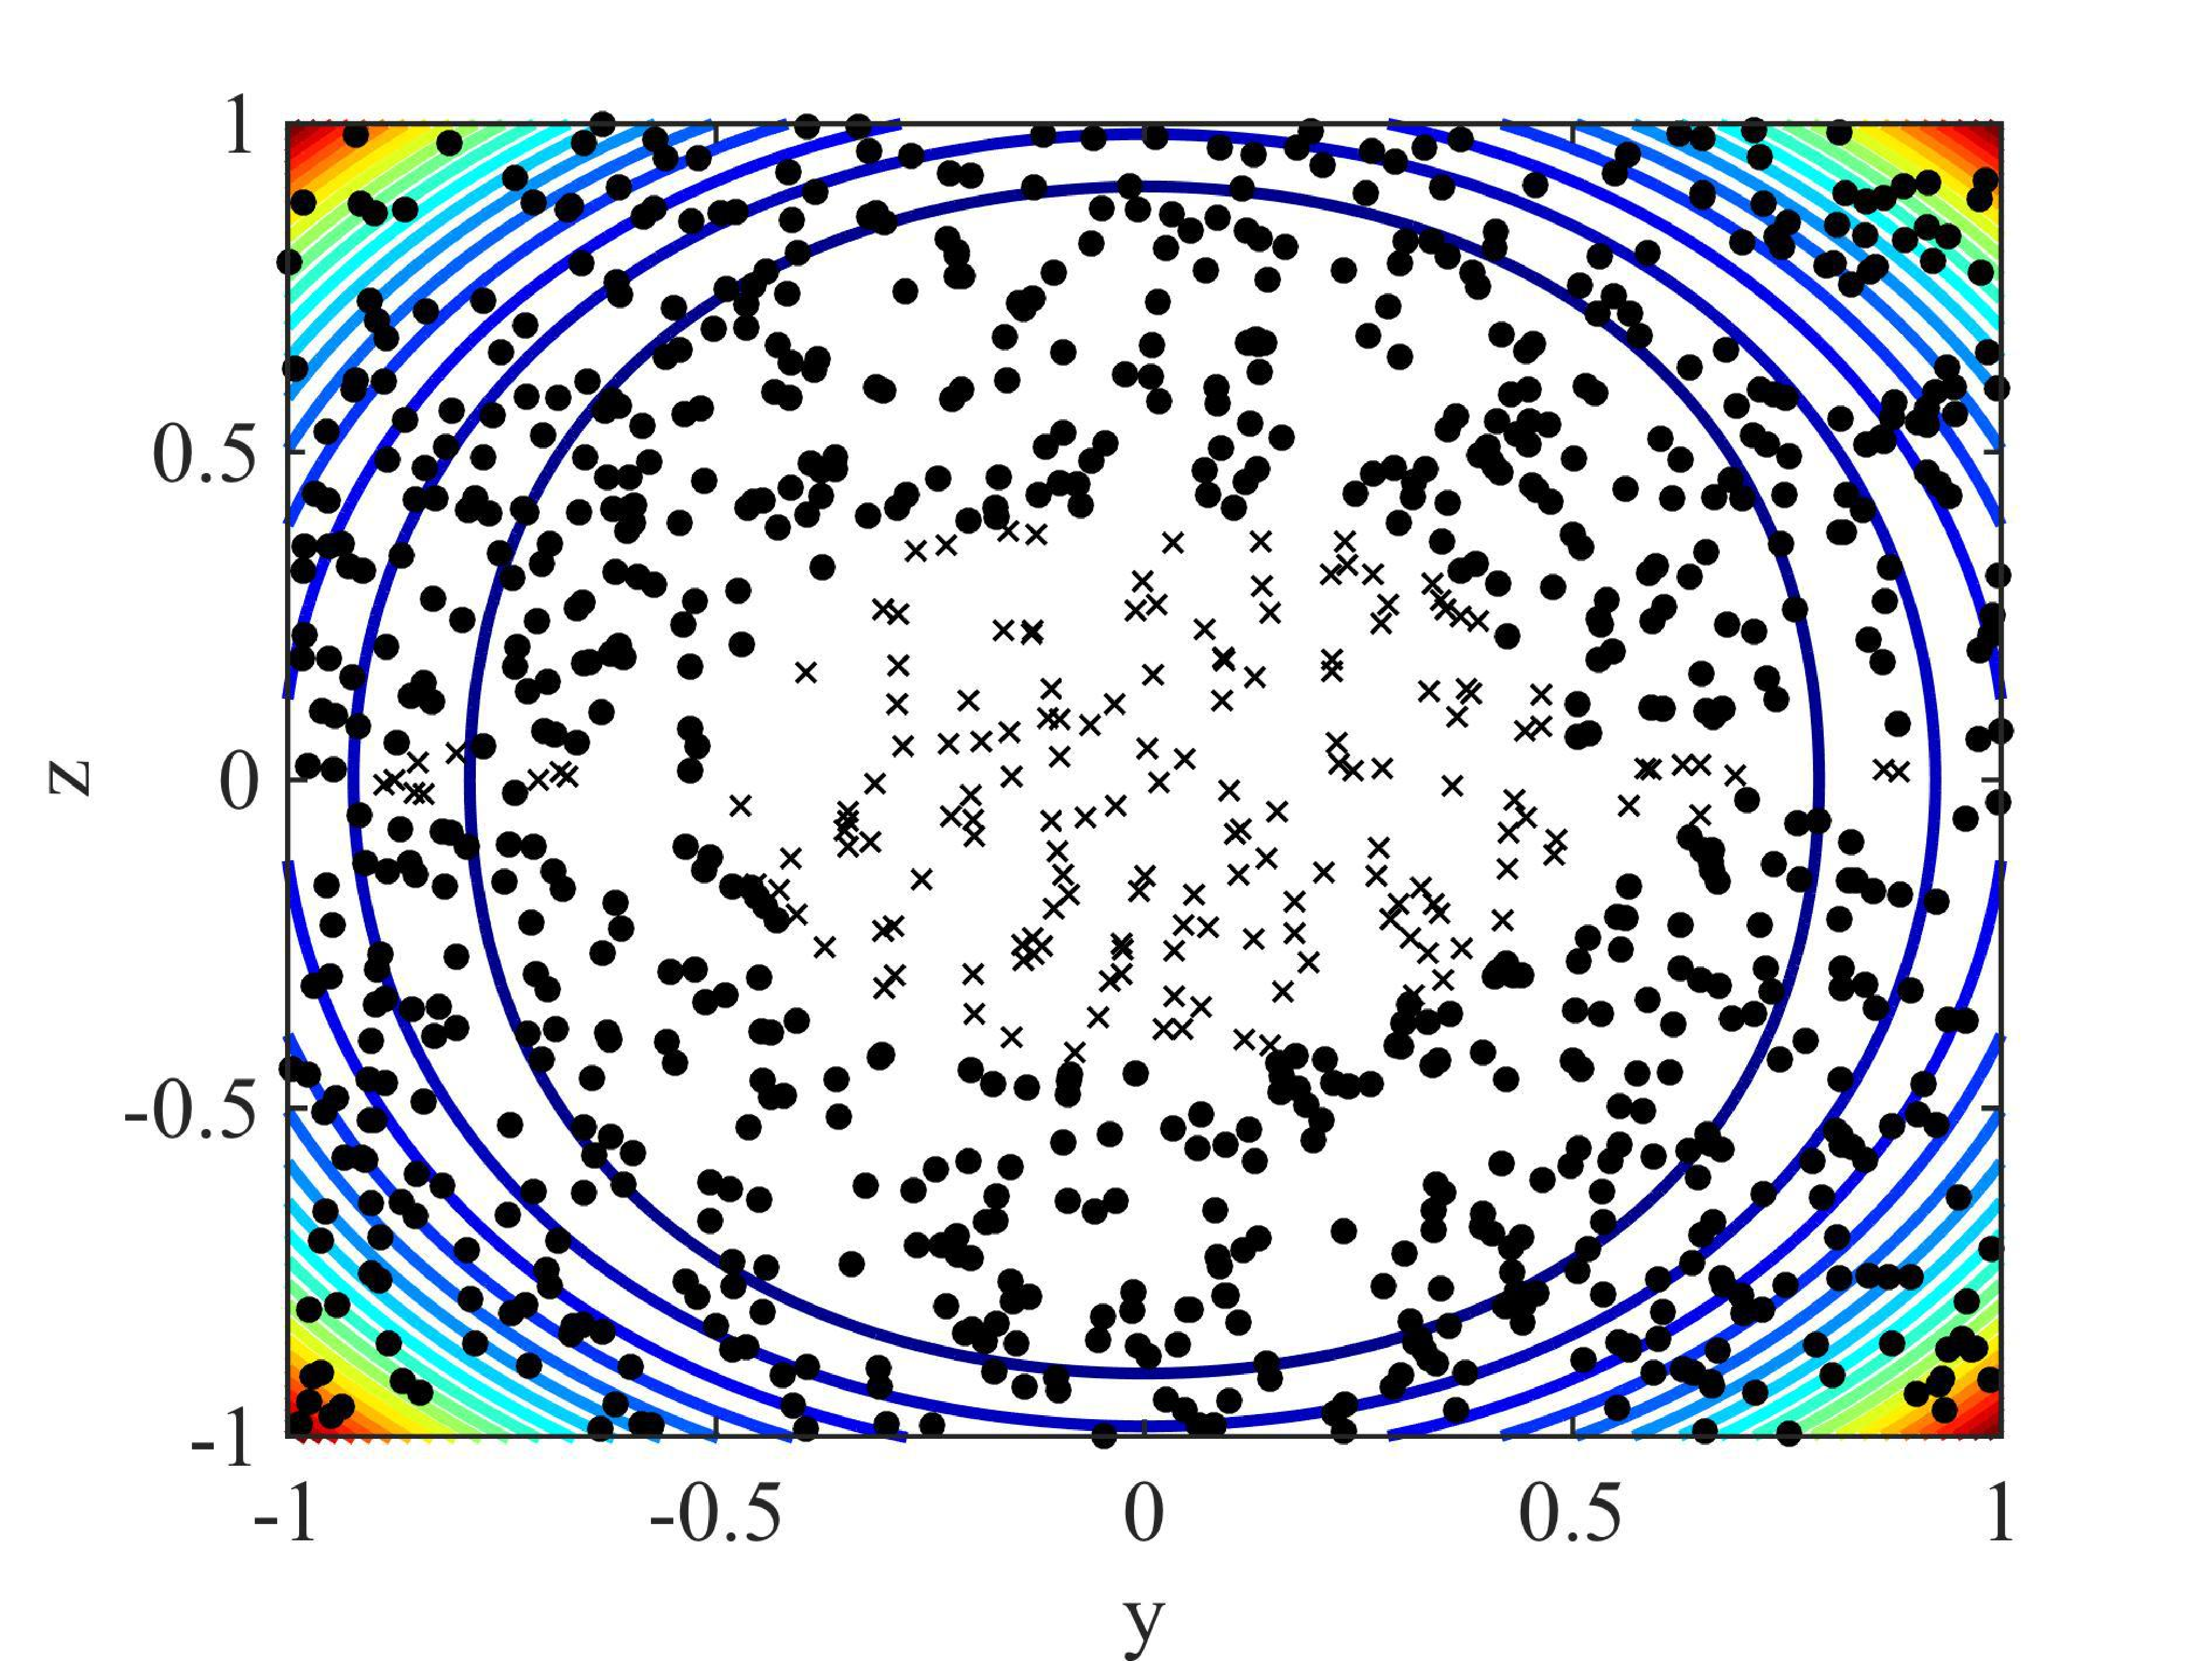
\includegraphics[width=0.47\textwidth]
   {figs/aniso_uniaxial_cartesian_random.pdf}
 } \subfigure[Stereographic]{
   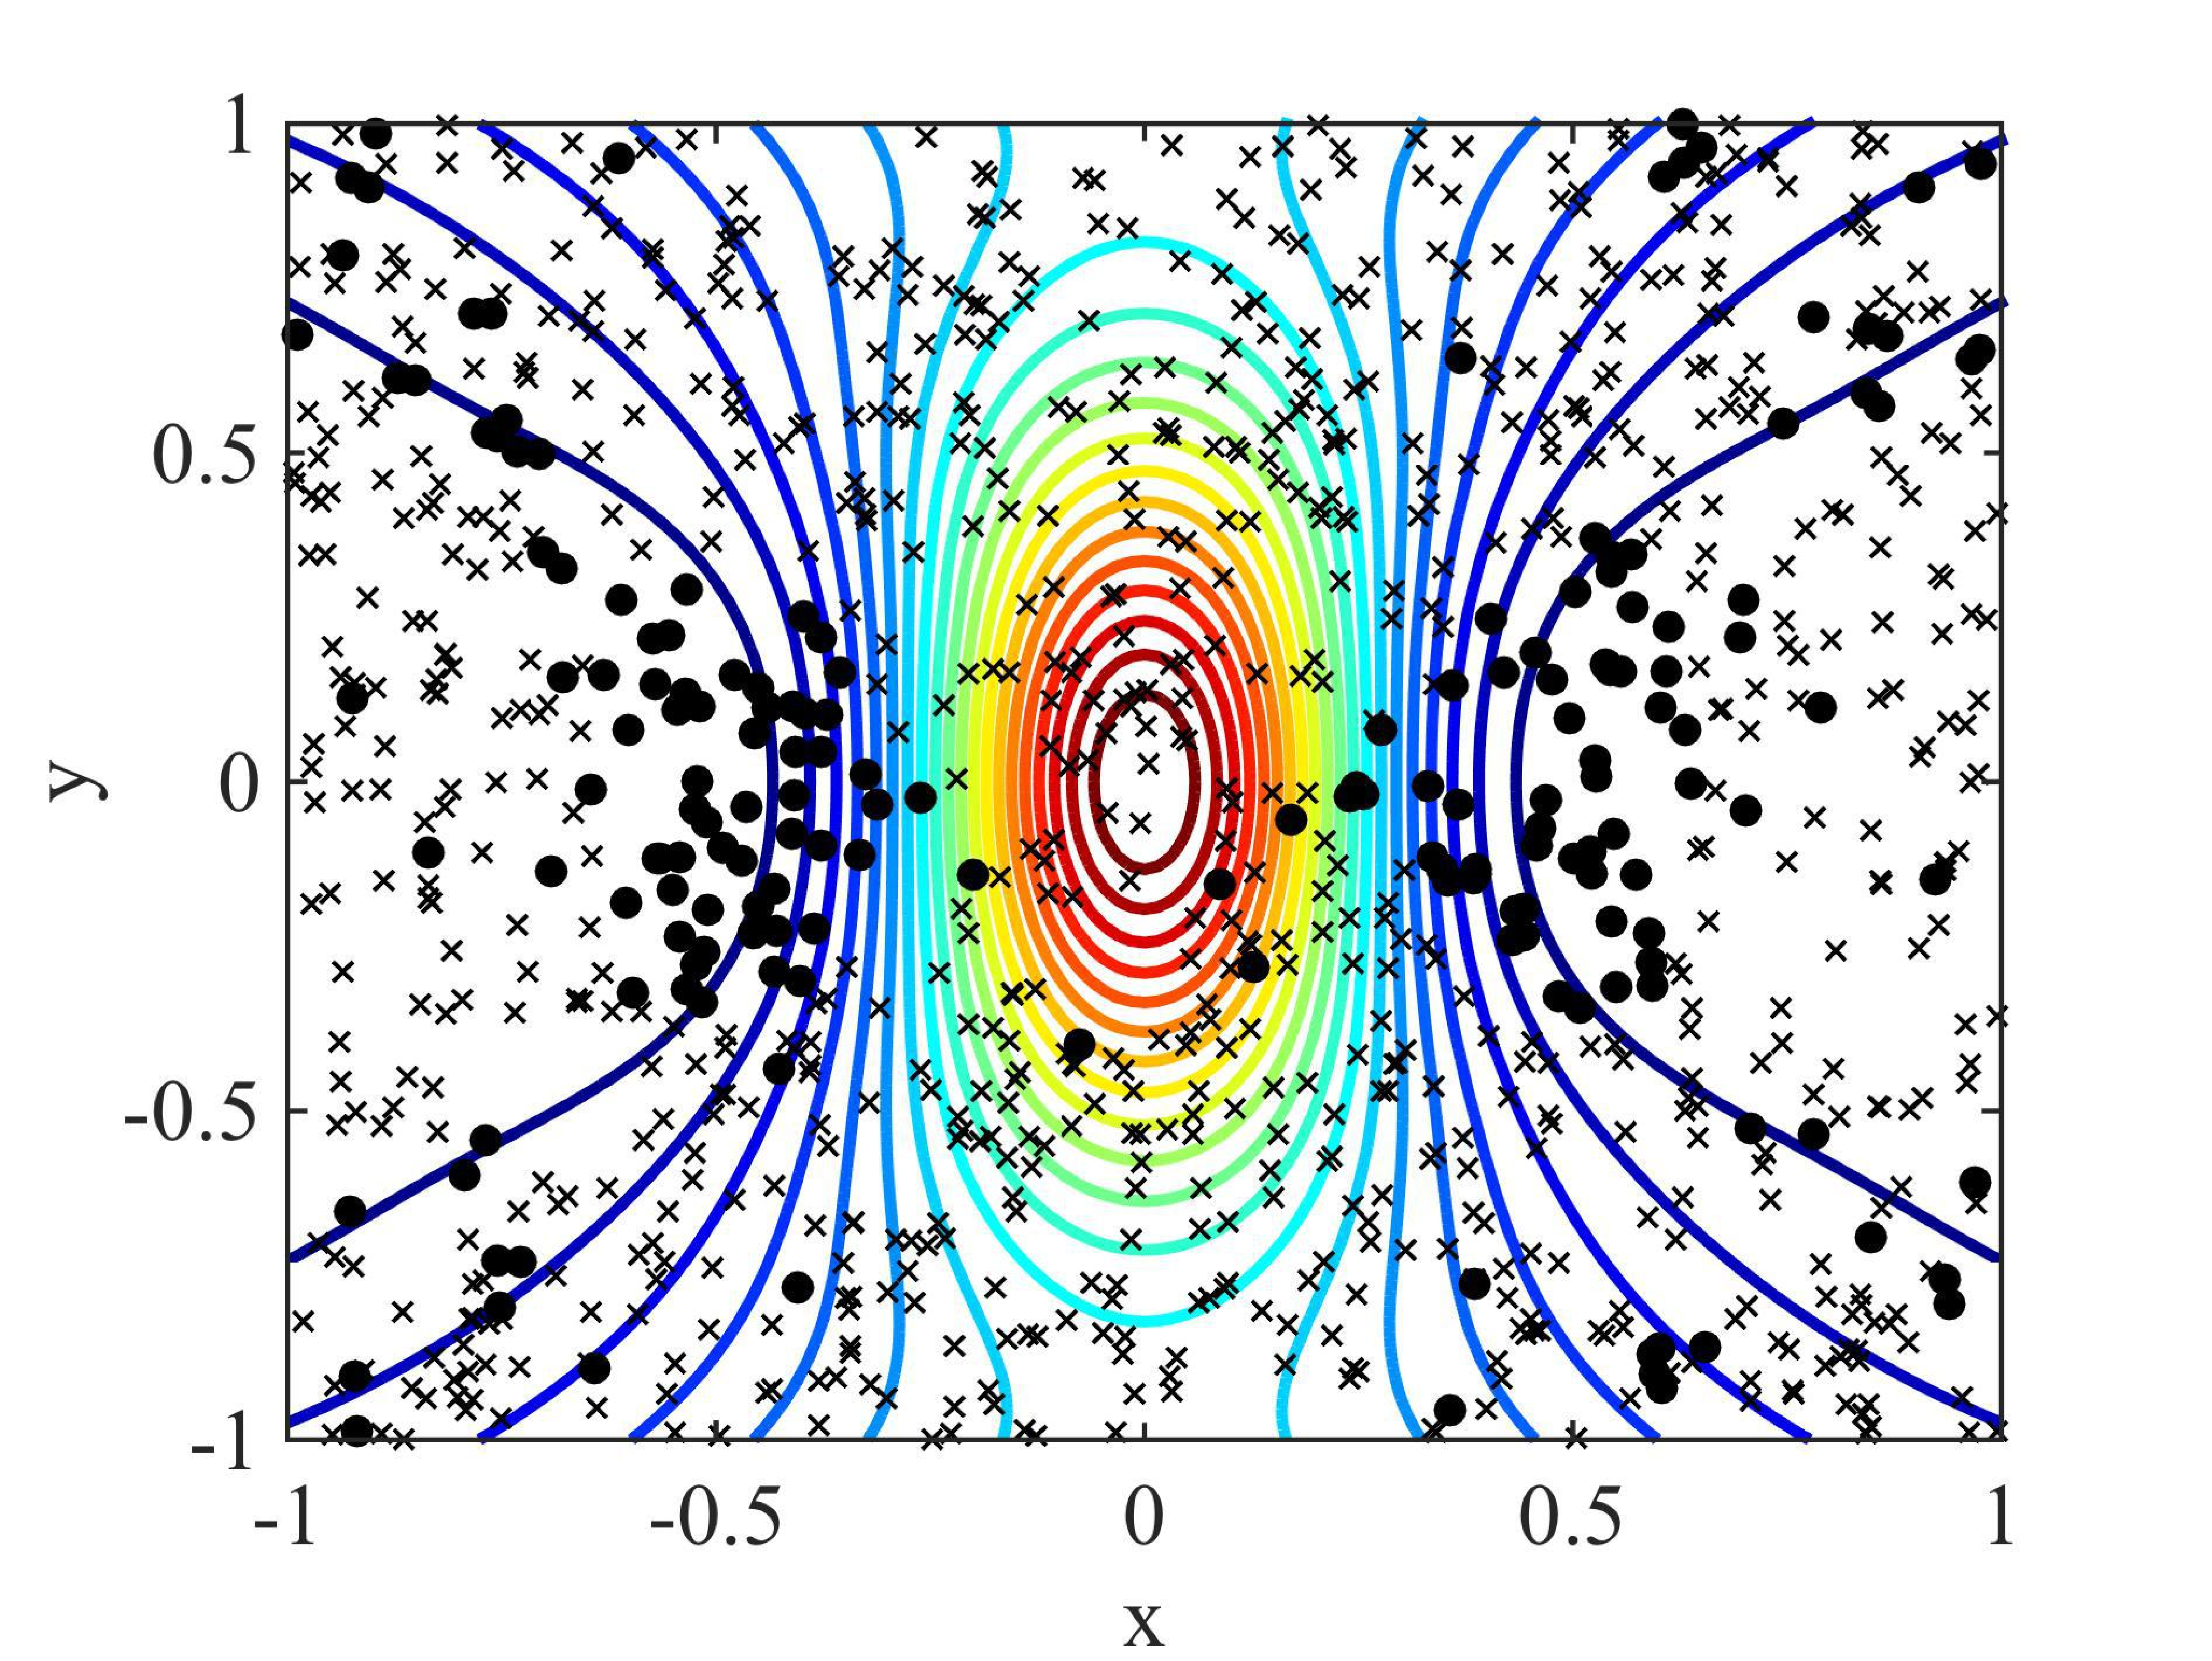
\includegraphics[width=0.47\textwidth]
   {figs/aniso_uniaxial_stereographic_random.pdf}
 } \subfigure[Tangent]{
   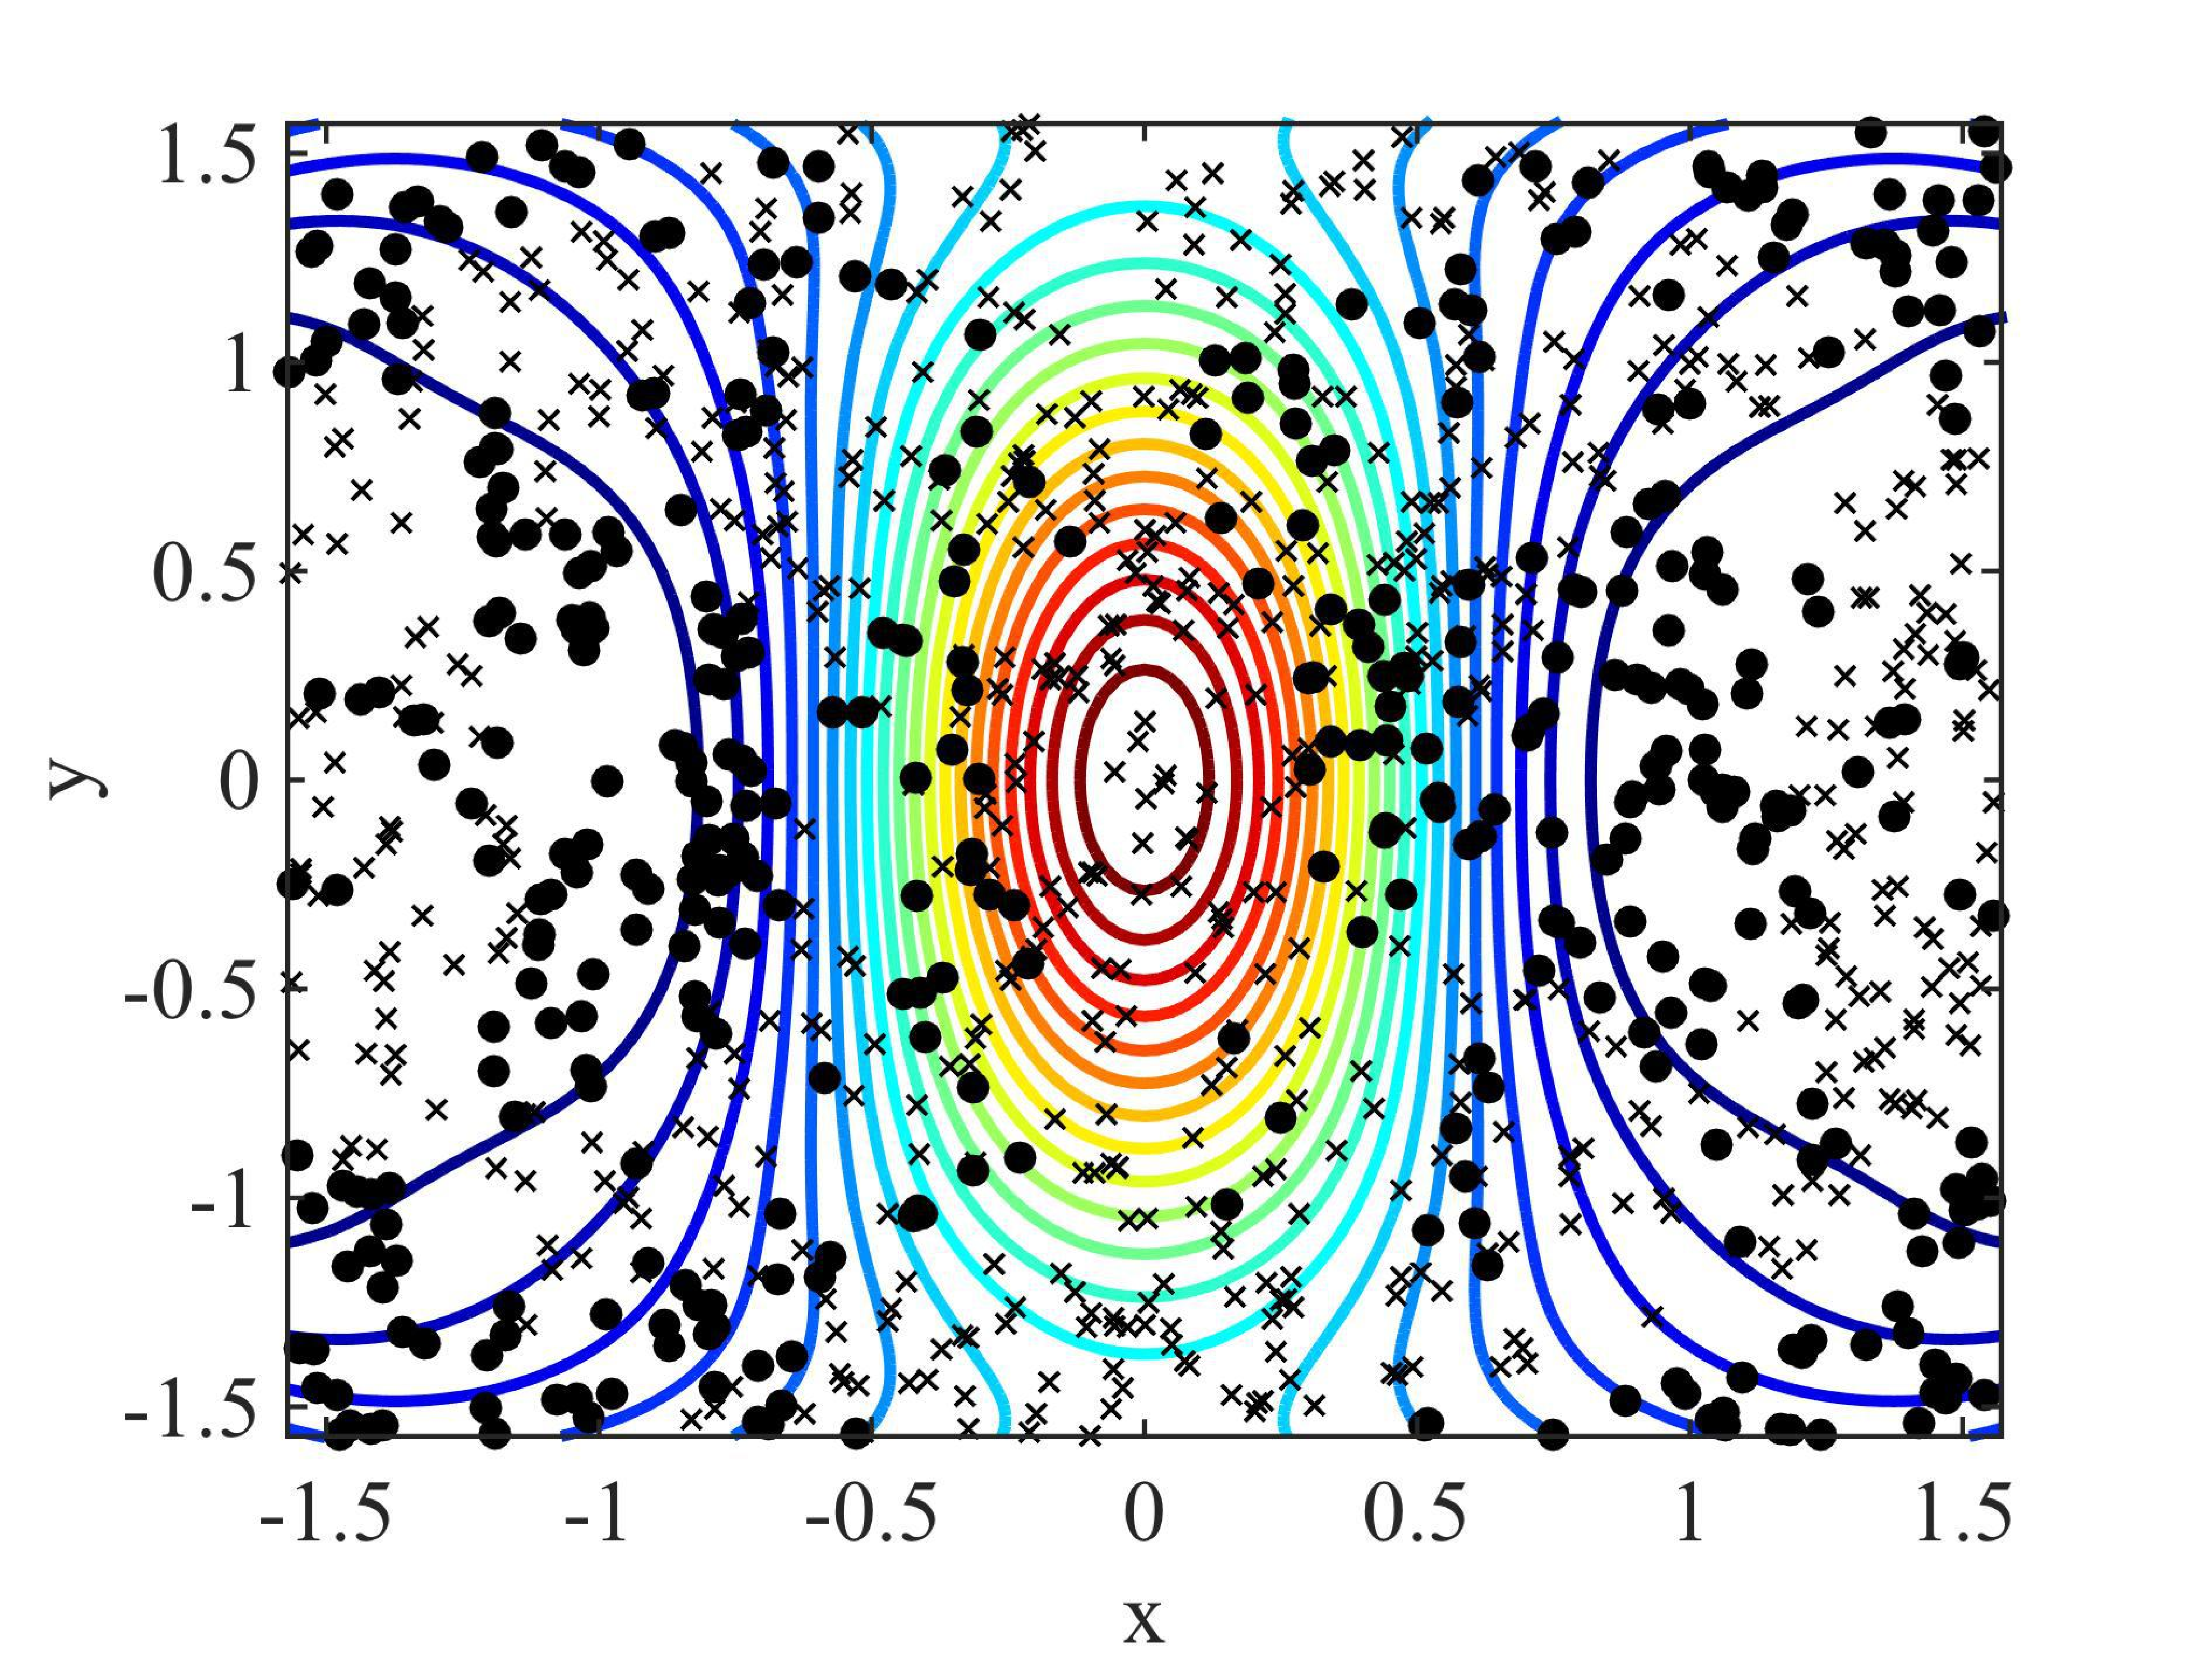
\includegraphics[width=0.47\textwidth]
   {figs/aniso_uniaxial_tangent_random.pdf}
 }
   \caption{Anisotropic finite deformation model: results of the
     Newton iterative scheme with a single random initial guess
     plotted on contours of the determinant function at
     bifurcation. A solid circle ($\bullet$) indicates that the
     initial point leads to a successful detection of bifurcation and
     its directions. A cross ($\times$) indicates failure. A total of
     1000 random trials are performed for each parametrization.}
   \label{fig:aniso-uniaxial-robust}
 \end{figure}

As in the case of the small deformation model example in Section
\ref{subsec:isotropic}, the Cartesian parametrization performs better
in terms of trade-off between computational efficiency and
robustness. In a non-linear large-scale finite element simulation,
this optimal trade-off between computational efficiency and robustness
becomes critical. The Cartesian parametrization thus provides a
valuable tool in numerical bifurcation analysis.

\section{Conclusion}

In this work we examine the numerical performance of five different
parametrizations for the detection of the loss of the ellipticity
condition for the analysis of material instabilities. An algorithm
based on an initial sampling on a parametric grid followed by an
iterative Newton scheme is introduced as a robust and efficient method
for the detection of the bifurcation condition. In addition, we
introduce a new parametrization that we term Cartesian for the
representation of the normal vector that defines the acoustic tensor
in terms of the tangent moduli tensor. We demonstrate with numerical
examples that the Cartesian parametrization offers the best
performance in terms of computational efficiency and robustenss as
compared with other four parametrizations. In summary, we find that:

\begin{enumerate}
\item
The parametrization of the normal vector significantly affects the
complexity of the objective function to be minimized, which in turn
influences the computational efficiency and robustness of the
algorithm used for the detection of bifurcation.

\item
The commonly used spherical parametrization is efficient provided
that the initial sampling interval is fine enough and the initial
guess is a good approximation to the minimum.

\item
The stereographic and tangent parametrizations are the least
robust, \ie, they are more likely to have convergence issues. The
projective parametrization is much more expensive.

\item
The Cartesian parametrization is the most robust for the material
models and loading conditions tested. It is also computationally
efficient. The Cartesian parametrization represents an optimal
trade-off between computational efficiency and robustness and provides
a valuable tool for efficient and robust numerical analysis of
material instability in large-scale finite element analysis.
\end{enumerate}

\bibliographystyle{unsrtnat}
\bibliography{acpami}

\end{document}
